\chapter{Basic Usage}





In interactive code examples that follow, it will be assumed that all items in the mpFormulaPy
namespace have been imported:

\lstset{language={Python}}
\begin{lstlisting}
>>> from mpFormulaPy import *
\end{lstlisting}

Importing everything can be convenient, especially when using mpFormulaPy interactively, but be careful when mixing mpFormulaPy with other libraries! To avoid inadvertently overriding other functions or objects, explicitly import only the needed objects, or use the mpFormulaPy. or mp.namespaces:


\lstset{language={Python}}
\begin{lstlisting}
from mpFormulaPy import sin, cos
sin(1), cos(1)
import mpFormulaPy
mpFormulaPy.sin(1), mpFormulaPy.cos(1)
from mpFormulaPy import mp # mp context object -- to be explained
mp.sin(1), mp.cos(1)>>> from mpFormulaPy import *
\end{lstlisting}



\section{Number types}
Mpmath provides the following numerical types:

\begin{verbatim}
Class Description
mpf Real float
mpc Complex float
matrix Matrix
\end{verbatim}


Currently missing: decimals. The MPD reference is \cite{mpd_2012}


The following section will provide a very short introduction to the types mpf and mpc. Intervals and matrices are described further in the documentation chapters on interval arithmetic and matrices / linear algebra.

\vpara
The mpf type is analogous to Python's built-in float. It holds a real number or one of the special values inf (positive infinity), -inf (negative infinity) and nan (not-a-number, indicating an indeterminate result). You can create mpf instances from strings, integers, floats, and
other mpf instances:

\lstset{language={Python}}
\begin{lstlisting}
>>> mpf(4)
mpf('4.0')
>>> mpf(2.5)
mpf('2.5')
>>> mpf("1.25e6")
mpf('1250000.0')
>>> mpf(mpf(2))
mpf('2.0')
>>> mpf("inf")
mpf('+inf')
\end{lstlisting}


The mpc type represents a complex number in rectangular form as a pair of mpf instances. It can be constructed from a Python complex, a real number, or a pair of real numbers:

\lstset{language={Python}}
\begin{lstlisting}
>>> mpc(2,3)
mpc(real='2.0', imag='3.0')
>>> mpc(complex(2,3)).imag
mpf('3.0')
\end{lstlisting}


You can mix mpf and mpc instances with each other and with Python numbers:

\lstset{language={Python}}
\begin{lstlisting}
>>> mpf(3) + 2*mpf('2.5') + 1.0
mpf('9.0')
>>> mp.dps = 15 # Set precision (see below)
>>> mpc(1j)**0.5
mpc(real='0.70710678118654757', imag='0.70710678118654757')
\end{lstlisting}


\subsection{Setting the precision} 

Mpmath uses a global working precision; it does not keep track of the precision or accuracy of individual numbers. Performing an arithmetic operation or calling mpf() rounds the result to the current working precision. The working precision is controlled by a context object called mp, which has the following default states:

\lstset{language={Python}}
\begin{lstlisting}
>>> from mpFormulaPy import *
>>> mp.dps
25
>>> mp.prec
86
>>> mp.trap_complex
False
>>>
\end{lstlisting}


The term prec denotes the binary precision (measured in bits) while dps (short for decimal places) is the decimal precision. Binary and decimal precision are related roughly according to the formula prec = 3.33*dps. For example, it takes a precision of roughly 333 bits to hold an approximation of pi that is accurate to 100 decimal places (actually slightly more than 333 bits is used).

\vpara
Changing either precision property of the mp object automatically updates the other; usually you just want to change the dps value:

\lstset{language={Python}}
\begin{lstlisting}
>>> mp.dps = 100
>>> mp.dps
100
>>> mp.prec
336
\end{lstlisting}


When the precision has been set, all mpf operations are carried out at that precision:

\lstset{language={Python}}
\begin{lstlisting}
>>> mp.dps = 50
>>> mpf(1) / 6
mpf('0.16666666666666666666666666666666666666666666666666656')
>>> mp.dps = 25
>>> mpf(2) ** mpf('0.5')
mpf('1.414213562373095048801688713')
\end{lstlisting}

The precision of complex arithmetic is also controlled by the mp object:

\lstset{language={Python}}
\begin{lstlisting}
>>> mp.dps = 10
>>> mpc(1,2) / 3
mpc(real='0.3333333333321', imag='0.6666666666642')
\end{lstlisting}


There is no restriction on the magnitude of numbers. An mpf can for example hold an approximation of a large Mersenne prime:

\lstset{language={Python}}
\begin{lstlisting}
>>> mp.dps = 15
>>> print mpf(2)**32582657 - 1
1.24575026015369e+9808357
\end{lstlisting}


Or why not 1 googolplex:

\lstset{language={Python}}
\begin{lstlisting}
>>> print mpf(10) ** (10**100)
1.0e+100000000000000000000000000000000000000000000000000...
\end{lstlisting}


The (binary) exponent is stored exactly and is independent of the precision.


\subsection{Temporarily changing the precision}  

It is often useful to change the precision during only part of a calculation. A way to temporarily increase the precision and then restore it is as follows:

\lstset{language={Python}}
\begin{lstlisting}
>>> mp.prec += 2
>>> # do_something()
>>> mp.prec -= 2
\end{lstlisting}


As of Python 2.5, the with statement along with the mpFormulaPy functions workprec, workdps, extraprec and extradps can be used to temporarily change precision in a more safe manner:

\lstset{language={Python}}
\begin{lstlisting}
>>> from __future__ import with_statement
>>> with workdps(20):
... print mpf(1)/7
... with extradps(10):
... print mpf(1)/7
...
0.14285714285714285714
0.142857142857142857142857142857
>>> mp.dps
15
\end{lstlisting}


The with statement ensures that the precision gets reset when exiting the block, even in the case that an exception is raised. (The effect of the with statement can be emulated in Python 2.4 by using a try/finally block.)

The workprec family of functions can also be used as function decorators:

\lstset{language={Python}}
\begin{lstlisting}
>>> @workdps(6)
... def f():
... return mpf(1)/3
...
>>> f()
mpf('0.33333331346511841')
\end{lstlisting}


Some functions accept the prec and dps keyword arguments and this will override the global working precision. Note that this will not affect the precision at which the result is printed, so to get all digits, you must either use increase precision afterward when printing or use nstr/nprint:

\lstset{language={Python}}
\begin{lstlisting}
>>> mp.dps = 15
>>> print exp(1)
2.71828182845905
>>> print exp(1, dps=50) # Extra digits won't be printed
2.71828182845905
>>> nprint(exp(1, dps=50), 50)
2.7182818284590452353602874713526624977572470937
\end{lstlisting}


Finally, instead of using the global context object mp, you can create custom contexts and work with methods of those instances instead of global functions. The working precision will be local to each context object:

\lstset{language={Python}}
\begin{lstlisting}
>>> mp2 = mp.clone()
>>> mp.dps = 10
>>> mp2.dps = 20
>>> print mp.mpf(1) / 3
0.3333333333
>>> print mp2.mpf(1) / 3
0.33333333333333333333
\end{lstlisting}


Note: the ability to create multiple contexts is a new feature that is only partially implemented. Not all mpFormulaPy functions are yet available as context-local methods. In the present version, you are likely to encounter bugs if you try mixing different contexts.


\subsection{Providing correct input}  

Note that when creating a new mpf, the value will at most be as accurate as the input. Be careful when mixing mpFormulaPy numbers with Python floats. When working at high precision, fractional mpf values should be created from strings or integers:

\lstset{language={Python}}
\begin{lstlisting}
>>> mp.dps = 30
>>> mpf(10.9) # bad
mpf('10.9000000000000003552713678800501')
>>> mpf('10.9') # good
mpf('10.8999999999999999999999999999997')
>>> mpf(109) / mpf(10) # also good
mpf('10.8999999999999999999999999999997')
>>> mp.dps = 15
\end{lstlisting}


(Binary fractions such as 0.5, 1.5, 0.75, 0.125, etc, are generally safe as input, however, since those can be represented exactly by Python floats.)


\subsection{Printing}  

By default, the repr() of a number includes its type signature. This way eval can be used to recreate a number from its string representation:

\lstset{language={Python}}
\begin{lstlisting}
>>> eval(repr(mpf(2.5)))
mpf('2.5')
\end{lstlisting}


Prettier output can be obtained by using str() or print, which hide the mpf and mpc signatures and also suppress rounding artifacts in the last few digits:

\lstset{language={Python}}
\begin{lstlisting}
>>> mpf("3.14159")
mpf('3.1415899999999999')
>>> print mpf("3.14159")
3.14159
>>> print mpc(1j)**0.5
(0.707106781186548 + 0.707106781186548j)
\end{lstlisting}


Setting the mp.pretty option will use the str()-style output for repr() as well:

\lstset{language={Python}}
\begin{lstlisting}
>>> mp.pretty = True
>>> mpf(0.6)
0.6
>>> mp.pretty = False
>>> mpf(0.6)
mpf('0.59999999999999998')
\end{lstlisting}


The number of digits with which numbers are printed by default is determined by the working precision. To specify the number of digits to show without changing the working precision, use mpFormulaPy.nstr() and mpFormulaPy.nprint():

\lstset{language={Python}}
\begin{lstlisting}
>>> a = mpf(1) / 6
>>> a
mpf('0.16666666666666666')
>>> nstr(a, 8)
'0.16666667'
>>> nprint(a, 8)
0.16666667
>>> nstr(a, 50)
'0.16666666666666665741480812812369549646973609924316'
\end{lstlisting}














\subsection{Contexts}  

High-level code in mpFormulaPy is implemented as methods on a 'context object'. The context implements arithmetic, type conversions and other fundamental operations. The context also holds settings such as precision, and stores cache data. A few different contexts (with a
mostly compatible interface) are provided so that the high-level algorithms can be used with different implementations of the underlying arithmetic, allowing different features and speed/accuracy tradeoffs. Currently, mpFormulaPy provides the following contexts:

\vpara
Arbitrary-precision arithmetic (mp)

A faster Cython-based version of mp (used by default in Sage, and currently only available there)

Arbitrary-precision interval arithmetic (iv)

Double-precision arithmetic using Python's builtin float and complex types (fp)

\vpara
Most global functions in the global mpFormulaPy namespace are actually methods of the mp context. This fact is usually transparent to the user, but sometimes shows up in the form of an initial parameter called 'ctx' visible in the help for the function:

\lstset{language={Python}}
\begin{lstlisting}
>>> import mpFormulaPy
>>> help(mpFormulaPy.fsum)
Help on method fsum in module mpFormulaPy.ctx_mp_python:
fsum(ctx, terms, absolute=False, squared=False) method of mpFormulaPy.ctx_mp.MPContext ins
Calculates a sum containing a finite number of terms (for infinite
series, see :func:`~mpFormulaPy.nsum`). The terms will be converted to
...
\end{lstlisting}



The following operations are equivalent:

\lstset{language={Python}}
\begin{lstlisting}
>>> mpFormulaPy.mp.dps = 15; mpFormulaPy.mp.pretty = False
>>> mpFormulaPy.fsum([1,2,3])
mpf('6.0')
>>> mpFormulaPy.mp.fsum([1,2,3])
mpf('6.0')
\end{lstlisting}


The corresponding operation using the fp context:

\lstset{language={Python}}
\begin{lstlisting}
>>> mpFormulaPy.fp.fsum([1,2,3])
6.0
\end{lstlisting}


\subsection{Common interface}  

ctx.mpf creates a real number:

\lstset{language={Python}}
\begin{lstlisting}
>>> from mpFormulaPy import mp, fp
>>> mp.mpf(3)
mpf('3.0')
>>> fp.mpf(3)
3.0
\end{lstlisting}


ctx.mpc creates a complex number:

\lstset{language={Python}}
\begin{lstlisting}
>>> mp.mpc(2,3)
mpc(real='2.0', imag='3.0')
>>> fp.mpc(2,3)
(2+3j)
\end{lstlisting}


ctx.matrix creates a matrix:

\lstset{language={Python}}
\begin{lstlisting}
>>> mp.matrix([[1,0],[0,1]])
matrix(
[['1.0', '0.0'],
['0.0', '1.0']])
>>> _[0,0]
mpf('1.0')
>>> fp.matrix([[1,0],[0,1]])
matrix(
[['1.0', '0.0'],
['0.0', '1.0']])
>>> _[0,0]
1.0
\end{lstlisting}


ctx.prec holds the current precision (in bits):

\lstset{language={Python}}
\begin{lstlisting}
>>> mp.prec
53
>>> fp.prec
53
\end{lstlisting}


ctx.dps holds the current precision (in digits):

\lstset{language={Python}}
\begin{lstlisting}
>>> mp.dps
15
>>> fp.dps
15
\end{lstlisting}


ctx.pretty controls whether objects should be pretty-printed automatically by repr(). Prettyprinting for mp numbers is disabled by default so that they can clearly be distinguished from Python numbers and so that eval(repr(x)) == x works:

\lstset{language={Python}}
\begin{lstlisting}
>>> mp.mpf(3)
mpf('3.0')
>>> mpf = mp.mpf
>>> eval(repr(mp.mpf(3)))
mpf('3.0')
>>> mp.pretty = True
>>> mp.mpf(3)
3.0
>>> fp.matrix([[1,0],[0,1]])
matrix(
[['1.0', '0.0'],
['0.0', '1.0']])
>>> fp.pretty = True
>>> fp.matrix([[1,0],[0,1]])
[1.0 0.0]
[0.0 1.0]
>>> fp.pretty = False
>>> mp.pretty = False
\end{lstlisting}



\subsection{Arbitrary-precision floating-point (mp)}  

The mp context is what most users probably want to use most of the time, as it supports the most functions, is most well-tested, and is implemented with a high level of optimization. Nearly all examples in this documentation use mp functions.

See Basic usage for a description of basic usage.


\subsection{Arbitrary-precision interval arithmetic (iv)}  

The iv.mpf type represents a closed interval $[a,]$; that is, the set $\{x: a \leq x \leq b\}$, where $a$ and $b $ are arbitrary-precision floating-point values, possibly $\pm\infty$. The iv.mpc type represents a rectangular complex interval $[a,b] + [c,d]i$; that is, the set $\{z=x+iy: a \leq x \leq b \wedge c \leq y \leq d\}$.

\vpara
Interval arithmetic provides rigorous error tracking. If  $f$ is a mathematical function and $\hat{f}$ is its interval arithmetic version, then the basic guarantee of interval arithmetic is that $f(v) \subseteq \hat{f}(v)$ for any input interval $v$. Put differently, if an interval represents the known uncertainty for a fixed number, any sequence of interval operations will produce an interval that contains what would be the result of applying the same sequence of operations to the exact number. The principal drawbacks of interval arithmetic are speed (iv arithmetic is typically at least two times slower than mp arithmetic) and that it sometimes provides far too pessimistic bounds.

\vpara
Note: The support for interval arithmetic in mpFormulaPy is still experimental, and many functions do not yet properly support intervals. Please use this feature with caution.

\vpara
Intervals can be created from single numbers (treated as zero-width intervals) or pairs of endpoint numbers. Strings are treated as exact decimal numbers. Note that a Python float like 0.1 generally does not represent the same number as its literal; use '0.1' instead:

\lstset{language={Python}}
\begin{lstlisting}
>>> from mpFormulaPy import iv
>>> iv.dps = 15; iv.pretty = False
>>> iv.mpf(3)
mpi('3.0', '3.0')
>>> print iv.mpf(3)
[3.0, 3.0]
>>> iv.pretty = True
>>> iv.mpf([2,3])
[2.0, 3.0]
>>> iv.mpf(0.1) # probably not intended
[0.10000000000000000555, 0.10000000000000000555]
>>> iv.mpf('0.1') # good, gives a containing interval
[0.099999999999999991673, 0.10000000000000000555]
>>> iv.mpf(['0.1', '0.2'])
[0.099999999999999991673, 0.2000000000000000111]
\end{lstlisting}


The fact that '0.1' results in an interval of nonzero width indicates that 1/10 cannot be represented using binary floating-point numbers at this precision level (in fact, it cannot be represented exactly at any precision).

\vpara
Intervals may be infinite or half-infinite:

\lstset{language={Python}}
\begin{lstlisting}
>>> print 1 / iv.mpf([2, 'inf'])
[0.0, 0.5]
\end{lstlisting}


The equality testing operators $==$ and $!=$ check whether their operands are identical as intervals; that is, have the same endpoints. The ordering operators $<$,  $<=$,  $>$ and $>=$ permit inequality testing using triple-valued logic: a guaranteed inequality returns True or False while an indeterminate inequality returns None:

\lstset{language={Python}}
\begin{lstlisting}
>>> iv.mpf([1,2]) == iv.mpf([1,2])
True
>>> iv.mpf([1,2]) != iv.mpf([1,2])
False
>>> iv.mpf([1,2]) <= 2
True
>>> iv.mpf([1,2]) > 0
True
>>> iv.mpf([1,2]) < 1
False
>>> iv.mpf([1,2]) < 2 # returns None
>>> iv.mpf([2,2]) < 2
False
>>> iv.mpf([1,2]) <= iv.mpf([2,3])
True
>>> iv.mpf([1,2]) < iv.mpf([2,3]) # returns None
>>> iv.mpf([1,2]) < iv.mpf([-1,0])
False
\end{lstlisting}


The in operator tests whether a number or interval is contained in another interval:

\lstset{language={Python}}
\begin{lstlisting}
>>> iv.mpf([0,2]) in iv.mpf([0,10])
True
>>> 3 in iv.mpf(['-inf', 0])
False
\end{lstlisting}


Intervals have the properties .a, .b (endpoints), .mid, and .delta (width):

\lstset{language={Python}}
\begin{lstlisting}
>>> x = iv.mpf([2, 5])
>>> x.a
[2.0, 2.0]
>>> x.b
[5.0, 5.0]
>>> x.mid
[3.5, 3.5]
>>> x.delta
[3.0, 3.0]
\end{lstlisting}


Some transcendental functions are supported:

\lstset{language={Python}}
\begin{lstlisting}
>>> iv.dps = 15
>>> mp.dps = 15
>>> iv.mpf([0.5,1.5]) ** iv.mpf([0.5, 1.5])
[0.35355339059327373086, 1.837117307087383633]
>>> iv.exp(0)
[1.0, 1.0]
>>> iv.exp(['-inf','inf'])
[0.0, +inf]
>>>
>>> iv.exp(['-inf',0])
[0.0, 1.0]
>>> iv.exp([0,'inf'])
[1.0, +inf]
>>> iv.exp([0,1])
[1.0, 2.7182818284590455349]
>>>
>>> iv.log(1)
[0.0, 0.0]
>>> iv.log([0,1])
[-inf, 0.0]
>>> iv.log([0,'inf'])
[-inf, +inf]
>>> iv.log(2)
[0.69314718055994528623, 0.69314718055994539725]
>>>
>>> iv.sin([100,'inf'])
[-1.0, 1.0]
>>> iv.cos(['-0.1','0.1'])
[0.99500416527802570954, 1.0]
\end{lstlisting}


Interval arithmetic is useful for proving inequalities involving irrational numbers. Naive use of mp arithmetic may result in wrong conclusions, such as the following:

\lstset{language={Python}}
\begin{lstlisting}
>>> mp.dps = 25
>>> x = mp.exp(mp.pi*mp.sqrt(163))
>>> y = mp.mpf(640320**3+744)
>>> print x
262537412640768744.0000001
>>> print y
262537412640768744.0
>>> x > y
True
\end{lstlisting}


But the correct result is $e^{\pi\sqrt{163}} < 262537412640768744$, as can be seen by increasing the precision:

\lstset{language={Python}}
\begin{lstlisting}
>>> mp.dps = 50
>>> print mp.exp(mp.pi*mp.sqrt(163))
262537412640768743.99999999999925007259719818568888
\end{lstlisting}


With interval arithmetic, the comparison returns None until the precision is large enough for $x-y$ to have a definite sign:

\lstset{language={Python}}
\begin{lstlisting}
>>> iv.dps = 15
>>> iv.exp(iv.pi*iv.sqrt(163)) > (640320**3+744)
>>> iv.dps = 30
>>> iv.exp(iv.pi*iv.sqrt(163)) > (640320**3+744)
>>> iv.dps = 60
>>> iv.exp(iv.pi*iv.sqrt(163)) > (640320**3+744)
False
>>> iv.dps = 15
\end{lstlisting}


\subsection{Fast low-precision arithmetic (fp)}  

Although mpFormulaPy is generally designed for arbitrary-precision arithmetic, many of the high-level algorithms work perfectly well with ordinary Python float and complex numbers, which use hardware double precision (on most systems, this corresponds to 53 bits of precision). 

Whereas the global functions (which are methods of the mp object) always
convert inputs to mpFormulaPy numbers, the fp object instead converts them to float or complex, and in some cases employs basic functions optimized for double precision. When large amounts of function evaluations (numerical integration, plotting, etc) are required, and when
fp arithmetic provides sufficient accuracy, this can give a significant speedup over mp arithmetic.

\vpara
To take advantage of this feature, simply use the fp prefix, i.e. write fp.func instead of func or mp.func:

\lstset{language={Python}}
\begin{lstlisting}
>>> u = fp.erfc(2.5)
>>> print u
0.000406952017445
>>> type(u)
<type 'float'>
>>> mp.dps = 15
>>> print mp.erfc(2.5)
0.000406952017444959
>>> fp.matrix([[1,2],[3,4]]) ** 2
matrix(
[['7.0', '10.0'],
['15.0', '22.0']])
>>>
>>> type(_[0,0])
<type 'float'>
>>> print fp.quad(fp.sin, [0, fp.pi]) # numerical integration
2.0
\end{lstlisting}


The fp context wraps Python's math and cmath modules for elementary functions. It supports both real and complex numbers and automatically generates complex results for real inputs (math raises an exception):

\lstset{language={Python}}
\begin{lstlisting}
>>> fp.sqrt(5)
2.23606797749979
>>> fp.sqrt(-5)
2.23606797749979j
>>> fp.sin(10)
-0.5440211108893698
>>> fp.power(-1, 0.25)
(0.7071067811865476+0.7071067811865475j)
>>> (-1) ** 0.25
Traceback (most recent call last):
...
ValueError: negative number cannot be raised to a fractional power
\end{lstlisting}


The prec and dps attributes can be changed (for interface compatibility with the mp context) but this has no effect:

\lstset{language={Python}}
\begin{lstlisting}
>>> fp.prec
53
>>> fp.dps
15
>>> fp.prec = 80
>>> fp.prec
53
>>> fp.dps
15
\end{lstlisting}


Due to intermediate rounding and cancellation errors, results computed with fp arithmetic may be much less accurate than those computed with mp using an equivalent precision (mp.prec = 53), since the latter often uses increased internal precision. The accuracy is highly problem-dependent: for some functions, fp almost always gives 14-15 correct digits; for others, results can be accurate to only 2-3 digits or even completely wrong. The recommended use for fp is therefore to speed up large-scale computations where accuracy can be verified in advance on a subset of the input set, or where results can be verified afterwards.




\newpage
\section{Precision and representation issues}

Most of the time, using mpFormulaPy is simply a matter of setting the desired precision and entering a formula. For verification purposes, a quite (but not always!) reliable technique is to calculate the same thing a second time at a higher precision and verifying that the results
agree.

\vpara
To perform more advanced calculations, it is important to have some understanding of how mpFormulaPy works internally and what the possible sources of error are. This section gives an overview of arbitrary-precision binary floating-point arithmetic and some concepts from
numerical analysis.

\vpara
The following concepts are important to understand:

\vpara
The main sources of numerical errors are rounding and cancellation, which are due to the use of finite-precision arithmetic, and truncation or approximation errors, which are due to approximating infinite sequences or continuous functions by a finite number of samples.

\vpara
Errors propagate between calculations. A small error in the input may result in a large error in the output.

\vpara
Most numerical algorithms for complex problems (e.g. integrals, derivatives) give wrong answers for sufficiently ill-behaved input. Sometimes virtually the only way to get a wrong answer is to design some very contrived input, but at other times the chance of accidentally obtaining a wrong result even for reasonable-looking input is quite high.

\vpara
Like any complex numerical software, mpFormulaPy has implementation bugs. You should be reasonably suspicious about any results computed by mpFormulaPy, even those it claims to be able to compute correctly! If possible, verify results analytically, try different algorithms, and cross-compare with other software.



\subsection{Precision, error and tolerance}

The following terms are common in this documentation:

\vpara
Precision (or working precision) is the precision at which floating-point arithmetic operations are performed.

\vpara
Error is the difference between a computed approximation and the exact result.

\vpara
Accuracy is the inverse of error.

\vpara
Tolerance is the maximum error (or minimum accuracy) desired in a result.

\vpara
Error and accuracy can be measured either directly, or logarithmically in bits or digits. Specifically, if a $\hat{y}$ is an approximation for $y$, then

\vpara
(Direct) absolute error = $|\hat{y} - y|$

(Direct) relative error = $|\hat{y} - y||y|^{-1}$

(Direct) absolute accuracy = $|\hat{y} - y|^{-1}$

(Direct) relative accuracy = $|\hat{y} - y|^{-1}|y|$

(Logarithmic) absolute error = $\log_b|\hat{y} - y|$

(Logarithmic) relative error = $\log_b|\hat{y} - y| - \log_b|y|$

(Logarithmic) absolute accuracy = $-\log_b|\hat{y} - y|$

(Logarithmic) relative accuracy =$-\log_b|\hat{y} - y| - \log_b|y|$

\vpara
where $b=2$ and $b=10$ for bits and digits respectively. Note that:

\vpara
The logarithmic error roughly equals the position of the first incorrect bit or digit.

The logarithmic accuracy roughly equals the number of correct bits or digits in the result.

\vpara
These definitions also hold for complex numbers, using $|a+bi|=\sqrt{a^2+b^2}$.

Full accuracy means that the accuracy of a result at least equals prec-1, i.e. it is correct except possibly for the last bit.




\subsection{Representation of numbers}

Mpmath uses binary arithmetic. A binary floating-point number is a number of the form $man \times 2^{exp}$ where both man (the mantissa) and exp (the exponent) are integers. Some examples of floating-point numbers are given in the following table.

\vpara
\begin{verbatim}
Number Mantissa Exponent
3 3 0
10 5 1
-16 -1 4
1.25 5 -2
\end{verbatim}


\vpara
The representation as defined so far is not unique; one can always multiply the mantissa by 2 and subtract 1 from the exponent with no change in the numerical value. In mpFormulaPy, numbers are always normalized so that man is an odd number, with the exception of zero
which is always taken to have man = exp = 0. With these conventions, every representable number has a unique representation. (Mpmath does not currently distinguish between positive and negative zero.)

\vpara
Simple mathematical operations are now easy to define. Due to uniqueness, equality testing of two numbers simply amounts to separately checking equality of the mantissas and the exponents. Multiplication of nonzero numbers is straightforward: $(m2^e) \times (n2^f) = (mn) \times 2^{e+f}$. Addition is a bit more involved: we first need to multiply the mantissa of one of the operands by a suitable power of 2 to obtain equal exponents.

\vpara
More technically, mpFormulaPy represents a floating-point number as a 4-tuple (sign, man, exp, bc) where sign is 0 or 1 (indicating positive vs negative) and the mantissa is nonnegative; bc (bitcount) is the size of the absolute value of the mantissa as measured in bits. Though
redundant, keeping a separate sign field and explicitly keeping track of the bitcount significantly speeds up arithmetic (the bitcount, especially, is frequently needed but slow to compute from scratch due to the lack of a Python built-in function for the purpose).

\vpara
Contrary to popular belief, floating-point numbers do not come with an inherent 'small uncertainty', although floating-point arithmetic generally is inexact. Every binary floating-point number is an exact rational number. With arbitrary-precision integers used for the mantissa and exponent, floating-point numbers can be added, subtracted and multiplied exactly. In particular, integers and integer multiples of 1/2, 1/4, 1/8, 1/16, etc. can be represented, added and multiplied exactly in binary floating-point arithmetic.

\vpara
Floating-point arithmetic is generally approximate because the size of the mantissa must be limited for efficiency reasons. The maximum allowed width (bitcount) of the mantissa is called the precision or prec for short. Sums and products of floating-point numbers are exact
as long as the absolute value of the mantissa is smaller than $2^{prec}$. As soon as the mantissa becomes larger than this, it is truncated to contain at most prec bits (the exponent is incremented accordingly to preserve the magnitude of the number), and this operation introduces a rounding error. Division is also generally inexact; although we can add and
multiply exactly by setting the precision high enough, no precision is high enough to represent for example 1/3 exactly (the same obviously applies for roots, trigonometric functions, etc).

\vpara
The special numbers +inf, -inf and nan are represented internally by a zero mantissa and a nonzero exponent.

\vpara
Mpmath uses arbitrary precision integers for both the mantissa and the exponent, so numbers can be as large in magnitude as permitted by the computer's memory. Some care may be necessary when working with extremely large numbers. Although standard arithmetic operators are safe, it is for example futile to attempt to compute the exponential
function of of $10^{100000}$. Mpmath does not complain when asked to perform such a calculation, but instead chugs away on the problem to the best of its ability, assuming that computer resources are infinite. In the worst case, this will be slow and allocate a huge amount of memory; if entirely impossible Python will at some point raise OverflowError: long int too large to convert to int.

\vpara
For further details on how the arithmetic is implemented, refer to the mpFormulaPy source code. The basic arithmetic operations are found in the libmp directory; many functions there are commented extensively.






\subsection{Decimal issues}

Mpmath uses binary arithmetic internally, while most interaction with the user is done via the decimal number system. Translating between binary and decimal numbers is a somewhat subtle matter; many Python novices run into the following 'bug' (addressed in the General
Python FAQ):

\lstset{language={Python}}
\begin{lstlisting}
>>> 1.2 - 1.0
0.19999999999999996
\end{lstlisting}


Decimal fractions fall into the category of numbers that generally cannot be represented exactly in binary floating-point form. For example, none of the numbers 0.1, 0.01, 0.001 has an exact representation as a binary floating-point number. Although mpFormulaPy can
approximate decimal fractions with any accuracy, it does not solve this problem for all uses; users who need exact decimal fractions should look at the decimal module in Python's standard library (or perhaps use fractions, which are much faster).

\vpara
With prec bits of precision, an arbitrary number can be approximated relatively to within $2^{-prec}$, or within $10^{-dps}$ for dps decimal digits. The equivalent values for prec and dps are therefore related proportionally via the factor $C=\log(1)/\log(2)$, or roughly 3.32. For
example, the standard (binary) precision in mpFormulaPy is 53 bits, which corresponds to a decimal precision of 15.95 digits.

\vpara
More precisely, mpFormulaPy uses the following formulas to translate between prec and dps:

\lstset{language={Python}}
\begin{lstlisting}
dps(prec) = max(1, int(round(int(prec) / C - 1)))
prec(dps) = max(1, int(round((int(dps) + 1) * C)))
\end{lstlisting}

Note that the dps is set 1 decimal digit lower than the corresponding binary precision. This is done to hide minor rounding errors and artifacts resulting from binary-decimal conversion.
As a result, mpFormulaPy interprets 53 bits as giving 15 digits of decimal precision, not 16.

\vpara
The dps value controls the number of digits to display when printing numbers with str(),
while the decimal precision used by repr() is set two or three digits higher. For example,
with 15 dps we have:

\lstset{language={Python}}
\begin{lstlisting}
>>> from mpFormulaPy import *
>>> mp.dps = 15
>>> str(pi)
'3.14159265358979'
>>> repr(+pi)
"mpf('3.1415926535897931')"
\end{lstlisting}


The extra digits in the output from repr ensure that x == eval(repr(x)) holds, i.e. that numbers can be converted to strings and back losslessly.

\vpara
It should be noted that precision and accuracy do not always correlate when translating between binary and decimal. As a simple example, the number 0.1 has a decimal precision of 1 digit but is an infinitely accurate representation of 1/10. Conversely, the number $2^{-50}$ has a binary representation with 1 bit of precision that is infinitely accurate; the same number can actually be represented exactly as a decimal, but doing so requires 35 significant digits:

\lstset{language={Python}}
\begin{lstlisting}
0.00000000000000088817841970012523233890533447265625
\end{lstlisting}


All binary floating-point numbers can be represented exactly as decimals (possibly requiring many digits), but the converse is false.




\subsection{Correctness guarantees}

Basic arithmetic operations (with the mp context) are always performed with correct rounding. Results that can be represented exactly are guranteed to be exact, and results from single inexact operations are guaranteed to be the best possible rounded values. For higher-level
operations, mpFormulaPy does not generally guarantee correct rounding. In general, mpFormulaPy only guarantees that it will use at least the user-set precision to perform a given calculation. The user may have to manually set the working precision higher than the desired accuracy for the result, possibly much higher.

\vpara
Functions for evaluation of transcendental functions, linear algebra operations, numerical integration, etc., usually automatically increase the working precision and use a stricter tolerance to give a correctly rounded result with high probability: for example, at 50 bits the
temporary precision might be set to 70 bits and the tolerance might be set to 60 bits. It can often be assumed that such functions return values that have full accuracy, given inputs that are exact (or sufficiently precise approximations of exact values), but the user must exercise judgement about whether to trust mpFormulaPy.

\vpara
The level of rigor in mpFormulaPy covers the entire spectrum from 'always correct by design' through 'nearly always correct' and 'handling the most common errors' to 'just computing blindly and hoping for the best'. Of course, a long-term development goal is to successively
increase the rigor where possible. The following list might give an idea of the current state.

\vpara
Operations that are correctly rounded:

\vpara
Addition, subtraction and multiplication of real and complex numbers.
Division and square roots of real numbers.

Powers of real numbers, assuming sufficiently small integer exponents (huge powers are rounded in the right direction, but possibly farther than necessary).

Conversion from decimal to binary, for reasonably sized numbers (roughly $10^{-100}$ between and $10^{100}$).

Typically, transcendental functions for exact input-output pairs.

\vpara
Operations that should be fully accurate (however, the current implementation may be based on a heuristic error analysis):

\vpara
Radix conversion (large or small numbers).

Mathematical constants like $\pi$.

Both real and imaginary parts of exp, cos, sin, cosh, sinh, log.

Other elementary functions (the largest of the real and imaginary part).

The gamma and log-gamma functions (the largest of the real and the imaginary part; both, when close to real axis).

Some functions based on hypergeometric series (the largest of the real and imaginary part).

\vpara
Correctness of root-finding, numerical integration, etc. largely depends on the well-behavedness of the input functions. Specific limitations are sometimes noted in the respective sections of the documentation.



\subsection{Double precision emulation}

On most systems, Python's float type represents an IEEE 754 double precision number, with a precision of 53 bits and rounding-to-nearest. With default precision (mp.prec = 53), the mpFormulaPy mpf type roughly emulates the behavior of the float type. Sources of incompatibility
include the following:

In hardware floating-point arithmetic, the size of the exponent is restricted to a fixed range: regular Python floats have a range between roughly $10^{-300}$ and $10^{300}$). Mpmath does not emulate overflow or underflow when exponents fall outside this range.

On some systems, Python uses 80-bit (extended double) registers for floating-point operations. Due to double rounding, this makes the float type less accurate. This problem is only known to occur with Python versions compiled with GCC on 32-bit systems.

Machine floats very close to the exponent limit round subnormally, meaning that they lose accuracy (Python may raise an exception instead of rounding a float subnormally).

Mpmath is able to produce more accurate results for transcendental functions.





%\subsection{Quantize (only Decimal)}
%\begin{tabular}{p{481pt}}
%\toprule
%\textsf{Function \textbf{Quantize}($\boldsymbol{a}\ As\ mpNum$, $\boldsymbol{b}\ As\ mpNum$) As mpNum}\index{Multiprecision Functions!Quantize} \\
%\bottomrule
%\end{tabular}
%
%\vspace{0.3cm}
%\lipsum[2]
%


\newpage
\section{Conversion of formatted numbers}
\subsection{Conversions between Roman and Arabic Numbers}

\begin{mpFunctionsExtract}
	\mpWorksheetFunctionTwoNotImplemented
	{ROMAN? String? Converts an arabic numeral to roman, as text.}
	{Number? mpNum? The Arabic numeral you want converted.}
	{Form? Integer? A number from 0 to 4 specifying the type of roman numeral you want. The roman numeral style ranges from Classic to Simplified, becoming more concise as the value of form increases..}
\end{mpFunctionsExtract}

\vspace{0.6cm}

\begin{mpFunctionsExtract}
	\mpWorksheetFunctionOneNotImplemented
	{ARABIC? String? Converts an roman numeral to arabic, as text.}
	{Number? mpNum? The roman numeral you want converted.}
\end{mpFunctionsExtract}




\subsection{Conversions from Binary}

\begin{mpFunctionsExtract}
	\mpWorksheetFunctionOneNotImplemented
	{BIN2DEC? mpNum? Converts a binary number to decimal.}
	{Number? mpNum? The binary number you want to convert. Number cannot contain more than 10 characters (10 bits). The most significant bit of number is the sign bit. The remaining 9 bits are magnitude bits. Negative numbers are represented using two's-complement notation.}
\end{mpFunctionsExtract}


\vspace{0.6cm}
\begin{mpFunctionsExtract}
	\mpWorksheetFunctionTwoNotImplemented
	{BIN2HEX? mpNum? Converts a binary number to decimal.}
	{Number? mpNum? The binary number you want to convert. Number cannot contain more than 10 characters (10 bits). The most significant bit of number is the sign bit. The remaining 9 bits are magnitude bits. Negative numbers are represented using two's-complement notation.}
	{Places? mpNum? The number of characters to use. If places is omitted, BIN2HEX uses the minimum number of characters necessary. Places is useful for padding the return value with leading 0s (zeros).}
\end{mpFunctionsExtract}


\vspace{0.6cm}
\begin{mpFunctionsExtract}
	\mpWorksheetFunctionTwoNotImplemented
	{BIN2OCT? mpNum? Converts a binary number to octal.}
	{Number? mpNum? The binary number you want to convert. Number cannot contain more than 10 characters (10 bits). The most significant bit of number is the sign bit. The remaining 9 bits are magnitude bits. Negative numbers are represented using two's-complement notation.}
	{Places? mpNum? The number of characters to use. If places is omitted, BIN2OCT uses the minimum number of characters necessary. Places is useful for padding the return value with leading 0s (zeros).}
\end{mpFunctionsExtract}



\subsection{Conversions from Decimal}


\begin{mpFunctionsExtract}
	\mpWorksheetFunctionTwoNotImplemented
	{DEC2BIN? mpNum? Converts a decimal number to binary.}
	{Number? mpNum? The decimal integer you want to convert. If number is negative, valid place values are ignored and DEC2BIN returns a 10-character (10-bit) binary number in which the most significant bit is the sign bit. The remaining 9 bits are magnitude bits. Negative numbers are represented using two's-complement notation.}
	{Places? mpNum? The number of characters to use. If places is omitted, DEC2BIN uses the minimum number of characters necessary. Places is useful for padding the return value with leading 0s (zeros).}
\end{mpFunctionsExtract}


\vspace{0.6cm}
\begin{mpFunctionsExtract}
	\mpWorksheetFunctionTwoNotImplemented
	{DEC2HEX? mpNum? Converts a decimal number to hexadecimal.}
	{Number? mpNum? The decimal integer you want to convert. If number is negative, places is ignored and DEC2HEX returns a 10-character (40-bit) hexadecimal number in which the most significant bit is the sign bit. The remaining 39 bits are magnitude bits. Negative numbers are represented using two's-complement notation.}
	{Places? mpNum? The number of characters to use. If places is omitted, DEC2HEX uses the minimum number of characters necessary. Places is useful for padding the return value with leading 0s (zeros).}
\end{mpFunctionsExtract}


\vspace{0.6cm}
\begin{mpFunctionsExtract}
	\mpWorksheetFunctionTwoNotImplemented
	{DEC2OCT? mpNum? Converts a decimal number to octal.}
	{Number? mpNum? The decimal integer you want to convert. If number is negative, places is ignored and DEC2OCT returns a 10-character (30-bit) octal number in which the most significant bit is the sign bit. The remaining 29 bits are magnitude bits. Negative numbers are represented using two's-complement notation.}
	{Places? mpNum? The number of characters to use. If places is omitted, DEC2OCT uses the minimum number of characters necessary. Places is useful for padding the return value with leading 0s (zeros).}
\end{mpFunctionsExtract}




\subsection{Conversions from Hexadecimal}


\begin{mpFunctionsExtract}
	\mpWorksheetFunctionTwoNotImplemented
	{HEX2BIN? mpNum? Converts a  hexadecimal number to binary.}
	{Number? mpNum? The hexadecimal number you want to convert. Number cannot contain more than 10 characters. The most significant bit of number is the sign bit (40th bit from the right). The remaining 9 bits are magnitude bits. Negative numbers are represented using two's-complement notation.}
	{Places? mpNum? The number of characters to use. If places is omitted, HEX2BIN uses the minimum number of characters necessary. Places is useful for padding the return value with leading 0s (zeros).}
\end{mpFunctionsExtract}


\vspace{0.6cm}
\begin{mpFunctionsExtract}
	\mpWorksheetFunctionOneNotImplemented
	{HEX2DEC? mpNum? Converts a hexadecimal number to decimal.}
	{Number? mpNum? The hexadecimal number you want to convert. Number cannot contain more than 10 characters (40 bits). The most significant bit of number is the sign bit. The remaining 39 bits are magnitude bits. Negative numbers are represented using two's-complement notation}
\end{mpFunctionsExtract}


\vspace{0.6cm}
\begin{mpFunctionsExtract}
	\mpWorksheetFunctionTwoNotImplemented
	{HEX2OCT? mpNum? Converts a hexadecimal number to octal.}
	{Number? mpNum? The hexadecimal number you want to convert. Number cannot contain more than 10 characters. The most significant bit of number is the sign bit. The remaining 39 bits are magnitude bits. Negative numbers are represented using two's-complement notation.}
	{Places? mpNum? The number of characters to use. If places is omitted, HEX2OCT uses the minimum number of characters necessary. Places is useful for padding the return value with leading 0s (zeros).}
\end{mpFunctionsExtract}





\subsection{Conversions from Octal}

\begin{mpFunctionsExtract}
	\mpWorksheetFunctionTwoNotImplemented
	{OCT2BIN? mpNum? Converts a octal number to binary.}
	{Number? mpNum? The octal number you want to convert. Number may not contain more than 10 characters. The most significant bit of number is the sign bit. The remaining 29 bits are magnitude bits. Negative numbers are represented using two's-complement notation.}
	{Places? mpNum? The number of characters to use. If places is omitted, OCT2BIN uses the minimum number of characters necessary. Places is useful for padding the return value with leading 0s (zeros).}
\end{mpFunctionsExtract}


\vspace{0.6cm}
\begin{mpFunctionsExtract}
	\mpWorksheetFunctionOneNotImplemented
	{OCT2DEC? mpNum? Converts an octal number to decimal.}
	{Number? mpNum? The octal number you want to convert. Number may not contain more than 10 octal characters (30 bits). The most significant bit of number is the sign bit. The remaining 29 bits are magnitude bits. Negative numbers are represented using two's-complement notation.}
\end{mpFunctionsExtract}


\vspace{0.6cm}
\begin{mpFunctionsExtract}
	\mpWorksheetFunctionTwoNotImplemented
	{OCT2HEX? mpNum? Converts an octal number to hexadecimal.}
	{Number? mpNum? The octal number you want to convert. Number may not contain more than 10 octal characters (30 bits). The most significant bit of number is the sign bit. The remaining 29 bits are magnitude bits. Negative numbers are represented using two's-complement notation.}
	{Places? mpNum? The number of characters to use. If places is omitted, OCT2HEX uses the minimum number of characters necessary. Places is useful for padding the return value with leading 0s (zeros).}
\end{mpFunctionsExtract}



\subsection{Conversion to and from a Given Base}


\begin{mpFunctionsExtract}
	\mpWorksheetFunctionThree
	{BASE? mpNum? converts a number into a text representation with the given radix (base).}
	{Number? mpNum? The number that you want to convert. Must be an integer greater than or equal to 0 and less than $2^53$.}
	{Radix? mpNum? The base radix that you want to convert the number into. Must be an integer greater than or equal to 2 and less than or equal to 36.}
	{MinLength? mpNum? The minimum length of the returned string. Must be an integer greater than or equal to 0.}
\end{mpFunctionsExtract}


\vspace{0.6cm}
\begin{mpFunctionsExtract}
	\mpWorksheetFunctionTwoNotImplemented
	{DECIMAL? mpNum? Converts a text representation of a number in a given base into a decimal number.}
	{Text? String? The string length of Text must be less than or equal to 255 characters.}
	{Radix? mpNum? Radix must be an integer greater than or equal to 2 (binary, or base 2) and less than or equal to 36 (base 36).}
\end{mpFunctionsExtract}






\newpage
\section{Conversion and printing}

\subsection{convert()}

mpFormulaPy.mpFormulaify(x, strings=True)

\vpara
Converts x to an mpf or mpc. If x is of type mpf, mpc, int, float, complex, the conversion will be performed losslessly.

\vpara
If x is a string, the result will be rounded to the present working precision. Strings representing fractions or complex numbers are permitted.

\lstset{language={Python}}
\begin{lstlisting}
>>> from mpFormulaPy import *
>>> mp.dps = 15; mp.pretty = False
>>> convert(3.5)
mpf('3.5')
>>> convert('2.1')
mpf('2.1000000000000001')
>>> convert('3/4')
mpf('0.75')
>>> convert('2+3j')
mpc(real='2.0', imag='3.0')
\end{lstlisting}


\subsection{nstr()}

mpFormulaPy.nstr(x, n=6, **kwargs)

\vpara
Convert an mpf or mpc to a decimal string literal with n significant digits. The small default value for n is chosen to make this function useful for printing collections of numbers (lists, matrices, etc).

\vpara
If x is a list or tuple, nstr() is applied recursively to each element. For unrecognized classes, nstr() simply returns str(x).

\vpara
The companion function nprint() prints the result instead of returning it.

\lstset{language={Python}}
\begin{lstlisting}
>>> from mpFormulaPy import *
>>> nstr([+pi, ldexp(1,-500)])
'[3.14159, 3.05494e-151]'
>>> nprint([+pi, ldexp(1,-500)])
[3.14159, 3.05494e-151]
\end{lstlisting}



\newpage
\section{Rounding}
\label{IntegerandRemainderRelatedFunctions}




\subsection{Nearest integer: Round(\textit{x})}

\begin{mpFunctionsExtract}
	\mpWorksheetFunctionTwoNotImplemented
	{ROUND? mpNum? a number rounded to a specified number of digits}
	{Number? mpNum? A real number you want to round.}
	{Digits? mpNum? The number of digits to which you want to round. Negative rounds to the left of the decimal point; zero to the nearest integer.}
\end{mpFunctionsExtract}

\vspace{0.3cm}
ROUND rounds to the nearest representable integer, rounding halfway cases away from zero (as in the roundTiesToAway mode of IEEE 754-2008).

The returned indicator value is zero when the result is exact, positive when it is greater than the
original value of op, and negative when it is smaller. More precisely, the returned value is
0 when op is an integer representable in rop, 1 or -1 when op is an integer that is not
representable in rop, 2 or -2 when op is not an integer.

Note that mpfr\_round is different from mpfr\_rint called with the rounding to nearest mode
(where halfway cases are rounded to an even integer or significand). Note also that no double
rounding is performed; for instance, 10.5 (1010.1 in binary) is rounded by mpfr\_rint with
rounding to nearest to 12 (1100 in binary) in 2-bit precision, because the two enclosing
numbers representable on two bits are 8 and 12, and the closest is 12. (If one first rounded
to an integer, one would round 10.5 to 10 with even rounding, and then 10 would be rounded
to 8 again with even rounding.)


\subsection{Next higher or equal integer: Ceil(\textit{x})}

\begin{mpFunctionsExtract}
	\mpWorksheetFunctionTwoNotImplemented
	{CEILING? mpNum? a number rounded up to the nearest multiple of significance}
	{Number? mpNum? A real number you want to round.}
	{Significance? mpNum? The multiple to which you want to round.}
\end{mpFunctionsExtract}


\vspace{0.6cm}
\begin{mpFunctionsExtract}
	\mpWorksheetFunctionTwoNotImplemented
	{CEILING.PRECISE? mpNum? a number rounded up to the nearest multiple of significance}
	{Number? mpNum? A real number you want to round.}
	{Significance? mpNum? The multiple to which you want to round.}
\end{mpFunctionsExtract}


\vspace{0.6cm}
\begin{mpFunctionsExtract}
	\mpWorksheetFunctionTwoNotImplemented
	{CEILING.MATH? mpNum? a number rounded up to the nearest multiple of significance}
	{Number? mpNum? A real number you want to round.}
	{Significance? mpNum? The multiple to which you want to round.}
\end{mpFunctionsExtract}

\vspace{0.3cm}
CEILING rounds to the next higher or equal representable integer.


\begin{mpFunctionsExtract}
	\mpFunctionOne
	{ceil? mpNum?  a number down to the nearest integer.}
	{x? mpNum? A real number.}
\end{mpFunctionsExtract}


\vpara
Computes the ceiling of $x$, $\left\lceil x \right\rceil $, defined as the smallest integer greater than or equal to $x$:

\lstset{language={Python}}
\begin{lstlisting}
>>> from mpFormulaPy import *
>>> mp.pretty = False
>>> ceil(3.5)
mpf('4.0')
\end{lstlisting}


The ceiling function is defined for complex numbers and acts on the real and imaginary parts separately:

\lstset{language={Python}}
\begin{lstlisting}
>>> ceil(3.25+4.75j)
mpc(real='4.0', imag='5.0')
\end{lstlisting}

See notes about rounding for floor().



\subsection{Next lower or equal integer: Floor(\textit{x})}


\begin{mpFunctionsExtract}
	\mpWorksheetFunctionTwoNotImplemented
	{FLOOR? mpNum? a number rounded down to the nearest multiple of significance}
	{Number? mpNum? A real number you want to round.}
	{Significance? mpNum? The multiple to which you want to round. Number and Significance must either both be positive or both negative}
\end{mpFunctionsExtract}


\vspace{0.6cm}
\begin{mpFunctionsExtract}
	\mpWorksheetFunctionTwoNotImplemented
	{FLOOR.PRECISE? mpNum? a number rounded down to the nearest integer or to the nearest multiple of significance}
	{Number? mpNum? A real number you want to round.}
	{Significance? mpNum? The multiple to which you want to round.}
\end{mpFunctionsExtract}


\vspace{0.6cm}
\begin{mpFunctionsExtract}
	\mpWorksheetFunctionTwoNotImplemented
	{FLOOR.MATH? mpNum? a number rounded downto the nearest multiple of significance}
	{Number? mpNum? A real number you want to round.}
	{Significance? mpNum? The multiple to which you want to round.}
\end{mpFunctionsExtract}

\vspace{0.3cm}

FLOOR rounds to the next lower or equal representable integer.



\begin{mpFunctionsExtract}
	\mpFunctionOne
	{floor? mpNum?  a number down to the nearest integer.}
	{x? mpNum? A real number.}
\end{mpFunctionsExtract}


\vpara
Computes the floor of $x$, $\left\lfloor x \right\rfloor$, defined as the largest integer less than or equal to $x$:

\lstset{language={Python}}
\begin{lstlisting}
>>> from mpFormulaPy import *
>>> mp.pretty = False
>>> floor(3.5)
mpf('3.0')
\end{lstlisting}


Note: floor(), ceil() and nint() return a floating-point number, not a Python int. If is too large to be represented exactly at the present working precision, the result will be rounded, not necessarily in the direction implied by the mathematical definition of the function.

To avoid rounding, use prec=0:

\lstset{language={Python}}
\begin{lstlisting}
>>> mp.dps = 15
>>> print(int(floor(10**30+1)))
1000000000000000019884624838656
>>> print(int(floor(10**30+1, prec=0)))
1000000000000000000000000000001
\end{lstlisting}


The floor function is defined for complex numbers and acts on the real and imaginary parts separately:

\lstset{language={Python}}
\begin{lstlisting}
>>> floor(3.25+4.75j)
mpc(real='3.0', imag='4.0')
\end{lstlisting}



\subsection{Next integer, rounded toward zero: Trunc(\textit{x})}


\begin{mpFunctionsExtract}
	\mpWorksheetFunctionTwoNotImplemented
	{TRUNC? mpNum? a number truncated to an integer by removing the decimal, or fractional, part of a number}
	{Number? mpNum? A real number you want to round.}
	{Digits? mpNum? A number specifying the precision of te truncation, 0 if omitted.}
\end{mpFunctionsExtract}

\vspace{0.3cm}

TRUNC rounds to the next representable integer toward zero.




\subsection{EVEN(\textit{x})}

\begin{mpFunctionsExtract}
	\mpWorksheetFunctionOneNotImplemented
	{EVEN? mpNum? the rounded value of $x$. Rounds a positive number up and a negative number down to the nearest even integer.}
	{x? mpNum? A real number.}
\end{mpFunctionsExtract}

\vspace{0.3cm}
Returns number rounded up to the nearest even integer. You can use this function for processing items that come in twos. For example, a packing crate accepts rows of one or two items. The crate is full when the number of items, rounded up to the nearest two, matches the crate's capacity.




\subsection{ODD(\textit{x})}

\begin{mpFunctionsExtract}
	\mpWorksheetFunctionOneNotImplemented
	{ODD? mpNum? the rounded value of $x$. Rounds a positive number up and a negative number down to the nearest odd integer.}
	{x? mpNum? A real number.}
\end{mpFunctionsExtract}

\vspace{0.3cm}
Returns number rounded to the nearest odd integer.




\subsection{Nearest integer}

\begin{mpFunctionsExtract}
	\mpWorksheetFunctionOneNotImplemented
	{INT? mpNum?  a number down to the nearest integer.}
	{x? mpNum? A real number.}
\end{mpFunctionsExtract}

\vspace{0.3cm}
Rounds a number down to the nearest integer.



\begin{mpFunctionsExtract}
	\mpFunctionOne
	{nint? mpNum?  a number down to the nearest integer.}
	{x? mpNum? A real number.}
\end{mpFunctionsExtract}


\vpara
Evaluates the nearest integer function, $\text{nint}(x)$. This gives the nearest integer to $x$; on a tie, it gives the nearest even integer:

\lstset{language={Python}}
\begin{lstlisting}
>>> from mpFormulaPy import *
>>> mp.pretty = False
>>> nint(3.2)
mpf('3.0')
>>> nint(3.8)
mpf('4.0')
>>> nint(3.5)
mpf('4.0')
>>> nint(4.5)
mpf('4.0')
\end{lstlisting}


The nearest integer function is defined for complex numbers and acts on the real and imaginary parts separately:

\lstset{language={Python}}
\begin{lstlisting}
>>> nint(3.25+4.75j)
mpc(real='3.0', imag='5.0')
\end{lstlisting}


See notes about rounding for floor().



\subsection{Fractional Part}

\begin{mpFunctionsExtract}
	\mpFunctionOne
	{frac? mpNum? the fractional part of $x$.}
	{x? mpNum? A colpmex or real number.}
\end{mpFunctionsExtract}

%mpFormulaPy.frac(x)

\vpara
Gives the fractional part of $x$, defined as $\text{frac}(x)=x-\left\lfloor x \right\rfloor$ (see floor()). In effect, this computes $x$ modulo 1, or $x+n$ where $n \in \mathbb{Z}$ is such that $x+n \in [0,1)$:

\lstset{language={Python}}
\begin{lstlisting}
>>> from mpFormulaPy import *
>>> mp.pretty = False
>>> frac(1.25)
mpf('0.25')
>>> frac(3)
mpf('0.0')
>>> frac(-1.25)
mpf('0.75')
\end{lstlisting}


For a complex number, the fractional part function applies to the real and imaginary parts separately:

\lstset{language={Python}}
\begin{lstlisting}
>>> frac(2.25+3.75j)
mpc(real='0.25', imag='0.75')
\end{lstlisting}


Plotted, the fractional part function gives a sawtooth wave. The Fourier series coefficients have a simple form:

\lstset{language={Python}}
\begin{lstlisting}
>>> mp.dps = 15
>>> nprint(fourier(lambda x: frac(x)-0.5, [0,1], 4))
([0.0, 0.0, 0.0, 0.0, 0.0], [0.0, -0.31831, -0.159155, -0.106103, -0.0795775])
>>> nprint([-1/(pi*k) for k in range(1,5)])
[-0.31831, -0.159155, -0.106103, -0.0795775]
\end{lstlisting}


Note: The fractional part is sometimes defined as a symmetric function, i.e. returning $-\text{frac}(-x)$ if $x<0$. This convention is used, for instance, by Mathematica’s FractionalPart.




\subsection{ROUNDDOWN(\textit{Number, Digits})}

\begin{mpFunctionsExtract}
	\mpWorksheetFunctionTwoNotImplemented
	{ROUNDDOWN? mpNum? a number rounded down, toward zero.}
	{Number? mpNum? A real number you want to round.}
	{Digits? mpNum? A number specifying the precision of te truncation, 0 if omitted.}
\end{mpFunctionsExtract}

\vspace{0.3cm}
Rounds a number down, toward zero.





\subsection{ROUNDUP(\textit{Number, Digits})}

\begin{mpFunctionsExtract}
	\mpWorksheetFunctionTwoNotImplemented
	{ROUNDUP? mpNum? a number rounded down, away from zero.}
	{Number? mpNum? A real number you want to round.}
	{Digits? mpNum? A number specifying the precision of te truncation, 0 if omitted.}
\end{mpFunctionsExtract}

\vspace{0.3cm}
Rounds a number up, away from 0 (zero).




\subsection{MROUND(\textit{Number, Multiple})}

\begin{mpFunctionsExtract}
	\mpWorksheetFunctionTwoNotImplemented
	{MROUND? mpNum? a number rounded to the desired multiple.}
	{Number? mpNum? A real number you want to round.}
	{Multiple? mpNum? The multiple to which you want to round.}
\end{mpFunctionsExtract}

\vspace{0.3cm}
MROUND rounds up, away from zero, if the remainder of dividing number by multiple is greater than or equal to half the value of multiple.




\subsection{QUOTIENT(\textit{x, y})}

\begin{mpFunctionsExtract}
	\mpWorksheetFunctionTwoNotImplemented
	{QUOTIENT? mpNum? the integer portion of a division.}
	{x? mpNum? A real number}
	{y? mpNum? A real number}
\end{mpFunctionsExtract}


\vspace{0.3cm}
Returns the integer portion of a division. Use this function when you want to discard the remainder of a division.





\newpage
\section{Components of Real and Complex Numbers}


\subsection{Number generated from Significand and Exponent: Ldexp(\textit{x}, \textit{y})}

\begin{mpFunctionsExtract}
	\mpFunctionTwo
	{ldexp? mpNum? $x \cdot 2^{y}$}
	{x? mpNum? A real number.}
	{y? mpNum? A real number.}
\end{mpFunctionsExtract}

\vspace{0.3cm}
Returns the result of multiplying $x$ (the significand) by 2 raised to the power of $y$ (the exponent): 

$\text{Ldexp}(x,y) = x \cdot 2^{y}$.



mpFormulaPy.ldexp(x, n)

\vpara
Computes $x2^n$ efficiently. No rounding is performed. The argument $x$ must be a real floating-point number (or possible to convert into one) and $n$ must be a Python int.

\lstset{language={Python}}
\begin{lstlisting}
>>> from mpFormulaPy import *
>>> mp.dps = 15; mp.pretty = False
>>> ldexp(1, 10)
mpf('1024.0')
>>> ldexp(1, -3)
mpf('0.125')
\end{lstlisting}


\subsection{Significand and Exponent: Frexp(\textit{x})}

\begin{mpFunctionsExtract}
	\mpFunctionOne
	{frexp? mpNumList? returns simultaneously significand and exponent of $x$}
	{x? mpNum? A real number.}
\end{mpFunctionsExtract}

\vspace{0.3cm}
Set exp (formally, the value pointed to by exp) and y such that $0.5 \leq |y| < 1$ and $y \times 2^{exp}$ equals $x$ rounded to the precision of $y$, using the given rounding mode. If $x$ is zero, then $y$ is set to a zero of the same sign and exp is set to 0. If $x$ is NaN or an infinity, then $y$ is set to the same value and exp is undefined.

mpFormulaPy.frexp(x, n)

\vpara
Given a real number $x$, returns $(y,n)$ with $y \in [0.5,1)$, $n$ a Python integer, and such that $x=y2^n$. No rounding is performed.

\lstset{language={Python}}
\begin{lstlisting}
>>> from mpFormulaPy import *
>>> mp.dps = 15; mp.pretty = False
>>> frexp(7.5)
(mpf('0.9375'), 3)
\end{lstlisting}




\subsection{Building a Complex Number from Real Components}


\begin{mpFunctionsExtract}
	\mpWorksheetFunctionTwoNotImplemented
	{COMPLEX? String? a complex number $z$ build from the real components $x$ and $y$, as string.}
	{x? mpReal? A real number.}
	{y? mpReal? A real number.}
\end{mpFunctionsExtract}

\vspace{0.6cm}

\begin{mpFunctionsExtract}
	\mpFunctionTwo
	{mpc? mpNum? a complex number $z$ build from the real components $x$ and $y$ as $z=x+iy$.}
	{x? mpNum? A real number.}
	{y? mpNum? A real number.}
\end{mpFunctionsExtract}


%\newpage
\subsection{Representations of Complex Numbers}

\begin{mpFunctionsExtract}
	\mpFunctionOne
	{polar? mpNum? Returns the polar representation of the complex number $z$.}
	{z? mpNum? A complex or real number.}
\end{mpFunctionsExtract}


\vpara
Returns the polar representation of the complex number $z$ as a pair $(r,\phi)$ such that $z=r e^{i\phi}$:

\lstset{language={Python}}
\begin{lstlisting}
>>> from mpFormulaPy import *
>>> mp.dps = 15; mp.pretty = True
>>> polar(-2)
(2.0, 3.14159265358979)
>>> polar(3-4j)
(5.0, -0.927295218001612)
\end{lstlisting}



\begin{mpFunctionsExtract}
	\mpFunctionTwo
	{rect? mpNum? the complex number represented by polar coordinates $(r,\phi)$.}
	{x? mpNum? A real number.}
	{y? mpNum? A real number.}
\end{mpFunctionsExtract}



\vpara
Returns the complex number represented by polar coordinates $(r,\phi)$:

\lstset{language={Python}}
\begin{lstlisting}
>>> from mpFormulaPy import *
>>> mp.dps = 15; mp.pretty = True
>>> chop(rect(2, pi))
-2.0
>>> rect(sqrt(2), -pi/4)
(1.0 - 1.0j)
\end{lstlisting}



%\newpage
\subsection{Real Component}

\begin{mpFunctionsExtract}
	\mpWorksheetFunctionOneNotImplemented
	{IMREAL? mpReal? the real component $x$ of $z=x+iy$.}
	{z? String? A String representing a complex number.}
\end{mpFunctionsExtract}

\vspace{0.6cm}

\begin{mpFunctionsExtract}
	\mpFunctionOne
	{re? mpNum? the real part of $x$, $\Re(x)$.}
	{z? mpNum? A complex number.}
\end{mpFunctionsExtract}


\vpara
Unlike x.real, re() converts $x$ to a mpFormulaPy number:

\lstset{language={Python}}
\begin{lstlisting}
>>> from mpFormulaPy import *
>>> mp.dps = 15; mp.pretty = False
>>> re(3)
mpf('3.0')
>>> re(-1+4j)
mpf('-1.0')
\end{lstlisting}


\subsection{Imaginary Component}

\begin{mpFunctionsExtract}
	\mpWorksheetFunctionOneNotImplemented
	{IMAGINARY? mpReal? the imaginary component $y$ of $z=x+iy$.}
	{z? String? A String representing a complex number.}
\end{mpFunctionsExtract}

\vspace{0.6cm}

\begin{mpFunctionsExtract}
	\mpFunctionOne
	{im? mpNum? the imaginary part of $x$, $\Im(x)$.}
	{z? mpNum? A complex number.}
\end{mpFunctionsExtract}

Unlike x.imag, im() converts  $x$ to a mpFormulaPy number:

\lstset{language={Python}}
\begin{lstlisting}
>>> from mpFormulaPy import *
>>> mp.dps = 15; mp.pretty = False
>>> im(3)
mpf('0.0')
>>> im(-1+4j)
mpf('4.0')
\end{lstlisting}



\subsection{Absolute Value}

\begin{mpFunctionsExtract}
	\mpWorksheetFunctionOneNotImplemented
	{ABS? mpNum? the absolute value of $x$, $|x| = \sqrt{x^2}$.}
	{x? mpNum? A real number.}
\end{mpFunctionsExtract}


\vspace{0.6cm}

\begin{mpFunctionsExtract}
	\mpWorksheetFunctionOneNotImplemented
	{IMABS? mpReal? the absolute value of $z=x+iy$}
	{z? String? A String representing a complex number.}
\end{mpFunctionsExtract}

\vspace{0.3cm}
The absolute value of $z=x+iy$ is calculated as
\begin{equation}
|z|=\sqrt{x^2+y^2}.
\end{equation}

\vspace{0.6cm}

\begin{mpFunctionsExtract}
	\mpFunctionOne
	{abs? mpNum? the absolute value of $z=x+iy$}
	{z? mpNum? A real or complex number.}
\end{mpFunctionsExtract}



\vspace{0.6cm}

\begin{mpFunctionsExtract}
	\mpFunctionOne
	{fabs? mpNum? the absolute value of $z=x+iy$}
	{z? mpNum? A real or complex number.}
\end{mpFunctionsExtract}


\vpara
Returns the absolute value of $x$, $|x|$. Unlike abs(), fabs() converts non-mpFormulaPy numbers (such as int) into mpFormulaPy numbers:

\lstset{language={Python}}
\begin{lstlisting}
>>> from mpFormulaPy import *
>>> mp.dps = 15; mp.pretty = False
>>> fabs(3)
mpf('3.0')
>>> fabs(-3)
mpf('3.0')
>>> fabs(3+4j)
mpf('5.0')
\end{lstlisting}

%\newpage
\subsection{Argument}

\begin{mpFunctionsExtract}
	\mpWorksheetFunctionOneNotImplemented
	{IMARGUMENT? mpReal? the argument of $z=x+iy$}
	{z? String? A String representing a complex number.}
\end{mpFunctionsExtract}

\vspace{0.3cm}
The argument $\theta$ of $z=x+iy$, is defined such that
\begin{equation}
z=x+iy = |x+iy|e^{\theta} = |x+iy|(\cos(\theta)+ i \sin(\theta)).
\end{equation}
\textsf{cplxArg$(z)$} is calculated as
\begin{equation}
\textsf{cplxArg$(z)$}  = \arctan\left(\frac{y}{x} \right) = \theta, \text{ where } \theta \in (-\pi;\pi].
\end{equation}

\vspace{0.6cm}

\begin{mpFunctionsExtract}
	\mpFunctionOne
	{arg? mpNum? the argument of $z=x+iy$}
	{z? mpNum? A complex number.}
\end{mpFunctionsExtract}

\vspace{0.6cm}

\begin{mpFunctionsExtract}
	\mpFunctionOne
	{phase? mpNum? the argument of $z=x+iy$}
	{z? mpNum? A complex number.}
\end{mpFunctionsExtract}


\vpara
Computes the complex argument (phase) of $x$, defined as the signed angle between the positive real axis and in the complex plane:

\lstset{language={Python}}
\begin{lstlisting}
>>> from mpFormulaPy import *
>>> mp.dps = 15; mp.pretty = True
>>> arg(3)
0.0
>>> arg(3+3j)
0.785398163397448
>>> arg(3j)
1.5707963267949
>>> arg(-3)
3.14159265358979
>>> arg(-3j)
-1.5707963267949
\end{lstlisting}


The angle is defined to satisfy $-\pi < \text{arg}(x) \leq \pi$ and with the sign convention that a nonnegative imaginary part results in a nonnegative argument.

\vpara
The value returned by arg() is an mpf instance.





\subsection{Sign}



\begin{mpFunctionsExtract}
	\mpWorksheetFunctionOneNotImplemented
	{SIGN? mpNum? the value of the sign of $x, \text{sign}(x)$.}
	{x? mpNum? A real number.}
\end{mpFunctionsExtract}

\vspace{0.6cm}

\begin{mpFunctionsExtract}
	\mpFunctionOne
	{sign? mpNum? the value of the sign of $x, \text{sign}(x)$.}
	{x? mpNum? A real or complex number.}
\end{mpFunctionsExtract}



The sign of $x$ is defined as $\text{sign}(x)=x/|x|$ (with the special case $\text{sign}(0)=0$):

\lstset{language={Python}}
\begin{lstlisting}
>>> from mpFormulaPy import *
>>> mp.dps = 15; mp.pretty = False
>>> sign(10)
mpf('1.0')
>>> sign(-10)
mpf('-1.0')
>>> sign(0)
mpf('0.0')
\end{lstlisting}


Note that the sign function is also defined for complex numbers, for which it gives the projection onto the unit circle:

\lstset{language={Python}}
\begin{lstlisting}
>>> mp.dps = 15; mp.pretty = True
>>> sign(1+j)
(0.707106781186547 + 0.707106781186547j)
\end{lstlisting}


\subsection{Conjugate}

\begin{mpFunctionsExtract}
	\mpWorksheetFunctionOneNotImplemented
	{IMCONJUGATE? String? the conjugate of $z$, $\overline{z}=x-iy$}
	{z? String? A String representing a complex number.}
\end{mpFunctionsExtract}

\vspace{0.6cm}

\begin{mpFunctionsExtract}
	\mpFunctionOne
	{conj? mpNum? the complex conjugate of $z$, $\overline{z}$}
	{z? mpNum? A complex number.}
\end{mpFunctionsExtract}

Unlike x.conjugate(), im() converts $x$ to a mpFormulaPy number:

\lstset{language={Python}}
\begin{lstlisting}
>>> from mpFormulaPy import *
>>> mp.dps = 15; mp.pretty = False
>>> conj(3)
mpf('3.0')
>>> conj(-1+4j)
mpc(real='-1.0', imag='-4.0')
\end{lstlisting}



\newpage
\section{Arithmetic operations}

See also mpFormulaPy.sqrt(), mpFormulaPy.exp() etc., listed in Powers and logarithms


\subsection{Addition and Sum}
\begin{tabular}{p{481pt}}
	\toprule
	\textsf{Operator \textbf{+}}\index{Multiprecision Functions!+} \\
	\midrule
	\textsf{Number.Function \textbf{.Plus}(\textbf{a} As mpNum, \textbf{b} As mpNum) As mpNum}\index{Multiprecision Functions!.Plus} \\
	\bottomrule
\end{tabular}

\vspace{0.3cm}
The binary operator + is used to return the sum of the 2 operands $a$ and $b$, and assign the result to $c$: \textsf{c = a + b}.

For languages not supporting operator overloading, the function \textsf{.Plus} can be used to achieve the same: \textsf{c = a.Plus(b)}


\vspace{0.3cm}
The operator $+$ returns the sum of $z1$ and $z2$.


\vspace{0.3cm}
\begin{mpFunctionsExtract}
	\mpFunctionThree
	{fadd? mpNum? the sum of the numbers x and y, giving a floating-point result, optionally using a custom precision and rounding mode..}
	{x? mpNum? A complex number.}
	{y? mpNum? A complex number.}
	{Keywords? String? prec, dps, exact, rounding.}	
\end{mpFunctionsExtract}

\vspace{0.3cm}

mpFormulaPy.fadd(ctx, x, y, **kwargs)

\vpara
Adds the numbers x and y, giving a floating-point result, optionally using a custom precision and rounding mode.

\vpara
The default precision is the working precision of the context. You can specify a custom precision in bits by passing the prec keyword argument, or by providing an equivalent decimal precision with the dps keyword argument. If the precision is set to +inf, or if the
flag exact=True is passed, an exact addition with no rounding is performed.

\vpara
When the precision is finite, the optional rounding keyword argument specifies the direction of rounding. Valid options are 'n' for nearest (default), 'f' for floor, 'c' for ceiling, 'd' for down, 'u' for up.

\vpara
\textbf{Examples}

Using fadd() with precision and rounding control:

\lstset{language={Python}}
\begin{lstlisting}
>>> from mpFormulaPy import *
>>> mp.dps = 15; mp.pretty = False
>>> fadd(2, 1e-20)
mpf('2.0')
>>> fadd(2, 1e-20, rounding='u')
mpf('2.0000000000000004')
>>> nprint(fadd(2, 1e-20, prec=100), 25)
2.00000000000000000001
>>> nprint(fadd(2, 1e-20, dps=15), 25)
2.0
>>> nprint(fadd(2, 1e-20, dps=25), 25)
2.00000000000000000001
>>> nprint(fadd(2, 1e-20, exact=True), 25)
2.00000000000000000001
\end{lstlisting}


Exact addition avoids cancellation errors, enforcing familiar laws of numbers such as $x+y-x=y$, which do not hold in floating-point arithmetic with finite precision:

\lstset{language={Python}}
\begin{lstlisting}
>>> x, y = mpf(2), mpf('1e-1000')
>>> print(x + y - x)
0.0
>>> print(fadd(x, y, prec=inf) - x)
1.0e-1000
>>> print(fadd(x, y, exact=True) - x)
1.0e-1000
\end{lstlisting}


Exact addition can be inefficient and may be impossible to perform with large magnitude differences:

\lstset{language={Python}}
\begin{lstlisting}
>>> fadd(1, '1e-100000000000000000000', prec=inf)
Traceback (most recent call last):
...
OverflowError: the exact result does not fit in memory
\end{lstlisting}




\subsection{Sums and Series} 


\vspace{0.6cm}
\begin{mpFunctionsExtract}
	\mpWorksheetFunctionOneNotImplemented
	{IMSUM? String? the sum of up to 255 complex numbers.}
	{z? String[]? An array of Strings representing an array of complex numbers.}
\end{mpFunctionsExtract}

\vspace{0.3cm}
The function \textsf{IMSUM$(z1, z2)$} returns the sum of $z1$ and $z2$: 
\begin{equation}
	z_1 + z_2 =(x_1 + x_2) + i(y_1 + y_2).
\end{equation}



\vspace{0.3cm}
\begin{mpFunctionsExtract}
	\mpFunctionTwo
	{fsum? mpNum? the sum of the numbers x and y, giving a floating-point result, optionally using a custom precision and rounding mode..}
	{terms? mpNum? a finite number of terms.}
	{Keywords? String? absolute=False, squared=False.}	
\end{mpFunctionsExtract}

\vspace{0.3cm}

mpFormulaPy.fsum(terms, absolute=False, squared=False)

\vpara
Calculates a sum containing a finite number of terms (for infinite series, see nsum()). The terms will be converted to mpFormulaPy numbers. For len(terms) > 2, this function is generally faster and produces more accurate results than the builtin Python function sum().

\lstset{language={Python}}
\begin{lstlisting}
>>> from mpFormulaPy import *
>>> mp.dps = 15; mp.pretty = False
>>> fsum([1, 2, 0.5, 7])
mpf('10.5')
\end{lstlisting}

With squared=True each term is squared, and with absolute=True the absolute value of each term is used.



\begin{mpFunctionsExtract}
	\mpWorksheetFunctionTwoNotImplemented
	{SUMX2MY2? mpNum? the sum of the difference of squares of corresponding values in two arrays.}
	{X? mpNum[]? A matrix of real numbers.}
	{Y? mpNum[]? A matrix of real numbers.}
\end{mpFunctionsExtract}

\vspace{0.3cm}
Returns the sum of the difference of squares of corresponding values in two arrays, which need have the same number of rows $R$ and same number of columns $C$.
The equation for the sum of the difference of squares is: 
\begin{equation}
	\textsf{SUMX2MY2} =  \sum_{i=1}^R \sum_{j=1}^C  \left(X_{i,j}^2 - Y_{i,j}^2 \right)
\end{equation}




%\subsection{SUMX2PY2}

\begin{mpFunctionsExtract}
	\mpWorksheetFunctionTwoNotImplemented
	{SUMX2PY2? mpNum? the sum of the sum of squares of corresponding values in two arrays.}
	{X? mpNum[]? A matrix of real numbers.}
	{Y? mpNum[]? A matrix of real numbers.}
\end{mpFunctionsExtract}

\vspace{0.3cm}
Returns the sum of the sum of squares of corresponding values in two arrays, which need have the same number of rows $R$ and same number of columns $C$.
The equation for the sum of the sum of squares is: 
\begin{equation}
	\textsf{SUMX2PY2} = \sum_{i=1}^R \sum_{j=1}^C  \left(X_{i,j}^2 + Y_{i,j}^2\right)
\end{equation}



%\subsection{SUMXMY2}

\begin{mpFunctionsExtract}
	\mpWorksheetFunctionTwoNotImplemented
	{SUMXMY2? mpNum? the sum of squares of differences of corresponding values in two arrays.}
	{X? mpNum[]? A matrix of real numbers.}
	{Y? mpNum[]? A matrix of real numbers.}
\end{mpFunctionsExtract}

\vspace{0.3cm}
Returns  the sum of squares of differences of corresponding values in two arrays, which need have the same number of rows $R$ and same number of columns $C$.
The equation for the sum of squared differences is: 
\begin{equation}
	\textsf{SUMXMY2} =  \sum_{i=1}^R \sum_{j=1}^C  \left(X_{i,j} - Y_{i,j}\right)^2
\end{equation}








%\subsection{SUMSQ}

\begin{mpFunctionsExtract}
	\mpWorksheetFunctionOneNotImplemented
	{SUMSQ? mpNum? the sum of the sum of the squares of up to 255 given arrays.}
	{X? mpNumList? A list of up to 255 given arrays.}
\end{mpFunctionsExtract}

\vspace{0.3cm}
Returns the sum of the sum of the squares of  up to 255 given arrays. The arrays $A, B, \cdots$ do not need have the same number of rows or same number of columns.
The equation for \textsf{SUMSQ} is:
\begin{equation}
	\textsf{SUMSQ} = \sum A_{i,j}^2 + \sum B_{i,j}^2 + \cdots
\end{equation}
where the summation is over all entries of $A, B, \cdots$ 








%\subsection{SUMPRODUCT}

\begin{mpFunctionsExtract}
	\mpWorksheetFunctionOneNotImplemented
	{SUMPRODUCT? mpNum? the product of corresponding components in up to 255 given arrays.}
	{X? mpNumList? A list of up to 255 given arrays.}
\end{mpFunctionsExtract}

\vspace{0.3cm}
Multiplies corresponding components in up to 255 given arrays, and returns the sum of those products. The arrays $A, B, \cdots$ all need have the same number of rows $R$ and same number of columns $C$.
The equation for the sum of the products is:
\begin{equation}
	\textsf{SUMPRODUCT} = \sum_{i=1}^R \sum_{j=1}^C \left( A_{i,j} \times B_{i,j} \times \cdots \right)
\end{equation}






%\subsection{Finite Series (SERIESSUM)}

\begin{mpFunctionsExtract}
	\mpWorksheetFunctionFour
	{SERIESSUM? mpNum? the sum of a (finite) power series.}
	{x? mpNum? The input value to the power series.}
	{n? Integer? The initial power to which you want to raise $x$..}
	{m? Integer? The step by which to increase n for each term in the series..}
	{a? mpNum[]? A set of $j$ coefficients by which each successive power of $x$ is multiplied.}
\end{mpFunctionsExtract}

\vspace{0.3cm}
The sum of a power series is calculated based on this formula:
\begin{equation}
	\textsf{SERIESSUM} = a_1x^n + a_2 x^{n+m} + a_3 x^{n+2m} + \ldots + a_j x^{n+(j-1)m}. 
\end{equation}

The number of values in coefficients determines the number of terms in the power series. For example, if there are three values in coefficients, then there will be three terms in the power series.




\subsection{Substraction}
\begin{tabular}{p{481pt}}
	\toprule
	\textsf{Operator \textbf{$-$}}\index{Multiprecision Functions!$-$} \\
	\midrule
	\textsf{Function \textbf{.Minus}(\textbf{a} As mpNum, \textbf{b} As mpNum) As mpNum}\index{Multiprecision Functions!.Minus} \\
	\bottomrule
\end{tabular}

\vspace{0.3cm}
The binary operator $-$ is used to return the difference of the 2 operands $a$ and $b$, and assign the result to $c$: \textsf{c = a - b}.

For languages not supporting operator overloading, the function \textsf{.Minus} can be used to achieve the same: \textsf{c = a.Minus(b)}




\vspace{0.6cm}
\begin{mpFunctionsExtract}
	\mpWorksheetFunctionTwoNotImplemented
	{IMSUB? String? the difference of $z1$ and $z2$}
	{z1? String? A Strings representing a complex number.}
	{z2? String? A Strings representing a complex number.}
\end{mpFunctionsExtract}


\vspace{0.3cm}
The function \textsf{IMSUB$(z1, z2)$} returns the difference of $z1$ and $z2$: 
\begin{equation}
	z_1 - z_2 =(x_1 - x_2) + i(y_1 - y_2).
\end{equation}



%\subsection{fsub()}

\vspace{0.3cm}
\begin{mpFunctionsExtract}
	\mpFunctionThree
	{fsub? mpNum? the sum of the numbers x and y, giving a floating-point result, optionally using a custom precision and rounding mode..}
	{x? mpNum? A complex number.}
	{y? mpNum? A complex number.}
	{Keywords? String? prec, dps, exact, rounding.}	
\end{mpFunctionsExtract}

\vspace{0.3cm}
mpFormulaPy.fsub(ctx, x, y, **kwargs)

\vpara
Subtracts the numbers x and y, giving a floating-point result, optionally using a custom precision and rounding mode.

\vpara
See the documentation of fadd() for a detailed description of how to specify precision and rounding.

\vpara
Examples
Using fsub() with precision and rounding control:

\lstset{language={Python}}
\begin{lstlisting}
>>> from mpFormulaPy import *
>>> mp.dps = 15; mp.pretty = False
>>> fsub(2, 1e-20)
mpf('2.0')
>>> fsub(2, 1e-20, rounding='d')
mpf('1.9999999999999998')
>>> nprint(fsub(2, 1e-20, prec=100), 25)
1.99999999999999999999
>>> nprint(fsub(2, 1e-20, dps=15), 25)
2.0
>>> nprint(fsub(2, 1e-20, dps=25), 25)
1.99999999999999999999
>>> nprint(fsub(2, 1e-20, exact=True), 25)
1.99999999999999999999
\end{lstlisting}


Exact subtraction avoids cancellation errors, enforcing familiar laws of numbers such as $x+y-x=y$, which don’t hold in floating-point arithmetic with finite precision:

\lstset{language={Python}}
\begin{lstlisting}
>>> x, y = mpf(2), mpf('1e1000')
>>> print(x - y + y)
0.0
>>> print(fsub(x, y, prec=inf) + y)
2.0
>>> print(fsub(x, y, exact=True) + y)
2.0
\end{lstlisting}


Exact subtraction can be inefficient and may be impossible to perform with large magnitude differences:

\lstset{language={Python}}
\begin{lstlisting}
>>> fsub(1, '1e-100000000000000000000', prec=inf)
Traceback (most recent call last):
...
OverflowError: the exact result does not fit in memory
\end{lstlisting}


\subsection{Negation}

\begin{mpFunctionsExtract}
	\mpFunctionTwo
	{fneg? mpNum? the sum of the numbers x and y, giving a floating-point result, optionally using a custom precision and rounding mode..}
	{x? mpNum? A complex number.}
	{Keywords? String? prec, dps, exact, rounding.}	
\end{mpFunctionsExtract}

\vspace{0.3cm}

mpFormulaPy.fneg(ctx, x, **kwargs)

\vpara
Negates the number x, giving a floating-point result, optionally using a custom precision and rounding mode.

\vpara
See the documentation of fadd() for a detailed description of how to specify precision and rounding.

\vpara
\textbf{Examples}

An mpFormulaPy number is returned:

\lstset{language={Python}}
\begin{lstlisting}
>>> from mpFormulaPy import *
>>> mp.dps = 15; mp.pretty = False
>>> fneg(2.5)
mpf('-2.5')
>>> fneg(-5+2j)
mpc(real='5.0', imag='-2.0')
\end{lstlisting}


Precise control over rounding is possible:

\lstset{language={Python}}
\begin{lstlisting}
>>> x = fadd(2, 1e-100, exact=True)
>>> fneg(x)
mpf('-2.0')
>>> fneg(x, rounding='f')
mpf('-2.0000000000000004')
\end{lstlisting}


Negating with and without roundoff:

\lstset{language={Python}}
\begin{lstlisting}
>>> n = 200000000000000000000001
>>> print(int(-mpf(n)))
-200000000000000016777216
>>> print(int(fneg(n)))
-200000000000000016777216
>>> print(int(fneg(n, prec=log(n,2)+1)))
-200000000000000000000001
>>> print(int(fneg(n, dps=log(n,10)+1)))
-200000000000000000000001
>>> print(int(fneg(n, prec=inf)))
-200000000000000000000001
>>> print(int(fneg(n, dps=inf)))
-200000000000000000000001
>>> print(int(fneg(n, exact=True)))
-200000000000000000000001
\end{lstlisting}




\subsection{Multiplication}
\begin{tabular}{p{481pt}}
	\toprule
	\textsf{Operator \textbf{*}}\index{Multiprecision Functions!*} \\
	\midrule
	\textsf{Function \textbf{.Times}(\textbf{a} As mpNum, \textbf{b} As mpNum) As mpNum}\index{Multiprecision Functions!.Times} \\
%	\textsf{Function \textbf{.TimesInt}(\textbf{a} As mpNum, \textbf{b} As Integer) As mpNum}\index{Multiprecision Functions!.TimesInt} \\
	
	\textsf{Function \textbf{.TimesMat}(\textbf{a} As mpNum, \textbf{b} As Integer) As mpNum}\index{Multiprecision Functions!.TimesMat} \\
	\textsf{Function \textbf{.DotProd}(\textbf{a} As mpNum, \textbf{b} As Integer) As mpNum}\index{Multiprecision Functions!.DotProd} \\
	\textsf{Function \textbf{.LSH}(\textbf{a} As mpNum, \textbf{b} As Integer) As mpNum}\index{Multiprecision Functions!.LSH} \\
	
	\bottomrule
\end{tabular}

\vspace{0.3cm}
The binary operator $*$ is used to return the product of the 2 operands $a$ and $b$, and assign the result to $c$: \textsf{c = a * b}.

For languages not supporting operator overloading, the function \textsf{.Times} can be used to achieve the same: \textsf{c = a.Times(b)}







\vspace{0.3cm}
\begin{mpFunctionsExtract}
	\mpFunctionThree
	{fmul? mpNum? the sum of the numbers x and y, giving a floating-point result, optionally using a custom precision and rounding mode..}
	{x? mpNum? A complex number.}
	{y? mpNum? A complex number.}
	{Keywords? String? prec, dps, exact, rounding.}	
\end{mpFunctionsExtract}


mpFormulaPy.fmul(ctx, x, y, **kwargs)

\vpara
Multiplies the numbers x and y, giving a floating-point result, optionally using a custom precision and rounding mode.

\vpara
See the documentation of fadd() for a detailed description of how to specify precision and rounding.

\vpara
\textbf{Examples}


The result is an mpFormulaPy number:

\lstset{language={Python}}
\begin{lstlisting}
>>> from mpFormulaPy import *
>>> mp.dps = 15; mp.pretty = False
>>> fmul(2, 5.0)
mpf('10.0')
>>> fmul(0.5j, 0.5)
mpc(real='0.0', imag='0.25')
\end{lstlisting}


Avoiding roundoff:

\lstset{language={Python}}
\begin{lstlisting}
>>> x, y = 10**10+1, 10**15+1
>>> print(x*y)
10000000001000010000000001
>>> print(mpf(x) * mpf(y))
1.0000000001e+25
>>> print(int(mpf(x) * mpf(y)))
10000000001000011026399232
>>> print(int(fmul(x, y)))
10000000001000011026399232
>>> print(int(fmul(x, y, dps=25)))
10000000001000010000000001
>>> print(int(fmul(x, y, exact=True)))
10000000001000010000000001
\end{lstlisting}


Exact multiplication with complex numbers can be inefficient and may be impossible to perform with large magnitude differences between real and imaginary parts:

\lstset{language={Python}}
\begin{lstlisting}
>>> x = 1+2j
>>> y = mpc(2, '1e-100000000000000000000')
>>> fmul(x, y)
mpc(real='2.0', imag='4.0')
>>> fmul(x, y, rounding='u')
mpc(real='2.0', imag='4.0000000000000009')
>>> fmul(x, y, exact=True)
Traceback (most recent call last):
...
OverflowError: the exact result does not fit in memory
\end{lstlisting}




\subsection{Products}

\begin{mpFunctionsExtract}
	\mpWorksheetFunctionOneNotImplemented
	{PRODUCT? mpNum? the product of all the numbers of up to 255 given arrays.}
	{X? mpNumList? A list of up to 255 given arrays.}
\end{mpFunctionsExtract}

\vspace{0.3cm}
The \textsf{PRODUCT} function multiplies all the numbers of  up to 255 given arrays and returns the product. The arrays $A, B, \cdots$ do not need have the same number of rows or same number of columns.
The equation for \textsf{PRODUCT} is:
\begin{equation}
	\textsf{PRODUCT} = \prod A_{i,j} \times \prod B_{i,j} \times \cdots
\end{equation}
where the multiplication is over all entries of $A, B, \cdots$ 




\vspace{0.6cm}
\begin{mpFunctionsExtract}
	\mpWorksheetFunctionOneNotImplemented
	{IMPRODUCT? String? the product of up to 255 complex numbers.}
	{z? String[]? An array of Strings representing an array of complex numbers.}
\end{mpFunctionsExtract}


\vspace{0.3cm}
The function \textsf{cplxMul$(z1, z2)$} returns the product of $z1$ and $z2$: 
\begin{equation}
	z_1 \cdot z_2 =(x_1 x_2 - y_1 y_2) + i(x_1 y_2 + x_2 y_1).
\end{equation}





\vspace{0.3cm}
\begin{mpFunctionsExtract}
	\mpFunctionTwo
	{fprod? mpNum? a product containing a finite number of factors}
	{factors? mpNum? a finite number of factors}
	{Keywords? String? prec, dps, exact, rounding.}	
\end{mpFunctionsExtract}


mpFormulaPy.fprod(factors)

\vpara
Calculates a product containing a finite number of factors (for infinite products, see nprod()). The factors will be converted to mpFormulaPy numbers.

\lstset{language={Python}}
\begin{lstlisting}
>>> from mpFormulaPy import *
>>> mp.dps = 15; mp.pretty = False
>>> fprod([1, 2, 0.5, 7])
mpf('7.0')
\end{lstlisting}





\vspace{0.3cm}
\begin{mpFunctionsExtract}
	\mpFunctionTwo
	{fdot? mpNum? a product containing a finite number of factors}
	{factors? mpNum? a finite number of factors}
	{Keywords? String? prec, dps, exact, rounding.}	
\end{mpFunctionsExtract}

mpFormulaPy.fdot(A, B=None, conjugate=False)

\vpara
Computes the dot product of the iterables $A$ and $B$,
\begin{equation}
	\sum_{k=0} A_k B_k
\end{equation}

Alternatively, fdot() accepts a single iterable of pairs. In other words, fdot(A,B) and fdot(zip(A,B)) are equivalent. The elements are automatically converted to mpFormulaPy numbers.

\vpara
With conjugate=True, the elements in the second vector will be conjugated:
\begin{equation}
	\sum_{k=0} A_k \overline{B_k}
\end{equation}

\vpara
\textbf{Examples}

\lstset{language={Python}}
\begin{lstlisting}
>>> from mpFormulaPy import *
>>> mp.dps = 15; mp.pretty = False
>>> A = [2, 1.5, 3]
>>> B = [1, -1, 2]
>>> fdot(A, B)
mpf('6.5')
>>> list(zip(A, B))
[(2, 1), (1.5, -1), (3, 2)]
>>> fdot(_)
mpf('6.5')
>>> A = [2, 1.5, 3j]
>>> B = [1+j, 3, -1-j]
>>> fdot(A, B)
mpc(real='9.5', imag='-1.0')
>>> fdot(A, B, conjugate=True)
mpc(real='3.5', imag='-5.0')
\end{lstlisting}




\subsection{Multiplication by multiples of 2 (LSH)}

\vspace{0.6cm}
\begin{mpFunctionsExtract}
	\mpWorksheetFunctionTwoNotImplemented
	{BITLSHIFT? Integer? the product of $n$ and $2^k$.}
	{n? Integer? An Integer.}
	{k? Integer? An Integer.}
\end{mpFunctionsExtract}

\vspace{0.3cm}
The function \textsf{BITLSHIFT$(n, k)$} returns the product of $n$ and $2^k$: 
\begin{equation}
	\textsf{intLSH}(n, k) =n \times 2^k.
\end{equation}
This operation can also be defined as a left shift by $k$ bits.






\subsection{Division }
\begin{tabular}{p{481pt}}
	\toprule
	\textsf{Operator \textbf{/}}\index{Multiprecision Functions!/} \\
	\midrule
	\textsf{Function \textbf{.Div}(\textbf{a} As mpNum, \textbf{b} As mpNum) As mpNum}\index{Multiprecision Functions!.Div} \\
%	\textsf{Function \textbf{.DivInt}(\textbf{a} As mpNum, \textbf{b} As Integer) As mpNum}\index{Multiprecision Functions!.DivInt} \\
	\textsf{Function \textbf{.RSH}(\textbf{a} As mpNum, \textbf{b} As Integer) As mpNum}\index{Multiprecision Functions!.RSH} \\
	\bottomrule
\end{tabular}

\vspace{0.3cm}
The binary operator $/$ is used to return the quotient of the 2 operands $a$ and $b$, and assign the result to $c$: \textsf{c = a / b}.

For languages not supporting operator overloading, the function \textsf{.Div} can be used to achieve the same: \textsf{c = a.Div(b)}

The function \textsf{.DivInt}  can be used if the second operand is an integer: \textsf{c = a.DivInt(b)}


\vspace{0.6cm}
\begin{mpFunctionsExtract}
	\mpWorksheetFunctionTwoNotImplemented
	{IMDIV? String? the quotient of $z1$ and $z2$}
	{z1? String? A Strings representing a complex number.}
	{z2? String? A Strings representing a complex number.}
\end{mpFunctionsExtract}


\vspace{0.3cm}
The function \textsf{cplxDiv$(z1, z2)$} returns the quotient of $z1$ and $z2$: 
\begin{equation}
	\frac{z_1}{z_2} = \frac{x_1 x_2 + y_1 y_2 + i(x_2 y_1 - x_1 y_2)}{x_2^2 + y_2^2}
\end{equation}


%\subsection{fdiv()}

\vspace{0.3cm}
\begin{mpFunctionsExtract}
	\mpFunctionThree
	{fdiv? mpNum? the sum of the numbers x and y, giving a floating-point result, optionally using a custom precision and rounding mode..}
	{x? mpNum? A complex number.}
	{y? mpNum? A complex number.}
	{Keywords? String? prec, dps, exact, rounding.}	
\end{mpFunctionsExtract}

mpFormulaPy.fdiv(ctx, x, y, **kwargs)

\vpara
Divides the numbers x and y, giving a floating-point result, optionally using a custom precision and rounding mode.

\vpara
See the documentation of fadd() for a detailed description of how to specify precision and rounding.

\vpara
\textbf{Examples}

The result is an mpFormulaPy number:

\lstset{language={Python}}
\begin{lstlisting}
>>> from mpFormulaPy import *
>>> mp.dps = 15; mp.pretty = False
>>> fdiv(3, 2)
mpf('1.5')
>>> fdiv(2, 3)
mpf('0.66666666666666663')
>>> fdiv(2+4j, 0.5)
mpc(real='4.0', imag='8.0')
\end{lstlisting}


The rounding direction and precision can be controlled:

\lstset{language={Python}}
\begin{lstlisting}
>>> fdiv(2, 3, dps=3) # Should be accurate to at least 3 digits
mpf('0.6666259765625')
>>> fdiv(2, 3, rounding='d')
mpf('0.66666666666666663')
>>> fdiv(2, 3, prec=60)
mpf('0.66666666666666667')
>>> fdiv(2, 3, rounding='u')
mpf('0.66666666666666674')
\end{lstlisting}


Checking the error of a division by performing it at higher precision:

\lstset{language={Python}}
\begin{lstlisting}
>>> fdiv(2, 3) - fdiv(2, 3, prec=100)
mpf('-3.7007434154172148e-17')
\end{lstlisting}


Unlike fadd(), fmul(), etc., exact division is not allowed since the quotient of two floating-point numbers generally does not have an exact floating-point representation. (In the future this might be changed to allow the case where the division is actually exact.)

\lstset{language={Python}}
\begin{lstlisting}
>>> fdiv(2, 3, exact=True)
Traceback (most recent call last):
...
ValueError: division is not an exact operation
\end{lstlisting}




\subsection{Division by multiples of 2 (RSH)}

\vspace{0.6cm}
\begin{mpFunctionsExtract}
	\mpWorksheetFunctionTwoNotImplemented
	{BITRSHIFT? Integer? the quotient of $n$ and $2^k$.}
	{n? Integer? An Integer.}
	{k? Integer? An Integer.}
\end{mpFunctionsExtract}

\vspace{0.3cm}
The function \textsf{BITRSHIFT$(n, k)$} returns the quotient of $n$ and $2^k$: 
\begin{equation}
	\textsf{intRSH}(n, k) =n \div 2^k.
\end{equation}
This operation can also be defined as a right shift by $k$ bits.




\subsection{Modulo }
\begin{tabular}{p{481pt}}
	\toprule
	\textsf{Operator \textbf{Mod}} (VB.NET)\index{Multiprecision Functions!mod} \\
	\textsf{Operator \textbf{\%}} (Python)\index{Multiprecision Functions!mod} \\
	\midrule
	\textsf{Function \textbf{.Mod}(\textbf{a} As mpNum, \textbf{b} As mpNum) As mpNum}\index{Multiprecision Functions!.Mod} \\
%	\textsf{Function \textbf{.ModInt}(\textbf{a} As mpNum, \textbf{b} As Integer) As mpNum}\index{Multiprecision Functions!.ModInt} \\
	\bottomrule
\end{tabular}

\vspace{0.3cm}
The binary operator \textsf{mod} is used to return the modulo of the 2 operands $a$ and $b$, and assign the result to $c$: \textsf{c = a mod b}.

For languages not supporting operator overloading, the function \textsf{.Mod} can be used to achieve the same: \textsf{c = a.Mod(b)}



\vspace{0.6cm}

\begin{mpFunctionsExtract}
	\mpWorksheetFunctionTwoNotImplemented
	{MOD? mpReal? the remainder of $x/y$}
	{x? mpReal? A real number.}
	{y? mpReal? A real number.}
\end{mpFunctionsExtract}

\vspace{0.3cm}
Returns the value of $x-ny, \quad n=\lfloor x/y\rfloor$, i.e. rounded according to the direction $rnd$, where $n$ is the integer quotient of $x$ divided by $y$,  rounded toward zero.



\vspace{0.6cm}

\begin{mpFunctionsExtract}
	\mpFunctionTwo
	{fmod? mpReal? the remainder of $x/y$}
	{x? mpReal? A real number.}
	{y? mpReal? A real number.}
\end{mpFunctionsExtract}


Converts $x$ and $y$ to mpFormulaPy numbers and returns $x \mod y$. For mpFormulaPy numbers, this is equivalent to x \% y.

\lstset{language={Python}}
\begin{lstlisting}
>>> from mpFormulaPy import *
>>> mp.dps = 15; mp.pretty = True
>>> fmod(100, pi)
2.61062773871641
\end{lstlisting}


You can use fmod() to compute fractional parts of numbers:

\lstset{language={Python}}
\begin{lstlisting}
>>> fmod(10.25, 1)
0.25
\end{lstlisting}




\subsection{Power}
\begin{tabular}{p{481pt}}
	\toprule
	\textsf{Operator \textbf{\^}} (VB.NET)\index{Multiprecision Functions!\^} \\
	\textsf{Operator \textbf{**}} (Python) \index{Multiprecision Functions!\^} \\
	\midrule
	\textsf{Function \textbf{.Pow}(\textbf{a} As mpNum, \textbf{b} As mpNum) As mpNum}\index{Multiprecision Functions!.Pow} \\
	\bottomrule
\end{tabular}

\vspace{0.3cm}
The binary operator \textsf{\^} is used to return $a$ raised to the power of $b$, and assign the result to $c$:

\textsf{c = a} \textsf{\^} \textsf{b}.

For languages not supporting operator overloading, the function \textsf{.Pow} can be used to achieve the same: \textsf{c = a.Pow(b)}






\newpage
\section{Logical Operators }
\label{LogicalOperatorsInt}



\subsection{Bitwise AND}


\vspace{0.6cm}
\begin{mpFunctionsExtract}
	\mpWorksheetFunctionTwoNotImplemented
	{BITAND? Integer? $n_1$ bitwise-and $n_2$.}
	{n1? Integer? An Integer.}
	{n2? Integer? An Integer.}
\end{mpFunctionsExtract}





\subsection{Bitwise Inclusive OR}


\vspace{0.6cm}
\begin{mpFunctionsExtract}
	\mpWorksheetFunctionTwoNotImplemented
	{BITOR? Integer? $n_1$ bitwise-inclusive-or $n_2$.}
	{n1? Integer? An Integer.}
	{n2? Integer? An Integer.}
\end{mpFunctionsExtract}




\subsection{Bitwise Exclusive OR}


\vspace{0.6cm}
\begin{mpFunctionsExtract}
	\mpWorksheetFunctionTwoNotImplemented
	{BITXOR? Integer? $n_1$ bitwise-exclusive-or $n_2$.}
	{n1? Integer? An Integer.}
	{n2? Integer? An Integer.}
\end{mpFunctionsExtract}



\newpage
\section{Comparison Operators and Sorting}
\label{FpComparisonOperators}




\subsection{Equal}
\begin{tabular}{p{481pt}}
	\toprule
	\textsf{Operator $\boldsymbol{=}$} (VB.NET)\index{Multiprecision Functions!=} \\
	\textsf{Operator $\boldsymbol{==}$} (C\#)\index{Multiprecision Functions!=} \\
	\midrule
	\textsf{Function \textbf{.EQ}(\textbf{a} As mpNum, \textbf{b} As mpNum) As Boolean}\index{Multiprecision Functions!.EQ} \\
	\bottomrule
\end{tabular}

\vspace{0.3cm}
The binary logical operator \textsf{=} returns TRUE if  $a = b$ and FALSE otherwise, e.g.: 

\textsf{if (a = b) then}

For languages not supporting operator overloading, the function \textsf{.EQ} can be used to achieve the same, e.g.: 

\textsf{if a.EQ(b) then}






\subsection{Greater or equal}
\begin{tabular}{p{481pt}}
	\toprule
	\textsf{Operator $\boldsymbol{>=}$}\index{Multiprecision Functions!=} \\
	\midrule
	\textsf{Function \textbf{.GE}(\textbf{a} As mpNum, \textbf{b} As mpNum) As Boolean}\index{Multiprecision Functions!.GE} \\
	\bottomrule
\end{tabular}

\vspace{0.3cm}
The binary logical operator $\boldsymbol{>=}$ returns TRUE if  $a \geq b$ and FALSE otherwise, e.g.: 

\textsf{if (a $>$= b) then}

For languages not supporting operator overloading, the function \textsf{.GE} can be used to achieve the same, e.g.: 

\textsf{if a.GE(b) then}




\subsection{Greater than}
\begin{tabular}{p{481pt}}
	\toprule
	\textsf{Operator $\boldsymbol{>}$}\index{Multiprecision Functions!=} \\
	\midrule
	\textsf{Function \textbf{.GT}(\textbf{a} As mpNum, \textbf{b} As mpNum) As Boolean}\index{Multiprecision Functions!.GT} \\
	\bottomrule
\end{tabular}

\vspace{0.3cm}
The binary logical operator $\boldsymbol{>}$ returns TRUE if  $a > b$ and FALSE otherwise, e.g.: 

\textsf{if (a $>$ b) then}

For languages not supporting operator overloading, the function \textsf{.GT} can be used to achieve the same, e.g.: 

\textsf{if a.GT(b) then}






\subsection{Less or equal}
\begin{tabular}{p{481pt}}
	\toprule
	\textsf{Operator $\boldsymbol{<=}$}\index{Multiprecision Functions!=} \\
	\midrule
	\textsf{Function \textbf{.LE}(\textbf{a} As mpNum, \textbf{b} As mpNum) As Boolean}\index{Multiprecision Functions!.LE} \\
	\bottomrule
\end{tabular}

\vspace{0.3cm}
The binary logical operator $\boldsymbol{<=}$ returns TRUE if  $a \leq b$ and FALSE otherwise, e.g.: 

\textsf{if (a $<$= b) then}

For languages not supporting operator overloading, the function \textsf{.LE} can be used to achieve the same, e.g.: 

\textsf{if a.LE(b) then}






\subsection{Less than}
\begin{tabular}{p{481pt}}
	\toprule
	\textsf{Operator $\boldsymbol{<}$}\index{Multiprecision Functions!=} \\
	\midrule
	\textsf{Function \textbf{.LT}(\textbf{a} As mpNum, \textbf{b} As mpNum) As Boolean}\index{Multiprecision Functions!.LT} \\
	\bottomrule
\end{tabular}

\vspace{0.3cm}
The binary logical operator $\boldsymbol{>}$ returns TRUE if  $a < b$ and FALSE otherwise, e.g.: 

\textsf{if (a $<$ b) then}

For languages not supporting operator overloading, the function \textsf{.LT} can be used to achieve the same, e.g.: 

\textsf{if a.LT(b) then}




\subsection{Not equal}
\begin{tabular}{p{481pt}}
	\toprule
	\textsf{Operator $\boldsymbol{<>}$} (VB.NET)\index{Multiprecision Functions!=} \\
	\textsf{Operator $\boldsymbol{!=}$} (C\#)\index{Multiprecision Functions!=} \\
	\midrule
	\textsf{Function \textbf{.NE}(\textbf{a} As mpNum, \textbf{b} As mpNum) As Boolean}\index{Multiprecision Functions!.NE} \\
	\bottomrule
\end{tabular}

\vspace{0.3cm}
The binary logical operator $\boldsymbol{<>}$ returns TRUE if  $a \neq b$ and FALSE otherwise, e.g.: 

\textsf{if (a $<>$ b) then}

For languages not supporting operator overloading, the function \textsf{.NE} can be used to achieve the same, e.g.: 

\textsf{if a.NE(b) then}



\subsection{Tolerances and approximate comparisons}

%\subsection{chop()}


\begin{mpFunctionsExtract}
	\mpFunctionTwo
	{chop? mpNum? Chops off small real or imaginary parts, or converts numbers close to zero to exact zeros}
	{x? mpNum? A real or complex number.}
	{Keywords? String? tol=None}	
\end{mpFunctionsExtract}

\vspace{0.3cm}


mpFormulaPy.chop(x, tol=None)

\vpara
Chops off small real or imaginary parts, or converts numbers close to zero to exact zeros. The input can be a single number or an iterable:

\lstset{language={Python}}
\begin{lstlisting}
>>> from mpFormulaPy import *
>>> mp.dps = 15; mp.pretty = False
>>> chop(5+1e-10j, tol=1e-9)
mpf('5.0')
>>> nprint(chop([1.0, 1e-20, 3+1e-18j, -4, 2]))
[1.0, 0.0, 3.0, -4.0, 2.0]
\end{lstlisting}


The tolerance defaults to 100*eps.


\vspace{0.6cm}

\begin{mpFunctionsExtract}
	\mpFunctionThree
	{almosteq? mpNum? Determine whether the difference between $s$ and $t$ is smaller than a given epsilon, either relatively or absolutely.}
	{s? mpNum? A real or complex number.}
	{t? mpNum? A real or complex number.}	
	{Keywords? String? rel\_eps=None, abs\_eps=None}	
\end{mpFunctionsExtract}

\vspace{0.3cm}


mpFormulaPy.almosteq(s, t, rel\_eps=None, abs\_eps=None)

\vpara
Determine whether the difference between $s$ and $t$ is smaller than a given epsilon, either relatively or absolutely.

\vpara
Both a maximum relative difference and a maximum difference ('epsilons') may be specified. The absolute difference is defined as $|s-t|$ and the relative difference is defined as $|s-t|/\text{max}(|s|,|t|)$.

\vpara
If only one epsilon is given, both are set to the same value. If none is given, both epsilons are set to $2^{-p+m}$ where $p$ is the current working precision and $m$ is a small integer. The default setting typically allows almosteq() to be used to check for mathematical equality in the presence of small rounding errors.

\vpara
\textbf{Examples}

\lstset{language={Python}}
\begin{lstlisting}
>>> from mpFormulaPy import *
>>> mp.dps = 15
>>> almosteq(3.141592653589793, 3.141592653589790)
True
>>> almosteq(3.141592653589793, 3.141592653589700)
False
>>> almosteq(3.141592653589793, 3.141592653589700, 1e-10)
True
>>> almosteq(1e-20, 2e-20)
True
>>> almosteq(1e-20, 2e-20, rel_eps=0, abs_eps=0)
False
\end{lstlisting}



\vspace{0.6cm}

\begin{mpFunctionsExtract}
	\mpWorksheetFunctionTwoNotImplemented
	{GESTEP? mpNum?  1 if number $\geq$ step; returns 0 (zero) otherwise. Use this function to filter a set of values. For example, by summing several GESTEP functions you calculate the count of values that exceed a threshold.}
	{Number? mpNum? The value to test against step.}
	{Step? mpNum? The threshold value. If you omit a value for step, GESTEP uses zero.}
\end{mpFunctionsExtract}



\vspace{0.6cm}

\begin{mpFunctionsExtract}
	\mpWorksheetFunctionTwoNotImplemented
	{DELTA? mpNum?  1 if Number1 = Number2; returns 0 otherwise.}
	{Number1? mpNum? The first number to compare.}
	{Number2? mpNum? The second number to compare.}
\end{mpFunctionsExtract}

\vspace{0.3cm}
Use this function to filter a set of values. For example, by summing several DELTA functions you calculate the count of equal pairs. This function is also known as the Kronecker Delta function.





\newpage
\section{Properties of numbers}

\subsection{Testing for special values}



%\subsection{Number: ISNUMBER(\textit{x})}

\begin{mpFunctionsExtract}
	\mpWorksheetFunctionOneNotImplemented
	{ISNUMBER? Boolean? TRUE if $x$ is an ordinary number (i.e. neither NaN nor an infinity), and FALSE otherwise.}
	{x? mpNum? A real number.}
\end{mpFunctionsExtract}



%\subsection{isnormal()}


\begin{mpFunctionsExtract}
	\mpFunctionOne
	{isnormal? Boolean?  Determine whether x is 'normal' in the sense of floating-point representation; that is, return False if x is zero, an infinity or NaN; otherwise return True. By extension, a complex number x is considered 'normal' if its magnitude is normal}
	{Number1? mpNum? A real or complex number.}
\end{mpFunctionsExtract}


mpFormulaPy.isnormal(x)

\vpara
Determine whether x is 'normal' in the sense of floating-point representation; that is, return False if x is zero, an infinity or NaN; otherwise return True. By extension, a complex number x is considered 'normal' if its magnitude is normal:

\lstset{language={Python}}
\begin{lstlisting}
>>> from mpFormulaPy import *
>>> isnormal(3)
True
>>> isnormal(0)
False
>>> isnormal(inf); isnormal(-inf); isnormal(nan)
False
False
False
>>> isnormal(0+0j)
False
>>> isnormal(0+3j)
True
>>> isnormal(mpc(2,nan))
False
\end{lstlisting}



%\subsection{isfinite()}


\begin{mpFunctionsExtract}
	\mpFunctionOne
	{isfinite? Boolean?  Return True if x is a finite number, i.e. neither an infinity or a NaN}
	{Number1? mpNum? A real or complex number.}
\end{mpFunctionsExtract}



mpFormulaPy.isfinite(x)

\vpara
Return True if x is a finite number, i.e. neither an infinity or a NaN.

\lstset{language={Python}}
\begin{lstlisting}
>>> from mpFormulaPy import *
>>> isfinite(inf)
False
>>> isfinite(-inf)
False
>>> isfinite(3)
True
>>> isfinite(nan)
False
>>> isfinite(3+4j)
True
>>> isfinite(mpc(3,inf))
False
>>> isfinite(mpc(nan,3))
False
\end{lstlisting}


\begin{mpFunctionsExtract}
	\mpFunctionOne
	{isinf? Boolean?  True if the absolute value of x is infinite; otherwise return False}
	{Number1? mpNum? A real or complex number.}
\end{mpFunctionsExtract}


mpFormulaPy.isinf(x)

\vpara
Return True if the absolute value of x is infinite; otherwise return False:

\lstset{language={Python}}
\begin{lstlisting}
>>> from mpFormulaPy import *
>>> isinf(inf)
True
>>> isinf(-inf)
True
>>> isinf(3)
False
>>> isinf(3+4j)
False
>>> isinf(mpc(3,inf))
True
>>> isinf(mpc(inf,3))
True
\end{lstlisting}


%\subsection{isnan()}


\begin{mpFunctionsExtract}
	\mpFunctionOne
	{isnan? Boolean?  Return True if x is a NaN (not-a-number), or for a complex number, whether either the real or complex part is NaN; otherwise return False}
	{Number1? mpNum? A real or complex number.}
\end{mpFunctionsExtract}



mpFormulaPy.isnan(x)

\vpara
Return True if x is a NaN (not-a-number), or for a complex number, whether either the real or complex part is NaN; otherwise return False:

\lstset{language={Python}}
\begin{lstlisting}
>>> from mpFormulaPy import *
>>> isnan(3.14)
False
>>> isnan(nan)
True
>>> isnan(mpc(3.14,2.72))
False
>>> isnan(mpc(3.14,nan))
True
\end{lstlisting}





\subsection{Testing for integers}
%\subsection{isint()}


\begin{mpFunctionsExtract}
	\mpFunctionTwo
	{isint? Boolean? Return True if x is integer-valued; otherwise return False.}
	{x? mpNum? A real number.}
	{Kexwords? String? gaussian=False.}	
\end{mpFunctionsExtract}



mpFormulaPy.isint(x, gaussian=False)

\vpara
Return True if x is integer-valued; otherwise return False:

\lstset{language={Python}}
\begin{lstlisting}
>>> from mpFormulaPy import *
>>> isint(3)
True
>>> isint(mpf(3))
True
>>> isint(3.2)
False
>>> isint(inf)
False
\end{lstlisting}


Optionally, Gaussian integers can be checked for:

\lstset{language={Python}}
\begin{lstlisting}
>>> isint(3+0j)
True
>>> isint(3+2j)
False
>>> isint(3+2j, gaussian=True)
True
\end{lstlisting}


%\subsection{Even Integer: ISEVEN(\textit{n})}

\begin{mpFunctionsExtract}
	\mpWorksheetFunctionOneNotImplemented
	{ISEVEN? Boolean? TRUE if $n$ is an even integer, and FALSE otherwise.}
	{x? mpNum? A real number.}
\end{mpFunctionsExtract}




%\subsection{Odd Integer: ISODD(\textit{n})}

\begin{mpFunctionsExtract}
	\mpWorksheetFunctionOneNotImplemented
	{ISODD? Boolean? TRUE if $n$ is an odd integer, and FALSE otherwise.}
	{x? mpNum? A real number.}
\end{mpFunctionsExtract}




%\subsection{ldexp()}






\subsection{Approximating magnitude and precision}

%\subsection{mag()}


\begin{mpFunctionsExtract}
	\mpFunctionOne
	{mag? mpNum? Quick logarithmic magnitude estimate of a number.}
	{x? mpNum? A real number.}
\end{mpFunctionsExtract}


mpFormulaPy.mag(x)

\vpara
Quick logarithmic magnitude estimate of a number. Returns an integer or infinity $m$ such that $|x|\leq 2^m$. It is not guaranteed that $m$ is an optimal bound, but it will never be too large by more than 2 (and probably not more than 1).

\vpara
\textbf{Examples}

\lstset{language={Python}}
\begin{lstlisting}
>>> from mpFormulaPy import *
>>> mp.pretty = True
>>> mag(10), mag(10.0), mag(mpf(10)), int(ceil(log(10,2)))
(4, 4, 4, 4)
>>> mag(10j), mag(10+10j)
(4, 5)
>>> mag(0.01), int(ceil(log(0.01,2)))
(-6, -6)
>>> mag(0), mag(inf), mag(-inf), mag(nan)
(-inf, +inf, +inf, nan)
\end{lstlisting}


\vspace{0.6cm}

\begin{mpFunctionsExtract}
	\mpFunctionOne
	{.nint\_distance? mpNum? Return $(n,d)$ where $n$ is the nearest integer to $x$ and $d$ is an estimate of $\log_2(|x-n|)$.}
	{x? mpNum? A real number.}
\end{mpFunctionsExtract}


mpFormulaPy.nint\_distance(x)

\vpara
Return $(n,d)$ where $n$ is the nearest integer to $x$ and $d$ is an estimate of $\log_2(|x-n|)$. If $d<0$, $-d$ gives the precision (measured in bits) lost to cancellation when computing $x-n$.

\lstset{language={Python}}
\begin{lstlisting}
>>> from mpFormulaPy import *
>>> n, d = nint_distance(5)
>>> print(n); print(d)
5
-inf
>>> n, d = nint_distance(mpf(5))
>>> print(n); print(d)
5
-inf
>>> n, d = nint_distance(mpf(5.00000001))
>>> print(n); print(d)
5
-26
>>> n, d = nint_distance(mpf(4.99999999))
>>> print(n); print(d)
5
-26
>>> n, d = nint_distance(mpc(5,10))
>>> print(n); print(d)
5
4
>>> n, d = nint_distance(mpc(5,0.000001))
>>> print(n); print(d)
5
-19
\end{lstlisting}


\newpage
\section{Number generation}


\subsection{Random numbers}
\label{RandomNumberInterface}



\begin{mpFunctionsExtract}
	\mpWorksheetFunctionZero
	{RAND? mpNum? an evenly distributed random real number greater than or equal to 0 and less than 1.}
\end{mpFunctionsExtract}


\vspace{0.3cm}
Returns an evenly distributed random real number greater than or equal to 0 and less than 1. 
To generate a random real number between a and b, use: RAND()*(b-a)+a.


\vspace{0.6cm}

\begin{mpFunctionsExtract}
	\mpWorksheetFunctionTwoNotImplemented
	{RANDBETWEEN? mpNum?  a random integer number between the numbers you specify.}
	{Bottom? mpNum? The smallest integer RANDBETWEEN will return.}
	{Top? mpNum? The largest integer RANDBETWEEN will return.}
\end{mpFunctionsExtract}



%\subsection{rand()}


\begin{mpFunctionsExtract}
	\mpFunctionZero
	{rand? mpNum? Returns an mpf with value chosen randomly from $[0,1)$. The number of randomly generated bits in the mantissa is equal to the working precision.}
\end{mpFunctionsExtract}


mpFormulaPy.rand()

\vpara
Returns an mpf with value chosen randomly from $[0,1)$. The number of randomly generated bits in the mantissa is equal to the working precision.




\subsection{Fractions}

%\subsection{fraction()}

\begin{mpFunctionsExtract}
	\mpFunctionTwo
	{fraction? mpNum?  Given Python integers $(p,q)$, returns a lazy mpf representing the fraction $p/q$. The value is updated with the precision.}
	{p? mpNum? an integer.}
	{q? mpNum? an integer.}
\end{mpFunctionsExtract}


mpFormulaPy.fraction(p, q)

\vpara
Given Python integers $(p,q)$, returns a lazy mpf representing the fraction $p/q$. The value is updated with the precision.

\lstset{language={Python}}
\begin{lstlisting}
>>> from mpFormulaPy import *
>>> mp.dps = 15
>>> a = fraction(1,100)
>>> b = mpf(1)/100
>>> print(a); print(b)
0.01
0.01
>>> mp.dps = 30
>>> print(a); print(b) # a will be accurate
0.01
0.0100000000000000002081668171172
>>> mp.dps = 15
\end{lstlisting}



\subsection{Ranges}


\begin{mpFunctionsExtract}
	\mpFunctionThree
	{arange? mpNum?  This is a generalized version of Python's range() function that accepts fractional endpoints and step sizes and returns a list of mpf instance.}
	{a? mpNum? a real number.}
	{b? mpNum? a real number.}
	{h? mpNum? a real number.}	
\end{mpFunctionsExtract}


mpFormulaPy.arange(*args)

\vpara
This is a generalized version of Python's range() function that accepts fractional endpoints and step sizes and returns a list of mpf instances. Like range(), arange() can be called with 1, 2 or 3 arguments:

arange(b): $[0,1,2,\ldots,x]$.

arange(a, b): $[a, a+1,a+2,\ldots,x]$

arange(a, b, h): $[a,a+h,a+2h,\ldots,x]$

\vpara
where $b-1 \leq x < b$ (in the third case, $b-h \leq x < b$).

Like Python's range(), the endpoint is not included. To produce ranges where the endpoint is included, linspace() is more convenient.

\vpara
\textbf{Examples}

\lstset{language={Python}}
\begin{lstlisting}
>>> from mpFormulaPy import *
>>> mp.dps = 15; mp.pretty = False
>>> arange(4)
[mpf('0.0'), mpf('1.0'), mpf('2.0'), mpf('3.0')]
>>> arange(1, 2, 0.25)
[mpf('1.0'), mpf('1.25'), mpf('1.5'), mpf('1.75')]
>>> arange(1, -1, -0.75)
[mpf('1.0'), mpf('0.25'), mpf('-0.5')]
\end{lstlisting}


\vspace{0.6cm}


\begin{mpFunctionsExtract}
	\mpFunctionFour
	{linspace? mpNum?  This is a generalized version of Python's range() function that accepts fractional endpoints and step sizes and returns a list of mpf instance.}
	{a? mpNum? a real number.}
	{b? mpNum? a real number.}
	{h? mpNum? a real number.}	
	{Keywords? String? endpoint=True.}		
\end{mpFunctionsExtract}


mpFormulaPy.linspace(*args, **kwargs)

\vpara
linspace(a, b, n) returns a list of $n$ evenly spaced samples from $a$ to $b$. The syntax linspace(mpi(a,b), n) is also valid.

\vpara
This function is often more convenient than arange() for partitioning an interval into subintervals, since the endpoint is included:

\lstset{language={Python}}
\begin{lstlisting}
>>> from mpFormulaPy import *
>>> mp.dps = 15; mp.pretty = False
>>> linspace(1, 4, 4)
[mpf('1.0'), mpf('2.0'), mpf('3.0'), mpf('4.0')]
\end{lstlisting}

You may also provide the keyword argument endpoint=False:

\lstset{language={Python}}
\begin{lstlisting}
>>> linspace(1, 4, 4, endpoint=False)
[mpf('1.0'), mpf('1.75'), mpf('2.5'), mpf('3.25')]
\end{lstlisting}



\newpage
\section{Matrices}

\subsection{Basic methods}



%\subsection{MUNIT}

\begin{mpFunctionsExtract}
	\mpWorksheetFunctionOneNotImplemented
	{MUNIT? mpNum? the unity matrix of dimension $n$.}
	{n? Integer? An integer specifying the dimension of the matrix.}
\end{mpFunctionsExtract}




\begin{mpFunctionsExtract}
	\mpFunctionTwo
	{matrix? mpNum?  This is a generalized version of Python's range() function that accepts fractional endpoints and step sizes and returns a list of mpf instance.}
	{data? Object? an object specifying the matrix.}
	{Keywords? String? random, random-symmetric, random-complex, random-hermitian, zeros, ones, eye, row-vector, col-vector, diagonal.}		
\end{mpFunctionsExtract}





Matrices in mpFormulaPy are implemented using dictionaries. Only non-zero values are stored, so it is cheap to represent sparse matrices.

The most basic way to create one is to use the matrix class directly. You can create an empty matrix specifying the dimensions:

\lstset{language={Python}}
\begin{lstlisting}
>>> from mpFormulaPy import *
>>> mp.dps = 15; mp.pretty = False
>>> matrix(2)
matrix(
[['0.0', '0.0'],
['0.0', '0.0']])
>>> matrix(2, 3)
matrix(
[['0.0', '0.0', '0.0'],
['0.0', '0.0', '0.0']])
\end{lstlisting}


Calling matrix with one dimension will create a square matrix.

To access the dimensions of a matrix, use the rows or cols keyword:

\lstset{language={Python}}
\begin{lstlisting}
>>> A = matrix(3, 2)
>>> A
matrix(
[['0.0', '0.0'],
['0.0', '0.0'],
['0.0', '0.0']])
>>> A.rows
3
>>> A.cols
2
\end{lstlisting}

You can also change the dimension of an existing matrix. This will set the new elements to 0. If the new dimension is smaller than before, the concerning elements are discarded:

\lstset{language={Python}}
\begin{lstlisting}
>>> A.rows = 2
>>> A
matrix(
[['0.0', '0.0'],
['0.0', '0.0']])
\end{lstlisting}

Internally convert is applied every time an element is set. This is done using the syntax A [row,column], counting from 0:

\lstset{language={Python}}
\begin{lstlisting}
>>> A = matrix(2)
>>> A[1,1] = 1 + 1j
>>> print A
[0.0 0.0]
[0.0 (1.0 + 1.0j)]
\end{lstlisting}

A more comfortable way to create a matrix lets you use nested lists:

\lstset{language={Python}}
\begin{lstlisting}
>>> matrix([[1, 2], [3, 4]])
matrix(
[['1.0', '2.0'],
['3.0', '4.0']])
\end{lstlisting}


%
%\subsection{Interval and double-precision matrices}
%
%The iv.matrix and fp.matrix classes convert inputs to intervals and Python floating point numbers respectively.

Interval matrices can be used to perform linear algebra operations with rigorous error tracking:

\lstset{language={Python}}
\begin{lstlisting}
>>> a = iv.matrix([['0.1','0.3','1.0'],
... ['7.1','5.5','4.8'],
... ['3.2','4.4','5.6']])
>>>
>>> b = iv.matrix(['4','0.6','0.5'])
>>> c = iv.lu_solve(a, b)
>>> print c
[ [5.2582327113062393041, 5.2582327113062749951]]
[[-13.155049396267856583, -13.155049396267821167]]
[ [7.4206915477497212555, 7.4206915477497310922]]
>>> print a*c
[ [3.9999999999999866773, 4.0000000000000133227]]
[[0.59999999999972430942, 0.60000000000027142733]]
[[0.49999999999982236432, 0.50000000000018474111]]
\end{lstlisting}





%\subsection{Advanced methods}

Convenient functions are available for creating various standard matrices:

\lstset{language={Python}}
\begin{lstlisting}
>>> zeros(2)
matrix(
[['0.0', '0.0'],
['0.0', '0.0']])
>>> ones(2)
matrix(
[['1.0', '1.0'],
['1.0', '1.0']])
>>> diag([1, 2, 3]) # diagonal matrix
matrix(
[['1.0', '0.0', '0.0'],
['0.0', '2.0', '0.0'],
['0.0', '0.0', '3.0']])
>>> eye(2) # identity matrix
matrix(
[['1.0', '0.0'],
['0.0', '1.0']])
\end{lstlisting}

You can even create random matrices:

\lstset{language={Python}}
\begin{lstlisting}
>>> randmatrix(2)
matrix(
[['0.53491598236191806', '0.57195669543302752'],
['0.85589992269513615', '0.82444367501382143']])
\end{lstlisting}



\subsection{Vectors}

Vectors may also be represented by the matrix class (with rows = 1 or cols = 1). For vectors there are some things which make life easier. A column vector can be created using a flat list, a row vectors using an almost flat nested list:

\lstset{language={Python}}
\begin{lstlisting}
>>> matrix([1, 2, 3])
matrix(
[['1.0'],
['2.0'],
['3.0']])
>>> matrix([[1, 2, 3]])
matrix(
[['1.0', '2.0', '3.0']])
\end{lstlisting}

Optionally vectors can be accessed like lists, using only a single index:

\lstset{language={Python}}
\begin{lstlisting}
>>> x = matrix([1, 2, 3])
>>> x[1]
mpf('2.0')
>>> x[1,0]
mpf('2.0')
\end{lstlisting}







\subsection{Other}

Like you probably expected, matrices can be printed:

\lstset{language={Python}}
\begin{lstlisting}
>>> print randmatrix(3)
[ 0.782963853573023 0.802057689719883 0.427895717335467]
[0.0541876859348597 0.708243266653103 0.615134039977379]
[ 0.856151514955773 0.544759264818486 0.686210904770947]
\end{lstlisting}

Use nstr or nprint to specify the number of digits to print:

\lstset{language={Python}}
\begin{lstlisting}
>>> nprint(randmatrix(5), 3)
[2.07e-1 1.66e-1 5.06e-1 1.89e-1 8.29e-1]
[6.62e-1 6.55e-1 4.47e-1 4.82e-1 2.06e-2]
[4.33e-1 7.75e-1 6.93e-2 2.86e-1 5.71e-1]
[1.01e-1 2.53e-1 6.13e-1 3.32e-1 2.59e-1]
[1.56e-1 7.27e-2 6.05e-1 6.67e-2 2.79e-1]
\end{lstlisting}

As matrices are mutable, you will need to copy them sometimes:

\lstset{language={Python}}
\begin{lstlisting}
>>> A = matrix(2)
>>> A
matrix(
[['0.0', '0.0'],
['0.0', '0.0']])
>>> B = A.copy()
>>> B[0,0] = 1
>>> B
matrix(
[['1.0', '0.0'],
['0.0', '0.0']])
>>> A
matrix(
[['0.0', '0.0'],
['0.0', '0.0']])
\end{lstlisting}

Finally, it is possible to convert a matrix to a nested list. This is very useful, as most Python libraries involving matrices or arrays (namely NumPy or SymPy) support this format:

\lstset{language={Python}}
\begin{lstlisting}
>>> B.tolist()
[[mpf('1.0'), mpf('0.0')], [mpf('0.0'), mpf('0.0')]]
\end{lstlisting}




\subsection{Transposition}

Matrix transposition is straightforward:

\lstset{language={Python}}
\begin{lstlisting}
>>> A = ones(2, 3)
>>> A
matrix(
[['1.0', '1.0', '1.0'],
['1.0', '1.0', '1.0']])
>>> A.T
matrix(
[['1.0', '1.0'],
['1.0', '1.0'],
['1.0', '1.0']])
\end{lstlisting}


\subsection{Matrix Properties}

Add a note on matrix properties:

Rows, Cols, T etc.




%\subsection{Arithmetic operations}


\subsection{Addition}
\begin{tabular}{p{481pt}}
	\toprule
	\textsf{Operator \textbf{+}}\index{Multiprecision Functions!+} \\
	\midrule
	\textsf{\textit{matrix}\textbf{.Plus}(\textbf{a} As mpNum, \textbf{b} As mpNum) As mpNum}\index{Multiprecision Functions!.Plus} \\
	\bottomrule
\end{tabular}

\vspace{0.3cm}
The binary operator + is used to return the sum of the 2 operands $a$ and $b$, and assign the result to $c$: \textsf{c = a + b}.

For languages not supporting operator overloading, the function \textsf{.Plus} can be used to achieve the same: \textsf{c = a.Plus(b)}


\vspace{0.3cm}
The operator $+$ returns the sum of $z1$ and $z2$.


\vspace{0.3cm}
\begin{mpFunctionsExtract}
	\mpFunctionThree
	{MatrixAdd? mpNum? the sum of the numbers x and y, giving a floating-point result, optionally using a custom precision and rounding mode..}
	{x? mpNum? A complex number.}
	{y? mpNum? A complex number.}
	{Keywords? String? prec, dps, exact, rounding.}	
\end{mpFunctionsExtract}

\vspace{0.3cm}

mpFormulaPy.fadd(ctx, x, y, **kwargs)

\vpara
Adds the matrices x and y, giving a floating-point result, optionally using a custom precision and rounding mode.


You can add and substract matrices of compatible dimensions:

\lstset{language={Python}}
\begin{lstlisting}
>>> A = matrix([[1, 2], [3, 4]])
>>> B = matrix([[-2, 4], [5, 9]])
>>> A + B
matrix(
[['-1.0', '6.0'],
['8.0', '13.0']])
>>> A - B
matrix(
[['3.0', '-2.0'],
['-2.0', '-5.0']])
>>> A + ones(3)
Traceback (most recent call last):
File "<stdin>", line 1, in <module>
File "...", line 238, in __add__
raise ValueError('incompatible dimensions for addition')
ValueError: incompatible dimensions for addition
\end{lstlisting}

It is possible to multiply or add matrices and scalars. In the latter case the operation will be done element-wise:

\lstset{language={Python}}
\begin{lstlisting}
>>> A * 2
matrix(
[['2.0', '4.0'],
['6.0', '8.0']])
>>> A / 4
matrix(
[['0.25', '0.5'],
['0.75', '1.0']])
>>> A - 1
matrix(
[['0.0', '1.0'],
['2.0', '3.0']])
\end{lstlisting}





\subsection{Multiplication}
\begin{tabular}{p{481pt}}
	\toprule
	\textsf{Operator \textbf{*}}\index{Multiprecision Functions!*} \\
	\midrule
	\textsf{\textit{matrix}\textbf{.TimesMat}(\textbf{a} As mpNum, \textbf{b} As Integer) As mpNum}\index{Multiprecision Functions!.TimesMat} \\
	\bottomrule
\end{tabular}

\vspace{0.3cm}
The binary operator $*$ is used to return the product of the 2 operands $a$ and $b$, and assign the result to $c$: \textsf{c = a * b}.

For languages not supporting operator overloading, the function \textsf{.Times} can be used to achieve the same: \textsf{c = a.Times(b)}


\begin{mpFunctionsExtract}
	\mpWorksheetFunctionTwoNotImplemented
	{MMULT? mpNum[]? the matrix product of two arrays $X$ and $Y$. The result is an array with the same number of rows as $X$ and the same number of columns as $Y$.}
	{X? mpNum[]? A matrix of real numbers.}
	{Y? mpNum[]? A matrix of real numbers.}
\end{mpFunctionsExtract}




\vspace{0.3cm}
\begin{mpFunctionsExtract}
	\mpFunctionThree
	{MatrixMul? mpNum? the sum of the numbers x and y, giving a floating-point result, optionally using a custom precision and rounding mode..}
	{x? mpNum? A complex number.}
	{y? mpNum? A complex number.}
	{Keywords? String? prec, dps, exact, rounding.}	
\end{mpFunctionsExtract}


mpFormulaPy.fmul(ctx, x, y, **kwargs)

\vpara
Multiplies the numbers x and y, giving a floating-point result, optionally using a custom precision and rounding mode.

\vpara
See the documentation of fadd() for a detailed description of how to specify precision and rounding.




You can perform matrix multiplication, if the dimensions are compatible:

\lstset{language={Python}}
\begin{lstlisting}
>>> A * B
matrix(
[['8.0', '22.0'],
['14.0', '48.0']])
>>> matrix([[1, 2, 3]]) * matrix([[-6], [7], [-2]])
matrix(
[['2.0']])
\end{lstlisting}

You can raise powers of square matrices:

\lstset{language={Python}}
\begin{lstlisting}
>>> A**2
matrix(
[['7.0', '10.0'],
['15.0', '22.0']])
\end{lstlisting}

















\chapter{Elementary Functions}
\section{Constants}
\label{Constants}


\subsection{Mathematical constants}
Mpmath supports arbitrary-precision computation of various common (and less common) mathematical constants. These constants are implemented as lazy objects that can evaluate to any precision. Whenever the objects are used as function arguments or as operands in arithmetic operations, they automagically evaluate to the current working precision. A lazy number can be converted to a regular mpf using the unary + operator, or by calling it as a function:

\lstset{language={Python}}
\begin{lstlisting}
>>> from mpFormulaPy import *
>>> mp.dps = 15
>>> pi
<pi: 3.14159~>
>>> 2*pi
mpf('6.2831853071795862')
>>> +pi
mpf('3.1415926535897931')
>>> pi()
mpf('3.1415926535897931')
>>> mp.dps = 40
>>> pi
<pi: 3.14159~>
>>> 2*pi
mpf('6.283185307179586476925286766559005768394338')
>>> +pi
mpf('3.141592653589793238462643383279502884197169')
>>> pi()
mpf('3.141592653589793238462643383279502884197169')
\end{lstlisting}



\vspace{0.6cm}

\begin{mpFunctionsExtract}
	\mpWorksheetFunctionZero
	{PI? mpNum? the value of $\pi = 3.1415926535897932...$.}
\end{mpFunctionsExtract}


\vspace{0.6cm}


\begin{mpFunctionsExtract}
	\mpFunctionZero
	{pi? mpNum?  pi: 3.14159...}
\end{mpFunctionsExtract}


\vspace{0.6cm}

\begin{mpFunctionsExtract}
	\mpFunctionZero
	{degree? mpNum?  degree = 1 deg = pi / 180: 0.0174533...}
\end{mpFunctionsExtract}


\vspace{0.6cm}

\begin{mpFunctionsExtract}
	\mpFunctionZero
	{e? mpNum?  the base of the natural logarithm, e = exp(1): 2.71828...}
\end{mpFunctionsExtract}



\vspace{0.6cm}

\begin{mpFunctionsExtract}
	\mpFunctionZero
	{phi? mpNum?  Golden ratio phi: 1.61803...}
\end{mpFunctionsExtract}


\vspace{0.6cm}

\begin{mpFunctionsExtract}
	\mpFunctionZero
	{euler? mpNum?  Euler's constant: 0.577216...}
\end{mpFunctionsExtract}



\vspace{0.6cm}

\begin{mpFunctionsExtract}
	\mpFunctionZero
	{catalan? mpNum?  Catalan's constant: 0.915966...}
\end{mpFunctionsExtract}



\vspace{0.6cm}

\begin{mpFunctionsExtract}
	\mpFunctionZero
	{apery? mpNum?  Apery's constant: 1.20206...}
\end{mpFunctionsExtract}



\vspace{0.6cm}

\begin{mpFunctionsExtract}
	\mpFunctionZero
	{khinchin? mpNum?  Khinchin's constant: 2.68545...}
\end{mpFunctionsExtract}



\vspace{0.6cm}

\begin{mpFunctionsExtract}
	\mpFunctionZero
	{glaisher? mpNum?  Glaisher's constant: 1.28243...}
\end{mpFunctionsExtract}



\vspace{0.6cm}

\begin{mpFunctionsExtract}
	\mpFunctionZero
	{mertens? mpNum?  Mertens' constant: 0.261497...}
\end{mpFunctionsExtract}


\vspace{0.6cm}

\begin{mpFunctionsExtract}
	\mpFunctionZero
	{twinprime? mpNum?  Twin prime constant: 0.660162...}
\end{mpFunctionsExtract}

%\vspace{0.6cm}

\subsection{Special values}

The predefined objects j (imaginary unit), inf (positive infinity) and nan (not-a-number) are shortcuts to mpc and mpf instances with these fixed values.

\begin{mpFunctionsExtract}
	\mpFunctionZero
	{inf? mpNum? the value of the representation of  $+\infty$ in the current precision.}
\end{mpFunctionsExtract}

\vspace{0.6cm}


\begin{mpFunctionsExtract}
	\mpFunctionZero
	{nan? mpNum? the value of the representation of Not a Number (NaN) in the current precision.}
\end{mpFunctionsExtract}



\newpage
\section{Exponential and Logarithmic Functions}
\label{ExponentialAndLogarithmCplx}


\subsection{\texorpdfstring{$\text{Exponential Function }e^z = \exp(z)$}{exp}}

\begin{mpFunctionsExtract}
	\mpWorksheetFunctionOneNotImplemented
	{EXP? mpNum? the value of the exponential function, $\text{exp}(x) = e^x = \exp(x)$.}
	{x? mpNum? A real number.}
\end{mpFunctionsExtract}

\vspace{0.6cm}
\begin{mpFunctionsExtract}
	\mpWorksheetFunctionOneNotImplemented
	{IMEXP? String? the complex exponential of $z$, as a String representing a complex number.}
	{z? String? A String representing a complex number.}
\end{mpFunctionsExtract}

\vspace{0.3cm}
The function \textsf{IMEXP$(z)$} returns the complex exponential function of $z$: 
\begin{equation}
	\exp(z) = e^x \cos(y) + i e^x \sin(y).
\end{equation}


\begin{figure}[ht]%
	\centering
	\subfloat[Real ("silver") and imaginary ("gold") component, $z_{\text{min}}=-10$. Camera angles are $\theta = 135\degree$ and $\phi = -12\degree$.]{{\includegraphics[height=8cm, width=8cm]{Charts/jpg/CplxExpBoth.jpg} }}%
	\qquad
	\subfloat[Magnitude and phase (color-coded), $z_{\text{min}}=0$. Camera angles are $\theta = 35\degree$ and $\phi = -112\degree$.]{{\includegraphics[height=8cm, width=8cm]{Charts/jpg/CplxExpMag.jpg} }}%
	\caption[Complex Exponential Function]{Surface plots of $z = \exp(x + iy)$, $-3 \leq x \leq 3$ (blue axis), $-2 \pi \leq y \leq 2\pi$ (red axis), $z_{\text{min}} \leq z \leq 10$ (black axis). $z$ values are truncated at $\pm 10$. There is a branch cut along the negative real axis. Orthographic camera. See section \ref{Graphics: Surface plots of complex functions} for more information about charts for complex functions.} 
	\label{fig:Complex Exponential Function}%
\end{figure}


\begin{mpFunctionsExtract}
	\mpFunctionOne
	{exp? mpNum? the complex exponential of $z$}
	{z? mpNum? A complex number.}
\end{mpFunctionsExtract}


%\subsubsection{exp(x)}
Computes the exponential function,
\begin{equation}
	\exp(x) = e^x = \sum_{k=0}^{\infty} \frac{x^k}{k!}.
\end{equation}

For complex numbers, the exponential function also satisfies
\begin{equation}
	\exp(x+yi) = e^x (\cos(y) + i \sin(y)).
\end{equation}


Basic examples

Some values of the exponential function:
\lstset{language={Python}}
\begin{lstlisting}
>>> from mpFormulaPy import *
>>> mp.dps = 25; mp.pretty = True
>>> exp(0)
1.0
>>> exp(1)
2.718281828459045235360287
>>> exp(-1)
0.3678794411714423215955238
>>> exp(inf)
+inf
>>> exp(-inf)
0.0
\end{lstlisting}



Arguments can be arbitrarily large:
\lstset{language={Python}}
\begin{lstlisting}
>>> exp(10000)
8.806818225662921587261496e+4342
>>> exp(-10000)
1.135483865314736098540939e-4343
\end{lstlisting}



Evaluation is supported for interval arguments via mpFormulaPy.iv.exp():
\lstset{language={Python}}
\begin{lstlisting}
>>> iv.dps = 25; iv.pretty = True
>>> iv.exp([-inf,0])
[0.0, 1.0]
>>> iv.exp([0,1])
[1.0, 2.71828182845904523536028749558]
\end{lstlisting}



The exponential function can be evaluated efficiently to arbitrary precision:
\lstset{language={Python}}
\begin{lstlisting}
>>> mp.dps = 10000
>>> exp(pi)
23.140692632779269005729...8984304016040616
\end{lstlisting}



Functional properties

Numerical verification of Euler's identity for the complex exponential function:
\lstset{language={Python}}
\begin{lstlisting}
>>> mp.dps = 15
>>> exp(j*pi)+1
(0.0 + 1.22464679914735e-16j)
>>> chop(exp(j*pi)+1)
0.0
\end{lstlisting}



This recovers the coefficients (reciprocal factorials) in the Maclaurin series expansion of exp:
\lstset{language={Python}}
\begin{lstlisting}
>>> nprint(taylor(exp, 0, 5))
[1.0, 1.0, 0.5, 0.166667, 0.0416667, 0.00833333]
\end{lstlisting}


The exponential function is its own derivative and antiderivative:
\lstset{language={Python}}
\begin{lstlisting}
>>> exp(pi)
23.1406926327793
>>> diff(exp, pi)
23.1406926327793
>>> quad(exp, [-inf, pi])
23.1406926327793
\end{lstlisting}



The exponential function can be evaluated using various methods, including direct
summation of the series, limits, and solving the defining differential equation:
\lstset{language={Python}}
\begin{lstlisting}
>>> nsum(lambda k: pi**k/fac(k), [0,inf])
23.1406926327793
>>> limit(lambda k: (1+pi/k)**k, inf)
23.1406926327793
>>> odefun(lambda t, x: x, 0, 1)(pi)
23.1406926327793
\end{lstlisting}




\subsubsection{expj(x)}

\begin{mpFunctionsExtract}
	\mpFunctionOne
	{expj? mpNum?  $10^z$}
	{z? mpNum? A complex number.}
\end{mpFunctionsExtract}


Convenience function for computing $e^{ix}$:
\lstset{language={Python}}
\begin{lstlisting}
>>> from mpFormulaPy import *
>>> mp.dps = 25; mp.pretty = True
>>> expj(0)
(1.0 + 0.0j)
>>> expj(-1)
(0.5403023058681397174009366 - 0.8414709848078965066525023j)
>>> expj(j)
(0.3678794411714423215955238 + 0.0j)
>>> expj(1+j)
(0.1987661103464129406288032 + 0.3095598756531121984439128j)
\end{lstlisting}



\subsubsection{expjpi(x)}


\begin{mpFunctionsExtract}
	\mpFunctionOne
	{expjpi? mpNum?  $10^z$}
	{z? mpNum? A complex number.}
\end{mpFunctionsExtract}


Convenience function for computing $e^{i \pi x}$. Evaluation is accurate near zeros (see also cospi(), sinpi()):
\lstset{language={Python}}
\begin{lstlisting}
>>> from mpFormulaPy import *
>>> mp.dps = 25; mp.pretty = True
>>> expjpi(0)
(1.0 + 0.0j)
>>> expjpi(1)
(-1.0 + 0.0j)
>>> expjpi(0.5)
(0.0 + 1.0j)
>>> expjpi(-1)
(-1.0 + 0.0j)
>>> expjpi(j)
(0.04321391826377224977441774 + 0.0j)
>>> expjpi(1+j)
(-0.04321391826377224977441774 + 0.0j)
\end{lstlisting}



\subsubsection{expm1(x)}

\begin{mpFunctionsExtract}
	\mpFunctionOne
	{expm1? mpNum?  $10^z$}
	{z? mpNum? A complex number.}
\end{mpFunctionsExtract}


Convenience function for computing $e^{x}-1$ accurately for small $x$. 

Unlike the expression exp(x) - 1, expm1(x) does not suffer from potentially catastrophic
cancellation:

\lstset{language={Python}}
\begin{lstlisting}
>>> from mpFormulaPy import *
>>> mp.dps = 15; mp.pretty = True
>>> exp(1e-10)-1; print(expm1(1e-10))
1.00000008274037e-10
1.00000000005e-10
>>> exp(1e-20)-1; print(expm1(1e-20))
0.0
1.0e-20
>>> 1/(exp(1e-20)-1)
Traceback (most recent call last):
...
ZeroDivisionError
>>> 1/expm1(1e-20)
1.0e+20
\end{lstlisting}


Evaluation works for extremely tiny values:
\lstset{language={Python}}
\begin{lstlisting}
>>> expm1(0)
0.0
>>> expm1('1e-10000000')
1.0e-10000000
\end{lstlisting}





\subsection{\texorpdfstring{$\text{Exponential Function }10^z = \exp_{10}(z)$}{exp10}}

\begin{mpFunctionsExtract}
	\mpFunctionOne
	{exp10? mpNum?  $10^z$}
	{z? mpNum? A complex number.}
\end{mpFunctionsExtract}

\vspace{0.3cm}
The function \textsf{exp10$(z)$} returns $10^z = \exp_{10}(z) = \exp(z \cdot \ln(10))$.




\subsection{\texorpdfstring{$\text{Exponential Function }2^z = \exp_2(z)$}{exp2}}

\begin{mpFunctionsExtract}
	\mpFunctionOne
	{exp2? mpNum?  $2^z$}
	{z? mpNum? A complex number.}
\end{mpFunctionsExtract}

\vspace{0.3cm}
The function \textsf{cplxExp2$(z)$} returns $2^z = \exp_{2}(z) =  \exp(z \cdot \ln(2))$.






\newpage
%\subsection{\texorpdfstring{$\text{Natural logarithm  }\ln(z) $}{ln}}

\subsection{\texorpdfstring{$\text{Natural logarithm  }\ln(x) = \log_e(x)$}{ln}}

\begin{mpFunctionsExtract}
	\mpWorksheetFunctionOneNotImplemented
	{LN? mpNum? the value of the natural logarithm $\text{ln}(x) = \log_e(x)$.}
	{x? mpNum? A real number.}
\end{mpFunctionsExtract}


\vspace{0.6cm}
\begin{mpFunctionsExtract}
	\mpWorksheetFunctionOneNotImplemented
	{IMLN? String? the complex natural logarithm of $z$, as a String representing a complex number.}
	{z? String? A String representing a complex number.}
\end{mpFunctionsExtract}

\vspace{0.3cm}
The function \textsf{cplxLn$(z)$} returns the complex natural logarithm of $z$: 
\begin{equation}
	\ln(z)= \log_e(z) = \ln(r) + i \theta,
\end{equation}
where $r=\sqrt{x^2+y^2}$, and $\theta=\arctan(y/x)$.


\begin{figure}[ht]%
	\centering
	\subfloat[Real ("silver") and imaginary ("gold") component, $z_{\text{min}}=-10$. Camera angles are $\theta = 135\degree$ and $\phi = -12\degree$.]{{\includegraphics[height=8cm, width=8cm]{Charts/jpg/CplxLogBoth.jpg} }}%
	\qquad
	\subfloat[Magnitude and phase (color-coded), $z_{\text{min}}=0$. Camera angles are $\theta = 35\degree$ and $\phi = -112\degree$.]{{\includegraphics[height=8cm, width=8cm]{Charts/jpg/CplxLogMag.jpg} }}%
	\caption[Complex Logarithm]{Surface plots of $z = \log(x + iy)$, $-3 \leq x \leq 3$ (blue axis), $-2 \pi \leq y \leq 2\pi$ (red axis), $z_{\text{min}} \leq z \leq 10$ (black axis). $z$ values are truncated at $\pm 10$. There is a branch cut along the negative real axis. Orthographic camera. See section \ref{Graphics: Surface plots of complex functions} for more information about charts for complex functions.} 
	\label{fig:Complex Logarithm}%
\end{figure}


\subsubsection{log(x, b=None)}

\begin{mpFunctionsExtract}
	\mpWorksheetFunctionTwoNotImplemented
	{LOG? mpNum? the value of the logarithm  to base $b$: $\text{logb}(x) = \log_{b}(x)$.}
	{x? mpNum? A real number.}
	{b? mpNum? A real number.}
\end{mpFunctionsExtract}


\begin{mpFunctionsExtract}
	\mpFunctionTwo
	{Logb? mpNum? the value of the logarithm  to base $b$: $\text{logb}(x) = \log_{b}(x)$.}
	{x? mpNum? A real number.}
	{b? mpNum? A real number.}
\end{mpFunctionsExtract}


\begin{mpFunctionsExtract}
	\mpFunctionTwo
	{log? mpNum? the complex natural logarithm of $z$}
	{z? mpNum? A complex number.}
	{base? mpNum? the base of the logarithm. A real number.}	
\end{mpFunctionsExtract}


\begin{mpFunctionsExtract}
	\mpFunctionOne
	{ln? mpNum? the complex natural logarithm of $z$}
	{z? mpNum? A complex number.}
\end{mpFunctionsExtract}


Computes the base-$b$ logarithm of $x$, $\log_b(x)$. If $b$ is unspecified, log() computes the natural (base $e$) logarithm and is equivalent to ln(). In general, the base $b$ logarithm is defined in terms of the natural logarithm as $\log_b(x)=\ln(x)/\ln(b)$.

\vpara
By convention, we take $\log(0)=-\infty$.

\vpara
The natural logarithm is real if $x>0$ and complex if $x<0$ or if $x$ is complex. The principal branch of the complex logarithm is used, meaning that $\Im(\ln(x))=-\pi<\text{arg}(x) \le \pi$.

\vpara
Examples
Some basic values and limits:

\lstset{language={Python}}
\begin{lstlisting}
>>> from mpFormulaPy import *
>>> mp.dps = 15; mp.pretty = True
>>> log(1)
0.0
>>> log(2)
0.693147180559945
>>> log(1000,10)
3.0
>>> log(4, 16)
0.5
>>> log(j)
(0.0 + 1.5707963267949j)
>>> log(-1)
(0.0 + 3.14159265358979j)
>>> log(0)
-inf
>>> log(inf)
+inf
\end{lstlisting}


The natural logarithm is the antiderivative of $1/x$:

\lstset{language={Python}}
\begin{lstlisting}
>>> quad(lambda x: 1/x, [1, 5])
1.6094379124341
>>> log(5)
1.6094379124341
>>> diff(log, 10)
0.1
\end{lstlisting}

The Taylor series expansion of the natural logarithm around $x=1$ has coefficients $(-1)^{n+1}/n$:

\lstset{language={Python}}
\begin{lstlisting}
>>> nprint(taylor(log, 1, 7))
[0.0, 1.0, -0.5, 0.333333, -0.25, 0.2, -0.166667, 0.142857]
\end{lstlisting}


log() supports arbitrary precision evaluation:

\lstset{language={Python}}
\begin{lstlisting}
>>> mp.dps = 50
>>> log(pi)
1.1447298858494001741434273513530587116472948129153
>>> log(pi, pi**3)
0.33333333333333333333333333333333333333333333333333
>>> mp.dps = 25
>>> log(3+4j)
(1.609437912434100374600759 + 0.9272952180016122324285125j)
\end{lstlisting}


%\subsubsection{log10(x)}
%Computes the base-10 logarithm of $x$, $\log_{10}(x)$. log10(x) is equivalent to log(x, 10).




\subsection{\texorpdfstring{$\text{Common (decadic) logarithm }\log_{10}(z)$}{log10}}

\vspace{0.3cm}
The function \textsf{log10$(z)$} returns the complex natural logarithm of $z$: 
\begin{equation}
	\log_{10}(z) =  \ln(z)/\ln(10).
\end{equation}
log10(x) is equivalent to log(x, 10).

\begin{mpFunctionsExtract}
	\mpWorksheetFunctionOneNotImplemented
	{LOG10? mpNum? the value of the decadic logarithm $\text{log10}(x) = \log_{10}(x)$.}
	{x? mpNum? A real number.}
\end{mpFunctionsExtract}

\vspace{0.6cm}
\begin{mpFunctionsExtract}
	\mpWorksheetFunctionOneNotImplemented
	{IMLOG10? String? $\log_{10}(z)$, as a String representing a complex number.}
	{z? String? A String representing a complex number.}
\end{mpFunctionsExtract}


\begin{mpFunctionsExtract}
	\mpFunctionOne
	{log10? mpNum? $\log_{10}(z)$}
	{z? mpNum? A complex number.}
\end{mpFunctionsExtract}



\subsection{\texorpdfstring{$\text{Binary logarithm }\log_2(z)$}{log2}}

\vspace{0.6cm}
\begin{mpFunctionsExtract}
	\mpWorksheetFunctionOneNotImplemented
	{IMLOG2? String? $\log_{2}(z)$, as a String representing a complex number.}
	{z? String? A String representing a complex number.}
\end{mpFunctionsExtract}

\vspace{0.3cm}
The function \textsf{cplxLn$(z)$} returns the complex natural logarithm of $z$: 
\begin{equation}
	\log_{2}(z) =  \ln(z)/\ln(2).
\end{equation}


\begin{mpFunctionsExtract}
	\mpFunctionOne
	{log2? mpNum? $\log_{2}(z)$}
	{z? mpNum? A complex number.}
\end{mpFunctionsExtract}


\subsection{\texorpdfstring{$\text{Auxiliary Function }\ln(1+x)$}{lnp1}}

\begin{mpFunctionsExtract}
	\mpFunctionOne
	{lnp1? mpNum? the value of the function $\ln(1+x)$.}
	{x? mpNum? A real number.}
\end{mpFunctionsExtract}






\newpage
\section{Roots and Power Functions}
\label{RootsAndPowersCplx}


\subsection{\texorpdfstring{$\text{Square: }z^2$}{Square}}

\begin{mpFunctionsExtract}
	\mpFunctionOne
	{square? mpNum? the square of $z$.}
	{z? mpNum? A complex number.}
\end{mpFunctionsExtract}

\vspace{0.3cm}
The function \textsf{cplxSqr$(z1, z2)$} returns the square of $z$: 
\begin{equation}
	z^2 = x^2-y^2 + i(2xy).
\end{equation}



\begin{figure}[ht]%
	\centering
	\subfloat[Real ("silver") and imaginary ("gold") component, $z_{\text{min}}=-10$. Camera angles are $\theta = 135\degree$ and $\phi = -12\degree$.]{{\includegraphics[height=8cm, width=8cm]{Charts/jpg/CplxSquareBoth.jpg} }}%
	\qquad
	\subfloat[Magnitude and phase (color-coded), $z_{\text{min}}=0$. Camera angles are $\theta = 35\degree$ and $\phi = -112\degree$.]{{\includegraphics[height=8cm, width=8cm]{Charts/jpg/CplxSquareMag.jpg} }}%
	\caption[Complex Square]{Surface plots of $z = (x + iy)^2$, $-3 \leq x \leq 3$ (blue axis), $-2 \pi \leq y \leq 2\pi$ (red axis), $z_{\text{min}} \leq z \leq 10$ (black axis). $z$ values are truncated at $\pm 10$. There is a branch cut along the negative real axis. Orthographic camera. See section \ref{Graphics: Surface plots of complex functions} for more information about charts for complex functions.} 
	\label{fig:Complex Square}%
\end{figure}



\newpage
\subsection{Power Function}

\begin{mpFunctionsExtract}
	\mpWorksheetFunctionTwoNotImplemented
	{POWER? mpNum? the value of $x^y, y \in  \mathbb{R}$.}
	{x? mpNum? A real number.}
	{y? mpNum? A real number.}
\end{mpFunctionsExtract}

\vspace{0.6cm}

\begin{mpFunctionsExtract}
	\mpWorksheetFunctionTwoNotImplemented
	{IMPOWER? String? an integer power of $z$, as a String representing a complex number.}
	{z? String? A String representing a complex number.}
	{k? Integer? An integer.}
\end{mpFunctionsExtract}


\begin{figure}[ht]%
	\centering
	\subfloat[Real ("silver") and imaginary ("gold") component, $z_{\text{min}}=-10$. Camera angles are $\theta = 135\degree$ and $\phi = -12\degree$.]{{\includegraphics[height=8cm, width=8cm]{Charts/jpg/CplxCubeBoth.jpg} }}%
	\qquad
	\subfloat[Magnitude and phase (color-coded), $z_{\text{min}}=0$. Camera angles are $\theta = 35\degree$ and $\phi = -112\degree$.]{{\includegraphics[height=8cm, width=8cm]{Charts/jpg/CplxCubeMag.jpg} }}%
	\caption[Complex Cube]{Surface plots of $z = (x + iy)^3$, $-3 \leq x \leq 3$ (blue axis), $-2 \pi \leq y \leq 2\pi$ (red axis), $z_{\text{min}} \leq z \leq 10$ (black axis). $z$ values are truncated at $\pm 10$. There is a branch cut along the negative real axis. Orthographic camera. See section \ref{Graphics: Surface plots of complex functions} for more information about charts for complex functions.} 
	\label{fig:Complex Cube}%
\end{figure}




\begin{mpFunctionsExtract}
	\mpFunctionTwo
	{power? mpNum? an complex power of $z$}
	{z1? mpNum? A complex number.}
	{z2? mpNum? A complex number.}
\end{mpFunctionsExtract}


Converts $x$ and $y$ to mpFormulaPy numbers and evaluates $x^y = \exp(y \log(x))$:
\lstset{language={Python}}
\begin{lstlisting}
>>> from mpFormulaPy import *
>>> mp.dps = 30; mp.pretty = True
>>> power(2, 0.5)
1.41421356237309504880168872421
\end{lstlisting}


This shows the leading few digits of a large Mersenne prime (performing the exact
calculation 2**43112609-1 and displaying the result in Python would be very slow):
\lstset{language={Python}}
\begin{lstlisting}
>>> power(2, 43112609)-1
3.16470269330255923143453723949e+12978188
\end{lstlisting}


\vspace{0.3cm}
The function \textsf{cplxPower$(z, k)$} returns an integer power of $z$: 
\begin{equation}
	z^k = r^k \cos(k \theta) + i(r^k \sin(k \theta)), \quad  k \in  \mathbb{Z},
\end{equation}
where $r=\sqrt{x^2+y^2}$, and $\theta=\arctan(y/x)$.



\vspace{0.3cm}
The function \textsf{cplxPowR$(z, k)$} returns a real power of $z$: 
\begin{equation}
	z^a = r^a \cos(a \theta) + i(r^a \sin(a \theta)), \quad  a \in  \mathbb{R},
\end{equation}
where $r=\sqrt{x^2+y^2}$, and $\theta=\arctan(y/x)$.



\vspace{0.3cm}
The function \textsf{cplxPowC$(z, k)$} returns a complex power of $z_1$: 
\begin{equation}
	z_1^{z_2} = \exp(\ln(z_1) z_2) , \quad  z_1, z_2 \in  \mathbb{C}.
\end{equation}


\subsubsection{powm1(x, y)}


\begin{mpFunctionsExtract}
	\mpFunctionTwo
	{powm1? mpNum? an integer power of $z$}
	{z? mpNum? A complex number.}
	{k? mpNum?  A complex number.}
\end{mpFunctionsExtract}


Convenience function for computing $x^{x}-1$ accurately when $x^y$ is very close to $1$. This avoids potentially catastrophic cancellation:

\lstset{language={Python}}
\begin{lstlisting}
>>> from mpFormulaPy import *
>>> mp.dps = 15; mp.pretty = True
>>> power(0.99999995, 1e-10) - 1
0.0
>>> powm1(0.99999995, 1e-10)
-5.00000012791934e-18
\end{lstlisting}


Powers exactly equal to 1, and only those powers, yield 0 exactly:
\lstset{language={Python}}
\begin{lstlisting}
>>> powm1(-j, 4)
(0.0 + 0.0j)
>>> powm1(3, 0)
0.0
>>> powm1(fadd(-1, 1e-100, exact=True), 4)
-4.0e-100
\end{lstlisting}


Evaluation works for extremely tiny $y$:
\lstset{language={Python}}
\begin{lstlisting}
>>> powm1(2, '1e-100000')
6.93147180559945e-100001
>>> powm1(j, '1e-1000')
(-1.23370055013617e-2000 + 1.5707963267949e-1000j)
\end{lstlisting}





\newpage
\subsection{\texorpdfstring{$\text{Square Root: }\sqrt{z}$}{sqrt}}


\begin{mpFunctionsExtract}
	\mpWorksheetFunctionOneNotImplemented
	{SQRT? mpNum? the absolute value of the square root of $x, \sqrt{x}$.}
	{x? mpNum? A real number.}
\end{mpFunctionsExtract}


\vspace{0.6cm}
\begin{mpFunctionsExtract}
	\mpWorksheetFunctionOneNotImplemented
	{IMSQRT? String? the square root of $z$, as a String representing a complex number.}
	{z? String? A String representing a complex number.}
\end{mpFunctionsExtract}

\vspace{0.3cm}

The function \textsf{cplxSqrt$(z)$} returns the square root of $z$: 
\begin{equation}
	\sqrt{z} = \sqrt{r} \cos\left(\tfrac{1}{2}\theta\right) + i  \sqrt{r} \sin\left(\tfrac{1}{2}\theta\right),
\end{equation}
where $r=\sqrt{x^2+y^2}$, and $\theta=\arctan(y/x)$.


\begin{figure}[ht]%
	\centering
	\subfloat[Real ("silver") and imaginary ("gold") component, $z_{\text{min}}=-10$. Camera angles are $\theta = 135\degree$ and $\phi = -12\degree$.]{{\includegraphics[height=8cm, width=8cm]{Charts/jpg/CplxSqrtBoth.jpg} }}%
	\qquad
	\subfloat[Magnitude and phase (color-coded), $z_{\text{min}}=0$. Camera angles are $\theta = 35\degree$ and $\phi = -112\degree$.]{{\includegraphics[height=8cm, width=8cm]{Charts/jpg/CplxSqrtMag.jpg} }}%
	\caption[Complex Square Root]{Surface plots of $z = \sqrt{x + iy}$, $-3 \leq x \leq 3$ (blue axis), $-2 \pi \leq y \leq 2\pi$ (red axis), $z_{\text{min}} \leq z \leq 10$ (black axis). $z$ values are truncated at $\pm 10$. There is a branch cut along the negative real axis. Orthographic camera. See section \ref{Graphics: Surface plots of complex functions} for more information about charts for complex functions.} 
	\label{fig:Complex Square Root}%
\end{figure}

\vspace{0.6cm}
\begin{mpFunctionsExtract}
	\mpFunctionOne
	{sqrt? mpNum? the square root of $z$}
	{z? mpNum? A complex number.}
\end{mpFunctionsExtract}

\vspace{0.3cm}


%\subsubsection{sqrt(x)}
sqrt(x) gives the principal square root of $x,\sqrt{x}$ . For positive real numbers, the principal
root is simply the positive square root. For arbitrary complex numbers, the principal
square root is defined to satisfy $\sqrt{x}=\exp(\log(x)/2)$. The function thus has a branch cut along the negative half real axis.
For all mpFormulaPy numbers x, calling sqrt(x) is equivalent to performing x**0.5.

Examples

Basic examples and limits:
\lstset{language={Python}}
\begin{lstlisting}
>>> from mpFormulaPy import *
>>> mp.dps = 15; mp.pretty = True
>>> sqrt(10)
3.16227766016838
>>> sqrt(100)
10.0
>>> sqrt(-4)
(0.0 + 2.0j)
>>> sqrt(1+1j)
(1.09868411346781 + 0.455089860562227j)
>>> sqrt(inf)
+inf
\end{lstlisting}


Square root evaluation is fast at huge precision:
\lstset{language={Python}}
\begin{lstlisting}
>>> mp.dps = 50000
>>> a = sqrt(3)
>>> str(a)[-10:]
'9329332814'
\end{lstlisting}


mpFormulaPy.iv.sqrt() supports interval arguments:
\lstset{language={Python}}
\begin{lstlisting}
>>> iv.dps = 15; iv.pretty = True
>>> iv.sqrt([16,100])
[4.0, 10.0]
>>> iv.sqrt(2)
[1.4142135623730949234, 1.4142135623730951455]
>>> iv.sqrt(2) ** 2
[1.9999999999999995559, 2.0000000000000004441]
\end{lstlisting}



\subsection{\texorpdfstring{$\text{Auxiliary Function }\sqrt{x^2+y^2}$}{Hypot}}
Computes the Euclidean norm of the vector $(x, y)$ , equal to $\sqrt{x^2+y^2}$ . Both $x$ and $y$ must be real.


%\subsection{\texorpdfstring{$\text{Auxiliary Function }\sqrt{x^2+y^2}$}{Hypot}}

\begin{mpFunctionsExtract}
	\mpFunctionTwo
	{hypot? mpNum? the value of $\sqrt{x^2+y^2}$.}
	{x? mpNum? A real number.}
	{y? mpNum? A real number.}
\end{mpFunctionsExtract}





\subsection{\texorpdfstring{$\text{Cube Root: }\sqrt[3]{x}, n=2,3,...$}{CubeRoot}}

\begin{mpFunctionsExtract}
	\mpFunctionOne
	{cbrt? mpNum? the square root of $z$}
	{z? mpNum? A complex number.}
\end{mpFunctionsExtract}

\vspace{0.3cm}

cbrt(x) computes the cube root of $x$, $x^{1/3}$ . This function is faster and more accurate than raising to a floating-point fraction:

\lstset{language={Python}}
\begin{lstlisting}
>>> from mpFormulaPy import *
>>> mp.dps = 15; mp.pretty = False
>>> 125**(mpf(1)/3)
mpf('4.9999999999999991')
>>> cbrt(125)
mpf('5.0')
\end{lstlisting}


Every nonzero complex number has three cube roots. This function returns the cube
root defined by $\exp(\log(x)/3)$, where the principal branch of the natural logarithm is used. Note that this does not give a real cube root for negative real numbers:
\lstset{language={Python}}
\begin{lstlisting}
>>> mp.pretty = True
>>> cbrt(-1)
(0.5 + 0.866025403784439j)
\end{lstlisting}




\subsection{\texorpdfstring{$\text{Nth Root: }\sqrt[n]{z}, n=2,3,...$}{nthRoot}}



\begin{mpFunctionsExtract}
	\mpFunctionTwo
	{root? mpNum? the value of the $n^{th}$ root of $x$, $\sqrt[n]{x}, n=2,3,...$.}
	{z? mpNum? A complex number.}
	{n? mpNum? An integer.}
\end{mpFunctionsExtract}


\vspace{0.3cm}
The $n^{th}$ root of $z$ is defined as: 
\begin{equation}
	\sqrt[n]{z} = z^{1/n} = \sqrt[n]{r}  \exp\left(\frac{i \theta}{n}\right), \quad  n \in  \mathbb{N},
\end{equation}
where $r=\sqrt{x^2+y^2}$, and $\theta=\arctan(y/x)$. This is the principal root if $-\pi<\theta \leq \pi$.
The other roots are given by
\begin{equation}
	\sqrt[n]{z} = \sqrt[n]{r}  \exp\left(\frac{i (\theta+2\pi k)}{n}\right) , \quad  k=1, 2, \ldots, n-1.
\end{equation}

%
%\subsubsection{nthroot(z, n, k=0)}
%Is an alternative version for root.


\begin{mpFunctionsExtract}
	\mpFunctionTwo
	{nthroot? mpNum? the value of the $n^{th}$ root of $x$, $\sqrt[n]{x}, n=2,3,...$.}
	{n? mpNum? An integer.}
	{y? mpNum? A real number.}
\end{mpFunctionsExtract}

This is an alternative version for root (see above).


%\subsubsection{root(z, n, k=0)}
%root(z, n, k=0) computes an $n$-th root of $z$, i.e. returns a number $r$ that (up to possible approximation error) satisfies $r^n=z$. (nthroot is available as an alias for root.)

\vpara
Every complex number $z\neq 0$ has $n$ distinct $n$-th roots, which are equidistant points on a circle with radius $|z|^{1/n}$ , centered around the origin. A specific root may be selected using the optional index $k$. The roots are indexed counterclockwise, starting with $k=0$ for the root closest to the positive real half-axis.

\vpara
The $k=0$ root is the so-called principal $n$-th root, often denoted by $\sqrt[n]{z}$ or $z^{1/n}$, and also given by $\exp(\log(z)/n$. If $z$ is a positive real number, the principal root is just the unique positive $n$-th root of $z$. Under some circumstances, non-principal real roots exist: for positive real $z$, $n$ even, there is a negative root given by $k=n/2$; for negative real $z$, $n$ odd, there is a negative root given by $k=(n-1)/2$.

\vpara
To obtain all roots with a simple expression, use 
\lstset{language={Python}}
\begin{lstlisting}
[root(z,n,k) for k in range(n)].
\end{lstlisting}

An important special case, root(1, n, k) returns the $k$-th $n$-th root of unity, $\zeta_k = e^{2\pi ik/n}$. Alternatively, unitroots() provides a slightly more convenient way to obtain the roots of unity, including the option to compute only the primitive roots of unity.

\vpara
Both $k$ and $n$ should be integers; $k$ outside of range(n) will be reduced modulo $n$.  If $n$ is negative, $x^{-1/n} = 1/{x^{1/n}}$ (or the equivalent reciprocal for a non-principal root with $k \neq 0$) is computed.

\vpara
root() is implemented to use Newton's method for small $n$. At high precision, this makes $x^{1/n}$ not much more expensive than the regular exponentiation, $x^n$. For very
large $n$, nthroot() falls back to use the exponential function.

\vpara
Examples

nthroot()/root() is faster and more accurate than raising to a floating-point fraction:

\lstset{language={Python}}
\begin{lstlisting}
>>> from mpFormulaPy import *
>>> mp.dps = 15; mp.pretty = False
>>> 16807 ** (mpf(1)/5)
mpf('7.0000000000000009')
>>> root(16807, 5)
mpf('7.0')
>>> nthroot(16807, 5) # Alias
mpf('7.0')
\end{lstlisting}


A high-precision root:
\lstset{language={Python}}
\begin{lstlisting}
>>> mp.dps = 50; mp.pretty = True
>>> nthroot(10, 5)
1.584893192461113485202101373391507013269442133825
>>> nthroot(10, 5) ** 5
10.0
\end{lstlisting}




Computing principal and non-principal square and cube roots:
\lstset{language={Python}}
\begin{lstlisting}
>>> mp.dps = 15
>>> root(10, 2)
3.16227766016838
>>> root(10, 2, 1)
-3.16227766016838
>>> root(-10, 3)
(1.07721734501594 + 1.86579517236206j)
>>> root(-10, 3, 1)
-2.15443469003188
>>> root(-10, 3, 2)
(1.07721734501594 - 1.86579517236206j)
\end{lstlisting}



All the 7th roots of a complex number:
\lstset{language={Python}}
\begin{lstlisting}
>>> for r in [root(3+4j, 7, k) for k in range(7)]:
... print("%s %s" % (r, r**7))
...
(1.24747270589553 + 0.166227124177353j) (3.0 + 4.0j)
(0.647824911301003 + 1.07895435170559j) (3.0 + 4.0j)
(-0.439648254723098 + 1.17920694574172j) (3.0 + 4.0j)
(-1.19605731775069 + 0.391492658196305j) (3.0 + 4.0j)
(-1.05181082538903 - 0.691023585965793j) (3.0 + 4.0j)
(-0.115529328478668 - 1.25318497558335j) (3.0 + 4.0j)
(0.907748109144957 - 0.871672518271819j) (3.0 + 4.0j)
\end{lstlisting}


Cube roots of unity:
\lstset{language={Python}}
\begin{lstlisting}
>>> for k in range(3): print(root(1, 3, k))
...
1.0
(-0.5 + 0.866025403784439j)
(-0.5 - 0.866025403784439j)
\end{lstlisting}




Some exact high order roots:
\lstset{language={Python}}
\begin{lstlisting}
>>> root(75**210, 105)
5625.0
>>> root(1, 128, 96)
(0.0 - 1.0j)
>>> root(4**128, 128, 96)
(0.0 - 4.0j)
\end{lstlisting}



\subsubsection{unitroots(n, primitive=False)}
unitroots(n) returns $\zeta_0, \zeta_1,...,\zeta_{n-1}$, all the distinct $n$-th roots of unity, as a list. If the option primitive=True is passed, only the primitive roots are returned.

\vpara
Every $n$-th root of unity satisfies $(\zeta_k)^n=1$. There are distinct roots for each $n$($\zeta_k$ and $\zeta_j$ are the same when $k=j (\mod n$), which form a regular polygon with vertices on the unit circle. They are ordered counterclockwise with increasing $k$, starting with $\zeta_0=1$.

\vpara
Examples

The roots of unity up to $n=4$:
\lstset{language={Python}}
\begin{lstlisting}
>>> from mpFormulaPy import *
>>> mp.dps = 15; mp.pretty = True
>>> nprint(unitroots(1))
[1.0]
>>> nprint(unitroots(2))
[1.0, -1.0]
>>> nprint(unitroots(3))
[1.0, (-0.5 + 0.866025j), (-0.5 - 0.866025j)]
>>> nprint(unitroots(4))
[1.0, (0.0 + 1.0j), -1.0, (0.0 - 1.0j)]
\end{lstlisting}



Roots of unity form a geometric series that sums to 0:
\lstset{language={Python}}
\begin{lstlisting}
>>> mp.dps = 50
>>> chop(fsum(unitroots(25)))
0.0
\end{lstlisting}

Primitive roots up to $n=4$:
\lstset{language={Python}}
\begin{lstlisting}
>>> mp.dps = 15
>>> nprint(unitroots(1, primitive=True))
[1.0]
>>> nprint(unitroots(2, primitive=True))
[-1.0]
>>> nprint(unitroots(3, primitive=True))
[(-0.5 + 0.866025j), (-0.5 - 0.866025j)]
>>> nprint(unitroots(4, primitive=True))
[(0.0 + 1.0j), (0.0 - 1.0j)]
\end{lstlisting}



There are only four primitive 12th roots:

\lstset{language={Python}}
\begin{lstlisting}
>>> nprint(unitroots(12, primitive=True))
[(0.866025 + 0.5j), (-0.866025 + 0.5j), (-0.866025 - 0.5j), (0.866025 - 0.5j)]
\end{lstlisting}

The $n$-th roots of unity form a group, the cyclic group of order $n$. Any primitive root $r$ is a
generator for this group, meaning that $r^0, r^1,\cdots, r^{n-1}$ gives the whole set of unit roots (in some permuted order):
\lstset{language={Python}}

\begin{lstlisting}
>>> for r in unitroots(6): print(r)
...
1.0
(0.5 + 0.866025403784439j)
(-0.5 + 0.866025403784439j)
-1.0
(-0.5 - 0.866025403784439j)
(0.5 - 0.866025403784439j)
>>> r = unitroots(6, primitive=True)[1]
>>> for k in range(6): print(chop(r**k))
...
1.0
(0.5 - 0.866025403784439j)
(-0.5 - 0.866025403784439j)
-1.0
(-0.5 + 0.866025403784438j)
(0.5 + 0.866025403784438j)
\end{lstlisting}



The number of primitive roots equals the Euler totient function $\phi(n)$:
\lstset{language={Python}}
\begin{lstlisting}
>>> [len(unitroots(n, primitive=True)) for n in range(1,20)]
[1, 1, 2, 2, 4, 2, 6, 4, 6, 4, 10, 4, 12, 6, 8, 8, 16, 6, 18]
\end{lstlisting}







\newpage
\section{Trigonometric Functions}
\label{TrigonometricFunctionsCplx}

\subsection{Trigonometric functions: overview}
Except where otherwise noted, the trigonometric functions take a radian angle as input and the inverse trigonometric functions return radian angles.

\vpara
The ordinary trigonometric functions are single-valued functions defined everywhere in the complex plane (except at the poles of tan, sec, csc, and cot). They are defined generally via the exponential function, e.g.

\begin{equation}
	\cos(x)=\tfrac{1}{2}(e^{ix} + e^{-ix})
\end{equation}

The inverse trigonometric functions are multivalued, thus requiring branch cuts, and are generally real-valued only on a part of the real line. Definitions and branch cuts are given in the documentation of each function. The branch cut conventions used by mpFormulaPy are essentially the same as those found in most standard mathematical software, such as
Mathematica and Python’s own cmath libary (as of Python 2.6; earlier Python versions implement some functions erroneously).




\subsection{Conversion between Degrees and radians}

\begin{mpFunctionsExtract}
	\mpWorksheetFunctionOneNotImplemented
	{DEGREES? mpNum? the value of $x$ converted to degrees, with the input $x$ in radians.}
	{x? mpNum? A real number.}
\end{mpFunctionsExtract}
The following formula is used:
\begin{equation}
	\text{Degrees}(x) = x \cdot \frac{180}{\pi},
\end{equation}


\begin{mpFunctionsExtract}
	\mpFunctionOne
	{degrees? mpNum? the value of $x$ converted to degrees, with the input $x$ in radians.}
	{x? mpNum? A real number.}
\end{mpFunctionsExtract}

Converts the radian angle $x$ to a degree angle:
\lstset{language={Python}}
\begin{lstlisting}
>>> from mpFormulaPy import *
>>> mp.dps = 15; mp.pretty = True
>>> degrees(pi/3)
60.0
\end{lstlisting}



\begin{mpFunctionsExtract}
	\mpWorksheetFunctionOneNotImplemented
	{RADIANS? mpNum? the value of $x$ converted to radians, with the input $x$ in degrees.}
	{x? mpNum? A real number.}
\end{mpFunctionsExtract}

The following formula is used:
\begin{equation}
	\text{Radians}(x) = x \cdot \frac{\pi}{180}.
\end{equation}


%\subsubsection{(x)}

\begin{mpFunctionsExtract}
	\mpFunctionOne
	{radians? mpNum? the value of $x$ converted to radians, with the input $x$ in degrees.}
	{x? mpNum? A real number.}
\end{mpFunctionsExtract}

Converts the degree angle $x$ to radians:
\lstset{language={Python}}
\begin{lstlisting}
>>> from mpFormulaPy import *
>>> mp.dps = 15; mp.pretty = True
>>> radians(60)
1.0471975511966
\end{lstlisting}




\subsection{SQRTPI}

\begin{mpFunctionsExtract}
	\mpWorksheetFunctionOneNotImplemented
	{SQRTPI? mpNum? the value of , $\sqrt{n \cdot \pi}$.}
	{x? mpNum? A real number.}
\end{mpFunctionsExtract}







\newpage
\subsection{\texorpdfstring{$\text{Sine: }\sin(z)$}{sin}}

\begin{mpFunctionsExtract}
	\mpWorksheetFunctionOneNotImplemented
	{SIN? mpNum? the value of the sine of $x$, with $x$ in radians.}
	{x? mpNum? A real number.}
\end{mpFunctionsExtract}

\vspace{0.6cm}
\begin{mpFunctionsExtract}
	\mpWorksheetFunctionOneNotImplemented
	{IMSIN? String? complex sine of $z$, as a String representing a complex number.}
	{z? String? A String representing a complex number.}
\end{mpFunctionsExtract}


\begin{figure}[ht]%
	\centering
	\subfloat[Real ("silver") and imaginary ("gold") component, $z_{\text{min}}=-10$. Camera angles are $\theta = 135\degree$ and $\phi = -12\degree$.]{{\includegraphics[height=8cm, width=8cm]{Charts/jpg/CplxSinBoth.jpg} }}%
	\qquad
	\subfloat[Magnitude and phase (color-coded), $z_{\text{min}}=0$. Camera angles are $\theta = 35\degree$ and $\phi = -112\degree$.]{{\includegraphics[height=8cm, width=8cm]{Charts/jpg/CplxSinMag.jpg} }}%
	\caption[Complex Sine]{Surface plots of $z = \sin(x + iy)$, $-3 \leq x \leq 3$ (blue axis), $-2 \pi \leq y \leq 2\pi$ (red axis), $z_{\text{min}} \leq z \leq 10$ (black axis). $z$ values are truncated at $\pm 10$. There is a branch cut along the negative real axis. Orthographic camera. See section \ref{Graphics: Surface plots of complex functions} for more information about charts for complex functions.} 
	\label{fig:Complex Sine}%
\end{figure}


\begin{mpFunctionsExtract}
	\mpFunctionOne
	{sin? mpNum? complex sine of $z$}
	{z? mpNum? A complex number.}
\end{mpFunctionsExtract}

\vspace{0.3cm}
The function \textsf{cplxSin$(z)$} returns the complex sine of $z$: 
\begin{equation}
	\sin(z) = \sin(x) \cosh(y) + i \cos(x) \sinh(y).
\end{equation}


Computes the sine of $x$, $\sin(x)$.
\lstset{language={Python}}
\begin{lstlisting}
>>> from mpFormulaPy import *
>>> mp.dps = 25; mp.pretty = True
>>> sin(pi/3)
0.8660254037844386467637232
>>> sin(100000001)
0.1975887055794968911438743
>>> sin(2+3j)
(9.1544991469114295734673 - 4.168906959966564350754813j)
>>> sin(inf)
nan
>>> nprint(chop(taylor(sin, 0, 6)))
[0.0, 1.0, 0.0, -0.166667, 0.0, 0.00833333, 0.0]
\end{lstlisting}




\newpage
\subsection{\texorpdfstring{$\text{Cosine: }\cos(z)$}{cos}}

\begin{mpFunctionsExtract}
	\mpWorksheetFunctionOneNotImplemented
	{COS? mpNum? the value of the cosine of $x$, with $x$ in radians.}
	{x? mpNum? A real number.}
\end{mpFunctionsExtract}

\vspace{0.6cm}
\begin{mpFunctionsExtract}
	\mpWorksheetFunctionOneNotImplemented
	{IMCOS? String? complex cosine of $z$, as a String representing a complex number.}
	{z? String? A String representing a complex number.}
\end{mpFunctionsExtract}


\begin{figure}[ht]%
	\centering
	\subfloat[Real ("silver") and imaginary ("gold") component, $z_{\text{min}}=-10$. Camera angles are $\theta = 135\degree$ and $\phi = -12\degree$.]{{\includegraphics[height=8cm, width=8cm]{Charts/jpg/CplxCosBoth.jpg} }}%
	\qquad
	\subfloat[Magnitude and phase (color-coded), $z_{\text{min}}=0$. Camera angles are $\theta = 35\degree$ and $\phi = -112\degree$.]{{\includegraphics[height=8cm, width=8cm]{Charts/jpg/CplxCosMag.jpg} }}%
	\caption[Complex Cosine]{Surface plots of $z = \cos(x + iy)$, $-3 \leq x \leq 3$ (blue axis), $-2 \pi \leq y \leq 2\pi$ (red axis), $z_{\text{min}} \leq z \leq 10$ (black axis). $z$ values are truncated at $\pm 10$. There is a branch cut along the negative real axis. Orthographic camera. See section \ref{Graphics: Surface plots of complex functions} for more information about charts for complex functions.} 
	\label{fig:Complex Cosine}%
\end{figure}


\begin{mpFunctionsExtract}
	\mpFunctionOne
	{cos? mpNum? complex cosine of $z$}
	{z? mpNum? A complex number.}
\end{mpFunctionsExtract}

\vspace{0.3cm}
The function \textsf{cplxCos$(z)$} returns the complex cosine of $z$: 
\begin{equation}
	\cos(z) = \cos(x) \cosh(y) - i \sin(x) \sinh(y).
\end{equation}


Computes the cosine of $x$, $\cos(x)$.
\lstset{language={Python}}
\begin{lstlisting}
>>> from mpFormulaPy import *
>>> mp.dps = 25; mp.pretty = True
>>> cos(pi/3)
0.5
>>> cos(100000001)
-0.9802850113244713353133243
>>> cos(2+3j)
(-4.189625690968807230132555 - 9.109227893755336597979197j)
>>> cos(inf)
nan
>>> nprint(chop(taylor(cos, 0, 6)))
[1.0, 0.0, -0.5, 0.0, 0.0416667, 0.0, -0.00138889]
\end{lstlisting}




\newpage
\subsection{\texorpdfstring{$\text{Tangent: }\tan(z)$}{tan}}

\begin{mpFunctionsExtract}
	\mpWorksheetFunctionOneNotImplemented
	{TAN? mpNum? the value of the tangent of $x$, with $x$ in radians.}
	{x? mpNum? A real number.}
\end{mpFunctionsExtract}

\vspace{0.6cm}
\begin{mpFunctionsExtract}
	\mpWorksheetFunctionOneNotImplemented
	{IMTAN? String? complex tangent of $z$, as a String representing a complex number.}
	{z? String? A String representing a complex number.}
\end{mpFunctionsExtract}

\begin{figure}[ht]%
	\centering
	\subfloat[Real ("silver") and imaginary ("gold") component, $z_{\text{min}}=-10$. Camera angles are $\theta = 135\degree$ and $\phi = -12\degree$.]{{\includegraphics[height=8cm, width=8cm]{Charts/jpg/CplxTanBoth.jpg} }}%
	\qquad
	\subfloat[Magnitude and phase (color-coded), $z_{\text{min}}=0$. Camera angles are $\theta = 35\degree$ and $\phi = -112\degree$.]{{\includegraphics[height=8cm, width=8cm]{Charts/jpg/CplxTanMag.jpg} }}%
	\caption[Complex Tangent]{Surface plots of $z = \tan(x + iy)$, $-3 \leq x \leq 3$ (blue axis), $-2 \pi \leq y \leq 2\pi$ (red axis), $z_{\text{min}} \leq z \leq 10$ (black axis). $z$ values are truncated at $\pm 10$. There is a branch cut along the negative real axis. Orthographic camera. See section \ref{Graphics: Surface plots of complex functions} for more information about charts for complex functions.} 
	\label{fig:Complex Tangent}%
\end{figure}


\begin{mpFunctionsExtract}
	\mpFunctionOne
	{tan? mpNum? complex tangent of $z$}
	{z? mpNum? A complex number.}
\end{mpFunctionsExtract}

\vspace{0.3cm}
The function \textsf{cplxTan$(z)$} returns the tangent tangent of $z$: 
\begin{equation}
	\tan(z) =\frac{\sin(z)}{\cos(z)} = \frac{\sin(2x)+i \sinh(2y)}{\cos(2x)+i \cosh(2y)}
\end{equation}


Computes the tangent of $x$, $\tan(x)=\frac{\sin(x)}{\cos(x)}$. The tangent function is singular at $x=(n+\tfrac{1}{2})\pi$, but tan(x) always returns a finite result since $(n+\tfrac{1}{2})\pi$ cannot be represented exactly using floating-point arithmetic.

\lstset{language={Python}}
\begin{lstlisting}
>>> from mpFormulaPy import *
>>> mp.dps = 25; mp.pretty = True
>>> tan(pi/3)
1.732050807568877293527446
>>> tan(100000001)
-0.2015625081449864533091058
>>> tan(2+3j)
(-0.003764025641504248292751221 + 1.003238627353609801446359j)
>>> tan(inf)
nan
>>> nprint(chop(taylor(tan, 0, 6)))
[0.0, 1.0, 0.0, 0.333333, 0.0, 0.133333, 0.0]
\end{lstlisting}




\newpage
\subsection{\texorpdfstring{$\text{Secant: }\sec(z) = 1/\cos(z)$}{sec}}

\begin{mpFunctionsExtract}
	\mpWorksheetFunctionOneNotImplemented
	{SEC? mpNum? the value of the secant of $x$, with $x$ in radians.}
	{x? mpNum? A real number.}
\end{mpFunctionsExtract}

\vspace{0.6cm}
\begin{mpFunctionsExtract}
	\mpWorksheetFunctionOneNotImplemented
	{IMSEC? String? the complex secant of $z$, as a String representing a complex number.}
	{z? String? A String representing a complex number.}
\end{mpFunctionsExtract}



\begin{figure}[ht]%
	\centering
	\subfloat[Real ("silver") and imaginary ("gold") component, $z_{\text{min}}=-10$. Camera angles are $\theta = 135\degree$ and $\phi = -12\degree$.]{{\includegraphics[height=8cm, width=8cm]{Charts/jpg/CplxSecBoth.jpg} }}%
	\qquad
	\subfloat[Magnitude and phase (color-coded), $z_{\text{min}}=0$. Camera angles are $\theta = 35\degree$ and $\phi = -112\degree$.]{{\includegraphics[height=8cm, width=8cm]{Charts/jpg/CplxSecMag.jpg} }}%
	\caption[Complex Secant]{Surface plots of $z = \sec(x + iy)$, $-3 \leq x \leq 3$ (blue axis), $-2 \pi \leq y \leq 2\pi$ (red axis), $z_{\text{min}} \leq z \leq 10$ (black axis). $z$ values are truncated at $\pm 10$. There is a branch cut along the negative real axis. Orthographic camera. See section \ref{Graphics: Surface plots of complex functions} for more information about charts for complex functions.} 
	\label{fig:Complex Secant}%
\end{figure}

\begin{mpFunctionsExtract}
	\mpFunctionOne
	{sec? mpNum? the complex secant of $z$}
	{z? mpNum? A complex number.}
\end{mpFunctionsExtract}

\vspace{0.3cm}
The function \textsf{cplxSec$(z)$} returns the complex secant of $z$: 
\begin{equation}
	\sec(z) = 1/\cos(z).
\end{equation}


Computes the secant of $x$, $\sec(x)=\frac{1}{\cos(x)}$. The secant function is singular at $x=(n+\tfrac{1}{2})\pi$, but sec(x) always returns a finite result since $(n+\tfrac{1}{2})\pi$ cannot be represented exactly using floating-point arithmetic.

\lstset{language={Python}}
\begin{lstlisting}
>>> from mpFormulaPy import *
>>> mp.dps = 25; mp.pretty = True
>>> sec(pi/3)
2.0
>>> sec(10000001)
-1.184723164360392819100265
>>> sec(2+3j)
(-0.04167496441114427004834991 + 0.0906111371962375965296612j)
>>> sec(inf)
nan
>>> nprint(chop(taylor(sec, 0, 6)))
[1.0, 0.0, 0.5, 0.0, 0.208333, 0.0, 0.0847222]
\end{lstlisting}




\newpage
\subsection{\texorpdfstring{$\text{Cosecant: }\csc(z) = 1/\sin(z)$}{csc}}

\begin{mpFunctionsExtract}
	\mpWorksheetFunctionOneNotImplemented
	{CSC? mpNum? the value of the cosecant of $x$, with $x$ in radians.}
	{x? mpNum? A real number.}
\end{mpFunctionsExtract}

\vspace{0.6cm}
\begin{mpFunctionsExtract}
	\mpWorksheetFunctionOneNotImplemented
	{IMCSC? String? the complex cosecant of $z$, as a String representing a complex number.}
	{z? String? A String representing a complex number.}
\end{mpFunctionsExtract}


\begin{figure}[ht]%
	\centering
	\subfloat[Real ("silver") and imaginary ("gold") component, $z_{\text{min}}=-10$. Camera angles are $\theta = 135\degree$ and $\phi = -12\degree$.]{{\includegraphics[height=8cm, width=8cm]{Charts/jpg/CplxCscBoth.jpg} }}%
	\qquad
	\subfloat[Magnitude and phase (color-coded), $z_{\text{min}}=0$. Camera angles are $\theta = 35\degree$ and $\phi = -112\degree$.]{{\includegraphics[height=8cm, width=8cm]{Charts/jpg/CplxCscMag.jpg} }}%
	\caption[Complex Cosecant]{Surface plots of $z = \csc(x + iy)$, $-3 \leq x \leq 3$ (blue axis), $-2 \pi \leq y \leq 2\pi$ (red axis), $z_{\text{min}} \leq z \leq 10$ (black axis). $z$ values are truncated at $\pm 10$. There is a branch cut along the negative real axis. Orthographic camera. See section \ref{Graphics: Surface plots of complex functions} for more information about charts for complex functions.} 
	\label{fig:Complex Cosecant}%
\end{figure}

\begin{mpFunctionsExtract}
	\mpFunctionOne
	{csc? mpNum? the complex cosecant of $z$}
	{z? mpNum? A complex number.}
\end{mpFunctionsExtract}

\vspace{0.3cm}
The function \textsf{cplxCsc$(z)$} returns the complex cosecant of $z$: 
\begin{equation}
	\sec(z) = 1/\sin(z).
\end{equation}


Computes the cosecant of $x$, $\csc(x)=\frac{1}{\sin(x)}$. This cosecant function is singular at $x=n \pi$, but with the exception of the point $x=0$, csc(x) returns a finite result since $n \pi$ cannot be represented exactly using floating-point arithmetic.

\lstset{language={Python}}
\begin{lstlisting}
>>> from mpFormulaPy import *
>>> mp.dps = 25; mp.pretty = True
>>> csc(pi/3)
1.154700538379251529018298
>>> csc(10000001)
-1.864910497503629858938891
>>> csc(2+3j)
(0.09047320975320743980579048 + 0.04120098628857412646300981j)
>>> csc(inf)
nan
\end{lstlisting}



\newpage
\subsection{\texorpdfstring{$\text{Cotangent: }\cot(z) = 1/\tan(z)$}{cot}}

\begin{mpFunctionsExtract}
	\mpWorksheetFunctionOneNotImplemented
	{COT? mpNum? the value of the cotangent of $x$, with $x$ in radians.}
	{x? mpNum? A real number.}
\end{mpFunctionsExtract}

\vspace{0.6cm}
\begin{mpFunctionsExtract}
	\mpWorksheetFunctionOneNotImplemented
	{IMCOT? String? the complex cotangent of $z$, as a String representing a complex number.}
	{z? String? A String representing a complex number.}
\end{mpFunctionsExtract}


\begin{figure}[ht]%
	\centering
	\subfloat[Real ("silver") and imaginary ("gold") component, $z_{\text{min}}=-10$. Camera angles are $\theta = 135\degree$ and $\phi = -12\degree$.]{{\includegraphics[height=8cm, width=8cm]{Charts/jpg/CplxCotBoth.jpg} }}%
	\qquad
	\subfloat[Magnitude and phase (color-coded), $z_{\text{min}}=0$. Camera angles are $\theta = 35\degree$ and $\phi = -112\degree$.]{{\includegraphics[height=8cm, width=8cm]{Charts/jpg/CplxCotMag.jpg} }}%
	\caption[Complex Cotangent]{Surface plots of $z = \cot(x + iy)$, $-3 \leq x \leq 3$ (blue axis), $-2 \pi \leq y \leq 2\pi$ (red axis), $z_{\text{min}} \leq z \leq 10$ (black axis). $z$ values are truncated at $\pm 10$. There is a branch cut along the negative real axis. Orthographic camera. See section \ref{Graphics: Surface plots of complex functions} for more information about charts for complex functions.} 
	\label{fig:Complex Cotangent}%
\end{figure}

\begin{mpFunctionsExtract}
	\mpFunctionOne
	{cot? mpNum? the complex cotangent of $z$}
	{z? mpNum? A complex number.}
\end{mpFunctionsExtract}

\vspace{0.3cm}
The function \textsf{cplxCot$(z)$} returns the complex cotangent of $z$: 
\begin{equation}
	\cot(z) =\frac{\cos(z)}{\sin(z)} = \frac{\sin(2x)-i \sinh(2y)}{\cosh(2y)-i \cos(2x)}
\end{equation}


Computes the cotangent of $x$, $\cot(x)=\frac{1}{\tan(x)}=\frac{\cos(x)}{\sin(x)}$ The cotangent function is singular at $x=n \pi$, but with the exception of the point $x=0$, csc(x) returns a finite result since $n \pi$ cannot be represented exactly using floating-point arithmetic.

\lstset{language={Python}}
\begin{lstlisting}
>>> from mpFormulaPy import *
>>> mp.dps = 25; mp.pretty = True
>>> cot(pi/3)
0.5773502691896257645091488
>>> cot(10000001)
1.574131876209625656003562
>>> cot(2+3j)
(-0.003739710376336956660117409 - 0.9967577965693583104609688j)
>>> cot(inf)
nan
\end{lstlisting}

\newpage



\subsection{Sinc function}

\subsubsection{sinc(x)}
sinc(x) computes the unnormalized sinc function, defined as

\begin{equation}
	\text{sinc}(x)=\begin{cases}
		\sin(x)/x & \text{for }x \ne 0\\
		1 & \text{for }x=0.
	\end{cases}
\end{equation}


See sincpi() for the normalized sinc function.

Simple values and limits include

\lstset{language={Python}}
\begin{lstlisting}
>>> from mpFormulaPy import *
>>> mp.dps = 15; mp.pretty = True
>>> sinc(0)
1.0
>>> sinc(1)
0.841470984807897
>>> sinc(inf)
0.0
\end{lstlisting}

The integral of the sinc function is the sine integral Si:

\lstset{language={Python}}
\begin{lstlisting}
>>> quad(sinc, [0, 1])
0.946083070367183
>>> si(1)
0.946083070367183
\end{lstlisting}



\subsubsection{sincpi(x)}
sincpi(x) computes the normalized sinc function, defined as

\begin{equation}
	\text{sinc}_{\pi}(x)=\begin{cases}
		\sin(\pi x)/(\pi x) & \text{for }x \ne 0\\
		1 & \text{for }x=0.
	\end{cases}
\end{equation}



Equivalently, we have  $\text{sinc}_{\pi}(x)=\text{sinc}(\pi x)$.
The normalization entails that the function integrates to unity over the entire real line:

\lstset{language={Python}}
\begin{lstlisting}
>>> from mpFormulaPy import *
>>> mp.dps = 15; mp.pretty = True
>>> quadosc(sincpi, [-inf, inf], period=2.0)
1.0
\end{lstlisting}

Like, sinpi(), sincpi() is evaluated accurately at its roots:

\lstset{language={Python}}
\begin{lstlisting}
>>> sincpi(10)
0.0
\end{lstlisting}




\subsection{Trigonometric functions with modified argument}
\subsubsection{cospi(x)}

Computes $\cos(\pi x)$, more accurately than the expression cos(pi*x):

\lstset{language={Python}}
\begin{lstlisting}
>>> from mpFormulaPy import *
>>> mp.dps = 15; mp.pretty = True
>>> cospi(10**10), cos(pi*(10**10))
(1.0, 0.999999999997493)
>>> cospi(10**10+0.5), cos(pi*(10**10+0.5))
(0.0, 1.59960492420134e-6)
\end{lstlisting}

\subsubsection{sinpi(x)}

Computes $\sin(\pi x)$, more accurately than the expression sin(pi*x):

\lstset{language={Python}}
\begin{lstlisting}
>>> from mpFormulaPy import *
>>> mp.dps = 15; mp.pretty = True
>>> sinpi(10**10), sin(pi*(10**10))
(0.0, -2.23936276195592e-6)
\end{lstlisting}








\newpage
\section{Hyperbolic Functions}
\label{HyperbolicFunctionsCplx}

\subsection{\texorpdfstring{$\text{Hyperbolic Sine: }\sinh(z)$}{sinh}}

\begin{mpFunctionsExtract}
	\mpWorksheetFunctionOneNotImplemented
	{SINH? mpNum? the value of the hyperbolic sine of $x$, with $x$ in radians.}
	{x? mpNum? A real number.}
\end{mpFunctionsExtract}

\vspace{0.6cm}
\begin{mpFunctionsExtract}
	\mpWorksheetFunctionOneNotImplemented
	{IMSINH? String? the complex hyperbolic sine of $z$, as a String representing a complex number.}
	{z? String? A String representing a complex number.}
\end{mpFunctionsExtract}


\begin{figure}[ht]%
	\centering
	\subfloat[Real ("silver") and imaginary ("gold") component, $z_{\text{min}}=-10$. Camera angles are $\theta = 135\degree$ and $\phi = -12\degree$.]{{\includegraphics[height=8cm, width=8cm]{Charts/jpg/CplxSinhBoth.jpg} }}%
	\qquad
	\subfloat[Magnitude and phase (color-coded), $z_{\text{min}}=0$. Camera angles are $\theta = 35\degree$ and $\phi = -112\degree$.]{{\includegraphics[height=8cm, width=8cm]{Charts/jpg/CplxSinhMag.jpg} }}%
	\caption[Complex Hyperbolic Sine]{Surface plots of $z = \sinh(x + iy)$, $-3 \leq x \leq 3$ (blue axis), $-2 \pi \leq y \leq 2\pi$ (red axis), $z_{\text{min}} \leq z \leq 10$ (black axis). $z$ values are truncated at $\pm 10$. There is a branch cut along the negative real axis. Orthographic camera. See section \ref{Graphics: Surface plots of complex functions} for more information about charts for complex functions.} 
	\label{fig:Complex Hyperbolic Sine}%
\end{figure}


\begin{mpFunctionsExtract}
	\mpFunctionOne
	{sinh? mpNum? the complex hyperbolic sine of $z$}
	{z? mpNum? A complex number.}
\end{mpFunctionsExtract}

\vspace{0.3cm}
The function \textsf{cplxSinh$(z)$} returns the complex hyperbolic sine of $z$: 
\begin{equation}
	\sinh(z) = \sinh(x) \cos(y) + i \cosh(x) \sin(y).
\end{equation}

Computes the hyperbolic sine of $x$, $\sinh(x) = (e^x-e^{-x})/2$. Values and limits include:

\lstset{language={Python}}
\begin{lstlisting}
>>> from mpFormulaPy import *
>>> mp.dps = 25; mp.pretty = True
>>> sinh(0)
0.0
>>> sinh(1)
1.175201193643801456882382
>>> sinh(-inf), sinh(+inf)
(-inf, +inf)
\end{lstlisting}

Generalized to complex numbers, the hyperbolic sine is essentially a sine with a rotation $i$ applied to the argument; more precisely, $\sinh(x) = -i \sin(ix)$: 

\lstset{language={Python}}
\begin{lstlisting}
>>> sinh(2+3j)
(-3.590564589985779952012565 + 0.5309210862485198052670401j)
>>> j*sin(3-2j)
(-3.590564589985779952012565 + 0.5309210862485198052670401j)
\end{lstlisting}




\newpage
\subsection{\texorpdfstring{$\text{Hyperbolic Cosine: }\cosh(z)$}{cosh}}

\begin{mpFunctionsExtract}
	\mpWorksheetFunctionOneNotImplemented
	{COSH? mpNum? the value of the hyperbolic cosine of $x$, with $x$ in radians.}
	{x? mpNum? A real number.}
\end{mpFunctionsExtract}

\vspace{0.6cm}
\begin{mpFunctionsExtract}
	\mpWorksheetFunctionOneNotImplemented
	{IMCOSH? String? the complex hyperbolic cosine of $z$, as a String representing a complex number.}
	{z? String? A String representing a complex number.}
\end{mpFunctionsExtract}



\begin{figure}[ht]%
	\centering
	\subfloat[Real ("silver") and imaginary ("gold") component, $z_{\text{min}}=-10$. Camera angles are $\theta = 135\degree$ and $\phi = -12\degree$.]{{\includegraphics[height=8cm, width=8cm]{Charts/jpg/CplxCoshBoth.jpg} }}%
	\qquad
	\subfloat[Magnitude and phase (color-coded), $z_{\text{min}}=0$. Camera angles are $\theta = 35\degree$ and $\phi = -112\degree$.]{{\includegraphics[height=8cm, width=8cm]{Charts/jpg/CplxCoshMag.jpg} }}%
	\caption[Complex Hyperbolic Cosine]{Surface plots of $z = \cosh(x + iy)$, $-3 \leq x \leq 3$ (blue axis), $-2 \pi \leq y \leq 2\pi$ (red axis), $z_{\text{min}} \leq z \leq 10$ (black axis). $z$ values are truncated at $\pm 10$. There is a branch cut along the negative real axis. Orthographic camera. See section \ref{Graphics: Surface plots of complex functions} for more information about charts for complex functions.} 
	\label{fig:Complex Hyperbolic Cosine}%
\end{figure}


\begin{mpFunctionsExtract}
	\mpFunctionOne
	{cosh? mpNum? the complex hyperbolic cosine of $z$}
	{z? mpNum? A complex number.}
\end{mpFunctionsExtract}

\vspace{0.3cm}
The function \textsf{cplxCosh$(z)$} returns the complex hyperbolic cosine of $z$: 
\begin{equation}
	\cosh(z) = \cosh(x) \cos(y) + i \sinh(x) \sin(y).
\end{equation}

Computes the hyperbolic cosine of $x$, $\cosh(x) = (e^x+e^{-x})/2$. Values and limits include:

\lstset{language={Python}}
\begin{lstlisting}
>>> from mpFormulaPy import *
>>> mp.dps = 25; mp.pretty = True
>>> cosh(0)
1.0
>>> cosh(1)
1.543080634815243778477906
>>> cosh(-inf), cosh(+inf)
(+inf, +inf)
\end{lstlisting}

Generalized to complex numbers, the hyperbolic cosine is equivalent to a cosine with the argument rotated in the imaginary direction, or $\cosh(x)=\cos(ix)$:

\lstset{language={Python}}
\begin{lstlisting}
>>> cosh(2+3j)
(-3.724545504915322565473971 + 0.5118225699873846088344638j)
>>> cos(3-2j)
(-3.724545504915322565473971 + 0.5118225699873846088344638j)
\end{lstlisting}



\newpage
\subsection{\texorpdfstring{$\text{Hyperbolic Tangent: }\tanh(z)$}{tanh}}

\begin{mpFunctionsExtract}
	\mpWorksheetFunctionOneNotImplemented
	{TANH? mpNum? the value of the hyperbolic cosine of $x$, with $x$ in radians.}
	{x? mpNum? A real number.}
\end{mpFunctionsExtract}


\vspace{0.6cm}
\begin{mpFunctionsExtract}
	\mpWorksheetFunctionOneNotImplemented
	{IMTANH? String? the complex hyperbolic tangent of $z$, as a String representing a complex number.}
	{z? String? A String representing a complex number.}
\end{mpFunctionsExtract}




\begin{figure}[ht]%
	\centering
	\subfloat[Real ("silver") and imaginary ("gold") component, $z_{\text{min}}=-10$. Camera angles are $\theta = 135\degree$ and $\phi = -12\degree$.]{{\includegraphics[height=8cm, width=8cm]{Charts/jpg/CplxTanhBoth.jpg} }}%
	\qquad
	\subfloat[Magnitude and phase (color-coded), $z_{\text{min}}=0$. Camera angles are $\theta = 35\degree$ and $\phi = -112\degree$.]{{\includegraphics[height=8cm, width=8cm]{Charts/jpg/CplxTanhMag.jpg} }}%
	\caption[Complex Hyperbolic Tangent]{Surface plots of $z = \tanh(x + iy)$, $-3 \leq x \leq 3$ (blue axis), $-2 \pi \leq y \leq 2\pi$ (red axis), $z_{\text{min}} \leq z \leq 10$ (black axis). $z$ values are truncated at $\pm 10$. There is a branch cut along the negative real axis. Orthographic camera. See section \ref{Graphics: Surface plots of complex functions} for more information about charts for complex functions.} 
	\label{fig:Complex Hyperbolic Tangent}%
\end{figure}


\begin{mpFunctionsExtract}
	\mpFunctionOne
	{tanh? mpNum? the complex hyperbolic tangent of $z$}
	{z? mpNum? A complex number.}
\end{mpFunctionsExtract}

\vspace{0.3cm}
The function \textsf{cplxTanh$(z)$} returns the complex hyperbolic tangent of $z$: 
\begin{equation}
	\tanh(z) =\frac{\sinh(z)}{\cosh(z)} = \frac{\sinh(2x)+i \sin(2y)}{\cosh(2x)+i \cos(2y)}
\end{equation}

Computes the hyperbolic tangent of $x$, $\tanh(x) = \sinh(x)/\cosh(x)$. Values and limits include:

\lstset{language={Python}}
\begin{lstlisting}
>>> from mpFormulaPy import *
>>> mp.dps = 25; mp.pretty = True
>>> tanh(0)
0.0
>>> tanh(1)
0.7615941559557648881194583
>>> tanh(-inf), tanh(inf)
(-1.0, 1.0)
\end{lstlisting}

Generalized to complex numbers, the hyperbolic tangent is essentially a tangent with a rotation $i$ applied to the argument; more precisely, $\tanh(x)=-i \tan(ix)$:

\lstset{language={Python}}
\begin{lstlisting}
>>> tanh(2+3j)
(0.9653858790221331242784803 - 0.009884375038322493720314034j)
>>> j*tan(3-2j)
(0.9653858790221331242784803 - 0.009884375038322493720314034j)
\end{lstlisting}



\newpage
\subsection{\texorpdfstring{$\text{Hyperbolic Secant: sech}(x) = 1/\cosh(z)$}{sech}}

\begin{mpFunctionsExtract}
	\mpWorksheetFunctionOneNotImplemented
	{SECH? mpNum? the value of the hyperbolic cosecant of $x$, with $x$ in radians.}
	{x? mpNum? A real number.}
\end{mpFunctionsExtract}


\vspace{0.6cm}
\begin{mpFunctionsExtract}
	\mpWorksheetFunctionOneNotImplemented
	{IMSECH? String? the complex hyperbolic secant of $z$, as a String representing a complex number.}
	{z? String? A String representing a complex number.}
\end{mpFunctionsExtract}


\begin{figure}[ht]%
	\centering
	\subfloat[Real ("silver") and imaginary ("gold") component, $z_{\text{min}}=-10$. Camera angles are $\theta = 135\degree$ and $\phi = -12\degree$.]{{\includegraphics[height=8cm, width=8cm]{Charts/jpg/CplxSechBoth.jpg} }}%
	\qquad
	\subfloat[Magnitude and phase (color-coded), $z_{\text{min}}=0$. Camera angles are $\theta = 35\degree$ and $\phi = -112\degree$.]{{\includegraphics[height=8cm, width=8cm]{Charts/jpg/CplxSechMag.jpg} }}%
	\caption[Complex Hyperbolic Secant]{Surface plots of $z = \sech(x + iy)$, $-3 \leq x \leq 3$ (blue axis), $-2 \pi \leq y \leq 2\pi$ (red axis), $z_{\text{min}} \leq z \leq 10$ (black axis). $z$ values are truncated at $\pm 10$. There is a branch cut along the negative real axis. Orthographic camera. See section \ref{Graphics: Surface plots of complex functions} for more information about charts for complex functions.} 
	\label{fig:Complex Hyperbolic Secant}%
\end{figure}


\begin{mpFunctionsExtract}
	\mpFunctionOne
	{sech? mpNum? the complex hyperbolic secant of $z$}
	{z? mpNum? A complex number.}
\end{mpFunctionsExtract}


\vspace{0.3cm}
The function \textsf{cplxSech$(z)$} returns the complex hyperbolic secant of $z$: 
\begin{equation}
	\text{sech}(z) = 1/\cosh(z).
\end{equation}



\newpage
\subsection{\texorpdfstring{$\text{Hyperbolic Cosecant: csch}(x) = 1/\sinh(z)$}{csch}}

\begin{mpFunctionsExtract}
	\mpWorksheetFunctionOneNotImplemented
	{CSCH? mpNum? the value of the hyperbolic cosecant of $x$, with $x$ in radians.}
	{x? mpNum? A real number.}
\end{mpFunctionsExtract}

\vspace{0.6cm}
\begin{mpFunctionsExtract}
	\mpWorksheetFunctionOneNotImplemented
	{IMCSCH? String? the complex hyperbolic cosecant of $z$, as a String representing a complex number.}
	{z? String? A String representing a complex number.}
\end{mpFunctionsExtract}



\begin{figure}[ht]%
	\centering
	\subfloat[Real ("silver") and imaginary ("gold") component, $z_{\text{min}}=-10$. Camera angles are $\theta = 135\degree$ and $\phi = -12\degree$.]{{\includegraphics[height=8cm, width=8cm]{Charts/jpg/CplxCschBoth.jpg} }}%
	\qquad
	\subfloat[Magnitude and phase (color-coded), $z_{\text{min}}=0$. Camera angles are $\theta = 35\degree$ and $\phi = -112\degree$.  wrong, missing]{{\includegraphics[height=8cm, width=8cm]{Charts/jpg/CplxCscMag.jpg} }}%
	\caption[Complex Hyperbolic Cosecant]{Surface plots of $z = \csch(x + iy)$, $-3 \leq x \leq 3$ (blue axis), $-2 \pi \leq y \leq 2\pi$ (red axis), $z_{\text{min}} \leq z \leq 10$ (black axis). $z$ values are truncated at $\pm 10$. There is a branch cut along the negative real axis. Orthographic camera. See section \ref{Graphics: Surface plots of complex functions} for more information about charts for complex functions.} 
	\label{fig:Complex Hyperbolic Cosecant}%
\end{figure}



\begin{mpFunctionsExtract}
	\mpFunctionOne
	{csch? mpNum? the complex hyperbolic cosecant of $z$}
	{z? mpNum? A complex number.}
\end{mpFunctionsExtract}

\vspace{0.3cm}
The function \textsf{csch$(z)$} returns the complex hyperbolic cosecant of $z$: 
\begin{equation}
	\text{csch}(z) = 1/\sinh(z).
\end{equation}



\newpage
\subsection{\texorpdfstring{$\text{Hyperbolic Cotangent: }\coth(x) = 1/\tanh(z)$}{coth}}

\begin{mpFunctionsExtract}
	\mpWorksheetFunctionOneNotImplemented
	{COTH? mpNum? the value of the hyperbolic cotangent of $x$, with $x$ in radians.}
	{x? mpNum? A real number.}
\end{mpFunctionsExtract}

\vspace{0.6cm}
\begin{mpFunctionsExtract}
	\mpWorksheetFunctionOneNotImplemented
	{IMCOTH? String? the complex hyperbolic cotangent of $z$, as a String representing a complex number.}
	{z? String? A String representing a complex number.}
\end{mpFunctionsExtract}


\begin{figure}[ht]%
	\centering
	\subfloat[Real ("silver") and imaginary ("gold") component, $z_{\text{min}}=-10$. Camera angles are $\theta = 135\degree$ and $\phi = -12\degree$.]{{\includegraphics[height=8cm, width=8cm]{Charts/jpg/CplxCothBoth.jpg} }}%
	\qquad
	\subfloat[Magnitude and phase (color-coded), $z_{\text{min}}=0$. Camera angles are $\theta = 35\degree$ and $\phi = -112\degree$.]{{\includegraphics[height=8cm, width=8cm]{Charts/jpg/CplxCothMag.jpg} }}%
	\caption[Complex Hyperbolic Cotangent]{Surface plots of $z = \csch(x + iy)$, $-3 \leq x \leq 3$ (blue axis), $-2 \pi \leq y \leq 2\pi$ (red axis), $z_{\text{min}} \leq z \leq 10$ (black axis). $z$ values are truncated at $\pm 10$. There is a branch cut along the negative real axis. Orthographic camera. See section \ref{Graphics: Surface plots of complex functions} for more information about charts for complex functions.} 
	\label{fig:Complex Hyperbolic Cotangent}%
\end{figure}


\begin{mpFunctionsExtract}
	\mpFunctionOne
	{coth? mpNum? the complex hyperbolic cotangent of $z$}
	{z? mpNum? A complex number.}
\end{mpFunctionsExtract}

\vspace{0.3cm}
The function \textsf{coth$(z)$} returns the complex hyperbolic cotangent of $z$: 
\begin{equation}
	\coth(z) =\frac{\cosh(z)}{\sinh(z)} = \frac{\sinh(2x)-i \sin(2y)}{\cosh(2x)-i \cos(2y)}
\end{equation}






\newpage
\section{Inverse Trigonometric Functions}
\label{InverseTrigonometricFunctionsCplx}

The formulas in section follow \cite{NIST}, equations 4.23.34 - 4.23.38 for sections \ref{inverse complex sine} - \ref{inverse complex tangent}, equation 4.23.9 for section \ref{inverse complex cotangent}, and \cite{abramowitz_handbook_1970}, equations 4.6.14 - 4.6.19 for sections \ref{inverse complex hyperbolic sine} - \ref{inverse complex hyperbolic cotangent}.

\subsection{\texorpdfstring{$\text{Arcsine: asin}(z)$}{asin}}
\label{inverse complex sine}

\begin{mpFunctionsExtract}
	\mpWorksheetFunctionOneNotImplemented
	{ASIN? mpNum? the value of the arc-sine of $x$ in radians.}
	{x? mpNum? A real number.}
\end{mpFunctionsExtract}

\vspace{0.6cm}


\begin{mpFunctionsExtract}
	\mpFunctionOne
	{asin? mpNum? the inverse complex sine of $z$}
	{z? mpNum? A complex number.}
\end{mpFunctionsExtract}


\begin{figure}[ht]%
	\centering
	\subfloat[Real ("silver") and imaginary ("gold") component, $z_{\text{min}}=-10$. Camera angles are $\theta = 135\degree$ and $\phi = -12\degree$.]{{\includegraphics[height=8cm, width=8cm]{Charts/jpg/CplxAsinBoth.jpg} }}%
	\qquad
	\subfloat[Magnitude and phase (color-coded), $z_{\text{min}}=0$. Camera angles are $\theta = 35\degree$ and $\phi = -112\degree$.]{{\includegraphics[height=8cm, width=8cm]{Charts/jpg/CplxAsinMag.jpg} }}%
	\caption[Complex Arcsine]{Surface plots of $z = \text{asin}(x + iy)$, $-3 \leq x \leq 3$ (blue axis), $-2 \pi \leq y \leq 2\pi$ (red axis), $z_{\text{min}} \leq z \leq 10$ (black axis). $z$ values are truncated at $\pm 10$. There is a branch cut along the negative real axis. Orthographic camera. See section \ref{Graphics: Surface plots of complex functions} for more information about charts for complex functions.} 
	\label{fig:Complex Arcsine}%
\end{figure}


\vspace{0.3cm}
The function \textsf{cplxASin$(z)$} returns the inverse complex sine of $z=x+iy$: 
\begin{equation}
	\arcsin(z) = \arcsin(\beta) + i \ln \left(\alpha + \sqrt{\alpha^2 -1}\right), \quad \text{where}
\end{equation}
\begin{equation}
	\label{complexAlpha}
	\alpha = \tfrac{1}{2} \sqrt{(x+1)^2 + y^2} + \tfrac{1}{2} \sqrt{(x-1)^2 + y^2},
\end{equation}

\begin{equation}
	\label{complexBeta}
	\beta = \tfrac{1}{2} \sqrt{(x+1)^2 + y^2} - \tfrac{1}{2} \sqrt{(x-1)^2 + y^2},
\end{equation}
and $x \in [-1,1]$.


Computes the inverse sine or arcsine of $x$, $\sin^{-1}(x)$. Since $-1 \le \cos(x) \le 1$ for real $x$, the inverse sine is real-valued only for $-1 < x < 1$. On this interval, asin() is defined to be a monotonically decreasing function assuming values between $-\pi/2$ and $\pi/2$.

Basic values are:
\lstset{language={Python}}
\begin{lstlisting}
>>> from mpFormulaPy import *
>>> mp.dps = 25; mp.pretty = True
>>> asin(-1)
-1.570796326794896619231322
>>> asin(0)
0.0
>>> asin(1)
1.570796326794896619231322
>>> nprint(chop(taylor(asin, 0, 6)))
[0.0, 1.0, 0.0, 0.166667, 0.0, 0.075, 0.0]
\end{lstlisting}

asin() is defined so as to be a proper inverse function of $\sin(\theta)$ for $-\pi/2 < \theta < \pi/2$. We have $\sin(\sin^{-1}(x)=x)$ for all $x$, but $\sin^{-1}(\sin(x))=x$ only for $-\pi/2 \le \Re[x]<\pi/2$:

\lstset{language={Python}}
\begin{lstlisting}
>>> for x in [1, 10, -1, 1+3j, -2+3j]:
... print("%s %s" % (chop(sin(asin(x))), asin(sin(x))))
...
1.0 1.0
10.0 -0.5752220392306202846120698
-1.0 -1.0
(1.0 + 3.0j) (1.0 + 3.0j)
(-2.0 + 3.0j) (-1.141592653589793238462643 - 3.0j)
\end{lstlisting}

The inverse sine has two branch points: $x=\pm 1$. asin() places the branch cuts along the line segments $(-\infty,-1)$ and $(+1, +\infty)$. In general, 

\begin{equation}
	\sin^{-1}(x) = -i \log \left(ix + \sqrt{1-x^2} \right) 
\end{equation}

where the principal-branch log and square root are implied.




\newpage
\subsection{\texorpdfstring{$\text{Arccosine: acos}(z)$}{acos}}
\label{inverse complex cosine}

\begin{mpFunctionsExtract}
	\mpWorksheetFunctionOneNotImplemented
	{ACOS? mpNum? the value of the arc-cosine of $x$ in radians.}
	{x? mpNum? A real number.}
\end{mpFunctionsExtract}

\vspace{0.6cm}


\begin{mpFunctionsExtract}
	\mpFunctionOne
	{acos? mpNum? the inverse complex cosine of $z$}
	{z? mpNum? A complex number.}
\end{mpFunctionsExtract}

\vspace{0.3cm}
The function \textsf{cplxACos$(z)$} returns the inverse complex cosine of $z=x+iy$: 
\begin{equation}
	\arccos(z) = \arccos(\beta) - i \ln \left(\alpha + \sqrt{\alpha^2 -1}\right), \quad \text{where}
\end{equation}
$\alpha$ and $\beta$ are defined in equations \ref{complexAlpha} and \ref{complexBeta}, and $x \in [-1,1]$. 



\begin{figure}[ht]%
	\centering
	\subfloat[Real ("silver") and imaginary ("gold") component, $z_{\text{min}}=-10$. Camera angles are $\theta = 135\degree$ and $\phi = -12\degree$.]{{\includegraphics[height=8cm, width=8cm]{Charts/jpg/CplxAcosBoth.jpg} }}%
	\qquad
	\subfloat[Magnitude and phase (color-coded), $z_{\text{min}}=0$. Camera angles are $\theta = 35\degree$ and $\phi = -112\degree$.]{{\includegraphics[height=8cm, width=8cm]{Charts/jpg/CplxAcosMag.jpg} }}%
	\caption[Complex Arccosine]{Surface plots of $z = \text{acos}(x + iy)$, $-3 \leq x \leq 3$ (blue axis), $-2 \pi \leq y \leq 2\pi$ (red axis), $z_{\text{min}} \leq z \leq 10$ (black axis). $z$ values are truncated at $\pm 10$. There is a branch cut along the negative real axis. Orthographic camera. See section \ref{Graphics: Surface plots of complex functions} for more information about charts for complex functions.} 
	\label{fig:Complex Arccosine}%
\end{figure}


Computes the inverse cosine or arccosine of $x$, $\cos^{-1}(x)$. Since $-1 \le \cos(x) \le 1$ for real $x$, the inverse cosine is real-valued only for $-1 < x < 1$. On this interval, acos() is defined to be a monotonically decreasing function assuming values between $+\pi$ and $0$.

\vpara
Basic values are:

\lstset{language={Python}}
\begin{lstlisting}
>>> from mpFormulaPy import *
>>> mp.dps = 25; mp.pretty = True
>>> acos(-1)
3.141592653589793238462643
>>> acos(0)
1.570796326794896619231322
>>> acos(1)
0.0
>>> nprint(chop(taylor(acos, 0, 6)))
[1.5708, -1.0, 0.0, -0.166667, 0.0, -0.075, 0.0]
\end{lstlisting}

acos() is defined so as to be a proper inverse function of $\cos(\theta)$ for $0 < \theta < \pi$. We have $\cos(\cos^{-1}(x)=x)$ for all $x$, but $\cos^{-1}(\cos(x))=x$ only for $0 \le \Re[x]<\pi$:

\lstset{language={Python}}
\begin{lstlisting}
>>> for x in [1, 10, -1, 2+3j, 10+3j]:
... print("%s %s" % (cos(acos(x)), acos(cos(x))))
...
1.0 1.0
(10.0 + 0.0j) 2.566370614359172953850574
-1.0 1.0
(2.0 + 3.0j) (2.0 + 3.0j)
(10.0 + 3.0j) (2.566370614359172953850574 - 3.0j)
\end{lstlisting}

The inverse cosine has two branch points: $x=\pm 1$. acos() places the branch cuts along the line segments $(-\infty,-1)$ and $(+1, +\infty)$. In general, 

\begin{equation}
	\cos^{-1}(x) = \frac{\pi}{2}+i \log \left(ix + \sqrt{1-x^2} \right) 
\end{equation}

where the principal-branch log and square root are implied.



\newpage
\subsection{\texorpdfstring{$\text{Arctangent: atan}(z)$}{atan}}
\label{inverse complex tangent}

\begin{mpFunctionsExtract}
	\mpWorksheetFunctionOneNotImplemented
	{ATAN? mpNum? the value of the arc-tangent of $x$ in radians.}
	{x? mpNum? A real number.}
\end{mpFunctionsExtract}

\vspace{0.6cm}


\begin{mpFunctionsExtract}
	\mpFunctionOne
	{atan? mpNum? the inverse complex tangent of $z$}
	{z? mpNum? A complex number.}
\end{mpFunctionsExtract}

\vspace{0.3cm}
The function \textsf{cplxATan$(z)$} returns the inverse complex tangent of $z=x+iy$: 
\begin{equation}
	\arctan(z) = \tfrac{1}{2}\arctan \left(\frac{2x}{1-x^2-y^2}\right) + \tfrac{1}{4} i \ln \left(\frac{x^2+(y+1)^2}{x^2+(y-1)^2}\right), \quad \text{where } |z|<1.
\end{equation}




\begin{figure}[ht]%
	\centering
	\subfloat[Real ("silver") and imaginary ("gold") component, $z_{\text{min}}=-10$. Camera angles are $\theta = 135\degree$ and $\phi = -12\degree$.]{{\includegraphics[height=8cm, width=8cm]{Charts/jpg/CplxAtanBoth.jpg} }}%
	\qquad
	\subfloat[Magnitude and phase (color-coded), $z_{\text{min}}=0$. Camera angles are $\theta = 35\degree$ and $\phi = -112\degree$.]{{\includegraphics[height=8cm, width=8cm]{Charts/jpg/CplxAtanMag.jpg} }}%
	\caption[Complex Arctangent]{Surface plots of $z = \text{atan}(x + iy)$, $-3 \leq x \leq 3$ (blue axis), $-2 \pi \leq y \leq 2\pi$ (red axis), $z_{\text{min}} \leq z \leq 10$ (black axis). $z$ values are truncated at $\pm 10$. There is a branch cut along the negative real axis. Orthographic camera. See section \ref{Graphics: Surface plots of complex functions} for more information about charts for complex functions.} 
	\label{fig:Complex Arctangent}%
\end{figure}


Computes the inverse tangent or arctangent of $x$, $\tan^{-1}(x)$. This is a real-valued function for all real $x$, with range $(-\pi/2, \pi/2)$.

\vpara
Basic values are:
\lstset{language={Python}}
\begin{lstlisting}
>>> from mpFormulaPy import *
>>> mp.dps = 25; mp.pretty = True
>>> atan(-inf)
-1.570796326794896619231322
>>> atan(-1)
-0.7853981633974483096156609
>>> atan(0)
0.0
>>> atan(1)
0.7853981633974483096156609
>>> atan(inf)
1.570796326794896619231322
>>> nprint(chop(taylor(atan, 0, 6)))
[0.0, 1.0, 0.0, -0.333333, 0.0, 0.2, 0.0]
\end{lstlisting}

The inverse tangent is often used to compute angles. However, the atan2 function is often better for this as it preserves sign (see atan2()).

\vpara
atan() is defined so as to be a proper inverse function of $\tan(\theta)$ for $-\pi/2 < \theta < \pi/2$. We have $\tan(\tan^{-1}(x)=x)$ for all $x$, but $\tan^{-1}(\tan(x))=x$ only for $-\pi/2 \le \Re[x]<\pi/2$:

\lstset{language={Python}}
\begin{lstlisting}
>>> mp.dps = 25
>>> for x in [1, 10, -1, 1+3j, -2+3j]:
... print("%s %s" % (tan(atan(x)), atan(tan(x))))
...
1.0 1.0
10.0 0.5752220392306202846120698
-1.0 -1.0
(1.0 + 3.0j) (1.000000000000000000000001 + 3.0j)
(-2.0 + 3.0j) (1.141592653589793238462644 + 3.0j)
\end{lstlisting}

The inverse tangent has two branch points: $x=\pm i$. atan() places the branch cuts along the line segments $(-i\infty,-i)$ and $(+i, +i\infty)$. In general, 

\begin{equation}
	\tan^{-1}(x) =  \frac{i}{2} \left(\log (1-ix) - \log (1+ix)\right)
\end{equation}

where the principal-branch log and square root are implied.


\newpage
\subsection{\texorpdfstring{$\text{Arc-tangent, version with 2 arguments: atan2}(x,y)$}{atan2}}


\begin{mpFunctionsExtract}
	\mpWorksheetFunctionTwoNotImplemented
	{ATAN2? mpNum? the value of the arc-tangent of $x$ in radians.}
	{x? mpNum? A real number.}
	{y? mpNum? A real number.}
\end{mpFunctionsExtract}

\vspace{0.6cm}

\begin{mpFunctionsExtract}
	\mpFunctionTwo
	{Atan2? mpNum? the value of the arc-tangent of $x$ in radians.}
	{x? mpNum? A real number.}
	{y? mpNum? A real number.}
\end{mpFunctionsExtract}


\vspace{0.6cm}

Computes the two-argument arctangent, $\text{atan2}(y, x)$, giving the signed angle between the positive $x$-axis and the point $(x, y)$ in the 2D plane. This function is defined for real $x$ and $y$ only.

The two-argument arctangent essentially computes $\text{atan}(y/x)$, but accounts for the signs of both $x$ and $y$ to give the angle for the correct quadrant. The following examples illustrate the difference:


\lstset{language={Python}}
\begin{lstlisting}
>>> from mpFormulaPy import *
>>> mp.dps = 15; mp.pretty = True
>>> atan2(1,1), atan(1/1.)
(0.785398163397448, 0.785398163397448)
>>> atan2(1,-1), atan(1/-1.)
(2.35619449019234, -0.785398163397448)
>>> atan2(-1,1), atan(-1/1.)
(-0.785398163397448, -0.785398163397448)
>>> atan2(-1,-1), atan(-1/-1.)
(-2.35619449019234, 0.785398163397448)
\end{lstlisting}

The angle convention is the same as that used for the complex argument; see arg().





\newpage
\subsection{\texorpdfstring{$\text{Arccotangent: acot}(z)$}{acot}}
\label{inverse complex cotangent}

\begin{mpFunctionsExtract}
	\mpWorksheetFunctionOneNotImplemented
	{ACOT? mpNum? the value of the arc-cotangent of $x$ in radians.}
	{x? mpNum? A real number.}
\end{mpFunctionsExtract}

\vspace{0.6cm}


\begin{mpFunctionsExtract}
	\mpFunctionOne
	{acot? mpNum? the inverse complex cotangent of $z$}
	{z? mpNum? A complex number.}
\end{mpFunctionsExtract}

\vspace{0.3cm}
The function \textsf{cplxACot$(z)$} returns the inverse complex cotangent of $z$: 
\begin{equation}
	\text{arccot}(z) = \arctan(1/z), \quad z \neq \pm i.
\end{equation}



\begin{figure}[ht]%
	\centering
	\subfloat[Real ("silver") and imaginary ("gold") component, $z_{\text{min}}=-10$. Camera angles are $\theta = 135\degree$ and $\phi = -12\degree$.]{{\includegraphics[height=8cm, width=8cm]{Charts/jpg/CplxAcotBoth.jpg} }}%
	\qquad
	\subfloat[Magnitude and phase (color-coded), $z_{\text{min}}=0$. Camera angles are $\theta = 35\degree$ and $\phi = -112\degree$.]{{\includegraphics[height=8cm, width=8cm]{Charts/jpg/CplxAcotMag.jpg} }}%
	\caption[Complex Arccotangent]{Surface plots of $z = \text{acot}(x + iy)$, $-3 \leq x \leq 3$ (blue axis), $-2 \pi \leq y \leq 2\pi$ (red axis), $z_{\text{min}} \leq z \leq 10$ (black axis). $z$ values are truncated at $\pm 10$. There is a branch cut along the negative real axis. Orthographic camera. See section \ref{Graphics: Surface plots of complex functions} for more information about charts for complex functions.} 
	\label{fig:Complex Arccotangent}%
\end{figure}



\subsection{asec(x)}
Computes the inverse secant of $x$, $\sec^{-1} = \cos^{-1}(1/x)$.


\subsection{acsc(x)}
Computes the inverse cosecant of $x$, $\csc^{-1} = \sin^{-1}(1/x)$.


\newpage
\section{Inverse Hyperbolic Functions}
\label{InversehyperbolicFunctionsCplx}


\subsection{\texorpdfstring{$\text{Inverse Hyperbolic Sine: asinh}(z)$}{asinh}}
\label{inverse complex hyperbolic sine}

\begin{mpFunctionsExtract}
	\mpWorksheetFunctionOneNotImplemented
	{ASINH? mpNum? the value of the hyperbolic arc-sine  of $x$ in radians.}
	{x? mpNum? A real number.}
\end{mpFunctionsExtract}

\vspace{0.6cm}


\begin{mpFunctionsExtract}
	\mpFunctionOne
	{asinh? mpNum? the inverse complex hyperbolic sine of $z$}
	{z? mpNum? A complex number.}
\end{mpFunctionsExtract}

\vspace{0.3cm}
The function \textsf{cplxASinh$(z)$} returns the inverse complex hyperbolic sine of $z$: 
\begin{equation}
	\text{arcsinh}(z) = -i \text{ arcsin}(iz),
\end{equation}
where $\text{arcsin}(z)$ is defined in section \ref{inverse complex sine}

Computes the inverse hyperbolic sine of $x$, $\sinh^{-1}(x)=\log(x+\sqrt{1+x^2})$.


\begin{figure}[ht]%
	\centering
	\subfloat[Real ("silver") and imaginary ("gold") component, $z_{\text{min}}=-10$. Camera angles are $\theta = 135\degree$ and $\phi = -12\degree$.]{{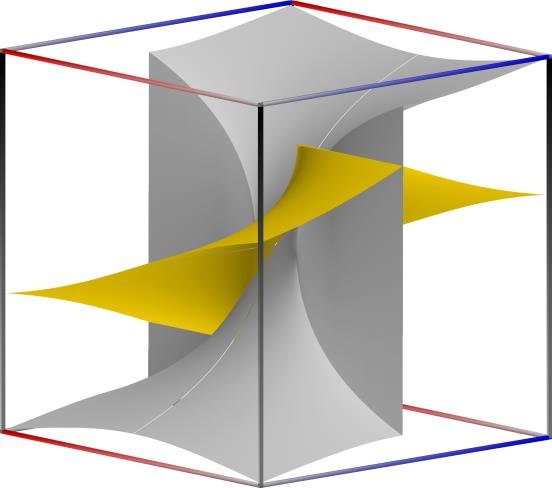
\includegraphics[height=8cm, width=8cm]{Charts/jpg/CplxAsinhBoth.jpg} }}%
	\qquad
	\subfloat[Magnitude and phase (color-coded), $z_{\text{min}}=0$. Camera angles are $\theta = 35\degree$ and $\phi = -112\degree$.]{{\includegraphics[height=8cm, width=8cm]{Charts/jpg/CplxAsinhMag.jpg} }}%
	\caption[Complex Inverse Hyperbolic Sine]{Surface plots of $z = \text{asinh}(x + iy)$, $-3 \leq x \leq 3$ (blue axis), $-2 \pi \leq y \leq 2\pi$ (red axis), $z_{\text{min}} \leq z \leq 10$ (black axis). $z$ values are truncated at $\pm 10$. There is a branch cut along the negative real axis. Orthographic camera. See section \ref{Graphics: Surface plots of complex functions} for more information about charts for complex functions.} 
	\label{fig:Complex Inverse Hyperbolic Sine}%
\end{figure}




\newpage
\subsection{\texorpdfstring{$\text{Inverse Hyperbolic Cosine: acosh}(z)$}{acosh}}

\begin{mpFunctionsExtract}
	\mpWorksheetFunctionOneNotImplemented
	{ACOSH? mpNum? the value of the hyperbolic arc-cosine  of $x$ in radians.}
	{x? mpNum? A real number.}
\end{mpFunctionsExtract}

\vspace{0.6cm}


\begin{mpFunctionsExtract}
	\mpFunctionOne
	{acosh? mpNum? the inverse complex hyperbolic cosine of $z$}
	{z? mpNum? A complex number.}
\end{mpFunctionsExtract}

\vspace{0.3cm}
The function \textsf{cplxACosh$(z)$} returns the inverse complex hyperbolic cosine of $z$: 
\begin{equation}
	\text{arccosh}(z) = \pm i \text{ arccos}(z),
\end{equation}
where $\text{arccos}(z)$ is defined in section \ref{inverse complex cosine}

Computes the inverse hyperbolic cosine of $x$, $\cosh^{-1}(x)=\log(x+\sqrt{x+1}\sqrt{x-1})$.

\begin{figure}[ht]%
	\centering
	\subfloat[Real ("silver") and imaginary ("gold") component, $z_{\text{min}}=-10$. Camera angles are $\theta = 135\degree$ and $\phi = -12\degree$.]{{\includegraphics[height=8cm, width=8cm]{Charts/jpg/CplxAcoshBoth.jpg} }}%
	\qquad
	\subfloat[Magnitude and phase (color-coded), $z_{\text{min}}=0$. Camera angles are $\theta = 35\degree$ and $\phi = -112\degree$.]{{\includegraphics[height=8cm, width=8cm]{Charts/jpg/CplxAcoshMag.jpg} }}%
	\caption[Complex Inverse Hyperbolic Cosine]{Surface plots of $z = \text{acosh}(x + iy)$, $-3 \leq x \leq 3$ (blue axis), $-2 \pi \leq y \leq 2\pi$ (red axis), $z_{\text{min}} \leq z \leq 10$ (black axis). $z$ values are truncated at $\pm 10$. There is a branch cut along the negative real axis. Orthographic camera. See section \ref{Graphics: Surface plots of complex functions} for more information about charts for complex functions.} 
	\label{fig:Complex Inverse Hyperbolic Cosine}%
\end{figure}


\newpage
\subsection{\texorpdfstring{$\text{Inverse Hyperbolic Tangent: atanh}(z)$}{atanh}}

\begin{mpFunctionsExtract}
	\mpWorksheetFunctionOneNotImplemented
	{ATANH? mpNum? the value of the hyperbolic arc-tangent  of $x$ in radians.}
	{x? mpNum? A real number.}
\end{mpFunctionsExtract}


\vspace{0.6cm}


\begin{mpFunctionsExtract}
	\mpFunctionOne
	{atanh? mpNum? the inverse complex hyperbolic tangent of $z$}
	{z? mpNum? A complex number.}
\end{mpFunctionsExtract}

\vspace{0.3cm}
The function \textsf{cplxATanh$(z)$} returns the inverse complex hyperbolic tangent of $z$: 
\begin{equation}
	\text{arctanh}(z) = -i \text{ arctan}(z),
\end{equation}
where $\text{arctan}(z)$ is defined in section \ref{inverse complex tangent}

Computes the inverse hyperbolic tangent of $x$, $\tanh^{-1}(x)=\tfrac{1}{2} (\log(1+x) - \log(1+x))$.


\begin{figure}[ht]%
	\centering
	\subfloat[Real ("silver") and imaginary ("gold") component, $z_{\text{min}}=-10$. Camera angles are $\theta = 135\degree$ and $\phi = -12\degree$.]{{\includegraphics[height=8cm, width=8cm]{Charts/jpg/CplxAtanhBoth.jpg} }}%
	\qquad
	\subfloat[Magnitude and phase (color-coded), $z_{\text{min}}=0$. Camera angles are $\theta = 35\degree$ and $\phi = -112\degree$.]{{\includegraphics[height=8cm, width=8cm]{Charts/jpg/CplxAtanhMag.jpg} }}%
	\caption[Complex Inverse Hyperbolic Tangent]{Surface plots of $z = \text{atanh}(x + iy)$, $-3 \leq x \leq 3$ (blue axis), $-2 \pi \leq y \leq 2\pi$ (red axis), $z_{\text{min}} \leq z \leq 10$ (black axis). $z$ values are truncated at $\pm 10$. There is a branch cut along the negative real axis. Orthographic camera. See section \ref{Graphics: Surface plots of complex functions} for more information about charts for complex functions.} 
	\label{fig:Complex Inverse Hyperbolic Tangent}%
\end{figure}



\newpage
\subsection{\texorpdfstring{$\text{Inverse Hyperbolic Cotangent: acoth}(z)$}{acoth}}
\label{inverse complex hyperbolic cotangent}

\begin{mpFunctionsExtract}
	\mpWorksheetFunctionOneNotImplemented
	{ACOTH? mpNum? the value of the hyperbolic arc-cotangent  of $x$ in radians.}
	{x? mpNum? A real number.}
\end{mpFunctionsExtract}

\vspace{0.6cm}



\begin{mpFunctionsExtract}
	\mpFunctionOne
	{acoth? mpNum? the inverse complex hyperbolic cotangent of $z$}
	{z? mpNum? A complex number.}
\end{mpFunctionsExtract}

\vspace{0.3cm}
The function \textsf{cplxACoth$(z)$} returns the inverse complex hyperbolic cotangent of $z$: 
\begin{equation}
	\text{arctanh}(z) = i \text{ arctan}(iz),
\end{equation}
where $\text{arctan}(z)$ is defined in section \ref{inverse complex cotangent}



Computes the inverse hyperbolic cotangent of $x$, $\text{coth}^{-1}(x) = \tanh^{-1}(1/x)$

\begin{figure}[ht]%
	\centering
	\subfloat[Real ("silver") and imaginary ("gold") component, $z_{\text{min}}=-10$. Camera angles are $\theta = 135\degree$ and $\phi = -12\degree$.]{{\includegraphics[height=8cm, width=8cm]{Charts/jpg/CplxAcothBoth.jpg} }}%
	\qquad
	\subfloat[Magnitude and phase (color-coded), $z_{\text{min}}=0$. Camera angles are $\theta = 35\degree$ and $\phi = -112\degree$.]{{\includegraphics[height=8cm, width=8cm]{Charts/jpg/CplxAcothMag.jpg} }}%
	\caption[Complex Inverse Hyperbolic Cotangent]{Surface plots of $z = \text{acoth}(x + iy)$, $-3 \leq x \leq 3$ (blue axis), $-2 \pi \leq y \leq 2\pi$ (red axis), $z_{\text{min}} \leq z \leq 10$ (black axis). $z$ values are truncated at $\pm 10$. There is a branch cut along the negative real axis. Orthographic camera. See section \ref{Graphics: Surface plots of complex functions} for more information about charts for complex functions.} 
	\label{fig:Complex Inverse Hyperbolic Cotangent}%
\end{figure}



\subsection{asech(x)}
Computes the inverse hyperbolic secant of $x$, $\text{sech}^{-1}(x) = \cosh^{-1}(1/x)$



\subsection{acsch(x)}
Computes the inverse hyperbolic cosecant of $x$, $\text{csch}^{-1}(x) = \sinh^{-1}(1/x)$




\newpage
\section{Elementary Functions of Mathematical Physics}

\subsection{\texorpdfstring{$\text{Bessel Function }J_{\nu}(x)$}{Bessel Function Jnu}}
\nomenclature{$J_{\nu}(z)$}{Bessel function of the first kind of real order $\nu$}

\label{BESSELJnu} 
\begin{mpFunctionsExtract}
	\mpWorksheetFunctionTwoNotImplemented
	{BESSELJ? mpNum? $J_{\nu}(z)$, the Bessel function of the first kind of real order $\nu$.}
	{x? mpNum? A real number.}
	{$\nu$? mpNum? A real number.}
\end{mpFunctionsExtract}

\vspace{0.3cm}
$J_{\nu}(z)$, the Bessel function of the first kind of order $\nu$, is defined as
\begin{equation}
	J_{\nu}(x)  = \left(\tfrac{1}{2}x\right)^{\nu}  \sum_{k=0}^\infty (-1)^k \frac{(x^2 / 4)^k}{k! \Gamma(\nu+k+1)}
\end{equation}




\subsection{\texorpdfstring{$\text{Bessel Function }Y_{\nu}(x)$}{Ynux}}
\nomenclature{$Y_{\nu}(z)$}{Bessel function of the second kind of real order $\nu$}
\label{BESSELYnu} 

\begin{mpFunctionsExtract}
	\mpWorksheetFunctionTwoNotImplemented
	{BESSELY? mpNum? $Y_{\nu}(z)$, the Bessel function of the second kind of order $\nu$.}
	{x? mpNum? A real number.}
	{$\nu$? mpNum? A real number.}
\end{mpFunctionsExtract}

\vspace{0.3cm}
$Y_{\nu}(z)$, the Bessel function of the second kind of order $\nu$, is defined as
\begin{equation}
	Y_{\nu}(x)  = \frac{J_{\nu}(x) \cos(\nu \pi) - J_{-\nu}(x)}{ \sin(\nu \pi)}
\end{equation}



\subsection{\texorpdfstring{$\text{Bessel Function }I_{\nu}(x)$}{Bessel Function Inu}}
\nomenclature{$I_{\nu}(z)$}{Modified Bessel function of the first kind of real order $\nu$}
\label{BESSELInu} 

\begin{mpFunctionsExtract}
	\mpWorksheetFunctionTwoNotImplemented
	{BESSELI? mpNum? $J_{\nu}(z)$, the Bessel function of the first kind of real order $\nu$.}
	{x? mpNum? A real number.}
	{$\nu$? mpNum? A real number.}
\end{mpFunctionsExtract}

\vspace{0.3cm}
This function returns the modified Bessel function $I_{\nu}(z)$ of the first kind of order $\nu$, defined as
\begin{equation}
	I_{\nu}(z)  = \frac{z}{2}  \sum_{j=0}^\infty \frac{(z^2 / 4)^j}{j! \Gamma(\nu+j+1)}
\end{equation}




\subsection{\texorpdfstring{$\text{Bessel Function }K_{\nu}(x)$}{Bessel Function Knu}}
\nomenclature{$K_{\nu}(z)$}{Modified Bessel function of the second kind of real order $\nu$}
\label{BESSELKnu} 

\begin{mpFunctionsExtract}
	\mpWorksheetFunctionTwoNotImplemented
	{BESSELK? mpNum?  $K_{\nu}(x)$, the modified Bessel function of the second kind of order $\nu$.}
	{x? mpNum? A real number.}
	{$\nu$? mpNum? A real number.}
\end{mpFunctionsExtract}

\vspace{0.3cm}
This function returns $K_{\nu}(z)$, the modified Bessel function of the second kind of order $\nu$, defined as
\begin{equation}
	K_{\nu}(x)  = \frac{\pi}{2} \frac{I_{-\nu}(x)) - I_{\nu}(x)}{ \sin(\nu \pi)}
\end{equation}




\vspace{0.6cm}
\begin{mpFunctionsExtract}
	\mpWorksheetFunctionOneNotImplemented
	{ERF? mpNum? the value of the error function.}
	{x? mpNum? A real number.}
\end{mpFunctionsExtract}

\vspace{0.6cm}
\begin{mpFunctionsExtract}
	\mpWorksheetFunctionOneNotImplemented
	{ERF.PRECISE? mpNum? the value of the error function.}
	{x? mpNum? A real number.}
\end{mpFunctionsExtract}

\vspace{0.3cm}
The error function is defined by
\begin{equation}
	\text{erf}(x) = \frac{2}{\sqrt{\pi}} \int_0^x e^{-x^2} dt,
\end{equation}



\subsection{Complementary Error Function}
\label{Complementary Error Function}

\vspace{0.6cm}
\begin{mpFunctionsExtract}
	\mpWorksheetFunctionOneNotImplemented
	{ERFC? mpNum? the value of the complementary error function.}
	{x? mpNum? A real number.}
\end{mpFunctionsExtract}

\vspace{0.6cm}
\begin{mpFunctionsExtract}
	\mpWorksheetFunctionOneNotImplemented
	{ERFC.PRECISE? mpNum? the value of the complementary error function.}
	{x? mpNum? A real number.}
\end{mpFunctionsExtract}

\vspace{0.3cm}
The complementary error function is defined by
\begin{equation}
	\text{erfc}(x) = 1-\text{erf}(x) = \frac{2}{\sqrt{\pi}} \int_x^\infty e^{-x^2} dt,
\end{equation}




\subsection{\texorpdfstring{$\text{Gamma function }\Gamma(x)$}{TGamma}}
\nomenclature{$\Gamma(x)$}{Gamma Function}
\label{GammaFunction}

\vspace{0.6cm}
\begin{mpFunctionsExtract}
	\mpWorksheetFunctionOneNotImplemented
	{GAMMA? mpNum? the gamma function for $x \neq 0, -1, -2,\ldots$.}
	{x? mpNum? A real number.}
\end{mpFunctionsExtract}

\vspace{0.3cm}
The gamma function for $x \neq 0, -1, -2,\ldots$ is defined by
\begin{equation}
	\Gamma(x)  = \int_{0}^{\infty} t^{x-1} e^{-t} dt \quad (x>0),
\end{equation}
and by analytic continuation if $x<0$, using the reflection formula
\begin{equation}
	\Gamma(x) \Gamma(1-x)  = \pi / \sin(\pi x).
\end{equation}



%\begin{mpFunctionsExtract}
	
	\begin{mpFunctionsExtract}
		\mpWorksheetFunctionOneNotImplemented
		{GAMMALN? mpNum? the logarithm of the gamma function.}
		{x? mpNum? A real number.}
	\end{mpFunctionsExtract}
	
	\vspace{0.6cm}
	
	\begin{mpFunctionsExtract}
		\mpWorksheetFunctionOneNotImplemented
		{GAMMALN.PRECISE? mpNum? the logarithm of the gamma function.}
		{x? mpNum? A real number.}
	\end{mpFunctionsExtract}
	
	
	
	\subsection{Beta Function B(a,b)}
	\label{BetaFunction}
	\begin{mpFunctionsExtract}
		\mpFunctionTwoNotImplemented
		{Beta? mpNum? the Beta function.}
		{a? mpNum? A real number.}
		{b? mpNum? A real number.}
	\end{mpFunctionsExtract}
	
	\vspace{0.3cm}
	This function computes $B(a,b)$ for $a, b \neq 0, -1, -2, \ldots$. 
	
	
	

\newpage
\section{Factorial and Related Functions}
\label{NumbertheoreticFunctions}
\subsection{Factorial}


\vspace{0.6cm}
\begin{mpFunctionsExtract}
	\mpWorksheetFunctionOneNotImplemented
	{FACT? Integer?  $n!$, the factorial of $n$}
	{n? Integer? An Integer.}
\end{mpFunctionsExtract}



\subsection{Double Factorial}

\begin{mpFunctionsExtract}
	\mpWorksheetFunctionOneNotImplemented
	{FACTDOUBLE? Integer?  $n!!$, the double factorial of $n$}
	{n? Integer? An Integer.}
\end{mpFunctionsExtract}




\subsection{Binomial Coefficient, Combinations}


\vspace{0.6cm}
\begin{mpFunctionsExtract}
	\mpWorksheetFunctionTwoNotImplemented
	{COMBIN? Integer? the binomial coefficient}
	{n? Integer? An Integer.}
	{k? Integer? An Integer.}
\end{mpFunctionsExtract}

\vspace{0.3cm}
Returns the binomial coefficient, $\binom{n}{k}$. Negative values of $n$ are supported, using the identity
\begin{equation}
	\binom{-n}{k} = (-1)^k \binom{n+k-1}{k}.
\end{equation}


\vspace{0.6cm}
\begin{mpFunctionsExtract}
	\mpWorksheetFunctionTwoNotImplemented
	{COMBINA? Integer? the binomial coefficient}
	{n? Integer? An Integer.}
	{k? Integer? An Integer.}
\end{mpFunctionsExtract}




\subsection{Multinomial}

\begin{mpFunctionsExtract}
	\mpWorksheetFunctionOneNotImplemented
	{MULTINOMIAL? mpReal? the multinomial}
	{a[]? mpReal? An array of integers.}
\end{mpFunctionsExtract}

\vspace{0.3cm}
Returns the multinomial, defined as  the ratio of the factorial of a sum of values to the product of factorials:
\begin{equation}
	\textsf{MULTINOMIAL}(a_1,a_2,\ldots,a_n) = \frac{(a_1+a_2+\ldots+a_n)!}{a_1! a_2! \ldots a_n!}
\end{equation}





\subsection{Permutations}

\begin{mpFunctionsExtract}
	\mpWorksheetFunctionTwoNotImplemented
	{PERMUT? Integer? the number of permutations for a given number $k$ of objects that can be selected from $n$ objects.}
	{n? Integer? An Integer.}
	{k? Integer? An Integer.}
\end{mpFunctionsExtract}

\vspace{0.3cm}
\begin{mpFunctionsExtract}
	\mpWorksheetFunctionTwoNotImplemented
	{PERMUTATIONA? Integer? the number of permutations for a given number $k$ of objects that can be selected from $n$ objects.}
	{n? Integer? An Integer.}
	{k? Integer? An Integer.}
\end{mpFunctionsExtract}

\vspace{0.3cm}
Returns the number of permutations for a given number $k$ of objects that can be selected from $n$ objects. A permutation is any set or subset of objects or events where internal order is significant.
\begin{equation}
	\textsf{PERMUT}(n, k) = \frac{n!}{(n-k)!}
\end{equation}



\subsection{Greatest Common Divisor (GCD)}


\vspace{0.6cm}
\begin{mpFunctionsExtract}
	\mpWorksheetFunctionTwoNotImplemented
	{GCD? Integer? the greatest common divisor of $n_1$ and $n_2$}
	{n1? Integer? An Integer.}
	{n2? Integer? An Integer.}
\end{mpFunctionsExtract}

\vspace{0.3cm}
The result is always positive even if
one or both input operands are negative. Except if both inputs are zero; then this function
defines \textsf{intGcd}(0, 0) = 0.



\subsection{Least Common Multiple (LCM)}


\vspace{0.6cm}
\begin{mpFunctionsExtract}
	\mpWorksheetFunctionTwoNotImplemented
	{LCM? Integer? the least common multiple of $n_1$ and $n_2$.}
	{n1? Integer? An Integer.}
	{n2? Integer? An Integer.}
\end{mpFunctionsExtract}

\vspace{0.3cm}
Returns the least common multiple of $n_1$ and $n_2$. The returned value is always positive, irrespective of the signs of $n_1$ and $n_2$. The returned value  will be zero if either $n_1$ or $n_2$ is zero.




\chapter{Linear Algebra}

\section{Multiple Linear Regression}



\subsection{Determinant}

\begin{mpFunctionsExtract}
	\mpWorksheetFunctionOneNotImplemented
	{MDETERM? mpNum? the matrix determinant of a numeric array $X$ with an equal number of rows and columns.}
	{X? mpNum[]? A matrix of real numbers.}
\end{mpFunctionsExtract}





\subsection{Inverse}

\begin{mpFunctionsExtract}
	\mpWorksheetFunctionOneNotImplemented
	{MINVERSE? mpNum? the  inverse matrix for the matrix stored in the numeric array  $X$ with an equal number of rows and columns.}
	{X? mpNum[]? A matrix of real numbers.}
\end{mpFunctionsExtract}


Negative powers will calculate the inverse:

\lstset{language={Python}}
\begin{lstlisting}
>>> A**-1
matrix(
[['-2.0', '1.0'],
['1.5', '-0.5']])
>>> nprint(A * A**-1, 3)
[ 1.0 1.08e-19]
[-2.17e-19 1.0]
\end{lstlisting}






\subsection{LinEst}
\label{LinEst}

\begin{mpFunctionsExtract}
	\mpWorksheetFunctionFourNotImplemented
	{LINEST? mpNumList? information obtained by performing multiple liner regression.}
	{Y? mpNum[]? An array of real numbers.}
	{X? mpNum[]? An array of real numbers.}
	{Const? Boolean? A logical value.}
	{Stats? Boolean? A logical value.}
\end{mpFunctionsExtract}



\vspace{0.3cm}
The LINEST function calculates the statistics for a line by using the "least squares" method to calculate a straight line that best fits your data, and then returns an array that describes the line. 

You can also combine LINEST with other functions to calculate the statistics for other types of models that are linear in the unknown parameters, including polynomial, logarithmic, exponential, and power series. Because this function returns an array of values, it must be entered as an array formula. Instructions follow the examples in this article.

This function can also be used to perform multiple linear regression.

This function needs a detailed explanation.



\subsection{TREND}

\begin{mpFunctionsExtract}
	\mpWorksheetFunctionFourNotImplemented
	{TREND? mpNumList? values along a linear trend.}
	{Y? mpNum[]? An array of real numbers.}
	{X? mpNum[]? An array of real numbers.}
	{NewX? mpNum[]? An array of real numbers.}
	{Const? Boolean? A logical value.}
\end{mpFunctionsExtract}

\vspace{0.3cm}
Returns values along a linear trend. Fits a straight line (using the method of least squares) to the arrays $Y$ and $X$. Returns the y-values along that line for the array of $NewX$ that you specify.

For information about how Microsoft Excel fits a line to data, see LINEST.
You can use TREND for polynomial curve fitting by regressing against the same variable raised to different powers. For example, suppose column A contains y-values and column B contains x-values. You can enter $x^2$ in column C, $x^3$ in column D, and so on, and then regress columns B through D against column A.

Formulas that return arrays must be entered as array formulas.



\newpage
\section{Exponential Growth Curves}

\subsection{LogEst}

\begin{mpFunctionsExtract}
	\mpWorksheetFunctionFourNotImplemented
	{LOGEST? mpNumList? an exponential curve that fits your data and returns an array of values that describes the curve.}
	{Y? mpNum[]? An array of real numbers.}
	{X? mpNum[]? An array of real numbers.}
	{Const? Boolean? A logical value.}
	{Stats? Boolean? A logical value.}
\end{mpFunctionsExtract}

\vspace{0.3cm}
In regression analysis, calculates an exponential curve that fits your data and returns an array of values that describes the curve. Because this function returns an array of values, it must be entered as an array formula.

This function does not perform a non-linear estimation.



\subsection{Growth}

\begin{mpFunctionsExtract}
	\mpWorksheetFunctionFourNotImplemented
	{GROWTH? mpNumList? predicted exponential growth by using existing data.}
	{Y? mpNum[]? An array of real numbers.}
	{X? mpNum[]? An array of real numbers.}
	{NewX? mpNum[]? An array of real numbers.}
	{Const? Boolean? A logical value.}
\end{mpFunctionsExtract}

\vspace{0.3cm}
\textsf{GROWTH} returns the $y$-values for a series of new $x$-values that you specify by using existing $x$-values and $y$-values. You can also use the \textsf{GROWTH} worksheet function to fit an exponential curve to existing $x$-values and $y$-values.



\newpage
\section{Norms}
Sometimes you need to know how 'large' a matrix or vector is. Due to their multidimensional nature it is not possible to compare them, but there are several functions to map a matrix or a vector to a positive real number, the so called norms.

\vpara
\begin{mpFunctionsExtract}
	\mpFunctionTwo
	{norm? mpNumList? the entrywise $p$-norm of an iterable x, i.e. the vector norm.}
	{Y? mpNum[]? An array of real numbers.}
	{Keywords? String?  p=2.}
\end{mpFunctionsExtract}


norm(ctx, x, p=2)
Gives the entrywise $p$-norm of an iterable x, i.e. the vector norm 

\begin{equation}
	\left( \sum_k |x_k|^p \right)^{1/p},
\end{equation}
for any given $1 \leq p \leq \infty$.

Special cases:

If x is not iterable, this just returns absmax(x).

p=1 gives the sum of absolute values.

p=2 is the standard Euclidean vector norm.

p=inf gives the magnitude of the largest element.

For x a matrix, p=2 is the Frobenius norm. For operator matrix norms, use mnorm() instead.

You can use the string 'inf' as well as float('inf') or mpf('inf') to specify the infinity norm.

\vpara
\textbf{Examples}

\lstset{language={Python}}
\begin{lstlisting}
>>> from mpFormulaPy import *
>>> mp.dps = 15; mp.pretty = False
>>> x = matrix([-10, 2, 100])
>>> norm(x, 1)
mpf('112.0')
>>> norm(x, 2)
mpf('100.5186549850325')
>>> norm(x, inf)
mpf('100.0')
\end{lstlisting}


\vspace{0.6cm}

\begin{mpFunctionsExtract}
	\mpFunctionTwo
	{mnorm? mpNumList? the matrix (operator) $p$-norm of A. Currently p=1 and p=inf are supported.}
	{A? mpNum[]? An array of real numbers.}
	{Keywords? String?  p=1.}
\end{mpFunctionsExtract}


mnorm(ctx, A, p=1)

Gives the matrix (operator) $p$-norm of A. Currently p=1 and p=inf are supported:

p=1 gives the 1-norm (maximal column sum)

p=inf gives the -norm (maximal row sum). You can use the string 'inf' as well as float('inf') or mpf('inf')

p=2 (not implemented) for a square matrix is the usual spectral matrix norm, i.e. the largest singular value.

p='f' (or 'F', 'fro', 'Frobenius', 'frobenius') gives the Frobenius norm, which is the elementwise 2-norm. The Frobenius norm is an approximation of the spectral norm and satisfies

\begin{equation}
	\frac{1}{\sqrt{\text{rank}(A)}} ||A||_F \leq ||A||_2 \leq ||A||_F.
\end{equation}

The Frobenius norm lacks some mathematical properties that might be expected of a norm.

For general elementwise $p$-norms, use norm() instead.

\vpara
\textbf{Examples}

\lstset{language={Python}}
\begin{lstlisting}
>>> from mpFormulaPy import *
>>> mp.dps = 15; mp.pretty = False
>>> A = matrix([[1, -1000], [100, 50]])
>>> mnorm(A, 1)
mpf('1050.0')
>>> mnorm(A, inf)
mpf('1001.0')
>>> mnorm(A, 'F')
mpf('1006.2310867787777')
\end{lstlisting}





\newpage
\section{Decompositions}


\begin{mpFunctionsExtract}
	\mpFunctionTwo
	{cholesky? mpNum? the Cholesky decomposition of a symmetric positive-definite matrix $A$.}
	{A? mpNum[]? A symmetric matrix.}
	{Keywords? String?  tol=None.}
\end{mpFunctionsExtract}


cholesky(ctx, A, tol=None)

Cholesky decomposition of a symmetric positive-definite matrix $A$. Returns a lower triangular matrix $L$ such that $A=L \times L^T$. More generally, for a complex Hermitian positive-definite matrix, a Cholesky decomposition satisfying $A=L \times L^H$ is returned.

\vpara
The Cholesky decomposition can be used to solve linear equation systems twice as efficiently as LU decomposition, or to test whether $A$ is positive-definite.

\vpara
The optional parameter tol determines the tolerance for verifying positive-definiteness.

\vpara
\textbf{Examples}

Cholesky decomposition of a positive-definite symmetric matrix:

\lstset{language={Python}}
\begin{lstlisting}
>>> from mpFormulaPy import *
>>> mp.dps = 25; mp.pretty = True
>>> A = eye(3) + hilbert(3)
>>> nprint(A)
[ 2.0 0.5 0.333333]
[ 0.5 1.33333 0.25]
[0.333333 0.25 1.2]
>>> L = cholesky(A)
>>> nprint(L)
[ 1.41421 0.0 0.0]
[0.353553 1.09924 0.0]
[0.235702 0.15162 1.05899]
>>> chop(A - L*L.T)
[0.0 0.0 0.0]
[0.0 0.0 0.0]
[0.0 0.0 0.0]
\end{lstlisting}

Cholesky decomposition of a Hermitian matrix:

\lstset{language={Python}}
\begin{lstlisting}
>>> A = eye(3) + matrix([[0,0.25j,-0.5j],[-0.25j,0,0],[0.5j,0,0]]
>>> L = cholesky(A)
>>> nprint(L)
[ 1.0 0.0 0.0]
[(0.0 - 0.25j) (0.968246 + 0.0j) 0.0]
[ (0.0 + 0.5j) (0.129099 + 0.0j) (0.856349 + 0.0j)]
>>> chop(A - L*L.H)
[0.0 0.0 0.0]
[0.0 0.0 0.0]
[0.0 0.0 0.0]
\end{lstlisting}

Attempted Cholesky decomposition of a matrix that is not positive definite:

\lstset{language={Python}}
\begin{lstlisting}
>>> A = -eye(3) + hilbert(3)
>>> L = cholesky(A)
Traceback (most recent call last):
...
ValueError: matrix is not positive-definite
\end{lstlisting}




\newpage
\section{Linear Equations}


\begin{mpFunctionsExtract}
	\mpFunctionThree
	{lu\_solve? mpNum? solves a linear equation system using a LU decomposition.}
	{A? mpNum[]? A symmetric matrix.}
	{b? mpNum[]? A symmetric matrix.}	
	{Keywords? String?  tol=None.}
\end{mpFunctionsExtract}


You can for example solve the linear equation system using a LU decomposition:

\lstset{language={Python}}
\begin{lstlisting}
x + 2*y = -10
3*x + 4*y = 10
\end{lstlisting}

using lu\_solve:

\lstset{language={Python}}
\begin{lstlisting}
>>> A = matrix([[1, 2], [3, 4]])
>>> b = matrix([-10, 10])
>>> x = lu_solve(A, b)
>>> x
matrix(
[['30.0'],
['-20.0']])
\end{lstlisting}


\begin{mpFunctionsExtract}
	\mpFunctionFour
	{residual? mpNum? the residual  $||Ax-b||$.}
	{A? mpNum[]? A square matrix.}
	{b? mpNum[]? A vector.}
	{x? mpNum[]? A vector.}		
	{Keywords? String?  tol=None.}
\end{mpFunctionsExtract}


Calculates the residual  $||Ax-b||$:

\lstset{language={Python}}
\begin{lstlisting}
>>> residual(A, x, b)
matrix(
[['3.46944695195361e-18'],
['3.46944695195361e-18']])
>>> str(eps)
'2.22044604925031e-16'
\end{lstlisting}

As you can see, the solution is quite accurate. The error is caused by the inaccuracy of the internal floating point arithmetic. Though, it is even smaller than the current machine epsilon, which basically means you can trust the result.

If you need more speed, use NumPy, or use fp instead mp matrices and methods:

\lstset{language={Python}}
\begin{lstlisting}
>>> A = fp.matrix([[1, 2], [3, 4]])
>>> b = fp.matrix([-10, 10])
>>> fp.lu_solve(A, b)
matrix(
[['30.0'],
['-20.0']])
\end{lstlisting}

lu\_solve accepts overdetermined systems. It is usually not possible to solve such systems, so the residual is minimized instead. Internally this is done using Cholesky decomposition to compute a least squares approximation. This means that that lu\_solve will square the errors. If you cannot afford this, use qr\_solve instead. It is twice as slow but more accurate, and it calculates the residual automatically.



\newpage
\section{Matrix Factorization}

\begin{mpFunctionsExtract}
	\mpFunctionTwo
	{lu? mpNum? an explicit LU factorization of a matrix, returning P, L, U}
	{A? mpNum[]? A square matrix.}
	{Keywords? String?  tol=None.}
\end{mpFunctionsExtract}


The function lu computes an explicit LU factorization of a matrix:

\lstset{language={Python}}
\begin{lstlisting}
>>> P, L, U = lu(matrix([[0,2,3],[4,5,6],[7,8,9]]))
>>> print P
[0.0 0.0 1.0]
[1.0 0.0 0.0]
[0.0 1.0 0.0]
>>> print L
[ 1.0 0.0 0.0]
[ 0.0 1.0 0.0]
[0.571428571428571 0.214285714285714 1.0]
>>> print U
[7.0 8.0 9.0]
[0.0 2.0 3.0]
[0.0 0.0 0.214285714285714]
>>> print P.T*L*U
[0.0 2.0 3.0]
[4.0 5.0 6.0]
[7.0 8.0 9.0]
\end{lstlisting}




\begin{mpFunctionsExtract}
	\mpFunctionTwo
	{qr? mpNum? an explicit QR factorization of a matrix, returning Q, R}
	{A? mpNum[]? A square matrix.}
	{Keywords? String?  tol=None.}
\end{mpFunctionsExtract}

\vpara
Examples:

\lstset{language={Python}}
\begin{lstlisting}
>>> A = matrix([[1, 2], [3, 4], [1, 1]])
>>> Q, R = qr(A)
>>> print Q
[-0.301511344577764 0.861640436855329 0.408248290463863]
[-0.904534033733291 -0.123091490979333 -0.408248290463863]
[-0.301511344577764 -0.492365963917331 0.816496580927726]
>>> print R
[-3.3166247903554 -4.52267016866645]
[ 0.0 0.738548945875996]
[ 0.0 0.0]
>>> print Q * R
[1.0 2.0]
[3.0 4.0]
[1.0 1.0]
>>> print chop(Q.T * Q)
[1.0 0.0 0.0]
[0.0 1.0 0.0]
[0.0 0.0 1.0]
\end{lstlisting}






\newpage
\section{Time Series}
%\lipsum[1]

\subsection{Exponential Smoothing}
\label{Exponential Smoothing}
This section covers Exponential Smoothing, as implemented in Excel Toolpak


\subsection{Moving Average}
\label{Moving Average}
This section covers Moving Average, as implemented in Excel Toolpak





\chapter{Distribution Functions}

\section{Introduction to Distribution Functions}
\label{DistributionFunctionsIntroduction} 

%\lipsum[1]

This is a citation~\citet{walck_2007}, and some more.

This is a citation~\citet{VanHauwermeiren_2009}, and some more.

This is a citation~\citet{Rinne_book_2008}, and some more.

This is a citation~\citet{Johnson_1994}, and some more.

This is a citation~\citet{Johnson_1995}, and some more.
\nomenclature{pmf}{probability mass function}%
\nomenclature{pdf}{probability density function}%
\nomenclature{CDF}{cumulative distribution function}%


See also \cite{Monahan_2011}

See also \cite{Lange_2010}

See also \cite{Chernick_2008}

See also \cite{Cheney_2008}


\subsection{Continuous Distribution Functions}

Continuous random number distributions are defined by a probability density function, $p(x)$, such that the probability of $x$ occurring in the infinitesimal range $x$ to $x +dx$ is $p\ dx$. The cumulative distribution function for the lower tail $P(x)$ gives the probability of a variate taking a value less than $x$, and the cumulative distribution function for the upper tail $Q(x)$ gives the probability of a variate taking a value greater than $x$. 

The upper and lower cumulative distribution functions are related by $P(x) + Q(x) = 1$ and satisfy $0 \leq P(x) \leq 1, 0 \leq Q(x) \leq 1$. The inverse cumulative distributions, $x = P-1(P)$ and $x = Q-1(Q)$ give the values of $x$ which correspond to a specific value of $P$ or $Q$. They can be used to find confidence limits from probability values. 



\subsection{Discrete Distribution Functions}

For discrete distributions the probability of sampling the integer value $k$ is given by $p(k)$. The cumulative distribution for the lower tail $P(k)$ of a discrete distribution is defined as the sum over the allowed range of the distribution less than or equal to $k$. The cumulative distribution for the upper tail of a discrete distribution $Q(k)$ is defined as the sum of probabilities for all values greater than $k$. These two definitions satisfy the identity $P(k) + Q(k) = 1$. If the range of the distribution is 1 to $n$ inclusive then $P(n) = 1$, $Q(n) = 0$ while $P(1) = p(1)$, $Q(1) = 1 - p(1)$. 


\newpage
\subsection{Commonly Used Function Types}
\label{Commonly Used Distribution Function Types}

\subsubsection{Functions returning pdf, CDF, and related information}
\label{Functions returning pdf, CDF, and related information}
These functions have the form \textsf{?Dist($x$; [Parameters;], OutputString)}.
Here 

"?" is a placeholder for the name of the distribution, 

"$x$" is the value for which we want to calculate the pdf, CDF etc, 

"[Parameters;]" denote any parameters (like degrees of freedom) of the distribution, and 

"OutputString" specifies the computed results which will be returned. This can be any of the following:

\begin{itemize}
	\item \textbf{pdf}: the probability density function
	\item \textbf{P}: the cumulative distribution function (CDF)
	\item \textbf{Q}: the complement of cumulative distribution function (CDF)
	\item \textbf{logpdf}: the logarithm of the probability density function
	\item \textbf{logP}: the logarithm of the cumulative distribution function (CDF)
	\item \textbf{logQ}: the logarithm of the complement of cumulative distribution function (CDF)
	\item \textbf{h}: hazard function
	\item \textbf{H}: cumulative hazard function
\end{itemize}


\vspace{0.3cm}
As an example, for Student's t-distribution, a "T" is used to specify the name of the distibution, and there is just one distribution parameter, $\nu$, the degrees of freedom. Therefore,  the function has the form

\vspace{0.3cm}
\textsf{TDist($x$ As nmNum; $\nu$ As mpNum, OutputString As String) As mpNumList}, 

\vspace{0.3cm}
and an actual call to the function, requesting the pdf, CDF, and the complement of the CDF for $x=2.3$ and $\nu=22$ could be

\lstset{language={[Visual]Basic}}
\begin{lstlisting}
Result = TDist(2.3, 22, "pdf + P + Q")
mp.Print Result
\end{lstlisting}
which produces the output

\begin{verbatim}
pdf: 0.434234342343434
P: 0.943453463453453
Q: 0.054564564564236
\end{verbatim}




\newpage
\subsubsection{Functions returning Quantiles}
\label{Functions returning Quantiles}
These functions have the form \textsf{?DistInv(Prob; [Parameters;], OutputString)}.
Here 

"?" is a placeholder for the name of the distribution, 

"Prob" sets the target values for $P$ and $Q$, 

"[Parameters;]" denote any parameters (like degrees of freedom) of the distribution, and 

"OutputString" specifies the computed results which will be returned. This can be any of the following:

\begin{itemize}
	\item \textbf{PInv}: the inverse of the cumulative distribution function (CDF). For discrete distribution, this will be outwardly rounded
	\item \textbf{QInv}: the inverse of the complement of the cumulative distribution function (CDF). For discrete distribution, this will be outwardly rounded
	\item \textbf{P}: the value of the cumulative distribution function (CDF), which has actually been achieved
	\item \textbf{Q}: the value of the complement of the cumulative distribution function (CDF), which has actually been achieved
\end{itemize}


\vspace{0.3cm}
As an example, for Student's t-distribution, a "T" is used to specify the name of the distibution, and there is just one distribution parameter, $\nu$, the degrees of freedom. Therefore,  the function has the form

\vspace{0.3cm}
\textsf{TDistInv($Prob$ As mpNum; $\nu$ As mpNum, OutputString As String) As mpNumList}, 

\vspace{0.3cm}
and an actual call to the function, requesting the inverse of the complement of the CDF for $Prob=0.01$ and $\nu=22$ could be

\lstset{language={[Visual]Basic}}
\begin{lstlisting}
Result = TDistInv(0,01, 22, "QInv")
mp.Print Result
\end{lstlisting}
which produces the output

\begin{verbatim}
QInv: 2.943453463453453
\end{verbatim}


\newpage
\subsubsection{Functions returning moments and related information}
\label{Functions returning moments and related information}
These functions have the form \textsf{?DistInfo([Parameters;], OutputString)}.
Here 

"?" is a placeholder for the name of the distribution, 

"[Parameters;]" denote any parameters (like degrees of freedom) of the distribution, and 

"OutputString" specifies the computed results which will be returned. This can be any of the following:

\begin{itemize}
	\item \textbf{range}: Returns the valid range of the random variable over distribution dist. 
	\item \textbf{support}: 	
	\item \textbf{mode}: Returns the mode of the distribution dist. This function may return a domain\_error if the distribution does not have a defined mode.
	\item \textbf{median}: Returns the median of the distribution dist.
	\item \textbf{mean}: Returns the mean of the distribution dist. This function may return a domain\_error if the distribution does not have a defi ned mean (for e xample the Cauchy distribution).
	\item \textbf{stdev}: Returns the standard deviation of distribution dist.
	This function may return a domain\_error if the distribution does not have a defined standard deviation.
	\item \textbf{variance}: Returns the variance of the distribution dist.
	This function may return a domain\_error if the distribution does not have a defi ned v ariance.
	\item \textbf{skewness}: Returns the skewness of the distribution dist.
	This function may return a domain\_error if the distribution does not have a defined skewness.
	\item \textbf{kurtosis}: Returns the 'proper' kurtosis (normalized fourth moment) of the distribution dist.
	\item \textbf{kurtosis excess}: Returns the kurtosis excess of the distribution dist. kurtosis excess = kurtosis - 3
\end{itemize}



\vspace{0.3cm}
As an example, for Student's t-distribution, a "T" is used to specify the name of the distibution, and there is just one distribution parameter, $\nu$, the degrees of freedom. Therefore,  the function has the form

\vspace{0.3cm}
\textsf{TDistInfo($\nu$ As mpNum, OutputString As String) As mpNumList}, 

\vspace{0.3cm}
and an actual call to the function, requesting the mean, varaince, skewness and kurtosis with $\nu=22$ could be

\lstset{language={[Visual]Basic}}
\begin{lstlisting}
Result = TDistInfo(22, "mean + variance + skewness + kurtosis")
mp.Print Result
\end{lstlisting}
which produces the output

\begin{verbatim}
mean: 0.434234342343434
variance: 0.943453463453453
skewness: 0.054564564564236
kurtosis: 0.6054564564564236
\end{verbatim}









\newpage
\subsubsection{Functions returning Sample Size estimates}
\label{Functions returning Sample Size estimates}
These functions have the form \textsf{?SampleSize(Alpha; Beta; ModifiedNoncentrality; [Parameters;],  OutputString)}.
Here 

"?" is a placeholder for the name of the distribution, 

"Alpha" specifies the confidence level (or Type I error), 

"Beta" specifies the Type I error (or 1 $-$ Power), 

"ModifiedNoncentrality" specifies the (modified) noncentrality parameter of the distribution in a form which does not depend on sample size (which may require a modification compared to the conventional form for stating the noncentrlaity parameter), 

"[Parameters;]" denote any additional parameters of the distribution (if any) which are not a function of the sample size, and 

"OutputString" specifies the computed results which will be returned. This can be any of the following:

\begin{itemize}
	\item \textbf{ExactN}: returns an "exact", i.e. typically non-integer sample size estimate 
	\item \textbf{UpperN}: upper integer sample size estimate
	\item \textbf{LowerN}: lower integer sample size estimate
	\item \textbf{UpperNPower}: actual power when using UpperN
	\item \textbf{LowerNPower}: actual power when using LowerN
\end{itemize}


\vspace{0.3cm}
As an example, for the noncentral  t-distribution, the prefix "NoncentralT" is used to specify the name of the distibution. The distribution parameter $\nu$, the degrees of freedom, which depends on the sample size, and is therefore not included in the parameter list of this function. The modified noncentrality parameter is called $\tilde{\rho} = \Delta/\sigma$. Therefore, the function has the form

\vspace{0.3cm}
\textsf{NoncentralTSampleSize($\alpha$ As mpNum, $\beta$ As mpNum, $\tilde{\rho}$ As mpNum, OutputString As String) As mpNumList}

\vspace{0.3cm}
and an actual call to the function, requesting an upper sample size estimate (and actual power) for $\alpha = 0.95$, $\beta=0.1$ , and $\tilde{\rho} = \Delta/\sigma = 0.6$   would be

\lstset{language={[Visual]Basic}}
\begin{lstlisting}
Result = NoncentralTSampleSize(0.95, 0.1, 0.6, "UpperN + UpperNPower")
mp.Print Result
\end{lstlisting}
which produces the output

\begin{verbatim}
UpperN: 26
UpperNPower: 0.92435435
\end{verbatim}



\newpage
\subsubsection{Functions related to noncentrality parameters}
\label{Functions related to noncentrality parameters}
These functions have the form \textsf{?Noncentrality(Alpha; Noncentrality; [Parameters;],  OutputString)}.
Here 

"?" is a placeholder for the name of the distribution, 

"Alpha" specifies the confidence level (or Type I error), 

"Noncentrality" specifies the noncentrality parameter of the distribution, 

"[Parameters;]" denote any additional parameters of the distribution, and 

"OutputString" specifies the computed results which will be returned. This can be any of the following:

\begin{itemize}
	\item \textbf{UpperCI}: upper confidence interval
	\item \textbf{LowerCI}: lower confidence interval
	\item \textbf{TwoSidedCI}: two-sided confidence interval
\end{itemize}


\vspace{0.3cm}
As an example, for the noncentral  t-distribution, the prefix "NoncentralT" is used to specify the name of the distibution. The noncentrality parameter is $\delta$, and the other distribution parameter is $\nu$, the degrees of freedom.  Therefore, the function has the form

\vspace{0.3cm}
\textsf{NoncentralTNoncentrality($\alpha$ As mpNum, $\delta$ As mpNum, $\nu$ As mpNum, OutputString As String) As mpNumList}

\vspace{0.3cm}
and an actual call to the function, requesting an upper confidence interval for $\delta$ with $\alpha = 0.95$, $\delta = 0.6$ and $\nu=22$   would be

\lstset{language={[Visual]Basic}}
\begin{lstlisting}
Result = NoncentralTNoncentrality(0.95, 0.6, 22, "UpperCI")
mp.Print Result
\end{lstlisting}
which produces the output

\begin{verbatim}
UpperCI: 0.7546534
\end{verbatim}



\newpage
\subsubsection{Functions returning Random numbers}
\label{Functions returning Random numbers}
These functions have the form \textsf{?DistRan(Size; [Parameters;], Generator, OutputString)}.
Here 

"?" is a placeholder for the name of the distribution, 

"Size" specifies the size of the random sample, 

"[Parameters;]" denote any parameters (like degrees of freedom) of the distribution, and 

"Generator" specifies the pseudo random generator which will be used to produce the random sample, 

"OutputString" specifies the computed results which will be returned. This can be any of the following:

\begin{itemize}
	\item \textbf{Unsorted}: produces unsorted output
	\item \textbf{Ascending}: output sorted in ascending order
	\item \textbf{Descending}: output sorted in descending order
	\item \textbf{Histogram($k$)}: output grouped in histogram format, with $k$ buckets
	\item \textbf{HistogramCDF($k$)}: cumulated output grouped in histogram format, with $k$ buckets
	
\end{itemize}


\vspace{0.3cm}
As an example, for Student's t-distribution, a "T" is used to specify the name of the distibution, and there is just one distribution parameter, $\nu$, the degrees of freedom. Therefore,  the function has the form

\vspace{0.3cm}
\textsf{TDistRan($Size$ As Integer; $\nu$ As mpNum, Generator As String, OutputString As String) As mpNumList}, 

\vspace{0.3cm}
and an actual call to the function, requesting a random sample of  $Size=10000$ of a t-distribution with $\nu=22$, using the default pseudo-random number generator, sorting output in ascending order could be

\lstset{language={[Visual]Basic}}
\begin{lstlisting}
Result = TDistRan(10000, 22, "Default", "Ascending")
mp.Plot Result
\end{lstlisting}
which produces the output

\begin{verbatim}
QInv: 2.943453463453453
\end{verbatim}



\newpage
\section{Beta-Distribution}
\label{BetaDistribution}

\subsection{Definition}
\label{BetaDistributionDefinition}

If $X_1$ an $X_2$ is are independent random variables  following  $\chi^2$-distribution with $2a$ and $2b$ degrees of freedom respectively, 
then the distribution of the ratio $\frac{X_1}{X_1+X_2}$ is said to follow a Beta-distribution with  $a$ and $b$  degrees of freedom.

See \cite{Tretter_1979}


\subsection{Density and CDF}

\begin{mpFunctionsExtract}
	\mpFunctionFourNotImplemented
	{BetaDist? mpNumList? pdf, CDF and related information for the central Beta-distribution}
	{x? mpNum? A real number}
	{a? mpNum? A real number greater 0, representing the numerator  degrees of freedom}
	{b? mpNum? A real number greater 0, representing the denominator degrees of freedom}
	{Output? String? A string describing the output choices}
\end{mpFunctionsExtract}


\vspace{0.3cm}
See section \ref{Functions returning pdf, CDF, and related information} for the options for {\itshape\sffamily Output}. Algorithms and formulas are given in sections \ref{BetaDistributionDensity} and \ref{BetaDistributionCDF}.


\vspace{0.3cm}

The following functions are provided for compatibility with established spreadsheet functions

\vspace{0.3cm}
\begin{mpFunctionsExtract}
	\mpWorksheetFunctionThreeNotImplemented
	{BETADIST? mpReal? the CDF and of the central Beta-distribution}
	{x? mpReal? A real number. The numeric value at which to evaluate the distribution}
	{a? mpNum? A real number greater 0, representing the numerator  degrees of freedom}
	{b? mpNum? A real number greater 0, representing the denominator degrees of freedom}
\end{mpFunctionsExtract}

\vspace{0.6cm}
\begin{mpFunctionsExtract}
	\mpWorksheetFunctionFourNotImplemented
	{BETA.DIST? mpReal? the CDF and of the central Beta-distribution}
	{x? mpReal? A real number. The numeric value at which to evaluate the distribution}
	{a? mpNum? A real number greater 0, representing the numerator  degrees of freedom}
	{b? mpNum? A real number greater 0, representing the denominator degrees of freedom}
	{Cumulative ? Boolean? A logical value that determines the form of the function. If cumulative is TRUE, T.DIST returns the cumulative distribution function; if FALSE, it returns the probability density function}
\end{mpFunctionsExtract}


\subsubsection{Density}
\nomenclature{$f_{\text{Beta}}(a,b,x)$}{pdf of the central Beta-distribution}
\label{BetaDistributionDensity}
The pdf of a variable following a central  Beta-distribution with $a$ and $b$ degrees of freedom is given by

\begin{equation}
	f_{\text{Beta}}(a,b,x) = \frac{1}{B(a,b)} x^{a-1}(1-x)^{b-1}
\end{equation}
where $B(a,b)$ denotes the beta function (see section \ref{BetaFunction}).

\subsubsection{CDF: General formulas}
\nomenclature{$F_{\text{Beta}}(a,b,x)$}{CDF of the central Beta-distribution}
\label{BetaDistributionCDF}
The cdf of a variable following a central  Beta-distribution with $a$ and $b$ degrees of freedom is given by

\begin{equation}
	\text{Pr}\left[X \le x\right] = F_{\text{Beta}}\left(a,b,x\right) =  \int_{0}^{x} f_{\text{Beta}}(a,b,t) dt
\end{equation}

\subsubsection{Exact cdf as continued fraction}
The following representation as continued fraction is used (Peizer 1968, .1428 and 1452):
\begin{equation}
	I(a,b,x)= \binom{n}{a} p^{b-1} q^a \frac{1}{(1+u_1/(v_1+u_2/(v2+u3/(v_3+ \cdots))))}, \quad \text{where } 
\end{equation}
\begin{equation*}
	p=(1-x), \quad q=x, \quad n=a+b-1, \quad u_1= \frac{-(b-1)q}{p}, \quad u_{2j}= \frac{j(n+j)q}{p},
\end{equation*}
\begin{equation*}
	u_{2j+1}= \frac{-(a+j)(b-j-1)q}{p}, \quad v_j=a+j, \quad j=1,2,\ldots
\end{equation*}


\subsection{Quantiles}

\begin{mpFunctionsExtract}
	\mpFunctionFourNotImplemented
	{BetaDistInv? mpNumList? quantiles and related information for the the central Beta-distribution}
	{Prob? mpNum? A real number between 0 and 1.}
	{m? mpNum? A real number greater 0, representing the numerator  degrees of freedom}
	{n? mpNum? A real number greater 0, representing the denominator degrees of freedom}
	{Output? String? A string describing the output choices}
\end{mpFunctionsExtract}

See section \ref{Functions returning Quantiles} for the options for  {\itshape\sffamily Prob} and {\itshape\sffamily Output}). 

\vspace{0.3cm}

The following functions are provided for compatibility with established spreadsheet functions

\vspace{0.3cm}
\begin{mpFunctionsExtract}
	\mpWorksheetFunctionThree
	{BETAINV? mpReal? the two-tailed inverse of the central Beta-distribution}
	{Prob? mpReal? A real number}
	{a? mpNum? A real number greater 0, representing the numerator  degrees of freedom}
	{b? mpNum? A real number greater 0, representing the denominator degrees of freedom}
\end{mpFunctionsExtract}

\vspace{0.6cm}
\begin{mpFunctionsExtract}
	\mpWorksheetFunctionThree
	{BETA.INV? mpReal? the left-tailed inverse of the central Beta-distribution}
	{Prob? mpReal? A real number}
	{a? mpNum? A real number greater 0, representing the numerator  degrees of freedom}
	{b? mpNum? A real number greater 0, representing the denominator degrees of freedom}
\end{mpFunctionsExtract}


\subsection{Properties}
\label{BetaDistributionProperties}


\begin{mpFunctionsExtract}
	\mpFunctionThreeNotImplemented
	{BetaDistInfo? mpNumList? moments and related information for the central Beta-distribution}
	{a? mpNum? A real number greater 0, representing the degrees of freedom}
	{b? mpNum? A real number greater 0, representing the degrees of freedom}
	{Output? String? A string describing the output choices}
\end{mpFunctionsExtract}

\vspace{0.3cm}

See section \ref{Functions returning moments and related information} for the options for {\itshape\sffamily Output}. Algorithms and formulas are given in section \ref{tDistributionProperties}.



\subsubsection{Moments: algorithms and formulas}
The raw moments are given by:
\begin{equation}
	E^h(W) = \frac{\Gamma(a+h)\Gamma(a+b)}{\Gamma(a)\Gamma(a+b+h)}
\end{equation}

The raw moments of the power of a beta vairiable are given by:
\begin{equation}
	E^h(W^s) = \frac{\Gamma(a+hs)\Gamma(a+b)}{\Gamma(a)\Gamma(a+b+hs)}
\end{equation}


\subsubsection{Recurrences}

\begin{IEEEeqnarray}{rCl}
	I(a,b;x) & = & 1-I(b,a;1-x)  \\
	I(a,b;x) & = &  \binom{n}{a} x^a (1-x)^{b-1} + I(a+1,b-1; x)  \\
	I(a,b;x) & = &  \binom{n}{a} x^a (1-x)^{b} + I(a+1,b; x)  \\
	I(a,b+1;x) & = &  \binom{n}{a} x^a (1-x)^{b} + I(a,b; x)  \\
	I(a,b;x) & = &  \binom{n}{a+b} x^a (1-x)^{b} \frac{a}{a+b-x} + I(a+1,b+1; x)  \\
	I(a,b;x) & = &  F\left(2a,2b, \frac{nx}{m-mx}\right)
\end{IEEEeqnarray}



\subsection{Random Numbers}

\begin{mpFunctionsExtract}
	\mpFunctionFiveNotImplemented
	{BetaDistRandom? mpNumList? random numbers following a central Beta-distribution}
	{Size? mpNum? A positive integer up to $10^7$}
	{a? mpNum? A real number greater 0, representing the numerator  degrees of freedom}
	{b? mpNum? A real number greater 0, representing the denominator degrees of freedom}
	{Generator? String? A string describing the random generator}
	{Output? String? A string describing the output choices}
\end{mpFunctionsExtract}

\vspace{0.3cm}

See section \ref{Functions returning Random numbers} for the options for  {\itshape\sffamily Size},  {\itshape\sffamily Generator} and {\itshape\sffamily Output}. Algorithms and formulas are given below.

\subsubsection{Random Numbers: algorithms and formulas}
\label{BetaDistRandomNumbers}
In order to obtain random numbers from a Beta distribution we first single out a few special cases.
For $p = 1$ and/or $q = 1$ we may easily solve the equation $F(x) = \xi$ where $F(x))$ is the cumulative function and $\xi$ a uniform random number between zero and one. In these cases

\begin{center}
	
	$p = 1 \Rightarrow x = 1 - \xi^{1/q}$
	
	$q = 1 \Rightarrow x = \xi^{1/q}$
	
\end{center}


For $p$ and $q$ half-integers we may use the relation to the chi-square distribution by forming the ratio $\frac{y_m}{y_m + y_n}$ with $y_m$ and $y_n$ two independent random numbers from chi-square distributions with $m =2p$ and $n = 2q$ degrees of freedom, respectively.

Yet another way of obtaining random numbers from a Beta distribution valid when $p$ and $q$ are both integers is to take the $l^{th}$ out of $k$ $(1 \leq l \leq k)$ independent uniform random numbers between zero and one (sorted in ascending order). Doing this we obtain a Beta distribution with parameters $p = l$ and $q = k + 1 - l$. Conversely, if we want to generate random numbers from a Beta distribution with integer parameters $p$ and $q$ we could use this technique with $l = p$ and $k = p+q-1$. This last technique implies that for low integer
values of $p$ and $q$ simple code may be used, e.g. for $p = 2$ and $q = 1$ we may simply take max$(\xi_1, \xi_2)$ i.e. the maximum of two uniform random numbers \citep{walck_2007}.




\newpage
\section{Binomial Distribution}
\label{BinomialDistribution}

These functions return PMF and CDF of the (discrete) binomial distribution with
number of trials $n \geq 0$ and success probability $0 \leq p\leq 1$.



\subsection{Density and CDF}

\begin{mpFunctionsExtract}
	\mpFunctionFourNotImplemented
	{BinomialDist? mpNumList? pdf, CDF and related information for the central Binomial-distribution}
	{x? mpNum? The number of successes in trials.}
	{n? mpNum? The number of independent trials.}
	{p? mpNum? The probability of success on each trial}
	{Output? String? A string describing the output choices}
\end{mpFunctionsExtract}


\vspace{0.3cm}
See section \ref{Functions returning pdf, CDF, and related information} for the options for {\itshape\sffamily Output}. Algorithms and formulas are given in sections \ref{BinomialDistributionDensity} and \ref{BinomialDistributionCDF}.


\vspace{0.3cm}

The following functions are provided for compatibility with established spreadsheet functions

\vspace{0.6cm}
\begin{mpFunctionsExtract}
	\mpWorksheetFunctionFourNotImplemented
	{BINOMDIST? mpReal? pdf, CDF, and related information of the central Binomial-distribution}
	{x? mpNum? The number of successes in trials.}
	{n? mpNum? The number of independent trials.}
	{p? mpNum? The probability of success on each trial}
	{Cumulative ? Boolean? A logical value that determines the form of the function. If cumulative is TRUE, T.DIST returns the cumulative distribution function; if FALSE, it returns the probability density function}
\end{mpFunctionsExtract}


\vspace{0.6cm}
\begin{mpFunctionsExtract}
	\mpWorksheetFunctionFourNotImplemented
	{BINOM.DIST? mpReal? the CDF and pdf of the central Binomial-distribution}
	{x? mpNum? The number of successes in trials.}
	{n? mpNum? The number of independent trials.}
	{p? mpNum? The probability of success on each trial}
	{Cumulative ? Boolean? A logical value that determines the form of the function. If cumulative is TRUE, T.DIST returns the cumulative distribution function; if FALSE, it returns the probability density function}
\end{mpFunctionsExtract}


\vspace{0.6cm}
\begin{mpFunctionsExtract}
	\mpWorksheetFunctionFourNotImplemented
	{BINOM.DIST.RANGE? mpReal?  the probability that the number of successful trials will fall between x1 and x22}
	{n? mpNum? The number of independent trials.}
	{p? mpNum? The probability of success on each trial}
	{x1? mpNum? The number x1 of successes in trials.}
	{x2? mpNum? The number x2 of successes in trials.}
\end{mpFunctionsExtract}



\subsubsection{Density}
\nomenclature{$f_{\text{Bin}}(n, k; p)$}{pmf of the  binomial distribution}
\label{BinomialDistributionDensity}

\begin{equation} 
	f_{\text{Bin}}(n, k; p) = \binom{n}{k} p^k (1-p)^{n-k} = f_{\text{Beta}}(k+1,n-k+1,p)/(n+1)
\end{equation}


\subsubsection{CDF}
\label{BinomialDistributionCDF}
\nomenclature{$F_{\text{Bin}}(n, k; p)$}{CDF of the binomial distribution}
\begin{equation} 
	F_{\text{Bin}}(n, k; p) = I_{1-p}(n-k,k+1) = ibeta(n-k,k+1,1-p)
\end{equation}



\subsection{Quantiles}


\begin{mpFunctionsExtract}
	\mpFunctionFourNotImplemented
	{BinomialDistInv? mpNumList? quantiles and related information for the the central binomial-distribution}
	{Prob? mpNum? A real number between 0 and 1.}
	{n? mpNum? The number of Bernoulli trials.}
	{p? mpNum? The probability of a success on each trial.}
	{Output? String? A string describing the output choices}
\end{mpFunctionsExtract}

\vspace{0.3cm}
See section \ref{Functions returning Quantiles} for the options for  {\itshape\sffamily Prob} and {\itshape\sffamily Output}). 

\vspace{0.3cm}

The following functions are provided for compatibility with established spreadsheet functions

\vspace{0.3cm}
\begin{mpFunctionsExtract}
	\mpWorksheetFunctionThreeNotImplemented
	{CRITBINOM? mpReal? the smallest value for which the cumulative binomial distribution is greater than or equal to a criterion value.}
	{n? mpNum? The number of Bernoulli trials.}
	{p? mpNum? The probability of a success on each trial.}
	{Alpha? mpReal? The criterion value.}
\end{mpFunctionsExtract}

\vspace{0.6cm}
\begin{mpFunctionsExtract}
	\mpWorksheetFunctionThreeNotImplemented
	{BINOM.INV? mpReal? the smallest value for which the cumulative binomial distribution is greater than or equal to a criterion value.}
	{n? mpNum? The number of Bernoulli trials.}
	{p? mpNum? The probability of a success on each trial.}
	{Alpha? mpReal? The criterion value.}
\end{mpFunctionsExtract}




\subsection{Properties}
\label{BinomialDistributionProperties}

\begin{mpFunctionsExtract}
	\mpFunctionThreeNotImplemented
	{BinomialDistInfo? mpNumList? moments and related information for the central Binomial-distribution}
	{n? mpNum? The number of Bernoulli trials.}
	{p? mpNum? The probability of a success on each trial.}
	{Output? String? A string describing the output choices}
\end{mpFunctionsExtract}

\vspace{0.3cm}

See section \ref{Functions returning moments and related information} for the options for {\itshape\sffamily Output}. Algorithms and formulas are given in section \ref{tDistributionProperties}.



\subsubsection{Moments: algorithms and formulas}
\begin{equation} 
	\mu_r^{'} = \sum_{i=0}^r \binom{n}{i} \left(\sum_{j=0}^i \binom{i}{j} (-1)^j (i-j)^r\right)
\end{equation}

\begin{equation} 
	\mu_1 = np
\end{equation}

\begin{equation} 
	\mu_2 = np(1-p) = npq
\end{equation}

\begin{equation} 
	\mu_3 = npq(q-p)
\end{equation}

\begin{equation} 
	\mu_4 = 3(npq)^3 + npq(1-6pq)
\end{equation}





\subsection{Random Numbers}

\begin{mpFunctionsExtract}
	\mpFunctionFiveNotImplemented
	{BinomialDistRandom? mpNumList? random numbers following a central Binomial-distribution}
	{Size? mpNum? A positive integer up to $10^7$}
	{n? mpNum? The number of Bernoulli trials.}
	{p? mpNum? The probability of a success on each trial.}
	{Generator? String? A string describing the random generator}
	{Output? String? A string describing the output choices}
\end{mpFunctionsExtract}

\vspace{0.3cm}

See section \ref{Functions returning Random numbers} for the options for  {\itshape\sffamily Size},  {\itshape\sffamily Generator} and {\itshape\sffamily Output}. Algorithms and formulas are given below.

\subsubsection{Random Numbers: algorithms and formulas}
In order to obtain random numbers from a Binomial distribution we first single out a few special cases.
For $p = 1$ and/or $q = 1$ we may easily solve the equation $F(x) = \xi$ where $F(x))$ is the cumulative function and $\xi$ a uniform random number between zero and one. In these cases

\begin{center}
	
	$p = 1 \Rightarrow x = 1 - \xi^{1/q}$
	
	$q = 1 \Rightarrow x = \xi^{1/q}$
	
\end{center}


For $p$ and $q$ half-integers we may use the relation to the chi-square distribution by forming the ratio $\frac{y_m}{y_m + y_n}$ with $y_m$ and $y_n$ two independent random numbers from chi-square distributions with $m =2p$ and $n = 2q$ degrees of freedom, respectively.

Yet another way of obtaining random numbers from a Beta distribution valid when $p$ and $q$ are both integers is to take the $l^{th}$ out of $k$ $(1 \leq l \leq k)$ independent uniform random numbers between zero and one (sorted in ascending order). Doing this we obtain a Beta distribution with parameters $p = l$ and $q = k + 1 - l$. Conversely, if we want to generate random numbers from a Beta distribution with integer parameters $p$ and $q$ we could use this technique with $l = p$ and $k = p+q-1$. This last technique implies that for low integer
values of $p$ and $q$ simple code may be used, e.g. for $p = 2$ and $q = 1$ we may simply take max$(\xi_1, \xi_2)$ i.e. the maximum of two uniform random numbers \citep{walck_2007}.



\newpage
\section{Chi-Square Distribution}
\label{ChiSquareDistribution}

\subsection{Definition}
\label{ChiSquareDistributionDefinition}

Let $X_1, X_2, \ldots, X_n$ be independent and identically distributed random variables each following a normal distribution with mean zero and unit variance. Then $\chi^2 = \sum_{j=1}^n X_j$ is said to follow a $\chi^2$-distribution with $n$ degress of freedom. 


\subsection{Density and CDF}

\begin{mpFunctionsExtract}
	\mpFunctionThreeNotImplemented
	{CDist? mpNumList? pdf, CDF and related information for the central $\chi^2$-distribution}
	{x? mpNum? A real number}
	{n? mpNum? A real number greater 0, representing the degrees of freedom}
	{Output? String? A string describing the output choices}
\end{mpFunctionsExtract}


\vspace{0.3cm}
See section \ref{Functions returning pdf, CDF, and related information} for the options for {\itshape\sffamily Output}. Algorithms and formulas are given in sections \ref{ChiSquareDistributionDensity} and \ref{sec:ChiSquareDistribution_cdf}.



\vspace{0.3cm}
The following functions are provided for compatibility with established spreadsheet functions

\vspace{0.3cm}
\begin{mpFunctionsExtract}
	\mpWorksheetFunctionThreeNotImplemented
	{CHIDIST? mpReal? the CDF and of the central $\chi^2$-distribution}
	{x? mpReal? A real number. The numeric value at which to evaluate the distribution}
	{deg\_freedom? mpReal? An integer  greater 0, indicating the degrees of freedom}
	{Tails? Integer? Specifies the number of distribution tails to return. If tails = 1, TDIST returns the one-tailed distribution. If tails = 2, TDIST returns the two-tailed distribution.}
\end{mpFunctionsExtract}

\vspace{0.6cm}
\begin{mpFunctionsExtract}
	\mpWorksheetFunctionThreeNotImplemented
	{CHISQDIST? mpReal? the CDF and of the central $\chi^2$-distribution}
	{x? mpReal? A real number. The numeric value at which to evaluate the distribution}
	{deg\_freedom? mpReal? An integer  greater 0, indicating the degrees of freedom}
	{Tails? Integer? Specifies the number of distribution tails to return. If tails = 1, TDIST returns the one-tailed distribution. If tails = 2, TDIST returns the two-tailed distribution.}
\end{mpFunctionsExtract}


\vspace{0.6cm}
\begin{mpFunctionsExtract}
	\mpWorksheetFunctionThreeNotImplemented
	{CHISQ.DIST? mpReal? the CDF and of the central $\chi^2$-distribution}
	{x? mpReal? A real number. The numeric value at which to evaluate the distribution}
	{deg\_freedom? mpReal? An integer  greater 0, indicating the degrees of freedom}
	{Cumulative ? Boolean? A logical value that determines the form of the function. If cumulative is TRUE, T.DIST returns the cumulative distribution function; if FALSE, it returns the probability density function}
\end{mpFunctionsExtract}

\vspace{0.6cm}
\begin{mpFunctionsExtract}
	\mpWorksheetFunctionTwoNotImplemented
	{CHISQ.DIST.RT? mpReal? the complement of the CDF and of the central $\chi^2$-distribution}
	{x? mpReal? A real number}
	{deg\_freedom? mpReal? An integer  greater 0, indicating the degrees of freedom}
\end{mpFunctionsExtract}

\vspace{0.6cm}
\begin{mpFunctionsExtract}
	\mpWorksheetFunctionTwoNotImplemented
	{CHISQ.DIST.2T? mpReal? the two-sided CDF of the central $\chi^2$-distribution}
	{x? mpReal? A real number}
	{deg\_freedom? mpReal? An integer  greater 0, indicating the degrees of freedom}
\end{mpFunctionsExtract}









\subsubsection{Density}
\label{ChiSquareDistributionDensity}
\nomenclature{$f_{\chi^2}(n, x)$}{pdf of the central chi-square distribution}
The density of a central chi-square variable with $n$ degrees of freedom is given by
\begin{equation}
	f_{\chi^2}(n, x)  = \frac{1}{2^{n/2} \Gamma(n/2)} x^{(n-2)/2}e^{-x/2}.
\end{equation}
%where $\Gamma(\cdot)$ is the Gamma function (see section \ref{GammaFunction}).

\subsubsection{CDF: General formulas}
\label{sec:ChiSquareDistribution_cdf}
\nomenclature{$F_{\chi^2}(n, x)$}{CDF of the central chi-square distribution}

%\vspace{0.3cm}
%
%\subsubsection{Integral representation}
The cdf of a central chi-square variable with $n$ degrees of freedom is given by

\begin{equation}
	\text{Pr}\left[\chi^2 \le x\right] = F_{\chi^2}\left(n, x\right) =  \int_{0}^{x} f_{\chi^2}(n, t) dt
\end{equation}


\subsubsection{CDF: Continued fraction}
For real $n > 0$, the CDF can be calculated using  continued fraction \citep{peizerNormalPart1_1968}.

If $(n-1) \le x$ let $1- F_{\chi^2}\left(n, x\right))$ be a right tail chi square probability. Then

\begin{equation}
	1- F_{\chi^2}\left(n, x\right) = f_{\chi^2}(n, x)  \frac{1}{\left(1+u_1/(v_1 + u_2 / (v_2 + u_3 / (v_3 + \ldots ))) \right)}
\end{equation}

where $M = \tfrac{1}{2}x$, $b = \tfrac{1}{2}n$, $u_{2j-1} = j-b$, $v_{2j-1} = M$, $u_{2j}=j$, $v_{2j}=1$, $j=1,2,\ldots$ 


If $(n-1) > x$ let $ F_{\chi^2}\left(n, x\right)$ be a left tail chi square probability. Then

\begin{equation}
	F_{\chi^2}\left(n, x\right) = f_{\chi^2}(n, x)  \frac{m}{b}  \frac{1}{\left(1+u_1/(v_1 + u_2 / (v_2 + u_3 / (v_3 + \ldots ))) \right)}
\end{equation}

where $M = \tfrac{1}{2}x$, $b = \tfrac{1}{2}n$, $u_1 = -M$,  $u_{2j} = jM$, $u_{2j+1}=-(b+j)M$, $v_{j}=b+j$, $j=1,2,\ldots$ 



\subsubsection{CDF (central case): Finite sum}
The cdf can be expressed as a finite sum if $n$ is an integer:

\begin{equation}
F_{\chi^2}\left(n, x\right) = 1+2\Phi(-\sqrt{x})+2\phi \left(\sqrt{x}\right) \sum_{r=1}^{(n-1)/2} \frac{\sqrt{x}^{2r-1}}{1 \cdot 3 \cdot 5 \ldots (2r-1)}, \qquad \text{for } n \text{ odd},
\end{equation}

\begin{equation}
F_{\chi^2}\left(n, x\right) = e^{-x/2} \left(1+ \sum_{r=1}^{(n-2)/2} \frac{x^{r}}{2 \cdot 4 \cdot 6 \ldots (2r)}\right), \qquad \text{for } n \text{ even},
\end{equation} \\
where $\phi(\cdot)$ denotes the pdf of the normal distribution (see section \ref{sec:NormalDistribution_pdf}) and  $\Phi(\cdot)$ denotes the cdf of the normal distribution (see section \ref{sec:NormalDistribution_CDF}).





\subsection{Quantiles}
\label{ChiSquareDistributionQuantiles}
\nomenclature{$\chi^2_{\nu,\alpha}$}{$\alpha$ quantile of the central $\chi^2$-distribution with $\nu$ degrees of freedom}


\begin{mpFunctionsExtract}
	\mpFunctionThreeNotImplemented
	{CDistInv? mpNumList? quantiles and related information for the the central $\chi^2$-distribution}
	{Prob? mpNum? A real number between 0 and 1.}
	{n? mpNum? A real number greater 0, representing the degrees of freedom}
	{Output? String? A string describing the output choices}
\end{mpFunctionsExtract}

See section \ref{Functions returning Quantiles} for the options for  {\itshape\sffamily Prob} and {\itshape\sffamily Output}). 

\vspace{0.3cm}

The following functions are provided for compatibility with established spreadsheet functions

\vspace{0.3cm}
\begin{mpFunctionsExtract}
	\mpWorksheetFunctionTwoNotImplemented
	{CHIINV? mpReal? the two-tailed inverse of the central $\chi^2$-distribution}
	{x? mpReal? A real number}
	{deg\_freedom? mpReal? An integer  greater 0, indicating the degrees of freedom}
\end{mpFunctionsExtract}

\vspace{0.6cm}
\begin{mpFunctionsExtract}
	\mpWorksheetFunctionTwoNotImplemented
	{CHISQ.INV? mpReal? the left-tailed inverse of the central $\chi^2$-distribution}
	{x? mpReal? A real number}
	{deg\_freedom? mpReal? An integer  greater 0, indicating the degrees of freedom}
\end{mpFunctionsExtract}

\vspace{0.6cm}
\begin{mpFunctionsExtract}
	\mpWorksheetFunctionTwoNotImplemented
	{CHISQ.INV.RT? mpReal? the two-tailed inverse of the central $\chi^2$-distribution}
	{x? mpReal? A real number}
	{deg\_freedom? mpReal? An integer  greater 0, indicating the degrees of freedom}
\end{mpFunctionsExtract}

\vspace{0.6cm}
\begin{mpFunctionsExtract}
	\mpWorksheetFunctionTwoNotImplemented
	{CHISQINV? mpReal? the two-tailed inverse of the central $\chi^2$-distribution}
	{x? mpReal? A real number}
	{deg\_freedom? mpReal? An integer  greater 0, indicating the degrees of freedom}
\end{mpFunctionsExtract}



\subsubsection{Quantiles (central case): algorithms and formulas}
\label{ChiSquareDistributionQuantilesAlgorithm}

Let $z_\alpha$ and $\chi^2_{n,\alpha}$ be the $\alpha$-quantiles  of the standard normal distribution and central chi-square distribution with $n$ the degrees of freedom. For $n=1$ and $n=2$, the following closed form expressions can be used:
\begin{equation}
\chi^2_{1,\alpha} = z^2_{\alpha}, \quad \chi^2_{2,\alpha} = 2 \log(1 - \alpha)
\end{equation}

\vpara
At the extreme left tail of the distribution, for small $x$, the CDF of a $\chi^2$ variable with $n$ degrees of freedom can be approximated by the density of a $\chi^2$ variable with $n+2$ degrees of freedom:
\begin{equation*}
F_{\chi^2}(n,x)  \thickapprox 2 f_{\chi^2}(n+2,x).
\end{equation*}
The density of a $\chi^2$ variable with $n+2$ degrees of freedom can be inverted in closed form using the Lambert $W$ function, which leads to the following approximation:
\begin{equation}
\chi^2_{n,\alpha} \thickapprox  f^{-1}_{\chi^2}(n+2,\alpha) = -2 W(t)/a  , \quad \text{where} 
\end{equation}
\begin{equation*}
a=\frac{1}{(n+2)/2-1}, \quad k=\ln(\Gamma((n+2)/2), \quad d=a-\ln(1-\alpha)+k, \quad t=-a e^{p+d}
\end{equation*}
This approximation is used for $|t|<0.1$, and the Lambert $W$ function is approximated as
\begin{equation*}
W(x)  \thickapprox x - x^2 + \tfrac{3}{2} x^3 - \tfrac{8}{3} x^4 - \tfrac{125}{24} x^5.
\end{equation*}

\vpara
Otherwise, the quantile is approximated by inverting a formula proposed by \cite{canal_2005}:
\begin{equation}
\chi^2_{n,\alpha}  \thickapprox  n\left( \frac{1}{2}+  \frac{t}{2}- \frac{3}{2t}\right)^6, \quad \text{where}
\end{equation}
\begin{equation*}
t = \left({-5+2L + 2 \sqrt{13-5L+L^2}} \right)^{1/3} , \quad L = 6 \left(m + s \left(az^2_{\alpha} + z_{\alpha} - a \right) \right)
\end{equation*}
\begin{equation*}
m =  \frac{5}{6} -  \frac{1}{9n}  - \frac{7}{648n^2} - \frac{25}{2187n^3}, \quad s^2 =  \frac{1}{18n}  + \frac{1}{162n^2} - \frac{37}{11664n^3}, \quad a = \frac{1}{162 \sqrt{2n^3}}.
\end{equation*}

These approximations are then used as a starting point for a Newton iteration.





\subsection{Properties}
\label{ChiSquareDistributionProperties}

\begin{mpFunctionsExtract}
	\mpFunctionTwoNotImplemented
	{CDistInfo? mpNumList? moments and related information for the central $\chi^2$-distribution}
	{n? mpNum? A real number greater 0, representing the degrees of freedom}
	{Output? String? A string describing the output choices}
\end{mpFunctionsExtract}

\vspace{0.3cm}

See section \ref{Functions returning moments and related information} for the options for {\itshape\sffamily Output}. Algorithms and formulas are given in section \ref{ChiSquareDistributionProperties}.


\subsubsection{Median (central case)}
The median is given approxmately by 
\begin{equation}
k- \frac{2}{3} +  \frac{4}{27k}  - \frac{8}{729k^2}.
\end{equation}

\subsubsection{Moments and Cumulants (central case)}
The cumulants are given by
\begin{equation}
\kappa_{r+1} = 2^r r! n
\end{equation}
The $k^{th}$ null-moment of the $r^{th}$ root of a chi-square variable is given by:
\begin{equation}
E(X^{k/r})  = \frac{2^{k/r}\Gamma(n/2)+k/r)}{\Gamma(n/2)}
\end{equation}
where $\Gamma(\cdot)$ is the Gamma function (see section \ref{GammaFunction}.)

The first 4 cumulants of cube root central $\chi^{2}$, $\chi^{2/3}$, are given by (Aty, 1954)
\begin{equation}
\kappa^*_1(n,0) = 1 - \frac{2}{9n} + \frac{80}{3^7 n^3} + \frac{176}{3^9 n^4} + o(n^{-4})
\end{equation}

\begin{equation}
\kappa^*_2(n,0) = \frac{2}{9n} - \frac{104}{3^7 n^3} - \frac{160}{3^8 n^4} + o(n^{-4})
\end{equation}


\begin{equation}
\kappa^*_3(n,0) = - \frac{32}{3^6 n^3} - \frac{256}{3^8 n^4} + o(n^{-4})
\end{equation}

\begin{equation}
\kappa^*_4(n,0) = - \frac{16}{3^6 n^3} - \frac{256}{3^8 n^4} + o(n^{-4})
\end{equation} 




\subsubsection{Recurrence Relations (central case)}
The following recurrence relations hold for the pdf and CDF:
\begin{equation}
f_{\chi^2}(n+2, x) = \frac{x}{n} f_{\chi^2}(n, x)
\end{equation}
\begin{equation}
F_{\chi^2}(n, x)  - F_{\chi^2}(n+2, x) = 2f_{\chi^2}(n+2, x)
\end{equation}







\subsection{Random Numbers}
\label{ChiSquareDistributionRandom}

\begin{mpFunctionsExtract}
	\mpFunctionFourNotImplemented
	{CDistRan? mpNumList? random numbers following a central $\chi^2$-distribution}
	{Size? mpNum? A positive integer up to $10^7$}
	{n? mpNum? A real number greater 0, representing the degrees of freedom}
	{Generator? String? A string describing the random generator}
	{Output? String? A string describing the output choices}
\end{mpFunctionsExtract}


\vspace{0.3cm}
See section \ref{Functions returning Random numbers} for the options for  {\itshape\sffamily Size},  {\itshape\sffamily Generator} and {\itshape\sffamily Output}. Algorithms and formulas are given in section \ref{ChiSquareDistributionRandom}.


\vspace{0.3cm}
As we saw above the sum of n independent standard normal random variables gave a
chi-square distribution with n degrees of freedom. This may be used as a technique to
produce pseudorandom numbers from a chi-square distribution. This required a generator
for standard normal random numbers and may be quite slow. However, if we make use of
the Box-Muller transformation in order to obtain the standard normal random numbers
we may simplify the calculations.
Adding n such squared random numbers implies that

\begin{center}
	
	$y_{2k} = -2 \ln(\xi_1 \cdot \xi_2 \cdot \ldots \cdot \xi_k)$
	
	$y_{2k+1} = -2\ln(\xi_1 \cdot \xi_2 \cdot \ldots \cdot \xi_k) - 2\ln(\xi_{k+1}) [\cos(2\pi\xi_{k+2})]^2$
	
	
\end{center}
for $k$ a positive integer will be distributed as chi-square variable with even or odd number
of degrees of freedom. In this manner a lot of unnecessary operations are avoided.
Since the chi-square distribution is a special case of the Gamma distribution we may
also use a generator for this distribution.



\subsection{Wishart Matrix}

See \cite{gleser1976}




\newpage
\section{Exponential Distribution}
\label{ExponentialDistribution}


These functions return PDF, CDF, and ICDF of the exponential distribution with
location $a$, rate $\alpha > 0$, and the support interval $(a,+\infty)$ :




\subsection{Density and CDF}

\begin{mpFunctionsExtract}
	\mpFunctionThreeNotImplemented
	{ExponentialDist? mpNumList? pdf, CDF and related information for the central Exponential distribution}
	{x? mpNum? The value of the distribution.}
	{lambda? mpNum? The parameter of the distribution.}
	{Output? String? A string describing the output choices}
\end{mpFunctionsExtract}


\vspace{0.3cm}
See section \ref{Functions returning pdf, CDF, and related information} for the options for {\itshape\sffamily Output}. Algorithms and formulas are given in sections \ref{BetaDistributionDensity} and \ref{BetaDistributionCDF}.



\vspace{0.3cm}

The following functions are provided for compatibility with established spreadsheet functions

\vspace{0.6cm}
\begin{mpFunctionsExtract}
	\mpWorksheetFunctionThreeNotImplemented
	{EXPONDIST? mpReal? pdf, CDF, and related information of the central Binomial-distribution}
	{x? mpNum? The value of the distribution.}
	{lambda? mpNum? The parameter of the distribution.}
	{Cumulative ? Boolean? A logical value that determines the form of the function. If cumulative is TRUE, T.DIST returns the cumulative distribution function; if FALSE, it returns the probability density function}
\end{mpFunctionsExtract}


\vspace{0.6cm}
\begin{mpFunctionsExtract}
	\mpWorksheetFunctionThreeNotImplemented
	{EXPON.DIST? mpReal? the CDF and pdf of the central Binomial-distribution}
	{x? mpNum? The value of the distribution.}
	{lambda? mpNum? The parameter of the distribution.}
	{Cumulative ? Boolean? A logical value that determines the form of the function. If cumulative is TRUE, T.DIST returns the cumulative distribution function; if FALSE, it returns the probability density function}
\end{mpFunctionsExtract}



\subsubsection{Density}
\label{ExponentialDistributionDensity}

\begin{equation} 
	f(x)=\alpha \exp(-\alpha (x-a))
\end{equation}

\subsubsection{CDF}
%\subsection{CDF}
%\label{EXPONDIST} \index{Spreadsheet Functions!EXPONDIST}
%\label{EXPON.DIST} \index{Spreadsheet Functions!EXPON.DIST}
%\begin{tabular}{p{481pt}}
%\toprule
%\textsf{Function \textbf{ExponentialDist}($\boldsymbol{a}\ As\ mpNum$, $\boldsymbol{b}\ As\ mpNum$) As mpNum}\index{Multiprecision Functions!ExponentialDist} \\
%\textsf{Function \textbf{EXPONDIST}($\boldsymbol{a}\ As\ mpNum$, $\boldsymbol{b}\ As\ mpNum$) As mpNum}\index{Multiprecision Functions!EXPONDIST} \\
%\textsf{Function \textbf{EXPON.DIST}($\boldsymbol{a}\ As\ mpNum$, $\boldsymbol{b}\ As\ mpNum$) As mpNum}\index{Multiprecision Functions!EXPON.DIST} \\
%\bottomrule
%\end{tabular}
%
%\vspace{0.3cm}
\begin{equation} 
	F(x)=1- \exp(-\alpha (x-a)) = \text{expm1}(-\alpha (x-a))
\end{equation}



\subsection{Quantiles}


\begin{mpFunctionsExtract}
	\mpFunctionThreeNotImplemented
	{ExponentialDistInv? mpNumList? quantiles and related information for the the central Exponential distribution}
	{Prob? mpNum? A real number between 0 and 1.}
	{lambda? mpNum? The number of Bernoulli trials.}
	{Output? String? A string describing the output choices}
\end{mpFunctionsExtract}

\vspace{0.3cm}
See section \ref{Functions returning Quantiles} for the options for  {\itshape\sffamily Prob} and {\itshape\sffamily Output}). 


\vspace{0.3cm}
\begin{equation} 
	F^{-1}(y)=a- \text{ln1p}(-y)/\alpha
\end{equation}



\subsection{Properties}
\label{ExponentialDistributionProperties}


\begin{mpFunctionsExtract}
	\mpFunctionTwoNotImplemented
	{ExponentialDistInfo? mpNumList? moments and related information for the central $t$-distribution}
	{lambda? mpNum? A real number greater 0, representing the parameter of the distribution}
	{Output? String? A string describing the output choices}
\end{mpFunctionsExtract}

\vspace{0.3cm}

See section \ref{Functions returning moments and related information} for the options for {\itshape\sffamily Output}. Algorithms and formulas are given in section \ref{tDistributionProperties}.




\subsubsection{Moments and cumulants}
The mean or expected value of an exponentially distributed random variable X with rate parameter $\lambda$ is given by
\begin{equation} 
	E[X]=\frac{1}{\lambda}
\end{equation}

The variance of X is given by
\begin{equation} 
	E[X]=\frac{1}{\lambda^2}
\end{equation}
so the standard deviation is equal to the mean.

The moments of $X$, for $n = 1, 2, ...,$ are given by
\begin{equation} 
	E[X^n]=\frac{n!}{\lambda^n}
\end{equation}



%
%
%\subsection{Random Numbers}
%\begin{tabular}{p{481pt}}
%\toprule
%\textsf{Function \textbf{ExponentialDistRandom}($\boldsymbol{a}\ As\ mpNum$, $\boldsymbol{b}\ As\ mpNum$) As mpNum}\index{Multiprecision Functions!ExponentialDistRandom} \\
%\bottomrule
%\end{tabular}
%
%\vspace{0.3cm}
%\lipsum[2]
%

\subsection{Random Numbers}

\begin{mpFunctionsExtract}
	\mpFunctionFourNotImplemented
	{ExponentialDistRandom? mpNumList? random numbers following a central Beta-distribution}
	{Size? mpNum? A positive integer up to $10^7$}
	{lambda? mpNum? A real number greater 0, representing the numerator  degrees of freedom}
	{Generator? String? A string describing the random generator}
	{Output? String? A string describing the output choices}
\end{mpFunctionsExtract}

\vspace{0.3cm}

See section \ref{Functions returning Random numbers} for the options for  {\itshape\sffamily Size},  {\itshape\sffamily Generator} and {\itshape\sffamily Output}. Algorithms and formulas are given in section \ref{FDistributionRandom}.


\subsubsection{Random Numbers: algorithms and formulas}
Random numbers can be generated using the inversion formula.



\newpage
\section{Fisher's F-Distribution}
\label{FDistribution}

\subsection{Definition}
\label{FDistributionDefinition}

If $X_1$ an $X_2$ is are independent random variables  following  $\chi^2$-distribution with $m$ and $n$ degrees of freedom respectively, 
then the distribution of the ratio $F=\frac{X_1/m}{X_2/n}$ is said to follow a F-distribution with  $m$ and $n$  degrees of freedom.


\subsection{Density and CDF}

\begin{mpFunctionsExtract}
	\mpFunctionFourNotImplemented
	{FDist? mpNumList? pdf, CDF and related information for the central $F$-distribution}
	{x? mpNum? A real number}
	{m? mpNum? A real number greater 0, representing the numerator  degrees of freedom}
	{n? mpNum? A real number greater 0, representing the denominator degrees of freedom}
	{Output? String? A string describing the output choices}
\end{mpFunctionsExtract}


\vspace{0.3cm}
See section \ref{Functions returning pdf, CDF, and related information} for the options for {\itshape\sffamily Output}. Algorithms and formulas are given in sections \ref{FDistributionDensity} and \ref{FDistributionCDF}.


\vspace{0.3cm}

The following functions are provided for compatibility with established spreadsheet functions

\vspace{0.3cm}
\begin{mpFunctionsExtract}
	\mpWorksheetFunctionThreeNotImplemented
	{FDIST? mpReal? the CDF and of the central $F$-distribution}
	{x? mpReal? A real number. The numeric value at which to evaluate the distribution}
	{m? mpNum? A real number greater 0, representing the numerator  degrees of freedom}
	{n? mpNum? A real number greater 0, representing the denominator degrees of freedom}
\end{mpFunctionsExtract}

\vspace{0.6cm}
\begin{mpFunctionsExtract}
	\mpWorksheetFunctionFourNotImplemented
	{F.DIST? mpReal? the CDF and of the central $F$-distribution}
	{x? mpReal? A real number. The numeric value at which to evaluate the distribution}
	{m? mpNum? A real number greater 0, representing the numerator  degrees of freedom}
	{n? mpNum? A real number greater 0, representing the denominator degrees of freedom}
	{Cumulative ? Boolean? A logical value that determines the form of the function. If cumulative is TRUE, F.DIST returns the cumulative distribution function; if FALSE, it returns the probability density function}
\end{mpFunctionsExtract}

\vspace{0.6cm}
\begin{mpFunctionsExtract}
	\mpWorksheetFunctionThreeNotImplemented
	{F.DIST.RT? mpReal? the complement of the CDF and of the central $F$-distribution}
	{x? mpReal? A real number}
	{m? mpNum? A real number greater 0, representing the numerator  degrees of freedom}
	{n? mpNum? A real number greater 0, representing the denominator degrees of freedom}
\end{mpFunctionsExtract}






\subsubsection{Density}
\label{FDistributionDensity}
\nomenclature{$f_F(m,n,x)$}{pdf of the central $F$-distribution}
The density of a variable following a central F-distribution with  $m$ and $n$  degrees of freedom is given by
\begin{equation}
	f_F(m,n,x) = \frac{m^{m/2} n^{n/2}}{B(m/2,n/2)} x^{(m-2)/2} (n+mx)^{-(m+n)/2}
\end{equation}

\subsubsection{CDF: General formulas}
\label{FDistributionCDF}
\nomenclature{$F_F(m,n,x)$}{CDF of the central $F$-distribution}
The cdf of a variable following a central  F-distribution with $m$ and $n$ degrees of freedom is given by

\begin{equation}
	\text{Pr}\left[X \le x\right] = F_F\left(m,n,x\right) =  \int_{0}^{x} f(m,n,t) dt
\end{equation}




\subsubsection{CDF (central): finite series}
The cdf can be expressed as a finite sum if $m$ is an integer, and $n$ is a positive real number:

\begin{equation}
1-F_F\left(m,n,x\right) =  a_m + b_m(c_1 + c_3 +  \cdots +c_{m-2}), \qquad \text{for } m \text{ odd},
\end{equation}
\begin{equation}
\text{where } a_m=2T(n,-z_m); b_m=2t(n,z_m)\cdot z_m; z_m=\sqrt{mx};
\end{equation} 

\begin{equation}
1-F_F\left(m,n,x\right) =  d_m  (c_0 + c_2 +  \cdots +c_{m-2}), \qquad \text{for } m \text{ even},
\end{equation} 
\begin{equation}
\text{where } d_m=(1-u_m)^{n/2}
\end{equation} 
\begin{equation}
\text{and } u_m=mx/(mx+n), \quad c_0=c_1=1, \quad c_k=c_{k-2}u_m \cdot (n+k-2)/k
\end{equation} 





\subsection{Quantiles}
\label{FDistributionQuantiles}

\nomenclature{$F_{\nu_1,\nu_2,\alpha}$}{$\alpha$ quantile of the central $F$-distribution with $\nu_1$ and $\nu_2$ degrees of freedom}

\begin{mpFunctionsExtract}
	\mpFunctionThreeNotImplemented
	{FDistInv? mpNumList? quantiles and related information for the the central $t$-distribution}
	{Prob? mpNum? A real number between 0 and 1.}
	{m? mpNum? A real number greater 0, representing the numerator  degrees of freedom}
	{n? mpNum? A real number greater 0, representing the denominator degrees of freedom}
	{Output? String? A string describing the output choices}
\end{mpFunctionsExtract}

See section \ref{Functions returning Quantiles} for the options for  {\itshape\sffamily Prob} and {\itshape\sffamily Output}). 

\vspace{0.3cm}

The following functions are provided for compatibility with established spreadsheet functions

\vspace{0.3cm}
\begin{mpFunctionsExtract}
	\mpWorksheetFunctionThreeNotImplemented
	{FINV? mpReal? the two-tailed inverse of the central $t$-distribution}
	{x? mpReal? A real number}
	{m? mpNum? A real number greater 0, representing the numerator  degrees of freedom}
	{n? mpNum? A real number greater 0, representing the denominator degrees of freedom}
\end{mpFunctionsExtract}

\vspace{0.6cm}
\begin{mpFunctionsExtract}
	\mpWorksheetFunctionThreeNotImplemented
	{F.INV? mpReal? the left-tailed inverse of the central $t$-distribution}
	{x? mpReal? A real number}
	{m? mpNum? A real number greater 0, representing the numerator  degrees of freedom}
	{n? mpNum? A real number greater 0, representing the denominator degrees of freedom}
\end{mpFunctionsExtract}

\vspace{0.6cm}
\begin{mpFunctionsExtract}
	\mpWorksheetFunctionThreeNotImplemented
	{F.INV.RT? mpReal? the right-tailed inverse of the central $t$-distribution}
	{x? mpReal? A real number}
	{m? mpNum? A real number greater 0, representing the numerator  degrees of freedom}
	{n? mpNum? A real number greater 0, representing the denominator degrees of freedom}
\end{mpFunctionsExtract}


\subsubsection{Quantiles (central case): algorithms and formulas}
\label{FDistributionQuantileAlgorithm}

Let $p$ be a right tail probability, $z_\alpha$ the $\alpha$-quantile of the standard normal distribution, and $n$ the degrees of freedom. Depending on $n$ and $p$, one proceeds as follows:
\begin{equation}
F_{1,n,\alpha} = t_{n,\alpha}^2
\end{equation}
\begin{equation}
F_{2,n,\alpha} =\frac{n(1-x)}{2x}, \quad \text{where } x=\frac{2\log(1-\alpha)}{n}
\end{equation}

\subsubsection{Cornish-Fisher expansion}

Otherwise, the Cornish-Fisher expansion of $\frac{1}{2}\log(F_{m.n})$ is used, as given by  \cite{Sahai_1974}, including cumulants through order eight.
\begin{equation}
F_{m,n,\alpha}  \thickapprox  e^{2w}, \quad \text{where}
\end{equation}

\begin{equation}
s=\frac{1}{m} + \frac{1}{n}, \quad  d=\frac{1}{m} - \frac{1}{n}, \quad r=\sqrt{s/2}, \quad \text{and} 
\end{equation}
\begin{IEEEeqnarray*}{rCl}
	w & = & zr - \frac{d(z^2+2)}{6} + \frac{rs(z^3+3z)}{24} + \frac{rd^2(z^3+11z)}{72s} - \frac{ds(z^4+9z^2+8)}{120} + \frac{d^3(3z^4+7z^2-16)}{3240s} \\
	&& +\: \frac{rs^2(z^5+20z^3+15z)}{1920} + \frac{rd^2(z^5+44z^3+183z)}{2880} + \frac{d^4(9z^5+284z^3-1513z}{155520s^2}  \\
	&& +\: \frac{ds^2(4z^6-25z^4-177z^2+192)}{20160} + \frac{d^3(4z^6+101z^4+177z^2-480)}{90720} \\
	&& +\: \frac{d^5(12z^6+513z^4+841z^2-2560)}{1632960s^2} - \frac{rs^3(z^7+7z^5+7z^3+105z)}{21504} \\
	&& +\: \frac{rd^2s(801z^7+10511z^5+30151z^3+62241z)}{4838400} - \frac{rd^4(477z^7+4507z^5-82933z^3-264363z)}{43545600s} \\
	&& +\: \frac{rd^6(3753z^7+55383z^5-368897z^3-1213927z)}{1175731200s^3}
\end{IEEEeqnarray*}



\subsubsection{Box-Davis Expansion}
From \cite{Box_1949} and \cite{Davis_1971} we derive the following approximation: let $u_\alpha$ be the $\alpha$ percentage point of a chi-square-distribution with $m$ degrees of freedom
\begin{equation}
F_{m,n,\alpha}  \thickapprox  \frac{n}{m} \frac{1-e^{-X}}{e^{-X}} , \quad \text{where}
\end{equation}
\begin{equation*}
\mu =n+ \tfrac{1}{2}m-1, \quad m_1=m, \quad  m_k=m_{k-1}(m+2k-2), \quad P_1=u/m, \quad P_k=P_{k-1}+u^k/m_k
\end{equation*}
\begin{equation*}
P_{22} =\frac{-8 u^4 (m + 3)}{m_2 m_4} + \frac{ 8 u^3 }{m_2 m_3}+ \frac{6 u^2 }{m m_2}  + \frac{2u}{m^2} 
\end{equation*}
\begin{equation*}
P_{42} =\frac{-16 u^6 (m + 5) }{m_2 m_6} - \frac{4 u^5 (m - 4) }{m_2 m_5}+ \frac{2 u^4 (3m + 14) }{m_2 m_4} + \frac{2 u^3 (3m + 10) }{m_2 m_3 } + \frac{6 u^2}{m m_2} + \frac{2u}{m^2}
\end{equation*}
\begin{IEEEeqnarray*}{rCl}
	P_{222} & = & \frac{32 u^6 (7 m^2 + 62 m + 120) }{m_2^2  m_6} - \frac{32 u^5 (2 m^2 + 37 m + 96) }{m_2^2  m_5} - \frac{8 u^4 (23 m^2 + 124 m + 132}{m_2^2 m_4} \\
	&& -\: \frac{8 u^3  (m - 10) }{m_1 m_2  m_3} + \frac{28 u^2}{m^2 m_2} + \frac{4u}{m^3}
\end{IEEEeqnarray*}
\begin{equation*}
\omega_2 = \frac{m(m^2-4)}{48\mu^2}, \quad \omega_4 = \frac{m(3m^4 - 40m^2 +112)}{1920\mu^4},  \quad \omega_6 = \frac{m(3m^6 - 84m^3 +784m^2 -1984)}{16128\mu^6}, 
\end{equation*}
\begin{equation*}
s_2=\omega_2 P_2, \quad s_4=\omega_4 P_4 +  \tfrac{1}{2} \omega_2^2 P_{22},  \quad s_6=\omega_6 P_6 + \omega_4 \omega_2 P_{42} + \omega_2^3 P_{222}
\end{equation*}
\begin{equation*}
X =( u+2(s_2+s_4+s_6)) / \mu
\end{equation*}


\subsubsection{Confidence Interval}

See \cite{guenther_calculation_1977}









\subsection{Properties}
\label{FDistributionProperties}

\begin{mpFunctionsExtract}
	\mpFunctionThreeNotImplemented
	{FDistInfo? mpNumList? moments and related information for the central $t$-distribution}
	{m? mpNum? A real number greater 0, representing the numerator  degrees of freedom}
	{n? mpNum? A real number greater 0, representing the denominator degrees of freedom}
	{Output? String? A string describing the output choices}
\end{mpFunctionsExtract}

\vspace{0.3cm}

See section \ref{Functions returning moments and related information} for the options for {\itshape\sffamily Output}. Algorithms and formulas are given in section \ref{FDistributionProperties}.


\subsubsection{Recurrence relations (central case)}
\label{CentralF_Recursion}
Let the density $g_{m,n}$ be that of $m/n$ times an $F_{m,n}$ random variable. Let $G_{m,n}(y)$ be its distribution function. Then the following recurrence relations hold \citep{Chattamvelli_1995}
\begin{equation} \label{eq:CentralF_Recursion}
n\left[G_{m,n+2}(y)-G_{m-2,n+2}(y)\right] =  -2g_{m,n}(y)
\end{equation} 
\begin{equation} \label{eq:CentralF_Recursion_pdf_1}
m(1+y)]g_{m+2,n}(y) + y(m+n)g_{m,n}(y).
\end{equation} 
\begin{equation} \label{eq:CentralF_Recursion_pdf_2}
n(1+y) g_{m,n+2}(y) = (m+n)g_{m,n}(y).
\end{equation} 
\begin{equation} \label{eq:CentralF_Recursion_pdf_3}
m g_{m+2,n-2}(y) = (n-2) y  g_{m,n}(y).
\end{equation} 

\vspace{0.3cm}
From equations \ref{eq:CentralF_Recursion} to \ref{eq:CentralF_Recursion_pdf_3} we obtain
\begin{IEEEeqnarray}{rCl} \label{eq:CentralF_Recursion_CDF_1}
	[(m+2)(1+y)]G_{m+4,n}(y) & = & [(m+2)(1+y)+y(m+n]G_{m+2,n}(y)  \\
	& - & y(m+n)G_{m,n}(y)  \nonumber
\end{IEEEeqnarray}
\begin{equation} \label{eq:CentralF_Recursion_CDF_2}
n(1+y) [G_{m,n+2}(y)-G_{m+2,n+2}(y)]   =  (m+n) [G_{m,n}(y) - G_{m+2,n}(y)]
\end{equation}
\begin{equation} \label{eq:CentralF_Recursion_CDF_3}
(m+2) [G_{m+2,n}(y)-G_{m+4,n-2}(y)]   =  (n-2) [G_{m,n}(y) - G_{m+2,n}(y)]
\end{equation}
%See sections \ref{NonCentralF_Recursion} for the corresponding expressions for the singly noncentral F distribution.



\subsubsection{Relations to other distributions (central case)}
\begin{equation}
F_F(m,n;x) = 1-F_F\left(n,m;\frac{1}{x}\right)
\end{equation}
\begin{equation}
F_F(m,n;x) = F_B\left(n/2,m/2;\frac{mx}{mx+n}\right)
\end{equation}
where $F_B(\cdot)$ denotes the cdf of the central Beta-distribution (see section \ref{BetaDistributionCDF}).




\subsection{Random Numbers}
\label{FDistributionRandom}


\begin{mpFunctionsExtract}
	\mpFunctionFiveNotImplemented
	{FDistRan? mpNumList? random numbers following a central $F$-distribution}
	{Size? mpNum? A positive integer up to $10^7$}
	{m? mpNum? A real number greater 0, representing the numerator  degrees of freedom}
	{n? mpNum? A real number greater 0, representing the denominator degrees of freedom}
	{Generator? String? A string describing the random generator}
	{Output? String? A string describing the output choices}
\end{mpFunctionsExtract}

\vspace{0.3cm}

See section \ref{Functions returning Random numbers} for the options for  {\itshape\sffamily Size},  {\itshape\sffamily Generator} and {\itshape\sffamily Output}. Algorithms and formulas are given in section \ref{FDistributionRandom}.


\subsubsection{Random Numbers: algorithms and formulas}

Following the definition the quantity $F = \frac{y_m/m}{y_n/n}$ where $y_n$ and $y_m$ are two variables distributed according to the chi-square distribution with
$n$ and $m$ degrees of freedom respectively follows the F-distribution. We may thus use this relation inserting random numbers from chi-square distributions (see section ...).




\newpage
\section{Gamma (and Erlang) Distribution}
\label{GammaDistribution}

These functions return PDF, CDF, and ICDF of the gamma distribution with shape
$a > 0$, scale $b > 0$, and the support interval $(0,+\infty)$.

A gamma distribution with shape $a \in \mathbb{N}$ is called Erlang distribution.

\subsection{Density and CDF}

\begin{mpFunctionsExtract}
	\mpFunctionFourNotImplemented
	{GammaDist? mpNumList? pdf, CDF and related information for the central Gamma-distribution}
	{x? mpNum? A real number}
	{a? mpNum? A real number greater 0, a parameter to the distribution}
	{b? mpNum? A real number greater 0, a parameter to the distribution}
	{Output? String? A string describing the output choices}
\end{mpFunctionsExtract}


\vspace{0.3cm}
See section \ref{Functions returning pdf, CDF, and related information} for the options for {\itshape\sffamily Output}. Algorithms and formulas are given in sections \ref{BetaDistributionDensity} and \ref{BetaDistributionCDF}.


\vspace{0.3cm}

The following functions are provided for compatibility with established spreadsheet functions

\vspace{0.3cm}
\begin{mpFunctionsExtract}
	\mpWorksheetFunctionFourNotImplemented
	{GAMMADIST? mpReal? the CDF and of the central Gamma-distribution}
	{x? mpReal? A real number. The numeric value at which to evaluate the distribution}
	{a? mpNum? A real number greater 0, a parameter to the distribution}
	{b? mpNum? A real number greater 0, a parameter to the distribution}
	{Cumulative ? Boolean? A logical value that determines the form of the function. If cumulative is TRUE, GAMMA.DIST returns the cumulative distribution function; if FALSE, it returns the probability density function.}
\end{mpFunctionsExtract}

\vspace{0.6cm}
\begin{mpFunctionsExtract}
	\mpWorksheetFunctionFourNotImplemented
	{GAMMA.DIST? mpReal? the CDF and of the central Gamma-distribution}
	{x? mpReal? A real number. The numeric value at which to evaluate the distribution}
	{a? mpNum? A real number greater 0, a parameter to the distribution}
	{b? mpNum? A real number greater 0, a parameter to the distribution}
	{Cumulative ? Boolean? A logical value that determines the form of the function. If cumulative is TRUE, GAMMA.DIST returns the cumulative distribution function; if FALSE, it returns the probability density function.}
\end{mpFunctionsExtract}


\subsubsection{Density}
\label{GammaDistributionDensity}

\begin{equation} 
	f(x; a, b)= \frac{x^{a-1}e^{-x/b}}{\Gamma(a) b^a}
\end{equation}

\subsubsection{CDF: General formulas}

\vspace{0.3cm}
\begin{equation} 
	F(x; a, b)= P(a,x/b) = igammap(a,x/b)
\end{equation}

\subsection{Quantiles}

\begin{mpFunctionsExtract}
	\mpFunctionThreeNotImplemented
	{GammaDistInv? mpNumList? quantiles and related information for the the central Gamma-distribution}
	{Prob? mpNum? A real number between 0 and 1.}
	{m? mpNum? A real number greater 0, a parameter to the distribution}
	{n? mpNum? A real number greater 0, a parameter to the distribution}
	{Output? String? A string describing the output choices}
\end{mpFunctionsExtract}

See section \ref{Functions returning Quantiles} for the options for  {\itshape\sffamily Prob} and {\itshape\sffamily Output}). 

\vspace{0.3cm}

The following functions are provided for compatibility with established spreadsheet functions

\vspace{0.3cm}
\begin{mpFunctionsExtract}
	\mpWorksheetFunctionThreeNotImplemented
	{GAMMAINV? mpReal? the two-tailed inverse of the central Gamma-distribution}
	{Prob? mpReal? A real number}
	{a? mpNum? A real number greater 0, a parameter to the distribution}
	{b? mpNum? A real number greater 0, a parameter to the distribution}
\end{mpFunctionsExtract}

\vspace{0.6cm}
\begin{mpFunctionsExtract}
	\mpWorksheetFunctionThreeNotImplemented
	{GAMMA.INV? mpReal? the left-tailed inverse of the central Gamma-distribution}
	{Prob? mpReal? A real number}
	{a? mpNum? A real number greater 0, a parameter to the distribution}
	{b? mpNum? A real number greater 0, a parameter to the distribution}
\end{mpFunctionsExtract}



\vspace{0.3cm}
\begin{equation} 
	F^{-1}(y)= b \cdot igammapInv(a,y)
\end{equation}



\subsection{Properties}
\label{GammaDistributionProperties}


\begin{mpFunctionsExtract}
	\mpFunctionTwoNotImplemented
	{GammaDistInfo? mpNumList? moments and related information for the central Gamma-distribution}
	{a? mpNum? A real number greater 0, representing the degrees of freedom}
	{b? mpNum? A real number greater 0, representing the degrees of freedom}
	{Output? String? A string describing the output choices}
\end{mpFunctionsExtract}

\vspace{0.3cm}

See section \ref{Functions returning moments and related information} for the options for {\itshape\sffamily Output}. Algorithms and formulas are given in section \ref{tDistributionProperties}.



\subsubsection{Moments}
The algebraic moments are given by (Wolfram)
\begin{equation} 
	\mu'_r = \frac{b^r \Gamma(a+r)}{\Gamma(a)}
\end{equation}




\subsection{Random Numbers}

\begin{mpFunctionsExtract}
	\mpFunctionFiveNotImplemented
	{GammaDistRandom? mpNumList? random numbers following a central Beta-distribution}
	{Size? mpNum? A positive integer up to $10^7$}
	{a? mpNum? A real number greater 0, a parameter to the distribution}
	{b? mpNum? A real number greater 0, a parameter to the distribution}
	{Generator? String? A string describing the random generator}
	{Output? String? A string describing the output choices}
\end{mpFunctionsExtract}

\vspace{0.3cm}

See section \ref{Functions returning Random numbers} for the options for  {\itshape\sffamily Size},  {\itshape\sffamily Generator} and {\itshape\sffamily Output}. Algorithms and formulas are given below.



\subsubsection{Random Numbers: algorithms and formulas}
In the case of an Erlangian distribution ($b$ a positive integer) we obtain a random number
by adding $b$ independent random numbers from an exponential distribution i.e.

$x = - \ln(\xi_1 \cdot \xi_2 \cdot \ldots \cdot \xi_b)/a$

where all the $\xi_i$ are uniform random numbers in the interval from zero to one. Note that
care must be taken if $b$ is large in which case the product of uniform random numbers may
become zero due to machine precision. In such cases simply divide the product in pieces
and add the logarithms afterwards.

\subsubsection{General case}
In a more general case we use the so called Johnk's algorithm

\begin{enumerate}
	\item Denote the integer part of $b$ with $i$ and the fractional part with $f$ and put $r = 0$. Let $\xi$ denote uniform random numbers in the interval from zero to one.
	\item If $i > 0$ then put $r = - \ln(\xi_1 \cdot \xi_2 \cdot \ldots \cdot \xi_i)$.
	\item If $f = 0$ then go to 7.
	\item Calculate $w_1 = \xi_{i+1}^{1/f}$ and $w_1 = \xi_{i+2}^{1/(1-f)}$ .
	\item If $w_1 + w_2 > 1$ then go back to iv.
	\item Put $r = r - \ln(\xi_{i+3}) \cdot \frac{w_1}{w_1+w_2}$.
	\item Quit with $r = r/a$.
\end{enumerate}





\newpage
\section{Hypergeometric Distribution}
\label{HypergeometricDistribution}


See \cite{Upton_1982}, \cite{Harkness_1964}

See \cite{ling_accuracy_1984}

See \cite{Knüsel_1987}

See also \cite{Conlon_1993}

See also \cite{Casagrande_1978}

\subsection{Definition}
\label{HypergeometricDistributionDefinition}

These functions return PMF and CDF of the (discrete) hypergeometric distribution;
the PMF gives the probability that among $n$ randomly chosen samples from a container
with $n_1$ type1 objects and $n_2$ type2 objects there are exactly $k$ type1 objects.



\subsection{Density and CDF}

\begin{mpFunctionsExtract}
	\mpFunctionFiveNotImplemented
	{HypergeometricDist? mpNumList? pdf, CDF and related information for the central hypergeometric distribution}
	{x? mpNum? The number of successes in the sample.}
	{n? mpNum? The size of the sample.}
	{M? mpNum? The number of successes in the population}
	{N? mpNum? The population size}
	{Output? String? A string describing the output choices}
\end{mpFunctionsExtract}


\vspace{0.3cm}
See section \ref{Functions returning pdf, CDF, and related information} for the options for {\itshape\sffamily Output}. Algorithms and formulas are given in sections \ref{BetaDistributionDensity} and \ref{BetaDistributionCDF}.


\vspace{0.3cm}

The following functions are provided for compatibility with established spreadsheet functions

\vspace{0.6cm}
\begin{mpFunctionsExtract}
	\mpWorksheetFunctionFiveNotImplemented
	{HYPGEOMDIST? mpReal? pdf, CDF, and related information of the central hypergeometric distribution}
	{x? mpNum? The number of successes in the sample.}
	{n? mpNum? The size of the sample.}
	{M? mpNum? The number of successes in the population}
	{N? mpNum? The population size}
	{Cumulative ? Boolean? A logical value that determines the form of the function. If cumulative is TRUE, T.DIST returns the cumulative distribution function; if FALSE, it returns the probability density function}
\end{mpFunctionsExtract}


\vspace{0.6cm}
\begin{mpFunctionsExtract}
	\mpWorksheetFunctionFiveNotImplemented
	{HYPGEOM.DIST? mpReal? the CDF and pdf of the central hypergeometric distribution}
	{x? mpNum? The number of successes in the sample.}
	{n? mpNum? The size of the sample.}
	{M? mpNum? The number of successes in the population}
	{N? mpNum? The population size}
	{Cumulative ? Boolean? A logical value that determines the form of the function. If cumulative is TRUE, T.DIST returns the cumulative distribution function; if FALSE, it returns the probability density function}
\end{mpFunctionsExtract}




\subsubsection{Density}
\label{HypergeometricDistributionDensity}

\begin{equation} 
	f(k) = \frac{\binom{n_1}{k} \binom{n_2}{n-k}}{\binom{n_1+n_2}{n}}, \quad (n,n_1,n_2 \geq 0; n \leq n_1+n_2).
\end{equation}

$f(k)$ is computed with the R trick [39], which replaces the binomial coefficients by
binomial PMFs with $p = n/(n1 + n2)$.


\subsubsection{CDF}
There is no explicit formula for the CDF, it is calculated as $\sum f(i)$, using the lower tail if $k < nn_1/(n_1 + n_2)$ and the upper tail otherwise with one value of the PMF and the recurrence formulas:

\begin{equation} 
	f(k+1)= \frac{(n_1 - k)(n-k)}{(k+1)(n_2 - n+k+1} f(k)
\end{equation}

\begin{equation} 
	f(k-1)= \frac{k(n_2 - n + k)}{(n_1 - k+1)(n-k+1} f(k)
\end{equation}

\subsection{Quantiles}


\begin{mpFunctionsExtract}
	\mpFunctionFiveNotImplemented
	{HypergeometricDistInv? mpNumList? quantiles and related information for the the central hypergeometric distribution}
	{Prob? mpNum? A real number between 0 and 1.}
	{n? mpNum? The size of the sample.}
	{M? mpNum? The number of successes in the population}
	{N? mpNum? The population size}
	{Output? String? A string describing the output choices}
\end{mpFunctionsExtract}

\vspace{0.3cm}
See section \ref{Functions returning Quantiles} for the options for  {\itshape\sffamily Prob} and {\itshape\sffamily Output}). 


\subsection{Properties}
\label{HypergeometricDistributionProperties}


\begin{mpFunctionsExtract}
	\mpFunctionFourNotImplemented
	{HypergeometricDistInfo? mpNumList? moments and related information for the central hypergeometric distribution}
	{n? mpNum? The size of the sample.}
	{M? mpNum? The number of successes in the population}
	{N? mpNum? The population size}
	{Output? String? A string describing the output choices}
\end{mpFunctionsExtract}

\vspace{0.3cm}

See section \ref{Functions returning moments and related information} for the options for {\itshape\sffamily Output}. Algorithms and formulas are given in section \ref{tDistributionProperties}.

\subsubsection{Moments}

\begin{equation} 
	\mu_1 = nP
\end{equation}

\begin{equation} 
	\mu_2 = nPQ \frac{N-n}{N-1}
\end{equation}

\begin{equation} 
	\mu_3 = nPQ (Q-P) \frac{(N-n)(N-2n)}{(N-1)(N-2)}
\end{equation}

\begin{equation} 
	\kappa_4 = \frac{6nP^2Q^2(N-n)}{N-1} \frac{n(N-n)(5N-6)-N(N-1)}{(N-2)(N-3)}
\end{equation}





\subsection{Random Numbers}

\begin{mpFunctionsExtract}
	\mpFunctionSixNotImplemented
	{HypergeometricDistRandom? mpNumList? random numbers following a central hypergeometric distribution}
	{Size? mpNum? A positive integer up to $10^7$}
	{n? mpNum? The size of the sample.}
	{M? mpNum? The number of successes in the population}
	{N? mpNum? The population size}
	{Generator? String? A string describing the random generator}
	{Output? String? A string describing the output choices}
\end{mpFunctionsExtract}

\vspace{0.3cm}

See section \ref{Functions returning Random numbers} for the options for  {\itshape\sffamily Size},  {\itshape\sffamily Generator} and {\itshape\sffamily Output}. Algorithms and formulas are given below.



\newpage
\section{Lognormal Distribution}
\label{LognormalDistribution}


\subsection{Definition}
\label{LognormalDistributionDefinition}


These functions return PDF, CDF, and ICDF of the lognormal distribution with location
$a$, scale $b > 0$, and the support interval $(0,+\infty)$ :


A log-normal (or lognormal) distribution is a continuous probability distribution of a random variable whose logarithm is normally distributed. Thus, if the random variable  is log-normally distributed, then  has a normal distribution. Likewise, if  has a normal distribution, then  has a log-normal distribution. A random variable which is log-normally distributed takes only positive real values.

In a log-normal distribution $X$, the parameters denoted $\mu$ and $\sigma$ are, respectively, the mean and standard deviation of the variable's natural logarithm (by definition, the variable's logarithm is normally distributed), which means

\begin{equation}
	X = e^{\mu+\sigma Z}
\end{equation}

with $Z$ a standard normal variable.

This relationship is true regardless of the base of the logarithmic or exponential function. If $\log_a(Y)$ is normally distributed, then so is $\log_b(Y)$, for any two positive numbers $a$, $b \neq 1$. Likewise, if $e^X$ is log-normally distributed, then so is $a^X$, where  is $a$ positive number $\neq 1$.

On a logarithmic scale, $\mu$ and $\sigma$ can be called the location parameter and the scale parameter, respectively.

In contrast, the mean, standard deviation, and variance of the non-logarithmized sample values are respectively denoted $m$, $s.d$., and $v$ in this article. The two sets of parameters can be related as

\begin{equation}
	\mu = \ln \left(\frac{m^2}{\sqrt{v+m^2}}\right), \quad \sigma = \sqrt{\ln\left(1+\frac{v}{m^2} \right)}
\end{equation}


\subsection{Density and CDF}

\begin{mpFunctionsExtract}
	\mpFunctionFourNotImplemented
	{LogNormalDist? mpNumList? pdf, CDF and related information for the Lognormal-distribution}
	{x? mpNum? A real number}
	{mean? mpNum? A real number greater 0, representing the mean of the distribution}
	{stdev? mpNum? A real number greater 0, representing the standard deviation of the distribution}
	{Output? String? A string describing the output choices}
\end{mpFunctionsExtract}


\vspace{0.3cm}
See section \ref{Functions returning pdf, CDF, and related information} for the options for {\itshape\sffamily Output}. Algorithms and formulas are given in sections \ref{BetaDistributionDensity} and \ref{BetaDistributionCDF}.


\vspace{0.3cm}

The following functions are provided for compatibility with established spreadsheet functions

\vspace{0.3cm}
\begin{mpFunctionsExtract}
	\mpWorksheetFunctionThreeNotImplemented
	{LOGNORMDIST? mpReal? the CDF and of the Lognormal-distribution}
	{x? mpReal? A real number. The numeric value at which to evaluate the distribution}
	{mean? mpNum? A real number greater 0, representing the mean of the distribution}
	{stdev? mpNum? A real number greater 0, representing the standard deviation of the distribution}
\end{mpFunctionsExtract}

\vspace{0.6cm}
\begin{mpFunctionsExtract}
	\mpWorksheetFunctionFourNotImplemented
	{LOGNORM.DIST? mpReal? the CDF and of the Lognormal-distribution}
	{x? mpReal? A real number. The numeric value at which to evaluate the distribution}
	{mean? mpNum? A real number greater 0, representing the mean of the distribution}
	{stdev? mpNum? A real number greater 0, representing the standard deviation of the distribution}
	{Cumulative ? Boolean? A logical value that determines the form of the function. If cumulative is TRUE, T.DIST returns the cumulative distribution function; if FALSE, it returns the probability density function}
\end{mpFunctionsExtract}




\subsubsection{Density}
\label{LognormalDistributionDensity}

\begin{equation} 
	f(x)= \frac{1}{b x \sqrt{2\pi}} \exp \left(- \frac{(\ln(x) - a)^2}{2b^2}\right)
\end{equation}


\subsubsection{CDF}
\label{LognormalDistributionCDF}
\begin{equation} 
	F(x)= \frac{1}{2}  \left(1+\text{erf} \left( \frac{\ln(x) - a}{b\sqrt{2}}\right)\right)
\end{equation}



\subsection{Quantiles}
\label{LognormalDistributionQuantiles}


\begin{mpFunctionsExtract}
	\mpFunctionFourNotImplemented
	{LognormalDistInv? mpNumList? quantiles and related information for the the Lognormal-distribution}
	{Prob? mpNum? A real number between 0 and 1.}
	{mean? mpNum? A real number greater 0, representing the mean of the distribution}
	{stdev? mpNum? A real number greater 0, representing the standard deviation of the distribution}
	{Output? String? A string describing the output choices}
\end{mpFunctionsExtract}

See section \ref{Functions returning Quantiles} for the options for  {\itshape\sffamily Prob} and {\itshape\sffamily Output}). 

\vspace{0.3cm}

The following functions are provided for compatibility with established spreadsheet functions

\vspace{0.3cm}
\begin{mpFunctionsExtract}
	\mpWorksheetFunctionThreeNotImplemented
	{LOGINV? mpReal? the two-tailed inverse of the Lognormal-distribution}
	{Prob? mpReal? A real number}
	{mean? mpNum? A real number greater 0, representing the mean of the distribution}
	{stdev? mpNum? A real number greater 0, representing the standard deviation of the distribution}
\end{mpFunctionsExtract}

\vspace{0.6cm}
\begin{mpFunctionsExtract}
	\mpWorksheetFunctionThreeNotImplemented
	{LOGNORM.INV? mpReal? the left-tailed inverse of the Lognormal-distribution}
	{Prob? mpReal? A real number}
	{mean? mpNum? A real number greater 0, representing the mean of the distribution}
	{stdev? mpNum? A real number greater 0, representing the standard deviation of the distribution}
\end{mpFunctionsExtract}


\subsubsection{Quantiles: algorithms and formulas}

\begin{equation} 
	F^{-1}(y)= \exp(a+b \cdot \text{normstdinv}(y))
\end{equation}



\subsection{Properties}
\label{LognormalDistributionProperties}


\begin{mpFunctionsExtract}
	\mpFunctionThreeNotImplemented
	{LognormalDistInfo? mpNumList? moments and related information for the central Lognormal-distribution}
	{mean? mpNum? A real number greater 0, representing the mean of the distribution}
	{stdev? mpNum? A real number greater 0, representing the standard deviation of the distribution}
	{Output? String? A string describing the output choices}
\end{mpFunctionsExtract}

\vspace{0.3cm}

See section \ref{Functions returning moments and related information} for the options for {\itshape\sffamily Output}. Algorithms and formulas are given in section \ref{tDistributionProperties}.




\subsubsection{Moments: algorithms and formulas}
Algebraic moments of the log-normal distribution are given by
\begin{equation} 
	\mu'_k= e^{k\mu+k^2\sigma^2 /2}
\end{equation}


\subsection{Random Numbers}
\label{LognormalDistributionRandom}


\begin{mpFunctionsExtract}
	\mpFunctionFiveNotImplemented
	{LognormalRandom? mpNumList? random numbers following a central Beta-distribution}
	{Size? mpNum? A positive integer up to $10^7$}
	{mean? mpNum? A real number greater 0, representing the mean of the distribution}
	{stdev? mpNum? A real number greater 0, representing the standard deviation of the distribution}
	{Generator? String? A string describing the random generator}
	{Output? String? A string describing the output choices}
\end{mpFunctionsExtract}

\vspace{0.3cm}

See section \ref{Functions returning Random numbers} for the options for  {\itshape\sffamily Size},  {\itshape\sffamily Generator} and {\itshape\sffamily Output}. Algorithms and formulas are given in section \ref{FDistributionRandom}.


\subsubsection{Random Numbers: algorithms and formulas}
The most straightforward way of achieving random numbers from a log-normal distribution is to generate a random number $u$ from a normal distribution with mean $\mu$ and standard deviation $\sigma$ and construct $r = e^u$.



\newpage
\section{Negative Binomial Distribution}
\label{NegativBinomialDistribution}

These functions return PMF and CDF of the (discrete) negative binomial distribution with target for number of successful trials $r > 0$ and success probability $0 \leq  p \leq 1$.

If $r = n$ is a positive integer the name Pascal distribution is used, and for $r = 1$ it is called geometric distribution.

See \cite{ong_non-central_1979} for information on the noncentral negative binomial distribution

\subsection{Density and CDF}

\begin{mpFunctionsExtract}
	\mpFunctionFourNotImplemented
	{NegativeBinomialDist? mpNumList? pdf, CDF and related information for the central negative binomial distribution}
	{x? mpNum? The number of failures in trials.}
	{r? mpNum? The threshold number of successes.}
	{p? mpNum? The probability of a success}
	{Output? String? A string describing the output choices}
\end{mpFunctionsExtract}


\vspace{0.3cm}
See section \ref{Functions returning pdf, CDF, and related information} for the options for {\itshape\sffamily Output}. Algorithms and formulas are given in sections \ref{BinomialDistributionDensity} and \ref{BinomialDistributionCDF}.


\vspace{0.3cm}

The following functions are provided for compatibility with established spreadsheet functions

\vspace{0.6cm}
\begin{mpFunctionsExtract}
	\mpWorksheetFunctionFourNotImplemented
	{NEGBINOMDIST? mpReal? pdf, CDF, and related information of the central negative binomial distribution}
	{x? mpNum? The number of failures in trials.}
	{r? mpNum? The threshold number of successes.}
	{p? mpNum? The probability of a success}
	{Cumulative ? Boolean? A logical value that determines the form of the function. If cumulative is TRUE, T.DIST returns the cumulative distribution function; if FALSE, it returns the probability density function}
\end{mpFunctionsExtract}


\vspace{0.6cm}
\begin{mpFunctionsExtract}
	\mpWorksheetFunctionFourNotImplemented
	{NEGBINOM.DIST? mpReal? the CDF and pdf of the central negative binomial distribution}
	{x? mpNum? The number of failures in trials.}
	{r? mpNum? The threshold number of successes.}
	{p? mpNum? The probability of a success}
	{Cumulative ? Boolean? A logical value that determines the form of the function. If cumulative is TRUE, T.DIST returns the cumulative distribution function; if FALSE, it returns the probability density function}
\end{mpFunctionsExtract}




\subsubsection{Density}
\nomenclature{$f_{\text{NegBin}}(n, k; p)$}{pmf of the negative binomial distribution}
\label{NegativBinomialDistributionDensity}

\begin{equation} 
	f_{\text{NegBin}}(r, k; p) = \frac{\Gamma(k+r)}{k! \Gamma(r)} p^r (1-p)^k = \frac{p}{r+k} f_{\text{Beta}}(r,k+1,p)
\end{equation}


\subsubsection{CDF}
\nomenclature{$F_{\text{NegBin}}(n, k; p)$}{CDF of the negative binomial distribution}
\vspace{0.3cm}
\begin{equation} 
	F_{\text{NegBin}}(r, k; p)= I_{1-p}(r,k+1) = ibeta(r,k+1,1-p)
\end{equation}



\subsection{Quantiles}

\begin{mpFunctionsExtract}
	\mpFunctionFourNotImplemented
	{NegativeBinomialDistInv? mpNumList? quantiles and related information for the the central binomial-distribution}
	{Prob? mpNum? A real number between 0 and 1.}
	{r? mpNum? The threshold number of successes.}
	{p? mpNum? The probability of a success}
	{Output? String? A string describing the output choices}
\end{mpFunctionsExtract}

\vspace{0.3cm}
See section \ref{Functions returning Quantiles} for the options for  {\itshape\sffamily Prob} and {\itshape\sffamily Output}). 



\subsection{Properties}
\label{NegativBinomialDistributionProperties}


\begin{mpFunctionsExtract}
	\mpFunctionThreeNotImplemented
	{NegativeBinomialDistInfo? mpNumList? moments and related information for the central Binomial-distribution}
	{r? mpNum? The threshold number of successes.}
	{p? mpNum? The probability of a success}
	{Output? String? A string describing the output choices}
\end{mpFunctionsExtract}

\vspace{0.3cm}

See section \ref{Functions returning moments and related information} for the options for {\itshape\sffamily Output}. Algorithms and formulas are given in section \ref{tDistributionProperties}.



\subsubsection{Moments: algorithms and formulas}

\begin{equation} 
	\mu_1 = np
\end{equation}

\begin{equation} 
	\mu_2 = np(1-p) = npq
\end{equation}

\begin{equation} 
	\mu_3 = npq(q+p)
\end{equation}

\begin{equation} 
	\mu_4 = npq(3npq+6pq+1)
\end{equation}



\subsubsection{Recurrence relations}
The following recurrence relations hold:
\begin{equation} 
	f_{\text{NegBin}}(r, k+1; p) = \frac{(r+k)(1-p)}{k+1} f_{\text{NegBin}}(r, k; p)
\end{equation}
\begin{equation} 
	f_{\text{NegBin}}(r, k-1; p) = \frac{k}{(r+k-1)(1-p)} f_{\text{NegBin}}(r, k; p)
\end{equation}



\subsection{Random Numbers}

\begin{mpFunctionsExtract}
	\mpFunctionFiveNotImplemented
	{NegativeBinomialDistRandom? mpNumList? random numbers following a central Binomial-distribution}
	{Size? mpNum? A positive integer up to $10^7$}
	{r? mpNum? The threshold number of successes.}
	{p? mpNum? The probability of a success}
	{Generator? String? A string describing the random generator}
	{Output? String? A string describing the output choices}
\end{mpFunctionsExtract}

\vspace{0.3cm}

See section \ref{Functions returning Random numbers} for the options for  {\itshape\sffamily Size},  {\itshape\sffamily Generator} and {\itshape\sffamily Output}. Algorithms and formulas are given below.

\subsubsection{Random Numbers: algorithms and formulas}
Random numbers from a negative binomial distribution can be obtained using the algorithms outline for the beta distribution.





\newpage
\section{Normal Distribution}
\label{sec:NormalDistribution}


\subsection{Definition}
\label{sec:NormalDistributionDefinition}
A random variable is said to follow a normal distribution with  mean $\mu$ and variance $\sigma^2$, if its pdf is given by \ref{eq:Normal_pdf}. It is said to follow a  standardized normal distribution if its pdf is given by \ref{eq:StandardNormal_pdf}.


\subsection{Density and CDF}

\begin{mpFunctionsExtract}
	\mpFunctionFourNotImplemented
	{NDist? mpNumList? pdf, CDF and related information for the normal-distribution}
	{x? mpNum? A real number}
	{mean? mpNum? A real number greater 0, representing the mean of the distribution}
	{stdev? mpNum? A real number greater 0, representing the standard deviation of the distribution}
	{Output? String? A string describing the output choices}
\end{mpFunctionsExtract}


\vspace{0.3cm}
See section \ref{Functions returning pdf, CDF, and related information} for the options for {\itshape\sffamily Output}. Algorithms and formulas are given in sections \ref{BetaDistributionDensity} and \ref{BetaDistributionCDF}.


\vspace{0.6cm}

The following functions are provided for compatibility with established spreadsheet functions

\vspace{0.3cm}
\begin{mpFunctionsExtract}
	\mpWorksheetFunctionThreeNotImplemented
	{NORMDIST? mpReal? the CDF and of the Lognormal-distribution}
	{x? mpReal? A real number. The numeric value at which to evaluate the distribution}
	{mean? mpNum? A real number greater 0, representing the mean of the distribution}
	{stdev? mpNum? A real number greater 0, representing the standard deviation of the distribution}
\end{mpFunctionsExtract}

\vspace{0.6cm}
\begin{mpFunctionsExtract}
	\mpWorksheetFunctionFourNotImplemented
	{NORM.DIST? mpReal? the CDF and of the Lognormal-distribution}
	{x? mpReal? A real number. The numeric value at which to evaluate the distribution}
	{mean? mpNum? A real number greater 0, representing the mean of the distribution}
	{stdev? mpNum? A real number greater 0, representing the standard deviation of the distribution}
	{Cumulative ? Boolean? A logical value that determines the form of the function. If cumulative is TRUE, T.DIST returns the cumulative distribution function; if FALSE, it returns the probability density function}
\end{mpFunctionsExtract}


\vspace{0.6cm}
\begin{mpFunctionsExtract}
	\mpWorksheetFunctionOneNotImplemented
	{NORMSDIST? mpReal? the CDF and of the  standard normal distribution}
	{x? mpReal? A real number. The numeric value at which to evaluate the distribution}
\end{mpFunctionsExtract}

\vspace{0.6cm}
\begin{mpFunctionsExtract}
	\mpWorksheetFunctionTwoNotImplemented
	{NORM.S.DIST? mpReal? the CDF and of the  standard normal distribution}
	{x? mpReal? A real number. The numeric value at which to evaluate the distribution}
	{Cumulative ? Boolean? A logical value that determines the form of the function. If cumulative is TRUE, NORM.S.DIST returns the cumulative distribution function; if FALSE, it returns the probability density function}
\end{mpFunctionsExtract}


\vspace{0.6cm}
\begin{mpFunctionsExtract}
	\mpWorksheetFunctionOneNotImplemented
	{GAUSS? mpReal? the CDF of the  standard normal distribution}
	{x? mpReal? A real number. The numeric value at which to evaluate the distribution}
\end{mpFunctionsExtract}


\vspace{0.6cm}
\begin{mpFunctionsExtract}
	\mpWorksheetFunctionOneNotImplemented
	{PHI? mpReal? the pdf of the  standard normal distribution}
	{x? mpReal? A real number. The numeric value at which to evaluate the distribution}
\end{mpFunctionsExtract}




\subsubsection{Density}
\label{sec:NormalDistribution_pdf}
\nomenclature{$\phi(x)$}{pdf of the standardized normal distribution}
\nomenclature{$F_N(x; \mu, \sigma^2)$}{pdf of the normal distribution with mean $\mu$ and variance $\sigma^2$}%

\vspace{0.3cm}
This functions returns the pdf of the normal distribution with mean $\mu$ and variance $\sigma^2$, which is given by

\begin{equation} \label{eq:Normal_pdf}
	f_N(x; \mu, \sigma^2) = \frac{1}{\sigma \sqrt{2\pi}} e^{- \frac{1}{2} \left(\frac{x-\mu}{\sigma}\right)^2}
\end{equation}

The pdf of the standardized normal distribution with mean $0$ and variance $1$ is given by

\begin{equation} \label{eq:StandardNormal_pdf}
	\phi(u) = \frac{1}{\sqrt{2\pi}} e^{- \frac{1}{2} u^2}, 
\end{equation}

These two functions are related by

\begin{equation} 
	f_N(x; \mu, \sigma^2) =  \frac{1}{\sigma} \phi \left(\frac{x-\mu}{\sigma} \right), \text{and} \quad  \phi(u) = \sigma f_N(\mu + \sigma u)
\end{equation}


\subsubsection{CDF}
\label{sec:NormalDistribution_CDF}
\nomenclature{$\Phi(x)$}{CDF of the standardized normal distribution}%
\nomenclature{$F_N(x; \mu, \sigma^2)$}{CDF of the normal distribution with mean $\mu$ and variance $\sigma^2$}
This functions returns the cdf of the normal distribution with mean $\mu$ and variance $\sigma^2$, which is given by
\begin{equation}
	F_N(x; \mu, \sigma^2) = \int_{-\infty}^x f_N(v) dv
\end{equation}

The cdf of the standardized normal distribution with mean $0$ and variance $1$ is given by
\begin{equation}
	\Phi(u) = \int_{-\infty}^u \phi(w) dw
\end{equation}

These two functions are related by

\begin{equation} 
	F_N(x; \mu, \sigma^2) =  \Phi \left(\frac{x-\mu}{\sigma} \right), \text{and} \quad  \Phi(u) = F_N(\mu + \sigma u)
\end{equation}




\subsection{Quantiles}
\label{sec:NormalDistribution_Quantiles}
\nomenclature{$\Phi^{-1}(\alpha)$}{Inverse CDF of the standardized normal distribution}
\nomenclature{$z_{\alpha}$}{$\alpha$ quantile of the standardized normal distribution}
\nomenclature{$F_N^{-1}(\alpha; \mu, \sigma^2)$}{Inverse CDF of the normal distribution with mean $\mu$ and variance $\sigma^2$}

These functions return the quantile of the normal distribution with  mean $\mu$ and variance $\sigma^2$, $F_N^{-1}(\alpha; \mu, \sigma^2)$, or the standardized normal distribution with mean $0$ and variance $1$, $\Phi^{-1}(\alpha)$.

\vspace{0.3cm}
\begin{mpFunctionsExtract}
	\mpFunctionFourNotImplemented
	{NDistInv? mpNumList? quantiles and related information for the the Lognormal-distribution}
	{Prob? mpNum? A real number between 0 and 1.}
	{mean? mpNum? A real number greater 0, representing the mean of the distribution}
	{stdev? mpNum? A real number greater 0, representing the standard deviation of the distribution}
	{Output? String? A string describing the output choices}
\end{mpFunctionsExtract}

See section \ref{Functions returning Quantiles} for the options for  {\itshape\sffamily Prob} and {\itshape\sffamily Output}). 


\vspace{0.6cm}

The following functions are provided for compatibility with established spreadsheet functions

\vspace{0.3cm}
\begin{mpFunctionsExtract}
	\mpWorksheetFunctionThreeNotImplemented
	{NORMINV? mpReal? the two-tailed inverse of the normal distribution}
	{Prob? mpReal? A real number}
	{mean? mpNum? A real number greater 0, representing the mean of the distribution}
	{stdev? mpNum? A real number greater 0, representing the standard deviation of the distribution}
\end{mpFunctionsExtract}

\vspace{0.6cm}
\begin{mpFunctionsExtract}
	\mpWorksheetFunctionThreeNotImplemented
	{NORM.INV? mpReal? the left-tailed inverse of the normal distribution}
	{Prob? mpReal? A real number}
	{mean? mpNum? A real number greater 0, representing the mean of the distribution}
	{stdev? mpNum? A real number greater 0, representing the standard deviation of the distribution}
\end{mpFunctionsExtract}


\vspace{0.6cm}
\begin{mpFunctionsExtract}
	\mpWorksheetFunctionOneNotImplemented
	{NORMSINV? mpReal? the two-tailed inverse of the standardized normal distribution}
	{Prob? mpReal? A real number}
\end{mpFunctionsExtract}

\vspace{0.6cm}
\begin{mpFunctionsExtract}
	\mpWorksheetFunctionOneNotImplemented
	{NORM.S.INV? mpReal? the left-tailed inverse of the standardized normal distribution}
	{Prob? mpReal? A real number}
\end{mpFunctionsExtract}


\subsubsection{Quantiles: algorithms and formulas}

\begin{equation} 
	F^{-1}(y)= \exp(a+b \cdot \text{normstdinv}(y))
\end{equation}




\subsection{Properties}
\label{NormalDistributionProperties}


\begin{mpFunctionsExtract}
	\mpFunctionThreeNotImplemented
	{NormalDistInfo? mpNumList? moments and related information for the central Lognormal-distribution}
	{mean? mpNum? A real number greater 0, representing the mean of the distribution}
	{stdev? mpNum? A real number greater 0, representing the standard deviation of the distribution}
	{Output? String? A string describing the output choices}
\end{mpFunctionsExtract}

\vspace{0.3cm}

See section \ref{Functions returning moments and related information} for the options for {\itshape\sffamily Output}. Algorithms and formulas are given in section \ref{tDistributionProperties}.




\subsubsection{Moments: algorithms and formulas}
$\kappa_1 = \mu$

$\kappa_2 = \sigma^2$

$\kappa_r = 0$ for $r \geq 3$.

\subsubsection{Differential Equation}
\label{Differential Equation}
Let $Z^{(m)}$ denote the $m^{th}$ derivative of $Z(x)$. Then \citep{abramowitz_handbook_1970}
\begin{equation}
	Z^{(1)} = -x Z(x)
\end{equation}
\begin{equation}
	Z^{(m+2)} +xZ^{(m+1)} + (m+1)Z^{(m)}  = 0
\end{equation}




\subsection{Random Numbers}
\label{NormalDistributionRandom}


\begin{mpFunctionsExtract}
	\mpFunctionFiveNotImplemented
	{NormalRandom? mpNumList? random numbers following a central Beta-distribution}
	{Size? mpNum? A positive integer up to $10^7$}
	{mean? mpNum? A real number greater 0, representing the mean of the distribution}
	{stdev? mpNum? A real number greater 0, representing the standard deviation of the distribution}
	{Generator? String? A string describing the random generator}
	{Output? String? A string describing the output choices}
\end{mpFunctionsExtract}

\vspace{0.3cm}

See section \ref{Functions returning Random numbers} for the options for  {\itshape\sffamily Size},  {\itshape\sffamily Generator} and {\itshape\sffamily Output}. Algorithms and formulas are given in section \ref{FDistributionRandom}.


\subsubsection{Random Numbers: algorithms and formulas}
Let $Z_1 \sim Re(0;1), Z_2 \sim Re(0,1)$ be independent random variables. Then

\vspace{0.3cm}
$X_1 = \sqrt{-2 \ln Z_1} \cos(2 \pi Z_2)$ and $X_2 = \sqrt{-2 \ln Z_1} \sin(2 \pi Z_2)$ are $\sim No(0;1)$.


\vspace{0.3cm}
It is also possible to directly use $\Phi^{-1}(\alpha)$.




\newpage
\section{Poisson Distribution}
\label{PoissonDistribution}

\subsection{Definition}
The Poisson distribution is a discrete probability distribution that expresses the probability of a given number of events occurring in a fixed interval of time and/or space if these events occur with a known average rate and independently of the time since the last event.
The following functions return PMF and CDF of the Poisson distribution with mean $\mu \geq 0$.



\subsection{Density and CDF}

\begin{mpFunctionsExtract}
	\mpFunctionThreeNotImplemented
	{PoissonDist? mpNumList? pdf, CDF and related information for the Poisson distribution}
	{x? mpNum? A real number}
	{lambda? mpNum? A real number greater 0, representing the degrees of freedom}
	{Output? String? A string describing the output choices}
\end{mpFunctionsExtract}


\vspace{0.3cm}
See section \ref{Functions returning pdf, CDF, and related information} for the options for {\itshape\sffamily Output}. Algorithms and formulas are given in sections \ref{ChiSquareDistributionDensity} and \ref{sec:ChiSquareDistribution_cdf}.



\vspace{0.3cm}
The following functions are provided for compatibility with established spreadsheet functions

\vspace{0.3cm}
\begin{mpFunctionsExtract}
	\mpWorksheetFunctionThreeNotImplemented
	{POISSON? mpReal? the CDF and of the Poisson distribution}
	{x? mpReal? A real number. The numeric value at which to evaluate the distribution}
	{deg\_freedom? mpReal? An integer  greater 0, indicating the degrees of freedom}
	{Tails? Integer? Specifies the number of distribution tails to return. If tails = 1, TDIST returns the one-tailed distribution. If tails = 2, TDIST returns the two-tailed distribution.}
\end{mpFunctionsExtract}

\vspace{0.6cm}
\begin{mpFunctionsExtract}
	\mpWorksheetFunctionThreeNotImplemented
	{POISSON.DIST? mpReal? the CDF and of the Poisson distribution}
	{x? mpReal? A real number. The numeric value at which to evaluate the distribution}
	{deg\_freedom? mpReal? An integer  greater 0, indicating the degrees of freedom}
	{Cumulative ? Boolean? A logical value that determines the form of the function. If cumulative is TRUE, POISSON.DIST returns the cumulative distribution function; if FALSE, it returns the probability density function}
\end{mpFunctionsExtract}



\subsubsection{Density}
\label{PoissonDistributionDensity}

\begin{equation} 
	f(k)= \frac{\mu^k}{k!} e^{-\mu} = sfcIgprefix(1+k,\mu)
\end{equation}


\subsubsection{CDF}
\begin{equation} 
	F(k)=  e^{-\mu} \sum_{i=0}^k \frac{\mu^i}{i!} = igammaq(1+k,\mu)
\end{equation}




\subsection{Quantiles}

\begin{mpFunctionsExtract}
	\mpFunctionThreeNotImplemented
	{PoissonDistInv? mpNumList? quantiles and related information for the the Poisson distribution}
	{Prob? mpNum? A real number between 0 and 1.}
	{lambda? mpNum? A real number greater 0, representing the degrees of freedom}
	{Output? String? A string describing the output choices}
\end{mpFunctionsExtract}

See section \ref{Functions returning Quantiles} for the options for  {\itshape\sffamily Prob} and {\itshape\sffamily Output}). Algorithms and formulas are given in section \ref{PoissonDistributionQuantilesAlgorithm}.

\subsubsection{Quantiles: algorithms and formulas}
\label{PoissonDistributionQuantilesAlgorithm}
The algorithms follow the one for the chisquare distribution.

\subsection{Properties}
\label{PoissonDistributionProperties}


\begin{mpFunctionsExtract}
	\mpFunctionTwoNotImplemented
	{PoissonDistInfo? mpNumList? moments and related information for the Poisson distribution}
	{lambda? mpNum? A real number greater 0, representing the degrees of freedom}
	{Output? String? A string describing the output choices}
\end{mpFunctionsExtract}

\vspace{0.3cm}

See section \ref{Functions returning moments and related information} for the options for {\itshape\sffamily Output}. Algorithms and formulas are given in section \ref{ChiSquareDistributionProperties}.

\subsubsection{Moments and Cumulants}
The momemts and cumulants are given by
\begin{equation}
	\kappa_{r} = \lambda
\end{equation}
\begin{equation}
	\mu_{1} = \mu_{2} =\mu_{3} = \lambda
\end{equation}
\begin{equation}
	\mu_{4} = 3 \lambda^2 + \lambda
\end{equation}


\subsection{Random Numbers}

\begin{mpFunctionsExtract}
	\mpFunctionFourNotImplemented
	{PoissonDistRan? mpNumList? random numbers following a Poisson distribution}
	{Size? mpNum? A positive integer up to $10^7$}
	{lambda? mpNum? A real number greater 0, representing the degrees of freedom}
	{Generator? String? A string describing the random generator}
	{Output? String? A string describing the output choices}
\end{mpFunctionsExtract}


\vspace{0.3cm}
See section \ref{Functions returning Random numbers} for the options for  {\itshape\sffamily Size},  {\itshape\sffamily Generator} and {\itshape\sffamily Output}. Algorithms and formulas are given in section \ref{ChiSquareDistributionRandom}.




\newpage
\section{Student's t-Distribution}
\subsection{Definition}
\label{tDistributionDefinition}

If $X$ is a random variable following a normal distribution with mean zero and variance unity and $\chi^2$ is a random variable following an independent $\chi^2$-distribution with $n$ degrees of freedom, 
then the distribution of the ratio $\frac{X}{\sqrt{\chi^2 / n}}$ is called Student's t-distribution with $n$ degrees of freedom


\subsection{Density and CDF}

\begin{mpFunctionsExtract}
	\mpFunctionThreeNotImplemented
	{TDist? mpNumList? pdf, CDF and related information for the central $t$-distribution}
	{x? mpNum? A real number}
	{n? mpNum? A real number greater 0, representing the degrees of freedom}
	{Output? String? A string describing the output choices}
\end{mpFunctionsExtract}


\vspace{0.3cm}
See section \ref{Functions returning pdf, CDF, and related information} for the options for {\itshape\sffamily Output}. Algorithms and formulas are given in sections \ref{tDistributionDensity} and \ref{tDistributionCDF}.


\vspace{0.3cm}
The following functions are provided for compatibility with established spreadsheet functions

\vspace{0.3cm}
\begin{mpFunctionsExtract}
	\mpWorksheetFunctionThreeNotImplemented
	{TDIST? mpReal? the CDF and of the central $t$-distribution}
	{x? mpReal? A real number. The numeric value at which to evaluate the distribution}
	{deg\_freedom? mpReal? An integer  greater 0, indicating the degrees of freedom}
	{Tails? Integer? Specifies the number of distribution tails to return. If tails = 1, TDIST returns the one-tailed distribution. If tails = 2, TDIST returns the two-tailed distribution.}
\end{mpFunctionsExtract}

\vspace{0.6cm}
\begin{mpFunctionsExtract}
	\mpWorksheetFunctionThreeNotImplemented
	{T.DIST? mpReal? the CDF and of the central $t$-distribution}
	{x? mpReal? A real number. The numeric value at which to evaluate the distribution}
	{deg\_freedom? mpReal? An integer  greater 0, indicating the degrees of freedom}
	{Cumulative ? Boolean? A logical value that determines the form of the function. If cumulative is TRUE, T.DIST returns the cumulative distribution function; if FALSE, it returns the probability density function}
\end{mpFunctionsExtract}

\vspace{0.6cm}
\begin{mpFunctionsExtract}
	\mpWorksheetFunctionTwoNotImplemented
	{T.DIST.RT? mpReal? the complement of the CDF and of the central $t$-distribution}
	{x? mpReal? A real number}
	{deg\_freedom? mpReal? An integer  greater 0, indicating the degrees of freedom}
\end{mpFunctionsExtract}

\vspace{0.6cm}
\begin{mpFunctionsExtract}
	\mpWorksheetFunctionTwoNotImplemented
	{T.DIST.2T? mpReal? the two-sided CDF of the central $t$-distribution}
	{x? mpReal? A real number}
	{deg\_freedom? mpReal? An integer  greater 0, indicating the degrees of freedom}
\end{mpFunctionsExtract}



\subsubsection{Density}
\label{tDistributionDensity}
\nomenclature{$f_t(n, x)$}{pdf of the central $t$-distribution}
The density of a variable following a central Student's t-distribution with $n$ degrees of freedom is given by
\begin{equation}
	f_t(n,x) = \frac{\Gamma((n+1)/2)}{\sqrt{n\pi}\Gamma(n/2)} \left(\frac{n}{n+t^2}\right)^{(n+1)/2}
\end{equation}
where $\Gamma(\cdot)$ denotes the Gamma function (see section \ref{GammaFunction}.)



\subsubsection{CDF: General formulas}
\label{tDistributionCDF}
\nomenclature{$F_t(n, x)$}{CDF of the central $t$-distribution}
The cdf of a variable following a central  t-distribution with $n$ degrees of freedom is defined as

\begin{equation}
	\text{Pr}\left[X \le x\right] = F_t\left(n,x\right) =  \int_{0}^{x} f_t(n,t) dt
\end{equation}

The cdf of the central t-distribution is calculated for any positive degrees of freedom $n$ using the relationships
\begin{equation}
	2F_t\left(n,x\right) = F_F(1,n;x^2), \quad x \leq 0
\end{equation}
\begin{equation}
	F_t\left(n,x\right)-F_t\left(n,-x\right)  = F_F(1,n;x^2), \quad x \geq 0
\end{equation}
\begin{equation}
	F_t\left(n,x\right) = 1-F_t\left(n,-x\right) 
\end{equation}
where $F_F(1,n,x^2)$ denotes the cdf of the central $F$-distribution with 1 and $n$ of freedom (see section \ref{FDistributionCDF}).




\subsubsection{CDF (central): Finite sum}
The cdf can be expressed as a finite sum if $n$ is an integer:
\begin{equation}
F_t\left(n,x\right) =  \tfrac{1}{2} + z_n + (c_1 + c_3 +  \cdots +c_{n-2}), \qquad \text{for } n \text{ odd},
\end{equation}
\begin{equation}
\text{where } z_n=\frac{1}{\pi} \arctan(\frac{x}{\sqrt{n}}); a_n=\frac{1}{\sqrt{n}\pi}; b_n=\frac{n}{n+x^2}; c_1=xa_nb_n; c_k=c_{k-2}b_n(1-1/k) 
\end{equation} 

\begin{equation}
F_t\left(n,x\right) =  \tfrac{1}{2} + (c_0 + c_2 +  \cdots +c_{n-2}), \qquad \text{for } n \text{ even},
\end{equation} 
\begin{equation}
\text{where } d_n=\frac{1}{2\sqrt{n+x^2}};  b_n=\frac{n}{n+x^2}; c_0=xd_n; c_k=c_{k-2}b_n(1-1/k) 
\end{equation} 






\subsection{Quantiles}
\label{tDistributionQuantile}
\nomenclature{$t_{\nu,\alpha}$}{$\alpha$ quantile of the central $t$-distribution with $\nu$ degrees of freedom}

\begin{mpFunctionsExtract}
	\mpFunctionThreeNotImplemented
	{TDistInv? mpNumList? quantiles and related information for the the central $t$-distribution}
	{Prob? mpNum? A real number between 0 and 1.}
	{n? mpNum? A real number greater 0, representing the degrees of freedom}
	{Output? String? A string describing the output choices}
\end{mpFunctionsExtract}

See section \ref{Functions returning Quantiles} for the options for  {\itshape\sffamily Prob} and {\itshape\sffamily Output}). 

\vspace{0.3cm}

The following functions are provided for compatibility with established spreadsheet functions

\vspace{0.3cm}
\begin{mpFunctionsExtract}
	\mpWorksheetFunctionTwoNotImplemented
	{TINV? mpReal? the two-tailed inverse of the central $t$-distribution}
	{x? mpReal? A real number}
	{deg\_freedom? mpReal? An integer  greater 0, indicating the degrees of freedom}
\end{mpFunctionsExtract}

\vspace{0.6cm}
\begin{mpFunctionsExtract}
	\mpWorksheetFunctionTwoNotImplemented
	{T.INV? mpReal? the left-tailed inverse of the central $t$-distribution}
	{x? mpReal? A real number}
	{deg\_freedom? mpReal? An integer  greater 0, indicating the degrees of freedom}
\end{mpFunctionsExtract}

\vspace{0.6cm}
\begin{mpFunctionsExtract}
	\mpWorksheetFunctionTwoNotImplemented
	{T.INV.2T? mpReal? the two-tailed inverse of the central $t$-distribution}
	{x? mpReal? A real number}
	{deg\_freedom? mpReal? An integer  greater 0, indicating the degrees of freedom}
\end{mpFunctionsExtract}


\subsubsection{Quantiles: algorithms and formulas}
\label{tDistributionQuantileAlgorithm}


Let $p$ be a right tail probability, $z_\alpha$ the $\alpha$-quantile of the standard normal distribution, and $n$ the degrees of freedom. Depending on $n$ and $p$, one proceeds as follows:
\begin{equation}
t_{1,\alpha} = \tan(x), \quad \text{where } x=((1-\alpha)-0.5)\pi.
\end{equation}
\begin{equation}
t_{2,\alpha} = \sqrt{2x/(1-x)}, \quad \text{where } x=(2\alpha-1)^2.
\end{equation}
\begin{equation}
t_{4,\alpha} = 2\sqrt{\cos(\arccos(x)/3)/x-1}, \quad \text{where } x=2\sqrt{\alpha(1-\alpha)}.
\end{equation}
Otherwise, the quantile is approximated as \citep{peizerNormalPart1_1968}
\begin{equation}
t_{n,\alpha}  \thickapprox  2\sqrt{n\exp(z_{\alpha}^2/d^2)-1}, \quad \text{where } d=\frac{n-2/3+1/(10n)}{\sqrt{n-5/6}}
\end{equation}








\subsection{Properties}
\label{tDistributionProperties}

\begin{mpFunctionsExtract}
	\mpFunctionTwoNotImplemented
	{TDistInfo? mpNumList? moments and related information for the central $t$-distribution}
	{n? mpNum? A real number greater 0, representing the degrees of freedom}
	{Output? String? A string describing the output choices}
\end{mpFunctionsExtract}

\vspace{0.3cm}

See section \ref{Functions returning moments and related information} for the options for {\itshape\sffamily Output}. Algorithms and formulas are given in section \ref{tDistributionProperties}.



\subsubsection{Moments: algorithms and formulas}

The algebraic moments (defined for $n>r$) are given by
\begin{equation}
	\mu'_r = \left({\tfrac{1}{2}n}\right)^{r/2} \frac{\Gamma\left(\tfrac{1}{2}(n-r)\right)}{\Gamma\left(\tfrac{1}{2}n\right)}.
\end{equation}


\subsubsection{Derivatives (central)}
\begin{equation}
f_t(n;x) = \frac{n}{x}\left[F_t\left(n+2;x\sqrt{1+2/n}\right) -F_t(n;x)\right], \quad x\neq 0
\end{equation}



\subsubsection{Relationships to other distributions (central)}
\begin{equation}
F_t\left(n,x\right) = F_F\left(n, n; \left[n + 2x^2 + 2x\sqrt{n+x^2}\right]/n\right) 
\end{equation}
\begin{equation}
F_t\left(n,x\right) = F_B\left(\tfrac{1}{2}n, \tfrac{1}{2}n; \tfrac{1}{2}(x+1)/\sqrt{n+x^2}\right) 
\end{equation}
where $F_F(\cdot)$ denotes the cdf of the central $F$-distribution (see section \ref{FDistributionCDF}) and $F_B(\cdot)$ denotes the cdf of the central Beta-distribution (see section \ref{BetaDistributionCDF}).



\subsection{Random Numbers}
\label{tDistributionRandom}

\begin{mpFunctionsExtract}
	\mpFunctionFourNotImplemented
	{TDistRan? mpNumList? random numbers following a central $t$-distribution}
	{Size? mpNum? A positive integer up to $10^7$}
	{n? mpNum? A real number greater 0, representing the degrees of freedom}
	{Generator? String? A string describing the random generator}
	{Output? String? A string describing the output choices}
\end{mpFunctionsExtract}

\vspace{0.3cm}

See section \ref{Functions returning Random numbers} for the options for  {\itshape\sffamily Size},  {\itshape\sffamily Generator} and {\itshape\sffamily Output}. Algorithms and formulas are given in section \ref{tDistributionRandom}.


\subsubsection{Random Numbers: algorithms and formulas}

Following the definition we may define a random number $t$ from a $t$-distribution, using
random numbers from a normal and a chi-square distribution, as $t=\frac{z}{\sqrt{y_n/n}}$, 
where $z$ is a standard normal and $y_n$ a chi-squared variable with $n$ degrees of freedom. To obtain random numbers from these distributions see the appropriate sections.



\subsection{Behrens-Fisher Problem}

See \cite{Golhar_1972}




\newpage
\section{Weibull Distribution}
\label{WeibullDistribution}

These functions return PDF, CDF, and ICDF of the Weibull distribution with shape parameter $a$ and scale
$b > 0$ and the support interval $(0,+\infty)$ :



\subsection{Density and CDF}

\begin{mpFunctionsExtract}
	\mpFunctionFourNotImplemented
	{WeibullDist? mpNumList? pdf, CDF and related information for the Weibull distribution}
	{x? mpNum? A real number}
	{a? mpNum? A real number greater 0, representing the numerator  degrees of freedom}
	{b? mpNum? A real number greater 0, representing the denominator degrees of freedom}
	{Output? String? A string describing the output choices}
\end{mpFunctionsExtract}


\vspace{0.3cm}
See section \ref{Functions returning pdf, CDF, and related information} for the options for {\itshape\sffamily Output}. Algorithms and formulas are given in sections \ref{BetaDistributionDensity} and \ref{BetaDistributionCDF}.


\vspace{0.3cm}

The following functions are provided for compatibility with established spreadsheet functions

\vspace{0.3cm}
\begin{mpFunctionsExtract}
	\mpWorksheetFunctionThreeNotImplemented
	{WEIBULL? mpReal? the CDF and of the Weibull distribution}
	{x? mpReal? A real number. The numeric value at which to evaluate the distribution}
	{a? mpNum? A real number greater 0, representing the numerator  degrees of freedom}
	{b? mpNum? A real number greater 0, representing the denominator degrees of freedom}
\end{mpFunctionsExtract}

\vspace{0.6cm}
\begin{mpFunctionsExtract}
	\mpWorksheetFunctionFourNotImplemented
	{WEIBULL.DIST? mpReal? the CDF and of the Weibull distribution}
	{x? mpReal? A real number. The numeric value at which to evaluate the distribution}
	{a? mpNum? A real number greater 0, representing the numerator  degrees of freedom}
	{b? mpNum? A real number greater 0, representing the denominator degrees of freedom}
	{Cumulative ? Boolean? A logical value that determines the form of the function. If cumulative is TRUE, T.DIST returns the cumulative distribution function; if FALSE, it returns the probability density function}
\end{mpFunctionsExtract}



\subsubsection{Density}
\label{WeibullDistributionDensity}

\begin{equation} 
	f(x)= \frac{x}{b^2} \exp \left(- \frac{x^2}{2b^2}\right) \exp(-(x/b)^a)
\end{equation}


\subsubsection{CDF}

\begin{equation} 
	F(x)= 1 - \exp \left(- (x/b)^a\right)
	= -\text{expm1} \left(- (x/b)^a\right)
\end{equation}



\subsection{Quantiles}

\begin{mpFunctionsExtract}
	\mpFunctionFourNotImplemented
	{WeibullDistInv? mpNumList? quantiles and related information for the the central Beta-distribution}
	{Prob? mpNum? A real number between 0 and 1.}
	{a? mpNum? A real number greater 0, representing the numerator  degrees of freedom}
	{b? mpNum? A real number greater 0, representing the denominator degrees of freedom}
	{Output? String? A string describing the output choices}
\end{mpFunctionsExtract}

See section \ref{Functions returning Quantiles} for the options for  {\itshape\sffamily Prob} and {\itshape\sffamily Output}). 


\vspace{0.3cm}
\begin{equation} 
	F^{-1}(y)= b (- \text{ln1p}(-y))^{1/a}
\end{equation}



\subsection{Properties}


\begin{mpFunctionsExtract}
	\mpFunctionThreeNotImplemented
	{WeibullDistInfo? mpNumList? moments and related information for the central Beta-distribution}
	{a? mpNum? A real number greater 0, representing the degrees of freedom}
	{b? mpNum? A real number greater 0, representing the degrees of freedom}
	{Output? String? A string describing the output choices}
\end{mpFunctionsExtract}

\vspace{0.3cm}

See section \ref{Functions returning moments and related information} for the options for {\itshape\sffamily Output}. Algorithms and formulas are given in section \ref{tDistributionProperties}.



\subsubsection{Moments: algorithms and formulas}

\begin{equation} 
	\mu_r^{'} = \sum_{j=0}^r \binom{r}{j} \Gamma\left(\frac{r-j}{c}+1 \right) b^{r-j}
\end{equation}

\begin{equation} 
	\mu_1 = b \Gamma\left(\frac{1}{c}+1 \right) 
\end{equation}

\begin{equation} 
	\mu_2 = b^2 \left[ \Gamma\left(\frac{1}{c}+1\right) \Gamma^2\left(\frac{1}{c}+1\right)  \right]
\end{equation}
See \cite{Rinne_book_2008} for further details.

\subsection{Random Numbers}

\begin{mpFunctionsExtract}
	\mpFunctionFiveNotImplemented
	{WeibullDistRandom? mpNumList? random numbers following a central Beta-distribution}
	{Size? mpNum? A positive integer up to $10^7$}
	{a? mpNum? A real number greater 0, representing the numerator  degrees of freedom}
	{b? mpNum? A real number greater 0, representing the denominator degrees of freedom}
	{Generator? String? A string describing the random generator}
	{Output? String? A string describing the output choices}
\end{mpFunctionsExtract}

\vspace{0.3cm}

See section \ref{Functions returning Random numbers} for the options for  {\itshape\sffamily Size},  {\itshape\sffamily Generator} and {\itshape\sffamily Output}. Algorithms and formulas are given in section \ref{FDistributionRandom}.




\newpage
\section{Bernoulli Distribution}

The Bernoulli distribution is a discrete distribution of the outcome of a single trial with only two results, 0 (failure) or 1 (success), with a probability of success $p$. The Bernoulli distribution is the simplest building block on which other discrete distributions of sequences of independent Bernoulli trials can be based. The Bernoulli is the binomial distribution ((k = 1, p)) with only one trial.



\subsection{Density and CDF}

\begin{mpFunctionsExtract}
	\mpFunctionThreeNotImplemented
	{BernoulliDistBoost? mpNumList? pdf, CDF and related information for the central $t$-distribution}
	{k? mpNum? A real number, 0 or 1}
	{p? mpNum? A real number greater 0, representing the degrees of freedom}
	{Output? String? A string describing the output choices}
\end{mpFunctionsExtract}


\vspace{0.3cm}
See section \ref{Functions returning pdf, CDF, and related information} for the options for {\itshape\sffamily Output}. Algorithms and formulas are given in sections \ref{BernoulliDistributionDensity} and \ref{BernoulliDistributionCDF}.



\subsubsection{Density}
\label{BernoulliDistributionDensity}


\begin{equation}
	f(x)=\begin{cases}
		q=1-p & \text{for }k=0\\
		p & \text{for }k=1.
	\end{cases}
\end{equation}

\subsubsection{CDF}
\label{BernoulliDistributionCDF}
\begin{equation}
	F(x)=\begin{cases}
		0 & \text{for }k=0\\
		q & \text{for }k=0\\
		1 & \text{for }k=1.
	\end{cases}
\end{equation}




\subsection{Quantiles}

\begin{mpFunctionsExtract}
	\mpFunctionThreeNotImplemented
	{BernoulliDistInvBoost? mpNumList? quantiles and related information for the the central $t$-distribution}
	{Prob? mpNum? A real number between 0 and 1.}
	{p? mpNum? A real number greater 0, representing the degrees of freedom}
	{Output? String? A string describing the output choices}
\end{mpFunctionsExtract}

See section \ref{Functions returning Quantiles} for the options for  {\itshape\sffamily Prob} and {\itshape\sffamily Output}). 
%Algorithms and formulas are given in section \ref{tDistributionQuantileAlgorithm}.

\subsubsection{Quantiles: Algorithm}
Using the relation: cdf = $1 - p$ for $k = 0$, else $1$.


\subsection{Properties}
\label{BernoulliDistributionProperties}


\begin{mpFunctionsExtract}
	\mpFunctionTwoNotImplemented
	{BernoulliDistInfoBoost? mpNumList? moments and related information for the central $t$-distribution}
	{p? mpNum? A real number greater 0, representing the degrees of freedom}
	{Output? String? A string describing the output choices}
\end{mpFunctionsExtract}

\vspace{0.3cm}

See section \ref{Functions returning moments and related information} for the options for {\itshape\sffamily Output}. Algorithms and formulas are given in section \ref{BernoulliDistributionProperties}.



\subsubsection{Moments: algorithms and formulas}

\begin{equation} 
	\mu_r^{'} = \sum_{i=0}^{r-1} \binom{r}{i}  (-1)^i p^{i+1} + (-p)^r
\end{equation}

\begin{equation} 
	\mu_1 = p
\end{equation}

\begin{equation} 
	\mu_2 = pq
\end{equation}

\begin{equation} 
	\mu_3 = pq(1-2p)
\end{equation}

\begin{equation} 
	\mu_4 = pq (1-3pq)
\end{equation}



\subsection{Random Numbers}
\begin{mpFunctionsExtract}
	\mpFunctionFourNotImplemented
	{BernoulliDistRandomBoost? mpNumList? random numbers following a central Binomial-distribution}
	{Size? mpNum? A positive integer up to $10^7$}
	{p? mpNum? The probability of a success on each trial.}
	{Generator? String? A string describing the random generator}
	{Output? String? A string describing the output choices}
\end{mpFunctionsExtract}

\vspace{0.3cm}

See section \ref{Functions returning Random numbers} for the options for  {\itshape\sffamily Size},  {\itshape\sffamily Generator} and {\itshape\sffamily Output}. Algorithms and formulas are given below.




\newpage
\section{Cauchy Distribution}
\label{CauchyDistribution}



\subsection{Density and CDF}

\begin{mpFunctionsExtract}
	\mpFunctionFourNotImplemented
	{CauchyDistBoost? mpNumList? pdf, CDF and related information for the Cauchy distribution}
	{x? mpNum? A real number}
	{a? mpNum? A real number greater 0, representing the numerator  degrees of freedom}
	{b? mpNum? A real number greater 0, representing the denominator degrees of freedom}
	{Output? String? A string describing the output choices}
\end{mpFunctionsExtract}


\vspace{0.3cm}
See section \ref{Functions returning pdf, CDF, and related information} for the options for {\itshape\sffamily Output}. 
%Algorithms and formulas are given in sections \ref{BetaDistributionDensity} and \ref{BetaDistributionCDF}.


\subsubsection{Density}
\label{CauchyDistributionDensity}

\begin{equation} 
	f(x)=\frac{1}{\pi(1+((x-a)/b)^2)}
\end{equation}


\subsubsection{CDF}
\begin{equation} 
	F(x)=\frac{1}{2} + \frac{1}{\pi} \arctan \left(\frac{x-a}{b} \right)
\end{equation}



\subsection{Quantiles}
\begin{mpFunctionsExtract}
	\mpFunctionFourNotImplemented
	{CauchyDistInvBoost? mpNumList? quantiles and related information for the Cauchy distribution}
	{Prob? mpNum? A real number between 0 and 1.}
	{a? mpNum? A real number greater 0, representing the numerator  degrees of freedom}
	{b? mpNum? A real number greater 0, representing the denominator degrees of freedom}
	{Output? String? A string describing the output choices}
\end{mpFunctionsExtract}

See section \ref{Functions returning Quantiles} for the options for  {\itshape\sffamily Prob} and {\itshape\sffamily Output}). Algorithms and formulas are given below.

\begin{equation}
	F^{-1}(y)=\begin{cases}
		a-b/\tan(\pi y), & y<0.5,\\
		a, &  y=0.5,\\
		a-b/\tan(\pi (1-y)) & y>0.5.
	\end{cases}
\end{equation}




\subsection{Properties}
\label{CauchyDistributionProperties}


\begin{mpFunctionsExtract}
	\mpFunctionThreeNotImplemented
	{CauchyDistInfoBoost? mpNumList? moments and related information for the Cauchy distribution}
	{a? mpNum? A real number greater 0, representing the degrees of freedom}
	{b? mpNum? A real number greater 0, representing the degrees of freedom}
	{Output? String? A string describing the output choices}
\end{mpFunctionsExtract}

\vspace{0.3cm}

See section \ref{Functions returning moments and related information} for the options for {\itshape\sffamily Output}. 

All the usual non-member accessor functions that are generic to all distributions are supported: Cumulative Distribution Function,
Probability Density Function, Quantile, Hazard Function, Cumulative Hazard Function, mean, median, mode, variance, standard
deviation, skewness, kurtosis, kurtosis\_excess, range and support.
Note however that the Cauchy distribution does not have a mean, standard deviation, etc. See mathematically undefined function  to
control whether these should fail to compile with a BOOST\_STATIC\_ASSERTION\_FAILURE, which is the default.
Alternately, the functions mean, standard deviation, variance, skewness, kurtosis and kurtosis\_excess will all return a domain\_error
if called.



\subsection{Random Numbers}
\begin{mpFunctionsExtract}
	\mpFunctionFiveNotImplemented
	{CauchyDistRandomBoost? mpNumList? random numbers following a Cauchy distribution}
	{Size? mpNum? A positive integer up to $10^7$}
	{a? mpNum? A real number greater 0, representing the numerator  degrees of freedom}
	{b? mpNum? A real number greater 0, representing the denominator degrees of freedom}
	{Generator? String? A string describing the random generator}
	{Output? String? A string describing the output choices}
\end{mpFunctionsExtract}

\vspace{0.3cm}

See section \ref{Functions returning Random numbers} for the options for  {\itshape\sffamily Size},  {\itshape\sffamily Generator} and {\itshape\sffamily Output}. Algorithms and formulas are given in below.




\newpage
\section{Extreme Value (or Gumbel) Distribution}

These functions return PDF, CDF, and ICDF of the Extreme Value Type I distribution
with location $a$, scale $b > 0$, and the support interval $(-\infty,+\infty)$ :



\subsection{Density and CDF}

\begin{mpFunctionsExtract}
	\mpFunctionFourNotImplemented
	{ExtremevalueDistBoost? mpNumList? pdf, CDF and related information for the Extreme Value distribution}
	{x? mpNum? A real number}
	{a? mpNum? A real number greater 0, representing the numerator  degrees of freedom}
	{b? mpNum? A real number greater 0, representing the denominator degrees of freedom}
	{Output? String? A string describing the output choices}
\end{mpFunctionsExtract}


\vspace{0.3cm}
See section \ref{Functions returning pdf, CDF, and related information} for the options for {\itshape\sffamily Output}. Algorithms and formulas are given in sections \ref{ExtremevalueDistributionDensity} and \ref{ExtremevalueDistributionCDF}.


\subsubsection{Density}
\label{ExtremevalueDistributionDensity}

\begin{equation} 
	f(x)=\frac{e^{-(x-a)/b}}{b} e^{e^{-(x-a)/b}}
\end{equation}


\subsubsection{CDF}
\label{ExtremevalueDistributionCDF}
\begin{equation} 
	F(x)= e^{e^{-(x-a)/b}}
\end{equation}



\subsection{Quantiles}
\begin{mpFunctionsExtract}
	\mpFunctionFourNotImplemented
	{ExtremevalueDistInvBoost? mpNumList? quantiles and related information for the the Extreme Value distribution}
	{Prob? mpNum? A real number between 0 and 1.}
	{a? mpNum? A real number greater 0, representing the numerator  degrees of freedom}
	{b? mpNum? A real number greater 0, representing the denominator degrees of freedom}
	{Output? String? A string describing the output choices}
\end{mpFunctionsExtract}

See section \ref{Functions returning Quantiles} for the options for  {\itshape\sffamily Prob} and {\itshape\sffamily Output}). Algorithms and formulas are given below.

\begin{equation} 
	F^{-1}(y)= a-\ln(-\ln(y))
\end{equation}


\subsection{Properties}
\label{ExtremevalueDistributionProperties}


\begin{mpFunctionsExtract}
	\mpFunctionThreeNotImplemented
	{ExtremevalueDistInfoBoost? mpNumList? moments and related information for the Extreme Value distribution}
	{a? mpNum? A real number greater 0, representing the degrees of freedom}
	{b? mpNum? A real number greater 0, representing the degrees of freedom}
	{Output? String? A string describing the output choices}
\end{mpFunctionsExtract}

\vspace{0.3cm}

See section \ref{Functions returning moments and related information} for the options for {\itshape\sffamily Output}. 




\subsection{Random Numbers}

\begin{mpFunctionsExtract}
	\mpFunctionFiveNotImplemented
	{ExtremevalueDistRandomBoost? mpNumList? random numbers following a Extreme Value distribution}
	{Size? mpNum? A positive integer up to $10^7$}
	{a? mpNum? A real number greater 0, representing the numerator  degrees of freedom}
	{b? mpNum? A real number greater 0, representing the denominator degrees of freedom}
	{Generator? String? A string describing the random generator}
	{Output? String? A string describing the output choices}
\end{mpFunctionsExtract}

\vspace{0.3cm}

See section \ref{Functions returning Random numbers} for the options for  {\itshape\sffamily Size},  {\itshape\sffamily Generator} and {\itshape\sffamily Output}. Algorithms and formulas are given in below.



\newpage
\section{Geometric Distribution}

Geometric distribution: it is used when there are exactly two mutually exclusive outcomes of a Bernoulli trial: these outcomes are labelled "success" and "failure". For Bernoulli trials each with success fraction $p$, the geometric distribution gives the probability of observing $k$ trials (failures, events,
occurrences, or arrivals) before the first success.




\subsection{Density and CDF}

\begin{mpFunctionsExtract}
	\mpFunctionThreeNotImplemented
	{GeometricDistBoost? mpNumList? pdf, CDF and related information for the Geometric distribution}
	{k? mpNum? A real number}
	{p? mpNum? A real number greater 0, representing the numerator  degrees of freedom}
	{Output? String? A string describing the output choices}
\end{mpFunctionsExtract}


\vspace{0.3cm}
See section \ref{Functions returning pdf, CDF, and related information} for the options for {\itshape\sffamily Output}. Algorithms and formulas are given in sections \ref{GeometricDistributionDensity} and \ref{GeometricDistributionCDF}.


\subsubsection{Density}
\label{GeometricDistributionDensity}

\begin{equation} 
	f(k;p)= p (1-p)^k 
\end{equation}


\subsubsection{CDF}
\label{GeometricDistributionCDF}
\begin{equation} 
	F(k;p)= 1- (1-p)^{k+1} 
\end{equation}

\subsection{Quantiles}

\begin{mpFunctionsExtract}
	\mpFunctionThreeNotImplemented
	{GeometricDistInvBoost? mpNumList? quantiles and related information for the Geometric distribution}
	{Prob? mpNum? A real number between 0 and 1.}
	{p? mpNum? A real number greater 0, representing the numerator  degrees of freedom}
	{Output? String? A string describing the output choices}
\end{mpFunctionsExtract}

See section \ref{Functions returning Quantiles} for the options for  {\itshape\sffamily Prob} and {\itshape\sffamily Output}). Algorithms and formulas are given below.

\begin{equation} 
	F^{-1}(x;p)= \frac{\text{log1p}(-x)}{\text{log1p}(-p)} -1
\end{equation}



\subsection{Properties}
\label{GeometricDistributionProperties}


\begin{mpFunctionsExtract}
	\mpFunctionTwoNotImplemented
	{GeometricDistInfoBoost? mpNumList? moments and related information for the Geometric distribution}
	{p? mpNum? A real number greater 0, representing the degrees of freedom}
	{Output? String? A string describing the output choices}
\end{mpFunctionsExtract}

\vspace{0.3cm}

See section \ref{Functions returning moments and related information} for the options for {\itshape\sffamily Output}. 




\subsection{Random Numbers}
\begin{mpFunctionsExtract}
	\mpFunctionFourNotImplemented
	{GeometricDistRandomBoost? mpNumList? random numbers following a Geometric distribution}
	{Size? mpNum? A positive integer up to $10^7$}
	{p? mpNum? A real number greater 0, representing the denominator degrees of freedom}
	{Generator? String? A string describing the random generator}
	{Output? String? A string describing the output choices}
\end{mpFunctionsExtract}

\vspace{0.3cm}

See section \ref{Functions returning Random numbers} for the options for  {\itshape\sffamily Size},  {\itshape\sffamily Generator} and {\itshape\sffamily Output}. Algorithms and formulas are given in below.



\newpage
\section{Inverse Chi Squared Distribution}


\subsection{Definition}
\label{InverseChiSquaredDistributionDefinition}

The inverse-chi-squared distribution (or inverted-chi-square distribution[1] ) is the probability distribution of a random variable whose multiplicative inverse (reciprocal) has a chi-squared distribution. It is also often defined as the distribution of a random variable whose reciprocal divided by its degrees of freedom is a chi-squared distribution. That is, if $X$ has the chi-squared distribution with $\nu$  degrees of freedom, then according to the first definition, $1/X$ has the inverse-chi-squared distribution with  $\nu$  degrees of freedom; while according to the second definition, $\nu/X$ has the inverse-chi-squared distribution with  $\nu$  degrees of freedom. 

The inverse-chi-squared distribution is a special case of a inverse-gamma distribution with $\nu$ (degrees of freedom), shape ($\alpha$) and scale ($\beta$), where $\alpha=\nu/2$ and $\beta=1/2$.



\subsection{Density and CDF}

\begin{mpFunctionsExtract}
	\mpFunctionThreeNotImplemented
	{InverseChiSquaredDistBoost? mpNumList? pdf, CDF and related information for the inverse-chi-squared -distribution}
	{x? mpNum? A real number}
	{n? mpNum? A real number greater 0, representing the degrees of freedom}
	{Output? String? A string describing the output choices}
\end{mpFunctionsExtract}


\vspace{0.3cm}
See section \ref{Functions returning pdf, CDF, and related information} for the options for {\itshape\sffamily Output}. 
%Algorithms and formulas are given in sections \ref{InverseChiSquaredDistributionDensity} and \ref{sec:ChiSquareDistribution_cdf}.


\subsubsection{Density}
\label{InverseChiSquaredDistributionDensity}

The first definition yields a probability density function given by
\begin{equation} 
	f(x;\nu)= \frac{2^{-\nu/2}}{\Gamma(\nu /2)} x^{-\nu/2-1} e^{-1/(2x)}
\end{equation}
while the second definition yields the density function
\begin{equation} 
	f(x;\nu)= \frac{(\nu/2)^{\nu/2}}{\Gamma(\nu /2)} x^{-\nu/2-1} e^{-\nu/(2x)}
\end{equation}
In both cases, $x>0$  and  $\nu$  is the degrees of freedom parameter. Further, $\Gamma$ is the gamma function. Both definitions are special cases of the scaled-inverse-chi-squared distribution. For the first definition the variance of the distribution is $\sigma=1/\nu$, while for the second definition $\sigma=1$ .



\subsubsection{CDF}
\begin{equation} 
	F(x;\nu)= \frac{1}{\Gamma(\nu /2)} \Gamma\left(\frac{\nu}{2},\frac{1}{2x}\right) 
\end{equation}



\subsection{Quantiles}


\begin{mpFunctionsExtract}
	\mpFunctionThreeNotImplemented
	{InverseChiSquaredDistInvBoost? mpNumList? quantiles and related information for the inverse-chi-squared distribution}
	{Prob? mpNum? A real number between 0 and 1.}
	{n? mpNum? A real number greater 0, representing the degrees of freedom}
	{Output? String? A string describing the output choices}
\end{mpFunctionsExtract}

See section \ref{Functions returning Quantiles} for the options for  {\itshape\sffamily Prob} and {\itshape\sffamily Output}). 
%Algorithms and formulas are given in section \ref{ChiSquareDistributionQuantilesAlgorithm}.

\begin{equation} 
	F^{-1}(prob;\nu)= \beta / / gamma-q-inv(\alpha, p)
\end{equation}


\subsection{Properties}
\label{InverseChiSquaredDistributionProperties}


\begin{mpFunctionsExtract}
	\mpFunctionTwoNotImplemented
	{InverseChiSquaredDistInfoBoost? mpNumList? moments and related information for the inverse-chi-squared distribution}
	{n? mpNum? A real number greater 0, representing the degrees of freedom}
	{Output? String? A string describing the output choices}
\end{mpFunctionsExtract}

\vspace{0.3cm}

See section \ref{Functions returning moments and related information} for the options for {\itshape\sffamily Output}. Algorithms and formulas are given below.

\subsubsection{Moments and Cumulants}
\begin{equation} 
	\mu_1 = \frac{\nu}{\nu-2} \text{for } \nu>2.
\end{equation}



\subsection{Random Numbers}

\begin{mpFunctionsExtract}
	\mpFunctionFourNotImplemented
	{InverseChiSquaredDistRanBoost? mpNumList? numbers following a inverse-chi-squared distribution}
	{Size? mpNum? A positive integer up to $10^7$}
	{n? mpNum? A real number greater 0, representing the degrees of freedom}
	{Generator? String? A string describing the random generator}
	{Output? String? A string describing the output choices}
\end{mpFunctionsExtract}


\vspace{0.3cm}
See section \ref{Functions returning Random numbers} for the options for  {\itshape\sffamily Size},  {\itshape\sffamily Generator} and {\itshape\sffamily Output}. Algorithms and formulas are given below.



\newpage
\section{Inverse Gamma Distribution}


\subsection{Definition}
\label{InverseGammaDistributionDefinition}

In probability theory and statistics, the inverse gamma distribution is a two-parameter family of continuous probability distributions on the positive real line, which is the distribution of the reciprocal of a variable distributed according to the gamma distribution. Perhaps the chief use of the inverse gamma distribution is in Bayesian statistics, where the distribution arises as the marginal posterior distribution for the unknown variance of a normal distribution if an uninformative prior is used; and as an analytically tractable conjugate prior if an informative prior is required.

However, it is common among Bayesians to consider an alternative parametrization of the normal distribution in terms of the precision, defined as the reciprocal of the variance, which allows the gamma distribution to be used directly as a conjugate prior. Other Bayesians prefer to parametrize the inverse gamma distribution differently, as a scaled inverse chi-squared distribution



\subsection{Density and CDF}

\begin{mpFunctionsExtract}
	\mpFunctionFourNotImplemented
	{InverseGammaDistBoost? mpNumList? pdf, CDF and related information for the inverse gamma distribution}
	{x? mpNum? A real number}
	{a? mpNum? A real number greater 0, representing the numerator  degrees of freedom}
	{b? mpNum? A real number greater 0, representing the denominator degrees of freedom}
	{Output? String? A string describing the output choices}
\end{mpFunctionsExtract}


\vspace{0.3cm}
See section \ref{Functions returning pdf, CDF, and related information} for the options for {\itshape\sffamily Output}. Algorithms and formulas are given in sections \ref{InverseGammaDistributionDensity} and \ref{InverseGammaDistributionCDF}.


\subsubsection{Density}
\label{InverseGammaDistributionDensity}

The inverse gamma distribution's probability density function is defined over the support $x>0$
\begin{equation} 
	f(x;\alpha,\beta)= \frac{\beta^{\alpha}}{\Gamma(\alpha)} x^{-\alpha-1} \exp \left(-\frac{\beta}{x} \right)
\end{equation}


with shape parameter $\alpha$ and scale parameter $\beta$.



\subsubsection{CDF}
\label{InverseGammaDistributionCDF}
The cumulative distribution function is the regularized gamma function
\begin{equation} 
	F(x;\alpha,\beta)= \frac{\Gamma(\alpha),\beta/x}{\Gamma(\alpha)} = Q \left(\alpha, -\frac{\beta}{x} \right)
\end{equation}


where the numerator is the upper incomplete gamma function and the denominator is the gamma function. Many math packages allow you to compute $Q$, the regularized gamma function, directly.




\subsection{Quantiles}

\begin{mpFunctionsExtract}
	\mpFunctionFourNotImplemented
	{InverseGammaDistInvBoost? mpNumList? quantiles and related information for the the inverse gamma distribution}
	{Prob? mpNum? A real number between 0 and 1.}
	{m? mpNum? A real number greater 0, representing the numerator  degrees of freedom}
	{n? mpNum? A real number greater 0, representing the denominator degrees of freedom}
	{Output? String? A string describing the output choices}
\end{mpFunctionsExtract}

See section \ref{Functions returning Quantiles} for the options for  {\itshape\sffamily Prob} and {\itshape\sffamily Output}). Algorithms and formulas are given below.

\begin{equation} 
	F^{-1}(prob;\nu)= \beta / / gamma-q-inv(\alpha, p)
\end{equation}


\subsection{Properties}
\label{InverseGammaDistributionProperties}


\begin{mpFunctionsExtract}
	\mpFunctionThreeNotImplemented
	{InverseGammaDistInfoBoost? mpNumList? moments and related information for the inverse gamma distribution}
	{a? mpNum? A real number greater 0, representing the degrees of freedom}
	{b? mpNum? A real number greater 0, representing the degrees of freedom}
	{Output? String? A string describing the output choices}
\end{mpFunctionsExtract}

\vspace{0.3cm}

See section \ref{Functions returning moments and related information} for the options for {\itshape\sffamily Output}. Algorithms and formulas are given below.

\subsubsection{Moments and Cumulants}
\begin{equation} 
	\mu_1 = \frac{\nu}{\nu-2} \text{for } \nu>2.
\end{equation}




\subsection{Random Numbers}

\begin{mpFunctionsExtract}
	\mpFunctionFiveNotImplemented
	{InverseGammaDistRanBoost? mpNumList? random numbers following a inverse gamma distribution}
	{Size? mpNum? A positive integer up to $10^7$}
	{a? mpNum? A real number greater 0, representing the numerator  degrees of freedom}
	{b? mpNum? A real number greater 0, representing the denominator degrees of freedom}
	{Generator? String? A string describing the random generator}
	{Output? String? A string describing the output choices}
\end{mpFunctionsExtract}

\vspace{0.3cm}

See section \ref{Functions returning Random numbers} for the options for  {\itshape\sffamily Size},  {\itshape\sffamily Generator} and {\itshape\sffamily Output}. Algorithms and formulas are given below.




\newpage
\section{Inverse Gaussian (or Wald) Distribution}


\subsection{Definition}
\label{InverseGaussianDistributionDefinition}

In probability theory, the inverse Gaussian distribution (also known as the Wald distribution) is a two-parameter family of continuous probability distributions  with mean $\mu$ and shape parameter $\lambda$ and support on $(0,\infty)$.
As $\lambda$ tends to infinity, the inverse Gaussian distribution becomes more like a normal (Gaussian) distribution. The inverse Gaussian distribution has several properties analogous to a Gaussian distribution. The name can be misleading: it is an "inverse" only in that its cumulant generating function (logarithm of the characteristic function) is the inverse of the cumulant generating function of a Gaussian random variable.

While the Gaussian describes a Brownian Motion's level at a fixed time, the inverse Gaussian describes the distribution of the time a Brownian Motion with positive drift takes to reach a fixed positive level.

See also \href{http://en.wikipedia.org/wiki/Inverse_Gaussian_distribution}{http://en.wikipedia.org/wiki/Inverse\_Gaussian\_distribution}. 


\subsection{Density and CDF}

\begin{mpFunctionsExtract}
	\mpFunctionFourNotImplemented
	{InverseGaussianDistBoost? mpNumList? pdf, CDF and related information for the inverse Gaussian distribution}
	{x? mpNum? A real number}
	{mu? mpNum? A real number greater 0, representing the numerator  degrees of freedom}
	{lambda? mpNum? A real number greater 0, representing the denominator degrees of freedom}
	{Output? String? A string describing the output choices}
\end{mpFunctionsExtract}


\vspace{0.3cm}
See section \ref{Functions returning pdf, CDF, and related information} for the options for {\itshape\sffamily Output}. Algorithms and formulas are given in sections \ref{InverseGaussianDistributionDensity} and \ref{InverseGaussianDistributionCDF}.



\subsubsection{Density}
\label{InverseGaussianDistributionDensity}

\begin{equation} 
	f(x;\mu,\lambda)= \sqrt{\frac{\lambda}{2\pi x^3}} \exp \left( \frac{-\lambda(x-\mu)^2}{2\mu^2 x} \right)
\end{equation}


\subsubsection{CDF}
\label{InverseGaussianDistributionCDF}

\begin{equation} 
	F(x;\mu,\lambda)= \Phi\left(\sqrt{\frac{\lambda}{x}} \left(\frac{x}{\mu}-1\right)\right) +\exp \left( \frac{2\lambda}{\mu} \right) \Phi\left(-\sqrt{\frac{\lambda}{x}} \left(\frac{x}{\mu}+1\right)\right)
\end{equation}



\subsection{Quantiles}

\begin{mpFunctionsExtract}
	\mpFunctionFourNotImplemented
	{InverseGaussianDistInvBoost? mpNumList? quantiles and related information for the the inverse Gaussian distribution}
	{Prob? mpNum? A real number between 0 and 1.}
	{mu? mpNum? A real number greater 0, representing the numerator  degrees of freedom}
	{lambda? mpNum? A real number greater 0, representing the denominator degrees of freedom}
	{Output? String? A string describing the output choices}
\end{mpFunctionsExtract}

See section \ref{Functions returning Quantiles} for the options for  {\itshape\sffamily Prob} and {\itshape\sffamily Output}). Algorithms and formulas are given below.

\begin{equation} 
	F^{-1}(prob;\nu)= \beta / / gamma-q-inv(\alpha, p)
\end{equation}



\subsection{Properties}
\label{InverseGaussianDistributionProperties}

\begin{mpFunctionsExtract}
	\mpFunctionThreeNotImplemented
	{InverseGaussianDistInfoBoost? mpNumList? moments and related information for the inverse Gaussian distribution}
	{mu? mpNum? A real number greater 0, representing the degrees of freedom}
	{lambda? mpNum? A real number greater 0, representing the degrees of freedom}
	{Output? String? A string describing the output choices}
\end{mpFunctionsExtract}

\vspace{0.3cm}

See section \ref{Functions returning moments and related information} for the options for {\itshape\sffamily Output}. Algorithms and formulas are given below.

\subsubsection{Moments and Cumulants}
\begin{equation} 
	\mu_1 = \frac{\nu}{\nu-2} \text{for } \nu>2.
\end{equation}





\subsection{Random Numbers}

\begin{mpFunctionsExtract}
	\mpFunctionFiveNotImplemented
	{InverseGaussianDistRanBoost? mpNumList? random numbers following a inverse Gaussian distribution}
	{Size? mpNum? A positive integer up to $10^7$}
	{mu? mpNum? A real number greater 0, representing the numerator  degrees of freedom}
	{lambda? mpNum? A real number greater 0, representing the denominator degrees of freedom}
	{Generator? String? A string describing the random generator}
	{Output? String? A string describing the output choices}
\end{mpFunctionsExtract}

\vspace{0.3cm}

See section \ref{Functions returning Random numbers} for the options for  {\itshape\sffamily Size},  {\itshape\sffamily Generator} and {\itshape\sffamily Output}. Algorithms and formulas are given below.





\newpage
\section{Laplace Distribution}
These functions return PDF, CDF, and ICDF of the Laplace distribution with location
$a$, scale $b > 0$, and the support interval $(-\infty,+\infty)$ :


\subsection{Density and CDF}
\begin{mpFunctionsExtract}
	\mpFunctionFourNotImplemented
	{LaplaceDistBoost? mpNumList? pdf, CDF and related information for the Laplace distribution}
	{x? mpNum? A real number}
	{a? mpNum? A real number greater 0, representing the numerator  degrees of freedom}
	{b? mpNum? A real number greater 0, representing the denominator degrees of freedom}
	{Output? String? A string describing the output choices}
\end{mpFunctionsExtract}


\vspace{0.3cm}
See section \ref{Functions returning pdf, CDF, and related information} for the options for {\itshape\sffamily Output}. Algorithms and formulas are given in sections \ref{LaplaceDistributionDensity} and \ref{LaplaceDistributionCDF}.


\subsubsection{Density}
\label{LaplaceDistributionDensity}

\begin{equation} 
	f(x)= \exp(- \vert x-a \vert /b)/(2b)
\end{equation}


\subsubsection{CDF}
\label{LaplaceDistributionCDF}

\begin{equation}
	F(x)=\begin{cases}
		\frac{1}{2} - \frac{1}{2} \text{expm1}\left(- \frac{x-a}{b}\right) & x \geq a\\
		\frac{1}{2} \text{exp}\left(- \frac{x-a}{b}\right) & x<a.
	\end{cases}
\end{equation}



\subsection{Quantiles}
\begin{mpFunctionsExtract}
	\mpFunctionFourNotImplemented
	{LaplaceDistInvBoost? mpNumList? quantiles and related information for the the Laplace distribution}
	{Prob? mpNum? A real number between 0 and 1.}
	{a? mpNum? A real number greater 0, representing the numerator  degrees of freedom}
	{b? mpNum? A real number greater 0, representing the denominator degrees of freedom}
	{Output? String? A string describing the output choices}
\end{mpFunctionsExtract}

See section \ref{Functions returning Quantiles} for the options for  {\itshape\sffamily Prob} and {\itshape\sffamily Output}). Algorithms and formulas are given below.

\vspace{0.3cm}
\begin{equation}
	F^{-1}(y)=\begin{cases}
		a+b \: \text{ln}(2y), & y<0.5,\\
		a-b \: \text{ln}(2(1-y))  & y>0.5.
	\end{cases}
\end{equation}



\subsection{Properties}
\label{LaplaceDistributionProperties}

\begin{mpFunctionsExtract}
	\mpFunctionThreeNotImplemented
	{LaplaceDistInfoBoost? mpNumList? moments and related information for the Laplace distribution}
	{a? mpNum? A real number greater 0, representing the degrees of freedom}
	{b? mpNum? A real number greater 0, representing the degrees of freedom}
	{Output? String? A string describing the output choices}
\end{mpFunctionsExtract}

\vspace{0.3cm}

See section \ref{Functions returning moments and related information} for the options for {\itshape\sffamily Output}. 



\subsection{Random Numbers}

\begin{mpFunctionsExtract}
	\mpFunctionFiveNotImplemented
	{LaplaceDistRanBoost? mpNumList? random numbers following a Laplace distribution}
	{Size? mpNum? A positive integer up to $10^7$}
	{a? mpNum? A real number greater 0, representing the numerator  degrees of freedom}
	{b? mpNum? A real number greater 0, representing the denominator degrees of freedom}
	{Generator? String? A string describing the random generator}
	{Output? String? A string describing the output choices}
\end{mpFunctionsExtract}

\vspace{0.3cm}

See section \ref{Functions returning Random numbers} for the options for  {\itshape\sffamily Size},  {\itshape\sffamily Generator} and {\itshape\sffamily Output}. Algorithms and formulas are given in below.





\newpage
\section{Logistic Distribution}

\subsection{Definition}
These functions return PDF, CDF, and ICDF of the logistic distribution with location
$a$, scale $b > 0$, and the support interval $(-\infty,+\infty)$ :

\subsection{Density and CDF}
\begin{mpFunctionsExtract}
	\mpFunctionFourNotImplemented
	{LogisticDistBoost? mpNumList? pdf, CDF and related information for the Logistic distribution}
	{x? mpNum? A real number}
	{a? mpNum? A real number greater 0, representing the numerator  degrees of freedom}
	{b? mpNum? A real number greater 0, representing the denominator degrees of freedom}
	{Output? String? A string describing the output choices}
\end{mpFunctionsExtract}

\vspace{0.3cm}
See section \ref{Functions returning pdf, CDF, and related information} for the options for {\itshape\sffamily Output}. Algorithms and formulas are given in sections \ref{LogisticDistributionDensity} and \ref{LogisticDistributionCDF}.


\subsubsection{Density}
\label{LogisticDistributionDensity}

\begin{equation} 
	f(x)= \frac{1}{b} \frac{\exp \left(-\frac{x-a}{b}\right)}{\left(1+\exp \left(-\frac{x-a}{b}\right)\right)^2}
\end{equation}


\subsubsection{CDF}
\label{LogisticDistributionCDF}

\begin{equation} 
	F(x)= \frac{1}{1+\exp \left(-\frac{x-a}{b}\right)}
\end{equation}


\subsection{Quantiles}
\begin{mpFunctionsExtract}
	\mpFunctionFourNotImplemented
	{LogisticDistInvBoost? mpNumList? quantiles and related information for the the Logistic distribution}
	{Prob? mpNum? A real number between 0 and 1.}
	{a? mpNum? A real number greater 0, representing the numerator  degrees of freedom}
	{b? mpNum? A real number greater 0, representing the denominator degrees of freedom}
	{Output? String? A string describing the output choices}
\end{mpFunctionsExtract}

See section \ref{Functions returning Quantiles} for the options for  {\itshape\sffamily Prob} and {\itshape\sffamily Output}). Algorithms and formulas are given below.

\begin{equation} 
	F^{-1}(y)= a-b \: \text{ln}\left((1-y)/y\right)
\end{equation}



\subsection{Properties}
\label{LogisticDistributionProperties}

\begin{mpFunctionsExtract}
	\mpFunctionThreeNotImplemented
	{LogisticDistInfoBoost? mpNumList? moments and related information for the Logistic distribution}
	{a? mpNum? A real number greater 0, representing the degrees of freedom}
	{b? mpNum? A real number greater 0, representing the degrees of freedom}
	{Output? String? A string describing the output choices}
\end{mpFunctionsExtract}

\vspace{0.3cm}

See section \ref{Functions returning moments and related information} for the options for {\itshape\sffamily Output}. 



\subsection{Random Numbers}

\begin{mpFunctionsExtract}
	\mpFunctionFiveNotImplemented
	{LogisticDistRanBoost? mpNumList? random numbers following a Logistic distribution}
	{Size? mpNum? A positive integer up to $10^7$}
	{a? mpNum? A real number greater 0, representing the numerator  degrees of freedom}
	{b? mpNum? A real number greater 0, representing the denominator degrees of freedom}
	{Generator? String? A string describing the random generator}
	{Output? String? A string describing the output choices}
\end{mpFunctionsExtract}

\vspace{0.3cm}

See section \ref{Functions returning Random numbers} for the options for  {\itshape\sffamily Size},  {\itshape\sffamily Generator} and {\itshape\sffamily Output}. Algorithms and formulas are given in below.




\newpage
\section{Pareto Distribution}

\subsection{Definition}
These functions return PDF, CDF, and ICDF of the Pareto distribution with minimum
(real) value $k > 0$, shape $a > 0$, and the support interval $(k,+\infty)$ :
This is a reference: \cite{wiki_Pareto}


\subsection{Density and CDF}
\begin{mpFunctionsExtract}
	\mpFunctionFourNotImplemented
	{ParetoDistBoost? mpNumList? pdf, CDF and related information for the Pareto distribution}
	{x? mpNum? A real number}
	{a? mpNum? A real number greater 0, representing the numerator  degrees of freedom}
	{b? mpNum? A real number greater 0, representing the denominator degrees of freedom}
	{Output? String? A string describing the output choices}
\end{mpFunctionsExtract}

\vspace{0.3cm}
See section \ref{Functions returning pdf, CDF, and related information} for the options for {\itshape\sffamily Output}. Algorithms and formulas are given in sections \ref{ParetoDistributionDensity} and \ref{ParetoDistributionCDF}.

\subsubsection{Density}
\label{ParetoDistributionDensity}

\begin{equation} 
	f(x)= \frac{a}{x} \left(\frac{k}{x}\right)^a
\end{equation}


\subsubsection{CDF}
\label{ParetoDistributionCDF}

\vspace{0.3cm}
\begin{equation} 
	F(x)= 1 - \left(\frac{k}{x}\right)^a = - \text{powm1}(k/x,a)
\end{equation}



\subsection{Quantiles}
\begin{mpFunctionsExtract}
	\mpFunctionFourNotImplemented
	{ParetoDistInvBoost? mpNumList? quantiles and related information for the the Pareto distribution}
	{Prob? mpNum? A real number between 0 and 1.}
	{a? mpNum? A real number greater 0, representing the numerator  degrees of freedom}
	{b? mpNum? A real number greater 0, representing the denominator degrees of freedom}
	{Output? String? A string describing the output choices}
\end{mpFunctionsExtract}

See section \ref{Functions returning Quantiles} for the options for  {\itshape\sffamily Prob} and {\itshape\sffamily Output}). Algorithms and formulas are given below.

\begin{equation} 
	F^{-1}(y)= k(1-y)^{-1/a}
\end{equation}



\subsection{Properties}
\label{ParetoDistributionProperties}

\begin{mpFunctionsExtract}
	\mpFunctionThreeNotImplemented
	{ParetoDistInfoBoost? mpNumList? moments and related information for the Pareto distribution}
	{a? mpNum? A real number greater 0, representing the degrees of freedom}
	{b? mpNum? A real number greater 0, representing the degrees of freedom}
	{Output? String? A string describing the output choices}
\end{mpFunctionsExtract}

\vspace{0.3cm}

See section \ref{Functions returning moments and related information} for the options for {\itshape\sffamily Output}. 



\subsection{Random Numbers}

\begin{mpFunctionsExtract}
	\mpFunctionFiveNotImplemented
	{ParetoDistRanBoost? mpNumList? random numbers following a Pareto distribution}
	{Size? mpNum? A positive integer up to $10^7$}
	{a? mpNum? A real number greater 0, representing the numerator  degrees of freedom}
	{b? mpNum? A real number greater 0, representing the denominator degrees of freedom}
	{Generator? String? A string describing the random generator}
	{Output? String? A string describing the output choices}
\end{mpFunctionsExtract}

\vspace{0.3cm}

See section \ref{Functions returning Random numbers} for the options for  {\itshape\sffamily Size},  {\itshape\sffamily Generator} and {\itshape\sffamily Output}. Algorithms and formulas are given in below.




\newpage
\section{Raleigh Distribution}
\label{RaleighDistribution}

\subsection{Definition}
These functions return PDF, CDF, and ICDF of the Rayleigh distribution with scale
$b > 0$ and the support interval $(0,+\infty)$ :


\subsection{Density and CDF}

\begin{mpFunctionsExtract}
	\mpFunctionThreeNotImplemented
	{RaleighDistBoost? mpNumList? pdf, CDF and related information for the Raleigh distribution}
	{x? mpNum? A real number}
	{n? mpNum? A real number greater 0, representing the degrees of freedom}
	{Output? String? A string describing the output choices}
\end{mpFunctionsExtract}



\vspace{0.3cm}
See section \ref{Functions returning pdf, CDF, and related information} for the options for {\itshape\sffamily Output}. Algorithms and formulas are given in sections \ref{RaleighDistributionDensity} and \ref{RaleighDistributionCDF}.


\subsubsection{Density}
\label{RaleighDistributionDensity}

\begin{equation} 
	f(x)= \frac{x}{b^2} \exp \left(- \frac{x^2}{2b^2}\right)
\end{equation}


\subsubsection{CDF}
\label{RaleighDistributionCDF}

\begin{equation} 
	F(x)= 1 - \exp \left(- \frac{x^2}{2b^2}\right)
	= -\text{expm1} \left(- \frac{x^2}{2b^2}\right)
\end{equation}



\subsection{Quantiles}

\begin{mpFunctionsExtract}
	\mpFunctionThreeNotImplemented
	{RaleighDistInvBoost? mpNumList? quantiles and related information for the Raleigh distribution}
	{Prob? mpNum? A real number between 0 and 1.}
	{n? mpNum? A real number greater 0, representing the degrees of freedom}
	{Output? String? A string describing the output choices}
\end{mpFunctionsExtract}

See section \ref{Functions returning Quantiles} for the options for  {\itshape\sffamily Prob} and {\itshape\sffamily Output}). Algorithms and formulas are below.

\begin{equation} 
	F^{-1}(y)= b \sqrt{-2 \cdot \text{ln1p}(-y)}
\end{equation}



\subsection{Properties}
\label{RaleighDistributionProperties}


\begin{mpFunctionsExtract}
	\mpFunctionTwoNotImplemented
	{RaleighDistInfoBoost? mpNumList? moments and related information for the Raleigh distribution}
	{n? mpNum? A real number greater 0, representing the degrees of freedom}
	{Output? String? A string describing the output choices}
\end{mpFunctionsExtract}

\vspace{0.3cm}

See section \ref{Functions returning moments and related information} for the options for {\itshape\sffamily Output}. Algorithms and formulas are given below.

\subsubsection{Moments and Cumulants}
\begin{equation} 
	\mu_1 = s \sqrt{\pi/2}
\end{equation}



\subsection{Random Numbers}

\begin{mpFunctionsExtract}
	\mpFunctionFourNotImplemented
	{RaleighDistRanBoost? mpNumList? random numbers following a Raleigh distribution}
	{Size? mpNum? A positive integer up to $10^7$}
	{n? mpNum? A real number greater 0, representing the degrees of freedom}
	{Generator? String? A string describing the random generator}
	{Output? String? A string describing the output choices}
\end{mpFunctionsExtract}


\vspace{0.3cm}
See section \ref{Functions returning Random numbers} for the options for  {\itshape\sffamily Size},  {\itshape\sffamily Generator} and {\itshape\sffamily Output}. Algorithms and formulas are given below.





\newpage
\section{Triangular Distribution}

\subsection{Definition}
These functions return PDF, CDF, and ICDF of the triangular distribution on the
support interval $[a, b]$ with finite $a < b$ and mode $c, a \leq c \leq b$.

\subsection{Density and CDF}

\begin{mpFunctionsExtract}
	\mpFunctionFiveNotImplemented
	{TriangularDistBoost? mpNumList? pdf, CDF and related information for the triangular distribution}
	{x? mpNum? A real number.}
	{a? mpNum? The left border parameter.}
	{b? mpNum? The right border parameter.}
	{c? mpNum? The mode parameter.}
	{Output? String? A string describing the output choices}
\end{mpFunctionsExtract}


\vspace{0.3cm}
See section \ref{Functions returning pdf, CDF, and related information} for the options for {\itshape\sffamily Output}. Algorithms and formulas are given in sections \ref{TriangularDistributionDensity} and \ref{TriangularDistributionCDF}.



\subsubsection{Density}
\label{TriangularDistributionDensity}

\begin{equation}
	f(x)=\begin{cases}
		0  & x<a\\
		\frac{2(x-a)}{(b-a)(c-a)} & a \leq x < c\\
		\frac{2}{b-a} & x = c\\
		\frac{2(b-x)}{(b-a)(b-c)} & c < x \leq b\\
		0  & x>b
	\end{cases}
\end{equation}


\subsubsection{CDF}
\label{TriangularDistributionCDF}

\begin{equation}
	F(x)=\begin{cases}
		0  & x<a\\
		\frac{(x-a)^2}{(b-a)(c-a)} & a \leq x < c\\
		\frac{c-a}{b-a} & x = c\\
		1-\frac{(b-x)^2}{(b-a)(b-c)} & c < x \leq b\\
		1  & x>b
	\end{cases}
\end{equation}



\subsection{Quantiles}

\begin{mpFunctionsExtract}
	\mpFunctionFiveNotImplemented
	{TriangularDistInvBoost? mpNumList? quantiles and related information for the the triangular distribution}
	{Prob? mpNum? A real number between 0 and 1.}
	{a? mpNum? The left border parameter.}
	{b? mpNum? The right border parameter.}
	{c? mpNum? The mode parameter.}
	{Output? String? A string describing the output choices}
\end{mpFunctionsExtract}

\vspace{0.3cm}
See section \ref{Functions returning Quantiles} for the options for  {\itshape\sffamily Prob} and {\itshape\sffamily Output}). 

\vspace{0.3cm}
\begin{equation}
	F^{-1}(y)=\begin{cases}
		a+\sqrt{(b-a)(c-a)y} & y<t\\
		c & y=t \\
		b-\sqrt{(b-a)(b-c)(1-y)} & y>t
	\end{cases}
\end{equation}
where $t=(c-a)/(b-a)$.


\subsection{Properties}
\label{TriangularDistributionProperties}


\begin{mpFunctionsExtract}
	\mpFunctionFourNotImplemented
	{TriangularDistInfoBoost? mpNumList? moments and related information for the triangular distribution}
	{a? mpNum? The left border parameter.}
	{b? mpNum? The right border parameter.}
	{c? mpNum? The mode parameter.}
	{Output? String? A string describing the output choices}
\end{mpFunctionsExtract}

\vspace{0.3cm}

See section \ref{Functions returning moments and related information} for the options for {\itshape\sffamily Output}. Algorithms and formulas are given below.

\subsubsection{Moments}

\begin{equation} 
	\mu_1 = \frac{a+b+c}{3}
\end{equation}

\begin{equation} 
	\mu_2 = \frac{a^2+b^2+c^2-ab-ac-bc}{18}
\end{equation}

\begin{equation} 
	\gamma_1 = \frac{\sqrt{2}(a+b-2c)(2a-b-c)(a-2b+c)}{5(a^2+b^2+c^2-ab-ac-bc)^{3/2}}
\end{equation}

\begin{equation} 
	\gamma_2 = -\frac{3}{5}
\end{equation}




\subsection{Random Numbers}

\begin{mpFunctionsExtract}
	\mpFunctionSixNotImplemented
	{TriangularDistRanBoost? mpNumList? random numbers following a triangular distribution}
	{Size? mpNum? A positive integer up to $10^7$}
	{a? mpNum? The left border parameter.}
	{b? mpNum? The right border parameter.}
	{c? mpNum? The mode parameter.}
	{Generator? String? A string describing the random generator}
	{Output? String? A string describing the output choices}
\end{mpFunctionsExtract}

\vspace{0.3cm}

See section \ref{Functions returning Random numbers} for the options for  {\itshape\sffamily Size},  {\itshape\sffamily Generator} and {\itshape\sffamily Output}. Algorithms and formulas are given below.




\newpage
\section{Uniform Distribution}

\subsection{Definition}
These functions return PDF, CDF, and ICDF of the uniform distribution on the support
interval $[a, b]$ with finite $a < b$:



\subsection{Density and CDF}
\begin{mpFunctionsExtract}
	\mpFunctionFourNotImplemented
	{UniformDistBoost? mpNumList? pdf, CDF and related information for the uniform distribution}
	{x? mpNum? A real number}
	{a? mpNum? The left border parameter.}
	{b? mpNum? The right border parameter.}
	{Output? String? A string describing the output choices}
\end{mpFunctionsExtract}

\vspace{0.3cm}
See section \ref{Functions returning pdf, CDF, and related information} for the options for {\itshape\sffamily Output}. Algorithms and formulas are given in sections \ref{UniformDistributionDensity} and \ref{UniformDistributionCDF}.

\subsubsection{Density}
\label{UniformDistributionDensity}

\begin{equation} 
	f(x)=\frac{1}{b-a}
\end{equation}


\subsubsection{CDF}
\label{UniformDistributionCDF}

\begin{equation} 
	F(x)=\frac{x-a}{b-a}
\end{equation}



\subsection{Quantiles}

\begin{mpFunctionsExtract}
	\mpFunctionFourNotImplemented
	{UniformDistInvBoost? mpNumList? quantiles and related information for the the uniform distribution}
	{Prob? mpNum? A real number between 0 and 1.}
	{a? mpNum? The left border parameter.}
	{b? mpNum? The right border parameter.}
	{Output? String? A string describing the output choices}
\end{mpFunctionsExtract}


\vspace{0.3cm}
See section \ref{Functions returning Quantiles} for the options for  {\itshape\sffamily Prob} and {\itshape\sffamily Output}). Algorithms and formulas are given below.

\begin{equation} 
	F^{-1}(y)= a+y(b-a)
\end{equation}



\subsection{Properties}
\label{UniformDistributionProperties}

\begin{mpFunctionsExtract}
	\mpFunctionThreeNotImplemented
	{UniformDistInfoBoost? mpNumList? moments and related information for the uniform distribution}
	{a? mpNum? A real number greater 0, representing the degrees of freedom}
	{b? mpNum? A real number greater 0, representing the degrees of freedom}
	{Output? String? A string describing the output choices}
\end{mpFunctionsExtract}

\vspace{0.3cm}

See section \ref{Functions returning moments and related information} for the options for {\itshape\sffamily Output}. 


\subsubsection{Moments}

\begin{equation} 
	\mu_1 = \frac{a+b}{2}
\end{equation}

\begin{equation} 
	\mu_2 = \frac{(b-a)^2}{12}
\end{equation}

\begin{equation} 
	\gamma_1 = 0
\end{equation}

\begin{equation} 
	\gamma_2 = -\frac{6}{5}
\end{equation}



\subsection{Random Numbers}

\begin{mpFunctionsExtract}
	\mpFunctionFiveNotImplemented
	{UniformDistRanBoost? mpNumList? random numbers following a uniform distribution}
	{Size? mpNum? A positive integer up to $10^7$}
	{a? mpNum? A real number greater 0, representing the degrees of freedom}
	{b? mpNum? A real number greater 0, representing the degrees of freedom}
	{Generator? String? A string describing the random generator}
	{Output? String? A string describing the output choices}
\end{mpFunctionsExtract}

\vspace{0.3cm}

See section \ref{Functions returning Random numbers} for the options for  {\itshape\sffamily Size},  {\itshape\sffamily Generator} and {\itshape\sffamily Output}. Algorithms and formulas are given in below.





\chapter{Statistical Functions}
\label{DescriptiveStatistics} 


\section{Frequencies and Percentages}


\subsection{Count, CountA}

\begin{mpFunctionsExtract}
	\mpWorksheetFunctionOneNotImplemented
	{COUNT? mpNum? the number of cells that contain numbers, and counts numbers within the list of arguments.}
	{x? mpNum[]? An array of real numbers.}
\end{mpFunctionsExtract}

\vspace{0.3cm}
Use the \textsf{COUNT} function to get the number of entries in a number field that is in a range or array of numbers.


\vspace{0.6cm}
\begin{mpFunctionsExtract}
	\mpWorksheetFunctionOneNotImplemented
	{COUNTA? mpNum? the number of cells that are not empty in a range.}
	{x? mpNum[]? An array of real numbers.}
\end{mpFunctionsExtract}

\vspace{0.3cm}
The \textsf{COUNTA} function counts the number of cells that are not empty in a range (range: Two or more cells on a sheet. The cells in a range can be adjacent or nonadjacent.).


\vspace{0.6cm}
\begin{mpFunctionsExtract}
	\mpWorksheetFunctionOneNotImplemented
	{COUNTBLANK? mpNum? the number of empty cells in a specified range of cells.}
	{x? mpNum[]? An array of real numbers.}
\end{mpFunctionsExtract}



\vspace{0.6cm}
\begin{mpFunctionsExtract}
	\mpWorksheetFunctionTwoNotImplemented
	{COUNTIF? mpNum? the number of cells within a range that meet a single criterion that you specify.}
	{x? mpNum[]? An array of real numbers.}
	{Criteria? String? A String specifying the criteria.}
\end{mpFunctionsExtract}

\vspace{0.3cm}
For example, you can count all the cells that start with a certain letter, or you can count all the cells that contain a number that is larger or smaller than a number you specify. For example, suppose you have a worksheet that contains a list of tasks in column A, and the first name of the person assigned to each task in column B. You can use the \textsf{COUNTIF} function to count how many times a person's name appears in column B and, in that way, determine how many tasks are assigned to that person.



\vspace{0.6cm}
\begin{mpFunctionsExtract}
	\mpWorksheetFunctionTwoNotImplemented
	{COUNTIFS? mpNum? the number of cells within multiple ranges that meet all criteria that you specify.}
	{x? mpNumList? An array of real numbers.}
	{Criteria? String[]? An array of strings specifying the criteria.}
\end{mpFunctionsExtract}



Reference to Klemens  \citep{Klemens2008}.

See \cite{Ogita_2005}


\subsection{Frequency and 1D Histogram}

\begin{mpFunctionsExtract}
	\mpWorksheetFunctionTwoNotImplemented
	{FREQUENCY? mpNum? a vertical array of numbers, calculating how often values occur within a range of values.}
	{DataArray? mpNum[]? An array of a set of values for which you want to count frequencies.}
	{BinsArray? mpNum[]? An array of intervals into which you want to group the values in \textsf{DataArray}}
\end{mpFunctionsExtract}

\vspace{0.3cm}
For example, use \textsf{FREQUENCY} to count the number of test scores that fall within ranges of scores. Because \textsf{FREQUENCY} returns an array, it must be entered as an array formula.

If \textsf{DataArray} contains no values, \textsf{FREQUENCY} returns an array of zeros. If  \textsf{BinsArray} contains no values, \textsf{FREQUENCY} returns the number of elements in \textsf{DataArray}.


\vspace{0.3cm}
\textsf{FREQUENCY} is entered as an array formula after you select a range of adjacent cells into which you want the returned distribution to appear. 
The number of elements in the returned array is one more than the number of elements in \textsf{BinsArray}. The extra element in the returned array returns the count of any values above the highest interval. For example, when counting three ranges of values (intervals) that are entered into three cells, be sure to enter \textsf{FREQUENCY} into four cells for the results. The extra cell returns the number of values in \textsf{DataArray} that are greater than the third interval value. 
\textsf{FREQUENCY} ignores blank cells and text.

\vspace{0.6cm}
\begin{mpFunctionsExtract}
	\mpWorksheetFunctionTwoNotImplemented
	{Histogram? mpNum? a vertical array of numbers, calculating how often values occur within a range of values.}
	{DataArray? mpNum[]? An array of a set of values for which you want to count frequencies.}
	{BinsArray? mpNum[]? An array of intervals into which you want to group the values in \textsf{DataArray}}
\end{mpFunctionsExtract}



\vspace{0.3cm}
This section covers Histogram, as implemented in Excel Toolpak

\subsection{2D Histogram}
\lipsum[2]

\subsection{Contingency Table}
\lipsum[2]



\newpage
\section{Transformations}
\lipsum[1]



\subsection{Linear Transformations (CONVERT)}

\begin{mpFunctionsExtract}
	\mpWorksheetFunctionThreeNotImplemented
	{CONVERT? mpNum? a number converted from one measurement system to another.}
	{Number? mpNum? The value in \textsf{FromUnit} to convert.}
	{FromUnit? String? The units for \textsf{Number}.}
	{ToUnit? String? The units for the result.}
\end{mpFunctionsExtract}

\vspace{0.3cm}
For example, \textsf{CONVERT} can translate a table of distances in miles to a table of distances in kilometers.

If the input data types are incorrect, \textsf{CONVERT} returns the \#VALUE! error value.

If the unit does not exist, \textsf{CONVERT} returns the \#N/A error value.

If the unit does not support an abbreviated unit prefix, \textsf{CONVERT} returns the \#N/A error value.

If the units are in different groups, \textsf{CONVERT} returns the \#N/A error value.

Unit names and prefixes are case-sensitive.
\textsf{CONVERT} accepts the following text values (in quotation marks) for \textsf{FromUnit} and \textsf{ToUnit}:



\subsubsection{Weight and mass}
Gram "g" 

Slug "sg" 

Pound mass (avoirdupois) "lbm" 

U (atomic mass unit) "u" 

Ounce mass (avoirdupois) "ozm" 

\subsubsection{Distance}
Meter "m" 

Statute mile "mi" 

Nautical mile "Nmi" 

Inch "in" 

Foot "ft" 

Yard "yd" 

Angstrom "ang" 

Pica "pica" 

\subsubsection{Time}
Year "yr" 

Day "day" 

Hour "hr" 

Minute "mn" 

Second "sec" 


\subsubsection{Pressure}
Pascal "Pa" (or "p") 

Atmosphere "atm" (or "at") 

mm of Mercury "mmHg" 


\subsubsection{Force}
Newton "N" 

Dyne "dyn" (or "dy") 

Pound force "lbf" 


\subsubsection{Energy}
Joule "J" 

Erg "e" 

Thermodynamic calorie "c" 

IT calorie "`cal"'

Electron volt "eV" (or "ev") 

Horsepower-hour "HPh" (or "hh") 

Watt-hour "Wh" (or "wh") 

Foot-pound "flb" 

BTU "BTU" (or "btu") 


\subsubsection{Power}
Horsepower "HP" (or "h") 

Watt "W" (or "w") 


\subsubsection{Magnetism}
Tesla "T" 

Gauss "ga" 


\subsubsection{Temperature}
Degree Celsius "C" (or "cel") 

Degree Fahrenheit "F" (or "fah") 

Kelvin "K" (or "kel") 


\subsubsection{Liquid measure}
Teaspoon "tsp" 

Tablespoon "tbs" 

Fluid ounce "oz" 

Cup "cup" 

U.S. pint "pt" (or "us\_pt") 

U.K. pint "uk\_pt" 

Quart "qt" 

Gallon "gal" 

Liter "l" (or "lt") 


\subsubsection{Prefix (Multiplier)}
exa 1E+18 "E" 

peta 1E+15 "P" 

tera 1E+12 "T" 

giga 1E+09 "G" 

mega 1E+06 "M" 

kilo 1E+03 "k" 

hecto 1E+02 "h" 

dekao 1E+01 "e" 

deci 1E-01 "d" 

centi 1E-02 "c" 

milli 1E-03 "m" 

micro 1E-06 "u" 

nano 1E-09 "n" 

pico 1E-12 "p" 

femto 1E-15 "f" 

atto 1E-18 "a 







\subsection{Standardization}

\begin{mpFunctionsExtract}
	\mpWorksheetFunctionThreeNotImplemented
	{STANDARDIZE? mpNum? a normalized value  $Z$ from a distribution with mean $\mu$ and standard deviation $\sigma$.}
	{Number? mpNum? The value you want to normalize.}
	{Mean? mpNum? The arithmetic mean $\mu$ of the distribution.}
	{StDev? mpNum? The standard deviation  $\sigma$ of the distribution.}
\end{mpFunctionsExtract}

\vspace{0.3cm}
The equation for the normalized value $Z$ is: $Z=\frac{x-\mu}{\sigma}$.
\begin{equation}
Z=\frac{x-\mu}{\sigma}.
\end{equation}



\subsection{Power Transformations}
\lipsum[2]


\subsection{Logarithmic Transformations}
\lipsum[3]


\subsection{Trimming and Winsorizing}

\begin{mpFunctionsExtract}
	\mpWorksheetFunctionTwoNotImplemented
	{TRIMMEAN? mpNum? the mean of the interior of a data set.}
	{X? mpNum[]? The array or range of values to trim and average.}
	{Percent? mpNum? The fractional number of data points to exclude from the calculation.}
\end{mpFunctionsExtract}



%\label{TRIMMEAN} \index{Spreadsheet Functions!TRIMMEAN}
%\begin{tabular}{p{481pt}}
%\toprule
%\textsf{Function \textbf{TRIMMEAN}(\textbf{Array} As mpNum, \textbf{Percent} As mpNum) As mpNum}\index{Multiprecision Functions!TRIMMEAN} \\
%\bottomrule
%\end{tabular}
%
%\vspace{0.3cm}
Calculates the mean taken by excluding a percentage of data points from the top and bottom tails of a data set. You can use this function when you wish to exclude outlying data from your analysis. For example, if \textsf{Percent} = 0.2, 4 points are trimmed from a data set of 20 points $(20 \times 0.2)$: 2 from the top and 2 from the bottom of the set.

\vspace{0.3cm}
If \textsf{Percent} $< 0$ or \textsf{Percent} $> 1$, \textsf{TRIMMEAN} returns the \#NUM! error value.
\textsf{TRIMMEAN} rounds the number of excluded data points down to the nearest multiple of 2. If \textsf{\textsl{Percent}} = 0.1, 10 percent of 30 data points equals 3 points. For symmetry, \textsf{TRIMMEAN} excludes a single value from the top and bottom of the data set.




\subsection{Transforms for categorical data}



\newpage
\section{Rank Transformations}
\label{Rank and Percentile}

This section covers Rank and Percentile, as implemented in Excel Toolpak.

\subsection{Choice of Ranks or Scores}
\lipsum[2]


\subsection{Handling of Ties}
\lipsum[2]


\subsection{Ranking per Block}
\lipsum[2]


\subsection{Ranking per Contrast}
\lipsum[2]



\newpage
\section{Sums, Means, Moments and Cumulants}
\label{MomentsAndCumulants}

\subsection{Sum}

\begin{mpFunctionsExtract}
	\mpWorksheetFunctionOneNotImplemented
	{SUM? mpNum? the sum of the numbers in an array}
	{x? mpNum[]? An array of real numbers.}
\end{mpFunctionsExtract}


\vspace{0.6cm}
\begin{mpFunctionsExtract}
	\mpWorksheetFunctionOneNotImplemented
	{SUMA? mpNum? the sum of the numbers in a list of arguments}
	{x? mpNumList? An array of real numbers.}
\end{mpFunctionsExtract}

\vspace{0.3cm}
Text and FALSE in arguments are evaluated as zero; TRUE is evaluated as 1.


\vspace{0.6cm}
\begin{mpFunctionsExtract}
	\mpWorksheetFunctionTwoNotImplemented
	{SUMIF? mpNum? the sum of cells within a range that meet a single criterion that you specify.}
	{x? mpNum[]? An array of real numbers.}
	{Criteria? String? A String specifying the criteria.}
\end{mpFunctionsExtract}

\vspace{0.3cm}
The \textsf{SUMIF} function   You use the SUMIF function to sum the values in a range  that meets criteria that you specify. For example, suppose that in a column that contains numbers, you want to sum only the values that are larger than 5. You can use the following formula:

\begin{verbatim}
=SUMIF(B2:B25,">5")
\end{verbatim}


\vspace{0.3cm}
\begin{mpFunctionsExtract}
	\mpWorksheetFunctionTwoNotImplemented
	{SUMIFS? mpNum? the sum of cells within multiple ranges that meet all criteria that you specify.}
	{x? mpNumList? An array of real numbers.}
	{Criteria? String[]? An array of strings specifying the criteria.}
\end{mpFunctionsExtract}






\subsection{Arithmetic Mean}

\begin{mpFunctionsExtract}
	\mpWorksheetFunctionOneNotImplemented
	{AVERAGE? mpNum? the average (arithmetic mean) of the numbers in an array}
	{x? mpNum[]? An array of real numbers.}
\end{mpFunctionsExtract}


\vspace{0.6cm}
\begin{mpFunctionsExtract}
	\mpWorksheetFunctionOneNotImplemented
	{AVERAGEA? mpNum? the average (arithmetic mean) of the numbers in a list of arguments}
	{x? mpNumList? An array of real numbers.}
\end{mpFunctionsExtract}

\vspace{0.3cm}
Text and FALSE in arguments are evaluated as zero; TRUE is evaluated as 1.


\vspace{0.6cm}
\begin{mpFunctionsExtract}
	\mpWorksheetFunctionTwoNotImplemented
	{AVERAGEIF? mpNum? the average (arithmetic mean) of cells within a range that meet a single criterion that you specify.}
	{x? mpNum[]? An array of real numbers.}
	{Criteria? String? A String specifying the criteria.}
\end{mpFunctionsExtract}

\vspace{0.3cm}
The \textsf{SUMIF} function   You use the SUMIF function to sum the values in a range  that meets criteria that you specify. For example, suppose that in a column that contains numbers, you want to sum only the values that are larger than 5. You can use the following formula:

\begin{verbatim}
=AVERAGEIF(B2:B25,">5")
\end{verbatim}


\vspace{0.3cm}
\begin{mpFunctionsExtract}
	\mpWorksheetFunctionTwoNotImplemented
	{AVERAGEIFS? mpNum? the average (arithmetic mean) of cells within multiple ranges that meet all criteria that you specify.}
	{x? mpNumList? An array of real numbers.}
	{Criteria? String[]? An array of strings specifying the criteria.}
\end{mpFunctionsExtract}




\subsection{Geometric Mean}

\begin{mpFunctionsExtract}
	\mpWorksheetFunctionOneNotImplemented
	{GEOMEAN? mpNum? the geometric mean of an array or range of positive data.}
	{x? mpNum[]? An array of real numbers.}
\end{mpFunctionsExtract}

\vspace{0.3cm}
For example, you can use GEOMEAN to calculate average growth rate given compound interest with variable rates.
If any data point $\leq 0$, GEOMEAN returns the \#NUM! error value. 
The equation for the geometric mean is:
\begin{equation}
	GM=\sqrt[n]{x_1 \times x_2 \times x_3, \cdots, \times x_n}
\end{equation}



\subsection{Harmonic Mean}

\begin{mpFunctionsExtract}
	\mpWorksheetFunctionOneNotImplemented
	{HARMEAN? mpNum? the harmonic mean of an array or range of positive data.}
	{x? mpNum[]? An array of real numbers.}
\end{mpFunctionsExtract}

\vspace{0.3cm}
The harmonic mean is the reciprocal of the arithmetic mean of reciprocals.
If any data point $\leq 0$, HARMEAN returns the \#NUM! error value. 
The equation for the harmonic mean is:
\begin{equation}
	\frac{1}{HM}=\frac{1}{n} \sum_{i=1}^n \frac{1}{x_i}
\end{equation}






\subsection{Variance}


\begin{mpFunctionsExtract}
	\mpWorksheetFunctionOneNotImplemented
	{VAR? mpNum? the sample variance $s^2$ of an array or range of numerical data, ignoring non-numeric entries.}
	{x? mpNum[]? An array of real numbers.}
\end{mpFunctionsExtract}

The sample variance $s^2$ of a sample of size $n$ is calculated using the formula
\begin{equation} \label{eq:VAR}
	s^2 = \frac{\sum (x-\overline{x})^2}{(n-1)} 
\end{equation}
where $\overline{x}$ denotes the arithmetic mean of the sample.



\vspace{0.6cm}
\begin{mpFunctionsExtract}
	\mpWorksheetFunctionOneNotImplemented
	{VAR.S? mpNum? the sample variance $s^2$ of an array or range of numerical data, ignoring non-numeric entries.}
	{x? mpNum[]? An array of real numbers.}
\end{mpFunctionsExtract}

The sample variance $s^2$ of a sample of size $n$ is calculated as in equation \ref{eq:VAR}.



\vspace{0.6cm}
\begin{mpFunctionsExtract}
	\mpWorksheetFunctionOneNotImplemented
	{VARA? mpNum? the sample variance $s^2$ of an array or range of data, including text entries and FALSE as 0 and TRUE as 1.}
	{x? mpNum[]? An array of real numbers.}
\end{mpFunctionsExtract}

The sample variance $s^2$ of a sample of size $n$ is calculated as in equation \ref{eq:VAR}.


\vspace{0.6cm}
\begin{mpFunctionsExtract}
	\mpWorksheetFunctionOneNotImplemented
	{VARP? mpNum? the population variance $S^2$ of an array or range of numerical data, ignoring non-numeric entries.}
	{x? mpNum[]? An array of real numbers.}
\end{mpFunctionsExtract}

The population variance $s^2$ of a population of size $n$ is calculated using the formula
\begin{equation}  \label{eq:VARP}
	S^2 = \frac{\sum (x-\overline{x})^2}{n} 
\end{equation}
where $\overline{x}$ denotes the arithmetic mean of the population.



\vspace{0.6cm}
\begin{mpFunctionsExtract}
	\mpWorksheetFunctionOneNotImplemented
	{VAR.P? mpNum? the population variance $S^2$ of an array or range of numerical data, ignoring non-numeric entries.}
	{x? mpNum[]? An array of real numbers.}
\end{mpFunctionsExtract}

The population variance $S^2$ of a population of size $n$ is calculated as in equation \ref{eq:VARP}.



\vspace{0.6cm}
\begin{mpFunctionsExtract}
	\mpWorksheetFunctionOneNotImplemented
	{VARPA? mpNum? the population variance $S^2$ of an array or range of data, including text entries and FALSE as 0 and TRUE as 1.}
	{x? mpNum[]? An array of real numbers.}
\end{mpFunctionsExtract}

The population variance $S^2$ of a population of size $n$ is calculated as in equation \ref{eq:VARP}.






\subsection{Standard Deviation}


\begin{mpFunctionsExtract}
	\mpWorksheetFunctionOneNotImplemented
	{STDEV? mpNum? the sample standard deviation $s$ of an array or range of numerical data, ignoring non-numeric entries.}
	{x? mpNum[]? An array of real numbers.}
\end{mpFunctionsExtract}

The sample standard deviation $s$ of a sample of size $n$ is calculated using the formula
\begin{equation}  \label{eq:STDEV}
	s = \sqrt{\frac{\sum (x-\overline{x})^2}{(n-1)}}  
\end{equation}
where $\overline{x}$ denotes the arithmetic mean of the sample.



\vspace{0.6cm}
\begin{mpFunctionsExtract}
	\mpWorksheetFunctionOneNotImplemented
	{STDEV.S? mpNum? the sample standard deviation $s$ of an array or range of numerical data, ignoring non-numeric entries.}
	{x? mpNum[]? An array of real numbers.}
\end{mpFunctionsExtract}

The sample standard deviation $s$ of a sample of size $n$ is calculated as in equation \ref{eq:VAR}.



\vspace{0.6cm}
\begin{mpFunctionsExtract}
	\mpWorksheetFunctionOneNotImplemented
	{STDEVA? mpNum? the sample standard deviation $s$ of an array or range of data, including text entries and FALSE as 0 and TRUE as 1.}
	{x? mpNum[]? An array of real numbers.}
\end{mpFunctionsExtract}

The sample standard deviation $s$ of a sample of size $n$ is calculated as in equation \ref{eq:VAR}.


\vspace{0.6cm}
\begin{mpFunctionsExtract}
	\mpWorksheetFunctionOneNotImplemented
	{STDEVP? mpNum? the population standard deviation $S$ of an array or range of numerical data, ignoring non-numeric entries.}
	{x? mpNum[]? An array of real numbers.}
\end{mpFunctionsExtract}

The population standard deviation $S$ of a population of size $n$ is calculated using the formula
\begin{equation}  \label{eq:STDEVP}
	S = \sqrt{\frac{\sum (x-\overline{x})^2}{n}} 
\end{equation}
where $\overline{x}$ denotes the arithmetic mean of the population.



\vspace{0.6cm}
\begin{mpFunctionsExtract}
	\mpWorksheetFunctionOneNotImplemented
	{STDEV.P? mpNum? the population standard deviation $S$ of an array or range of numerical data, ignoring non-numeric entries.}
	{x? mpNum[]? An array of real numbers.}
\end{mpFunctionsExtract}

The population standard deviation $S$ of a population of size $n$ is calculated as in equation \ref{eq:VARP}.



\vspace{0.6cm}
\begin{mpFunctionsExtract}
	\mpWorksheetFunctionOneNotImplemented
	{STDEVPA? mpNum? the population standard deviation $S$ of an array or range of data, including text entries and FALSE as 0 and TRUE as 1.}
	{x? mpNum[]? An array of real numbers.}
\end{mpFunctionsExtract}

The population standard deviation $S$ of a population of size $n$ is calculated as in equation \ref{eq:VARP}.






\subsection{Average Deviation}

\begin{mpFunctionsExtract}
	\mpWorksheetFunctionOneNotImplemented
	{AVEDEV? mpNum? the average of the absolute deviations of data points from their mean.}
	{x? mpNum[]? An array of real numbers.}
\end{mpFunctionsExtract}

\vspace{0.3cm}

\textsf{AVEDEV} is a measure of the variability in a data set. The equation for \textsf{AVEDEV} is: 
\begin{equation}
	\textsf{AVEDEV} = \frac{1}{n}\sum |x-\overline{x}|
\end{equation}
where $\overline{x}$ denotes the arithmetic mean of the sample.




\subsection{Sum of Squares of Deviations (DEVSQ)}

\begin{mpFunctionsExtract}
	\mpWorksheetFunctionOneNotImplemented
	{DEVSQ? mpNum? the sum of squares of deviations of data points from their mean.}
	{x? mpNum[]? An array of real numbers.}
\end{mpFunctionsExtract}

\vspace{0.3cm}

\textsf{DEVSQ} is a measure of the variability in a data set. The equation for \textsf{DEVSQ} is: 
\begin{equation}
	\textsf{DEVSQ} = \sum_{i=1}^n (x_i-\overline{x})^2
\end{equation}
where $\overline{x}$ denotes the arithmetic mean of the sample.




\subsection{Skewness}

\begin{mpFunctionsExtract}
	\mpWorksheetFunctionOneNotImplemented
	{SKEW? mpNum? the skewness of a sample.}
	{x? mpNum[]? An array of real numbers.}
\end{mpFunctionsExtract}

\vspace{0.3cm}

Skewness characterizes the degree of asymmetry of a distribution around its mean. Positive skewness indicates a distribution with an asymmetric tail extending toward more positive values. Negative skewness indicates a distribution with an asymmetric tail extending toward more negative values. The equation for \textsf{SKEW} is: 

\begin{equation}
	\textsf{SKEW} = \frac{n}{(n-1)(n-2)s^3}\sum_{i=1}^n (x_i-\overline{x})^3 
\end{equation}
where $\overline{x}$ denotes the arithmetic mean and $s$ denotes the standard deviation of the sample.



\vspace{0.6cm}
\begin{mpFunctionsExtract}
	\mpWorksheetFunctionOneNotImplemented
	{SKEW.P? mpNum? the skewness of a population.}
	{x? mpNum[]? An array of real numbers.}
\end{mpFunctionsExtract}

\vspace{0.3cm}

Skewness characterizes the degree of asymmetry of a distribution around its mean. Positive skewness indicates a distribution with an asymmetric tail extending toward more positive values. Negative skewness indicates a distribution with an asymmetric tail extending toward more negative values. The equation for \textsf{SKEW.P} is: 

\begin{equation}
	\textsf{SKEW.P} = \frac{1}{n \sigma^3}\sum_{i=1}^n (x_i-\overline{x})^3 
\end{equation}
where $\overline{x}$ denotes the arithmetic mean and $\sigma$ denotes the standard deviation of the population.



\subsection{Kurtosis}


\begin{mpFunctionsExtract}
	\mpWorksheetFunctionOneNotImplemented
	{KURT? mpNum? the kurtosis of a sample.}
	{x? mpNum[]? An array of real numbers.}
\end{mpFunctionsExtract}

\vspace{0.3cm}
Kurtosis characterizes the relative peakedness or flatness of a distribution compared with the normal distribution. Positive kurtosis indicates a relatively peaked distribution. Negative kurtosis indicates a relatively flat distribution. Kurtosis is defined as:
\begin{equation}
	\textsf{KURT} = \left[\frac{n(n+1)}{(n-1)(n-2)(n-3) s^4}\sum_{i=1}^n (x_i-\overline{x})^4\right]  - \frac{3(n-1)^2}{(n-2)(n-3)}
\end{equation}
where $\overline{x}$ denotes the arithmetic mean and $s$ denotes the standard deviation of the sample.










\newpage
\section{Min, Max, Median, Percentiles}

\subsection{Minimum}

\begin{mpFunctionsExtract}
	\mpWorksheetFunctionOneNotImplemented
	{MIN? mpNum? the smallest number in an array, ignoring non-numerical values,}
	{x? mpNum[]? An array of real numbers.}
\end{mpFunctionsExtract}


\vspace{0.6cm}
\begin{mpFunctionsExtract}
	\mpWorksheetFunctionOneNotImplemented
	{MINA? mpNum? the smallest number in an array; Text and FALSE in arguments are evaluated as zero; TRUE is evaluated as 1.}
	{x? mpNumList? An array of real numbers.}
\end{mpFunctionsExtract}






\subsection{Maximum}

\begin{mpFunctionsExtract}
	\mpWorksheetFunctionOneNotImplemented
	{MAX? mpNum? the largest number in an array, ignoring non-numerical values,}
	{x? mpNum[]? An array of real numbers.}
\end{mpFunctionsExtract}


\vspace{0.6cm}
\begin{mpFunctionsExtract}
	\mpWorksheetFunctionOneNotImplemented
	{MAXA? mpNum? the largest number in an array; Text and FALSE in arguments are evaluated as zero; TRUE is evaluated as 1.}
	{x? mpNumList? An array of real numbers.}
\end{mpFunctionsExtract}





\subsection{Median}

\begin{mpFunctionsExtract}
	\mpWorksheetFunctionOneNotImplemented
	{MEDIAN? mpNum? the median in an array, ignoring non-numerical values.}
	{x? mpNum[]? An array of real numbers.}
\end{mpFunctionsExtract}

\vspace{0.3cm}
The median is the number in the middle of a set of numbers.






\subsection{Mode}


\begin{mpFunctionsExtract}
	\mpWorksheetFunctionOneNotImplemented
	{MODE? mpNum? the most frequently occurring, or repetitive, value in an array or range of data.}
	{x? mpNum[]? An array of real numbers.}
\end{mpFunctionsExtract}

\vspace{0.6cm}
\begin{mpFunctionsExtract}
	\mpWorksheetFunctionOneNotImplemented
	{MODE.SNGL? mpNum? the most frequently occurring, or repetitive, value in an array or range of data.}
	{x? mpNum[]? An array of real numbers.}
\end{mpFunctionsExtract}


\vspace{0.6cm}
\begin{mpFunctionsExtract}
	\mpWorksheetFunctionOneNotImplemented
	{MODE.MULT? mpNum? a vertical array of the most frequently occurring, or repetitive values in an array or range of data.}
	{x? mpNum[]? An array of real numbers.}
\end{mpFunctionsExtract}

For horizontal arrays, use \textsf{TRANSPOSE(MODE.MULT(number1,number2,...))}.
This will return more than one result if there are multiple modes. Because this function returns an array of values, it must be entered as an array formula.




\subsection{\textsl{K-th} Largest Number}

\begin{mpFunctionsExtract}
	\mpWorksheetFunctionTwoNotImplemented
	{LARGE? mpNum? the $k^{th}$ largest value in a data set.}
	{x? mpNum[]?  The array or range of data for which you want to determine the $k^{th}$ largest value.}
	{k? mpNum? The position (from the largest) in the array or cell range of data to return.}
\end{mpFunctionsExtract}

\vspace{0.3cm}
You can use this function to select a value based on its relative standing. For example, you can use \textsf{LARGE} to return the highest, runner-up, or third-place score.




\subsection{\textsl{K-th} Smallest Number}

\begin{mpFunctionsExtract}
	\mpWorksheetFunctionTwoNotImplemented
	{SMALL? mpNum? the $k^{th}$ smallest value in a data set.}
	{x? mpNum[]?  The array or range of data for which you want to determine the $k^{th}$ smallest value.}
	{k? mpNum? The position (from the smallest) in the array or cell range of data to return.}
\end{mpFunctionsExtract}





\subsection{Percentile}

\begin{mpFunctionsExtract}
	\mpWorksheetFunctionTwoNotImplemented
	{PERCENTILE? mpNum? the k-th percentile of values  in a data set as a percentage (0..1, inclusive) of the data set.}
	{x? mpNum[]?  The array or range of data with numeric values that defines relative standing.}
	{k? mpNum? The percentile value in the range 0..1, inclusive.}
\end{mpFunctionsExtract}


\vspace{0.6cm}
\begin{mpFunctionsExtract}
	\mpWorksheetFunctionTwoNotImplemented
	{PERCENTILE.INC? mpNum? the k-th percentile of values  in a data set as a percentage (0..1, inclusive) of the data set.}
	{x? mpNum[]?  The array or range of data with numeric values that defines relative standing.}
	{k? mpNum? The percentile value in the range 0..1, inclusive.}
\end{mpFunctionsExtract}


\vspace{0.6cm}
\begin{mpFunctionsExtract}
	\mpWorksheetFunctionTwoNotImplemented
	{PERCENTILE.EXC? mpNum? the k-th percentile of values  in a data set as a percentage (0..1, exclusive) of the data set.}
	{x? mpNum[]?  The array or range of data with numeric values that defines relative standing.}
	{k? mpNum? The percentile value in the range 0..1, exclusive.}
\end{mpFunctionsExtract}


\vspace{0.3cm}
You can use this function to establish a threshold of acceptance. For example, you can decide to examine candidates who score above the 90th percentile.







\subsection{PercentRank}


\begin{mpFunctionsExtract}
	\mpWorksheetFunctionThreeNotImplemented
	{PERCENTRANK? mpNum? the rank of a value in a data set as a percentage (0..1, inclusive) of the data set.}
	{Data? mpNum[]?  The array or range of data for which you want to determine the $k^{th}$ smallest  value.}
	{x? mpNum? The value for which you want to know the rank.}
	{digits? mpNum? A value that identifies the number of significant digits for the returned percentage value. If omitted, three digits (0.xxx) are used.}
\end{mpFunctionsExtract}

\vspace{0.6cm}
\begin{mpFunctionsExtract}
	\mpWorksheetFunctionThreeNotImplemented
	{PERCENTRANK.INC? mpNum? the rank of a value in a data set as a percentage (0..1, inclusive) of the data set.}
	{Data? mpNum[]?  The array or range of data for which you want to determine the $k^{th}$ smallest  value.}
	{x? mpNum? The value for which you want to know the rank.}
	{digits? mpNum? A value that identifies the number of significant digits for the returned percentage value. If omitted, three digits (0.xxx) are used.}
\end{mpFunctionsExtract}

\vspace{0.6cm}
\begin{mpFunctionsExtract}
	\mpWorksheetFunctionThreeNotImplemented
	{PERCENTRANK.EXC? mpNum? the rank of a value in a data set as a percentage (0..1, exclusive) of the data set.}
	{Data? mpNum[]?  The array or range of data for which you want to determine the $k^{th}$ smallest  value.}
	{x? mpNum? The value for which you want to know the rank.}
	{digits? mpNum? A value that identifies the number of significant digits for the returned percentage value. If omitted, three digits (0.xxx) are used.}
\end{mpFunctionsExtract}

\vspace{0.3cm}
These function can be used to evaluate the relative standing of a value within a data set. For example, you can use \textsf{PERCENTRANK} to evaluate the standing of an aptitude test score among all scores for the test.






\subsection{Quartile}


\begin{mpFunctionsExtract}
	\mpWorksheetFunctionTwoNotImplemented
	{QUARTILE? mpNum? the quartile of a data set, based on percentile values from 0..1, inclusive.}
	{x? mpNum[]?  The array or cell range of numeric values for which you want the quartile value.}
	{Quart? mpNum? Indicates which quartile to return.}
\end{mpFunctionsExtract}


\vspace{0.6cm}
\begin{mpFunctionsExtract}
	\mpWorksheetFunctionTwoNotImplemented
	{QUARTILE.INC? mpNum? quartile of a data set, based on percentile values from 0..1, inclusive.}
	{x? mpNum[]?  The array or cell range of numeric values for which you want the quartile value.}
	{Quart? mpNum? Indicates which quartile to return.}
\end{mpFunctionsExtract}


\vspace{0.6cm}
\begin{mpFunctionsExtract}
	\mpWorksheetFunctionTwoNotImplemented
	{QUARTILE.EXC? mpNum? quartile of a data set, based on percentile values from 0..1, exclusive.}
	{x? mpNum[]?  The array or cell range of numeric values for which you want the quartile value.}
	{Quart? mpNum? Indicates which quartile to return.}
\end{mpFunctionsExtract}

\textbf{\textsf{Quart}}: Indicates which value to return:

0: Minimum value (not for \textsf{QUARTILE.EXC})

1: First quartile (25th percentile) 

2: Median value (50th percentile) 

3: Third quartile (75th percentile) 

4: Maximum value (not for \textsf{QUARTILE.EXC})





\subsection{Rank}

\begin{mpFunctionsExtract}
	\mpWorksheetFunctionThreeNotImplemented
	{RANK? mpNum? the rank of a number in a list of numbers.}
	{x? mpNum? The number whose rank you want to find.}
	{Data? mpNum[]?  The array or cell range of numeric values for which you want the rank value.}
	{order? mpNum? A number specifying how to rank number.}
\end{mpFunctionsExtract}

\vspace{0.3cm}
This function gives duplicate numbers the same rank. However, the presence of duplicate numbers affects the ranks of subsequent numbers. For example, in a list of integers sorted in ascending order, if the number 10 appears twice and has a rank of 5, then 11 would have a rank of 7 (no number would have a rank of 6).


\vspace{0.6cm}
\begin{mpFunctionsExtract}
	\mpWorksheetFunctionThreeNotImplemented
	{RANK.EQ? mpNum? the rank of a number in a list of numbers.}
	{x? mpNum? The number whose rank you want to find.}
	{Data? mpNum[]?  The array or cell range of numeric values for which you want the rank value.}
	{order? mpNum? A number specifying how to rank number.}
\end{mpFunctionsExtract}

\vspace{0.3cm}
This function gives duplicate numbers the same rank. However, the presence of duplicate numbers affects the ranks of subsequent numbers. For example, in a list of integers sorted in ascending order, if the number 10 appears twice and has a rank of 5, then 11 would have a rank of 7 (no number would have a rank of 6).


\vspace{0.6cm}
\begin{mpFunctionsExtract}
	\mpWorksheetFunctionThreeNotImplemented
	{RANK.AVG? mpNum? the (average) rank of a number in a list of numbers.}
	{x? mpNum? The number whose rank you want to find.}
	{Data? mpNum[]?  The array or cell range of numeric values for which you want the rank value.}
	{order? mpNum? A number specifying how to rank number.}
\end{mpFunctionsExtract}

\vspace{0.3cm}
This function returns the rank of a number in a list of numbers: its size relative to other values in the list; if more than one value has the same rank, the average rank is returned.


\vspace{0.3cm}
\textbf{\textsf{Order}}: A number specifying how to rank number:

0: ranks number as if ref were a list sorted in descending order.

1: ranks number as if ref were a list sorted in ascending order. 







\subsection{Prob}

\begin{mpFunctionsExtract}
	\mpWorksheetFunctionFourNotImplemented
	{PROB? mpNum? the probability that values in a range are between two limits.}
	{XRange? mpNum[]? The range of numeric values of $x$ with which there are associated probabilities.}
	{ProbRange? mpNum[]?  A set of probabilities associated with values in \textsf{XRange}.}
	{LowerLimit? mpNum? The lower bound on the value for which you want a probability.}
	{UpperLimit? mpNum? The optional upper bound on the value for which you want a probability.}
\end{mpFunctionsExtract}

\vspace{0.3cm}
If \textsf{UpperLimit} is not supplied, returns the probability that values in \textsf{XRange} are equal to \textsf{LowerLimit}.





\newpage
\section{Summary Tables of Aggregates}
%\lipsum[1]


\subsection{SUBTOTAL}

\begin{mpFunctionsExtract}
	\mpWorksheetFunctionTwoNotImplemented
	{SUBTOTAL? mpNum? a subtotal in a list or database.}
	{FunctionNum? Integer?  The number that specifies which function to use in calculating subtotals within a list.}
	{Data? mpNumList? An array of real numbers.}
\end{mpFunctionsExtract}


\vspace{0.3cm}
It is generally easier to create a list with subtotals by using the Subtotal command in the Outline group on the Data tab in the Excel desktop application. Once the subtotal list is created, you can modify it by editing the SUBTOTAL function.

\vspace{0.3cm}
\textsf{\textbf{FunctionNum}}: The number 1 to 11 (includes hidden values) or 101 to 111 (ignores hidden values) that specifies which function to use in calculating subtotals within a list.


1 (101): AVERAGE 

2 (102): COUNT 

3 (103): COUNTA 

4 (104): MAX 

5 (105): MIN 

6 (106): PRODUCT 

7 (107): STDEV 

8 (108): STDEVP 

9 (109): SUM 

10 (110): VAR 

11 (111): VARP 





\subsection{AGGREGATE}


\begin{mpFunctionsExtract}
	\mpWorksheetFunctionFourNotImplemented
	{AGGREGATE? mpNum? a subtotal in a list or database.}
	{FunctionNum? Integer?  The number that specifies which function to use in calculating subtotals within a list.}
	{Options? Integer?  A numerical value that determines which values to ignore in the evaluation range for the function}
	{Data? mpNumList? An array of real numbers.}
	{k? Integer?  A selection parameter required for the certain functions.}
\end{mpFunctionsExtract}


\vspace{0.3cm}
The AGGREGATE function can apply different aggregate functions to a list or database with the option to ignore hidden rows and error values.

\vspace{0.3cm}
\textsf{\textbf{FunctionNum}}    Required. A number 1 to 19 that specifies which function to use:

1: AVERAGE 

2: COUNT 

3: COUNTA 

4: MAX 

5: MIN 

6: PRODUCT 

7: STDEV.S 

8: STDEV.P 

9: SUM 

10: VAR.S 

11: VAR.P 

12: MEDIAN 

13: MODE.SNGL 

14: LARGE 

15: SMALL 

16: PERCENTILE.INC  

17: QUARTILE.INC 

18: PERCENTILE.EXC 

19: QUARTILE.EXC 

\vspace{0.3cm}
\textsf{\textbf{Options}}     Required. A numerical value that determines which values to ignore in the evaluation range for the function:

0: or omitted Ignore nested SUBTOTAL and AGGREGATE functions  

1: Ignore hidden rows, nested SUBTOTAL and AGGREGATE functions  

2: Ignore error values, nested SUBTOTAL and AGGREGATE functions  

3: Ignore hidden rows, error values, nested SUBTOTAL and AGGREGATE functions 

4: Ignore nothing 

5: Ignore hidden rows 

6: Ignore error values 

7: Ignore hidden rows and error values 

\vspace{0.3cm}
\textsf{\textbf{Data1}}     Required. The first numeric argument for functions that take multiple numeric arguments for which you want the aggregate value.

\vspace{0.3cm}
\textsf{\textbf{k}}: Required for the following functions:

LARGE(array,k) 

SMALL(array,k) 

PERCENTILE.INC(array,k) 

QUARTILE.INC(array,quart) 

PERCENTILE.EXC(array,k) 

QUARTILE.EXC(array,quart) 



\newpage
\section{Confidence intervals and tests}
\subsection{Confidence Interval for the mean, with known variance}

\begin{mpFunctionsExtract}
	\mpWorksheetFunctionThreeNotImplemented
	{CONFIDENCE? mpNum? the confidence interval for a population mean.}
	{Alpha? mpNum? The significance level used to compute the confidence level. The confidence level equals 100*(1 - alpha)\%, or in other words, an alpha of 0.05 indicates a 95 percent confidence level.
	}
	{SteDev? mpNum? The population standard deviation for the data range and is assumed to be known.}
	{N? mpNum? The sample size.}
\end{mpFunctionsExtract}

\vspace{0.6cm}
\begin{mpFunctionsExtract}
	\mpWorksheetFunctionThreeNotImplemented
	{CONFIDENCE.NORM? mpNum? the confidence interval for a population mean.}
	{Alpha? mpNum? The significance level used to compute the confidence level. The confidence level equals 100*(1 - alpha)\%, or in other words, an alpha of 0.05 indicates a 95 percent confidence level.
	}
	{SteDev? mpNum? The population standard deviation for the data range and is assumed to be known.}
	{N? mpNum? The sample size.}
\end{mpFunctionsExtract}


The confidence interval is calculated as

\begin{equation}
	\overline{x} \pm z_{\alpha} \left(\frac{\sigma}{\sqrt{n}} \right)
\end{equation}



\subsection{Confidence Interval for the mean, with unknown variance}

\begin{mpFunctionsExtract}
	\mpWorksheetFunctionThreeNotImplemented
	{CONFIDENCE.T? mpNum? the confidence interval for a population mean.}
	{Alpha? mpNum? The significance level used to compute the confidence level. The confidence level equals 100*(1 - alpha)\%, or in other words, an alpha of 0.05 indicates a 95 percent confidence level.
	}
	{SteDev? mpNum? The population standard deviation for the data range}
	{N? mpNum? The sample size.}
\end{mpFunctionsExtract}

The confidence interval is calculated as

\begin{equation}
	\overline{x} \pm t_{\alpha} \left(\frac{\sigma}{\sqrt{n}} \right)
\end{equation}



\subsection{Gauss z-Tests}

\begin{mpFunctionsExtract}
	\mpWorksheetFunctionThreeNotImplemented
	{ZTEST? mpNum? the one-tailed P-value of a z-test.}
	{X? mpNum[]? The array or range of data against which to test Mean.}
	{Mean? mpNum? The value to test.}
	{Sigma? mpNum? The population (known) standard deviation. If omitted, the sample standard deviation is used.}
\end{mpFunctionsExtract}


\vspace{0.6cm}
\begin{mpFunctionsExtract}
	\mpWorksheetFunctionThreeNotImplemented
	{Z.TEST? mpNum? the one-tailed P-value of a z-test.}
	{X? mpNum[]? The array or range of data against which to test Mean.}
	{Mean? mpNum? The value to test.}
	{Sigma? mpNum? The population (known) standard deviation. If omitted, the sample standard deviation is used.}
\end{mpFunctionsExtract}


\begin{equation}
	ZTEST(X, \mu_0, \sigma) = 1 - \Phi \left(\frac{\overline{x} - \mu_0}{\sigma / \sqrt{n}} \right)
\end{equation}

where $\overline{x}$ denotes the mean of $X$ and $n$ denotes the sample size of $X$.


Placeholder for z-test for 2 samples
\label{2IndependentSamplesZTest}


\subsection{Student's t-Test, 2 samples}
\label{TTest2}
\begin{mpFunctionsExtract}
	\mpWorksheetFunctionFourNotImplemented
	{TTEST? mpNum? the probability associated with a Student's t-Test.}
	{X? mpNum[]? the first data set.}
	{Y? mpNum[]? the second data set.}
	{Tails? Integer?  specifies the number of distribution tails. If tails = 1, TTEST uses the one-tailed distribution. If tails = 2, TTEST uses the two-tailed distribution.}
	{Type? mpNum? the kind of t-Test to perform. type = 1 paired, type = 2 unpaired, equal variance (homoscedastic), type = 3 unpaired, unequal variance (heteroscedastic).}
\end{mpFunctionsExtract}



\vspace{0.6cm}
\begin{mpFunctionsExtract}
	\mpWorksheetFunctionFourNotImplemented
	{T.TEST? mpNum? the probability associated with a Student's t-Test.}
	{X? mpNum[]? the first data set.}
	{Y? mpNum[]? the second data set.}
	{Tails? Integer?  specifies the number of distribution tails. If tails = 1, TTEST uses the one-tailed distribution. If tails = 2, TTEST uses the two-tailed distribution.}
	{Type? mpNum? the kind of t-Test to perform. type = 1 paired, type = 2 unpaired, equal variance (homoscedastic), type = 3 unpaired, unequal variance (heteroscedastic).}
\end{mpFunctionsExtract}




\subsection{F-Test (variances of 2 independent samples)}
\label{FTestVariances}
\begin{mpFunctionsExtract}
	\mpWorksheetFunctionTwoNotImplemented
	{FTEST? mpNum? the two-tailed probability that the variances in array1 and array2 are not significantly different.}
	{X? mpNum[]? the first data set.}
	{Y? mpNum[]? the second data set.}
\end{mpFunctionsExtract}

\vspace{0.6cm}
\begin{mpFunctionsExtract}
	\mpWorksheetFunctionTwoNotImplemented
	{F.TEST? mpNum? the two-tailed probability that the variances in array1 and array2 are not significantly different.}
	{X? mpNum[]? the first data set.}
	{Y? mpNum[]? the second data set.}
\end{mpFunctionsExtract}




\subsection{Anova: Single Factor}
\label{kIndependentSamplesAnova}

\begin{mpFunctionsExtract}
	\mpFunctionTwoNotImplemented
	{ANOVA1? mpNum? the two-tailed probability that the variances in array1 and array2 are not significantly different.}
	{X? mpNum[]? the first data set.}
	{Y? mpNum[]? the second data set.}
\end{mpFunctionsExtract}



\subsection{Anova: Two Factors (with or without replication)}
\label{kCorrelatedSamplesAnova}

\begin{mpFunctionsExtract}
	\mpFunctionTwoNotImplemented
	{ANOVA2? mpNum? the two-tailed probability that the variances in array1 and array2 are not significantly different.}
	{X? mpNum[]? the first data set.}
	{Y? mpNum[]? the second data set.}
\end{mpFunctionsExtract}




\subsection{Chi-Square-Test (Homogeneity)}

\begin{mpFunctionsExtract}
	\mpWorksheetFunctionTwoNotImplemented
	{CHITEST? mpNum? the probability that a value of the $\chi^2$ statistic at least as high as the value calculated by the above formula could have happened by chance under the assumption of independence.}
	{A? mpNum[]? The range of data that contains observations to test against expected values.}
	{E? mpNum[]? The range of data that contains the ratio of the product of row totals and column totals to the grand total.}
\end{mpFunctionsExtract}

\vspace{0.6cm}
\begin{mpFunctionsExtract}
	\mpWorksheetFunctionTwoNotImplemented
	{CHISQ.TEST? mpNum? the probability that a value of the $\chi^2$ statistic at least as high as the value calculated by the above formula could have happened by chance under the assumption of independence.}
	{A? mpNum[]? The range of data that contains observations to test against expected values.}
	{E? mpNum[]? The range of data that contains the ratio of the product of row totals and column totals to the grand total.}
\end{mpFunctionsExtract}

The $\chi^2$ test first calculates a $\chi^2$ statistic using the formula: 
\begin{equation}
	\chi^2 = \sum_{i=1}^r \sum_{j=1}^c \frac{(A_{ij} - E_{ij})^2}{E_{ij}},
\end{equation}

where:

$A_{ij}$ = actual frequency in the $i$-th row, $j$-th column

$E_{ij}$ = expected frequency in the $i$-th row, $j$-th column

$r$ = number of rows

$c$ = number of columns

\vspace{0.3cm}
The test then uses the $\chi^2$ distribution with an appropriate number of degrees of freedom, $df$. If $r > 1$ and $c > 1$, then $df = (r - 1)(c - 1)$. If $r = 1$ and $c > 1$, then $df = c - 1$ or if $r > 1$ and $c = 1$, then $df = r - 1$. $r = c= 1$ is not allowed.





\newpage
\section{Covariance and Correlation}

\subsection{Covariance}
\label{Covariance}

\begin{mpFunctionsExtract}
	\mpWorksheetFunctionTwoNotImplemented
	{COVAR? mpNum? the sample covariance $\textsf{cov}(X,Y)$}
	{X? mpNum[]? An array of real numbers.}
	{Y? mpNum[]? An array of real numbers.}
\end{mpFunctionsExtract}

\vspace{0.3cm}
The sample covariance $\textsf{cov}(X,Y)$ of a sample of size $n$ is calculated using the formula
\begin{equation} \label{eq:COVAR}
	\textsf{cov}(X,Y) = \frac{\sum_{i=1}^n (x_i-\overline{x})(y_i-\overline{y})}{(n-1)} 
\end{equation}
where $\overline{x}$ and $\overline{y}$ denote the arithmetic means of the samples $X$ and $Y$.

\vspace{0.6cm}
\begin{mpFunctionsExtract}
	\mpWorksheetFunctionTwoNotImplemented
	{COVARIANCE.S? mpNum? the sample covariance $\textsf{cov}(X,Y)$}
	{X? mpNum[]? An array of real numbers.}
	{Y? mpNum[]? An array of real numbers.}
\end{mpFunctionsExtract}

\vspace{0.3cm}
The sample covariance $\textsf{cov}(X,Y)$ of a sample of size $n$ is calculated as in equation \ref{eq:COVAR}


\vspace{0.6cm}
\begin{mpFunctionsExtract}
	\mpWorksheetFunctionTwoNotImplemented
	{COVARIANCE.P? mpNum? the sample covariance $\textsf{cov}(X,Y)$}
	{X? mpNum[]? An array of real numbers.}
	{Y? mpNum[]? An array of real numbers.}
\end{mpFunctionsExtract}

\vspace{0.3cm}
The population covariance $\textsf{COV}(X,Y)$ of a population of size $n$ is calculated using the formula
\begin{equation}
	\textsf{COV}(X,Y) = \frac{\sum_{i=1}^n (x_i-\overline{x})(y_i-\overline{y})}{n} 
\end{equation}
where $\overline{x}$ and $\overline{y}$ denote the arithmetic means of the populations $X$ and $Y$.






\subsection{Correlation}
\label{Correlation}

\begin{mpFunctionsExtract}
	\mpWorksheetFunctionTwoNotImplemented
	{CORREL? mpNum? the Pearson product moment correlation coefficient  $r = \textsf{corr}(X,Y)$}
	{X? mpNum[]? An array of real numbers.}
	{Y? mpNum[]? An array of real numbers.}
\end{mpFunctionsExtract}

\vspace{0.3cm}
The Pearson product moment correlation coefficient  $r = \textsf{corr}(X,Y)$ of a sample of size $n$ is calculated using the formula
\begin{equation} \label{eq:CORREL}
	r = \textsf{corr}(X,Y) = \frac{\sum_{i=1}^n (x_i-\overline{x})(y_i-\overline{y})}{\sqrt{\sum_{i=1}^n (x_i-\overline{x})^2\sum_{i=1}^n (y_i-\overline{y})^2}}
\end{equation}
where $\overline{x}$ and $\overline{y}$ denote the arithmetic means of the samples $X$ and $Y$.

\vspace{0.6cm}
\begin{mpFunctionsExtract}
	\mpWorksheetFunctionTwoNotImplemented
	{PEARSON? mpNum? the Pearson product moment correlation coefficient  $r = \textsf{corr}(X,Y)$}
	{X? mpNum[]? An array of real numbers.}
	{Y? mpNum[]? An array of real numbers.}
\end{mpFunctionsExtract}

\vspace{0.3cm}
The sample covariance $\textsf{cov}(X,Y)$ of a sample of size $n$ is calculated as in equation \ref{eq:CORREL}



\vspace{0.6cm}
\begin{mpFunctionsExtract}
	\mpWorksheetFunctionTwoNotImplemented
	{RSQ? mpNum? $r^2$, the square of the Pearson product moment correlation coefficient $r$, with $r = \textsf{corr}(X,Y)$}
	{X? mpNum[]? An array of real numbers.}
	{Y? mpNum[]? An array of real numbers.}
\end{mpFunctionsExtract}

\vspace{0.3cm}
$r$ is calculated as in equation \ref{eq:CORREL}




\subsection{Fisher's z-transform}
%\label{FISHER} \index{Spreadsheet Functions!FISHER}
%\label{FISHERINV} \index{Spreadsheet Functions!FISHERINV}
\begin{mpFunctionsExtract}
	\mpWorksheetFunctionOneNotImplemented
	{FISHER? mpNum? Fisher's z-transform}
	{X? mpNum? Areal numbers}
\end{mpFunctionsExtract}

\vspace{0.3cm}
The Fisher $z$-transform is defined by
\begin{equation}  
	Z(a)=\tfrac{1}{2} \log \left(\frac{1+a}{1-a}\right) = \text{atanh}(a)
\end{equation}


\begin{mpFunctionsExtract}
	\mpWorksheetFunctionOneNotImplemented
	{FISHERINV? mpNum? Fisher's inverse z-transform}
	{X? mpNum? Areal numbers}
\end{mpFunctionsExtract}


The inverse Fisher $z$-transform is defined by
\begin{equation} 
	Z^{-1}(a) = \frac{e^{2a}-1}{e^{2a}+1} = \tanh(a)
\end{equation}




\newpage
\section{Linear Regression}

\subsection{INTERCEPT}

\begin{mpFunctionsExtract}
	\mpWorksheetFunctionTwoNotImplemented
	{INTERCEPT? mpNum? the point at which a line will intersect the y-axis by using linear regression.}
	{X? mpNum[]? An array of real numbers.}
	{Y? mpNum[]? An array of real numbers.}
\end{mpFunctionsExtract}


\vspace{0.3cm}
The equation for the intercept of the regression line, $a$, is: 
\begin{equation}
	a= \overline{y} - b \overline{x},  \text{ where }  b = \frac{\sum_{i=1}^n (x_i-\overline{x})(y_i-\overline{y})}{\sum_{i=1}^n (x_i-\overline{x})^2},
\end{equation}
and $\overline{x}$ and $\overline{y}$ denote the arithmetic means of the samples $X$ and $Y$.



\subsection{SLOPE}

\begin{mpFunctionsExtract}
	\mpWorksheetFunctionTwoNotImplemented
	{SLOPE? mpNum? the slope of the linear regression line through data points in $X$ and $Y$.}
	{X? mpNum[]? An array of real numbers.}
	{Y? mpNum[]? An array of real numbers.}
\end{mpFunctionsExtract}

\vspace{0.3cm}
The slope is the vertical distance divided by the horizontal distance between any two points on the line, which is the rate of change along the regression line. The equation for the slope of the regression line is: 
\begin{equation}
	b = \frac{\sum_{i=1}^n (x_i-\overline{x})(y_i-\overline{y})}{\sum_{i=1}^n (x_i-\overline{x})^2},
\end{equation}
and $\overline{x}$ and $\overline{y}$ denote the arithmetic means of the samples $X$ and $Y$.




\subsection{Forecast}

\begin{mpFunctionsExtract}
	\mpWorksheetFunctionTwoNotImplemented
	{FORECAST? mpNum? an $y_0$-value for a given $x_0$-value, using linear regression.}
	{X? mpNum[]? An array of real numbers.}
	{Y? mpNum[]? An array of real numbers.}
\end{mpFunctionsExtract}

\vspace{0.3cm}
Calculates an $y_0$-value for a given $x_0$-value, using linear regression. The equation for \textsf{FORECAST} is
\begin{equation}
	y_0 = f(x_0) = a+b x_0, \text{ where } a= \overline{y} - b \overline{x},  \text{ and }  b = \frac{\sum_{i=1}^n (x_i-\overline{x})(y_i-\overline{y})}{\sum_{i=1}^n (x_i-\overline{x})^2},
\end{equation}
and $\overline{x}$ and $\overline{y}$ denote the arithmetic means of the samples $X$ and $Y$.





\subsection{SteXY}

\begin{mpFunctionsExtract}
	\mpWorksheetFunctionTwoNotImplemented
	{STEYX? mpNum? the standard error of the predicted $y$-value for each $x$ in the regression.}
	{X? mpNum[]? An array of real numbers.}
	{Y? mpNum[]? An array of real numbers.}
\end{mpFunctionsExtract}

\vspace{0.3cm}
The standard error is a measure of the amount of error in the prediction of $y$ for an individual $x$. The equation for \textsf{STEYX} is
\begin{equation}
	\textsf{STEYX} =\sqrt{ \frac{1}{n-2} \left[ \sum_{i=1}^n (y_i-\overline{y})^2 - \frac{\left[\sum_{i=1}^n (x_i-\overline{x})(y_i-\overline{y})\right]^2}{\sum_{i=1}^n (x_i-\overline{x})^2} \right]},
\end{equation}
and $\overline{x}$ and $\overline{y}$ denote the arithmetic means of the samples $X$ and $Y$.





\newpage
\section{Database related functions}
The Database related functions share the following arguments:

\vspace{0.3cm}
\textsf{\textbf{Table}}: The range of cells that makes up the list or database. A database is a list of related data in which rows of related information are records, and columns of data are fields. The first row of the list contains labels for each column.

\vspace{0.3cm}
\textsf{\textbf{Field}}: Indicates which column is used in the function. Enter the column label enclosed between double quotation marks, such as "Age" or "Yield," or a number (without quotation marks) that represents the position of the column within the list: 1 for the first column, 2 for the second column, and so on.

\vspace{0.3cm}
\textsf{\textbf{Criteria}}: The range of cells that contains the conditions that you specify. You can use any range for the criteria argument, as long as it includes at least one column label and at least one cell below the column label in which you specify a condition for the column.




\subsection{DGET}

\begin{mpFunctionsExtract}
	\mpWorksheetFunctionThreeNotImplemented
	{DGET? mpNum? a single value from a column of a list or database that matches conditions that you specify.}
	{Table? mpNum[]? An array of real numbers, using Strings as headers.}
	{Field? String? Indicates which column is used in the function.}
	{Criteria? String? A String containing the criteria.}
\end{mpFunctionsExtract}




\subsection{DPRODUCT}

\begin{mpFunctionsExtract}
	\mpWorksheetFunctionThreeNotImplemented
	{DPRODUCT? mpNum? the product of the values from a column of a list or database that matches conditions that you specify.}
	{Table? mpNum[]? An array of real numbers, using Strings as headers.}
	{Field? String? Indicates which column is used in the function.}
	{Criteria? String? A String containing the criteria.}
\end{mpFunctionsExtract}




\subsection{DCount, DCountA}

\begin{mpFunctionsExtract}
	\mpWorksheetFunctionThreeNotImplemented
	{DCOUNT? mpNum? the number of cells that contain numbers in a field (column) of records in a list or database that match conditions that you specify.}
	{Table? mpNum[]? An array of real numbers, using Strings as headers.}
	{Field? String? Indicates which column is used in the function.}
	{Criteria? String? A String containing the criteria.}
\end{mpFunctionsExtract}

\vspace{0.3cm}
If field is omitted, \textsf{DCOUNT} counts all records in the database that match the criteria.

\vspace{0.6cm}
\begin{mpFunctionsExtract}
	\mpWorksheetFunctionThreeNotImplemented
	{DCOUNTA? mpNum? the number of nonblank cells that contain numbers in a field (column) of records in a list or database that match conditions that you specify.}
	{Table? mpNum[]? An array of real numbers, using Strings as headers.}
	{Field? String? Indicates which column is used in the function.}
	{Criteria? String? A String containing the criteria.}
\end{mpFunctionsExtract}

\vspace{0.3cm}
If field is omitted, \textsf{DCOUNTA} counts all records in the database that match the criteria.



\subsection{DSum}

\begin{mpFunctionsExtract}
	\mpWorksheetFunctionThreeNotImplemented
	{DSUM? mpNum? the sum of cells that contain numbers in a field (column) of records in a list or database that match conditions that you specify.}
	{Table? mpNum[]? An array of real numbers, using Strings as headers.}
	{Field? String? Indicates which column is used in the function.}
	{Criteria? String? A String containing the criteria.}
\end{mpFunctionsExtract}





\subsection{DAverage}

\begin{mpFunctionsExtract}
	\mpWorksheetFunctionThreeNotImplemented
	{DAVERAGE? mpNum? the arithmetic mean of cells that contain numbers in a field (column) of records in a list or database that match conditions that you specify.}
	{Table? mpNum[]? An array of real numbers, using Strings as headers.}
	{Field? String? Indicates which column is used in the function.}
	{Criteria? String? A String containing the criteria.}
\end{mpFunctionsExtract}





\subsection{Variance}

\begin{mpFunctionsExtract}
	\mpWorksheetFunctionThreeNotImplemented
	{DVAR? mpNum? the sample variance of cells that contain numbers in a field (column) of records in a list or database that match conditions that you specify.}
	{Table? mpNum[]? An array of real numbers, using Strings as headers.}
	{Field? String? Indicates which column is used in the function.}
	{Criteria? String? A String containing the criteria.}
\end{mpFunctionsExtract}

\vspace{0.6cm}
\begin{mpFunctionsExtract}
	\mpWorksheetFunctionThreeNotImplemented
	{DVARP? mpNum? the population variance of cells that contain numbers in a field (column) of records in a list or database that match conditions that you specify.}
	{Table? mpNum[]? An array of real numbers, using Strings as headers.}
	{Field? String? Indicates which column is used in the function.}
	{Criteria? String? A String containing the criteria.}
\end{mpFunctionsExtract}





\subsection{Standard Deviation}

\begin{mpFunctionsExtract}
	\mpWorksheetFunctionThreeNotImplemented
	{DSTDEV? mpNum? the sample standard deviation of cells that contain numbers in a field (column) of records in a list or database that match conditions that you specify.}
	{Table? mpNum[]? An array of real numbers, using Strings as headers.}
	{Field? String? Indicates which column is used in the function.}
	{Criteria? String? A String containing the criteria.}
\end{mpFunctionsExtract}

\vspace{0.6cm}
\begin{mpFunctionsExtract}
	\mpWorksheetFunctionThreeNotImplemented
	{DSTDEVP? mpNum? the population standard deviation of cells that contain numbers in a field (column) of records in a list or database that match conditions that you specify.}
	{Table? mpNum[]? An array of real numbers, using Strings as headers.}
	{Field? String? Indicates which column is used in the function.}
	{Criteria? String? A String containing the criteria.}
\end{mpFunctionsExtract}





\subsection{Minimum}

\begin{mpFunctionsExtract}
	\mpWorksheetFunctionThreeNotImplemented
	{DMIN? mpNum? the smallest number in a field (column) of records in a list or database that match conditions that you specify.}
	{Table? mpNum[]? An array of real numbers, using Strings as headers.}
	{Field? String? Indicates which column is used in the function.}
	{Criteria? String? A String containing the criteria.}
\end{mpFunctionsExtract}




\subsection{Maximum}

\begin{mpFunctionsExtract}
	\mpWorksheetFunctionThreeNotImplemented
	{DMAX? mpNum? the largest number in a field (column) of records in a list or database that match conditions that you specify.}
	{Table? mpNum[]? An array of real numbers, using Strings as headers.}
	{Field? String? Indicates which column is used in the function.}
	{Criteria? String? A String containing the criteria.}
\end{mpFunctionsExtract}





\chapter{Date, Time and Financial Functions}
\label{ElementaryFinancialFunctions} 

Reference text \cite{Benninga2008}

Reference text \cite{Benninga2010}

Reference text \cite{Day_2010}

\section{Date and Time: Conversions from Serial Number}
Microsoft Excel stores dates as sequential serial numbers so they can be used in calculations. By default, January 1, 1900 is serial number 1, and January 1, 2008 is serial number 39448 because it is 39,448 days after January 1, 1900.



\subsection{Serial Number to Second}

\begin{mpFunctionsExtract}
	\mpWorksheetFunctionOneNotImplemented
	{SECOND? mpReal? the seconds of a time value. The second is given as an integer in the range 0 (zero) to 59.}
	{Timevalue? Variant? The time that contains the seconds you want to find.}
\end{mpFunctionsExtract}

\vspace{0.3cm}
Note: Times may be entered as text strings within quotation marks (for example, "6:45 PM"), as decimal numbers (for example, 0.78125, which represents 6:45 PM), or as results of other formulas or functions (for example, TIMEVALUE("6:45 PM")).



\subsection{Serial Number to Minute}

\begin{mpFunctionsExtract}
	\mpWorksheetFunctionOneNotImplemented
	{MINUTE? mpReal? the minutes of a time value. The minute is given as an integer, ranging from 0 to 59.}
	{Timevalue? Variant? The time that contains the minute you want to find.}
\end{mpFunctionsExtract}

\vspace{0.3cm}
Note: Times may be entered as text strings within quotation marks (for example, "6:45 PM"), as decimal numbers (for example, 0.78125, which represents 6:45 PM), or as results of other formulas or functions (for example, TIMEVALUE("6:45 PM")).



\subsection{Serial Number to Hour}

\begin{mpFunctionsExtract}
	\mpWorksheetFunctionOneNotImplemented
	{HOUR? mpReal? the hour of a time value. The hour is given as an integer, ranging from 0 (12:00 A.M.) to 23 (11:00 P.M.).}
	{Timevalue? Variant? The time that contains the hour you want to find.}
\end{mpFunctionsExtract}

\vspace{0.3cm}
Note: Times may be entered as text strings within quotation marks (for example, "6:45 PM"), as decimal numbers (for example, 0.78125, which represents 6:45 PM), or as results of other formulas or functions (for example, TIMEVALUE("6:45 PM")).



\subsection{Serial Number to Day of the Month}

\begin{mpFunctionsExtract}
	\mpWorksheetFunctionOneNotImplemented
	{DAY? mpReal? the day of a date, represented by a serial number. The day is given as an integer ranging from 1 to 31.}
	{Datevalue? Date? The date of the day you are trying to find.}
\end{mpFunctionsExtract}

\vspace{0.3cm}
Note: Dates should be entered by using the DATE function, or as results of other formulas or functions. For example, use DATE(2008,5,23) for the 23rd day of May, 2008. 




\subsection{Number of days between two dates}

\begin{mpFunctionsExtract}
	\mpWorksheetFunctionTwoNotImplemented
	{DAYS? mpReal? the number of days between two dates. EndDateValue and  and StartDateValue  are the two dates between which you want to know the number of days.}
	{EndDatevalue? Date? The end of the time interval.}
	{StartDatevalue? Date? The start of the time interval.}
\end{mpFunctionsExtract}




\subsection{Serial Number to Month}

\begin{mpFunctionsExtract}
	\mpWorksheetFunctionOneNotImplemented
	{MONTH? mpReal? the month of a date represented by a serial number. The month is given as an integer, ranging from 1 (January) to 12 (December).}
	{Datevalue? Date? The date of the month you are trying to find.}
\end{mpFunctionsExtract}

\vspace{0.3cm}
Note: Dates should be entered by using the DATE function, or as results of other formulas or functions. For example, use DATE(2008,5,23) for the 23rd day of May, 2008.



\subsection{Serial Number to Year}

\begin{mpFunctionsExtract}
	\mpWorksheetFunctionOneNotImplemented
	{YEAR? mpReal? the year corresponding to a date. The year is returned as an integer in the range 1900-9999.}
	{Datevalue? Date? The date of the year you want to find.}
\end{mpFunctionsExtract}

\vspace{0.3cm}
Note: Dates should be entered by using the DATE function, or as results of other formulas or functions. For example, use DATE(2008,5,23) for the 23rd day of May, 2008.




\subsection{Serial Number to a Day of the Week}

\begin{mpFunctionsExtract}
	\mpWorksheetFunctionTwoNotImplemented
	{WEEKDAY? mpReal? the day of the week corresponding to a date. The day is given as an integer, ranging from 1 (Sunday) to 7 (Saturday), by default.}
	{Datevalue? Date? A sequential number that represents the date of the day you are trying to find.}
	{ReturnType? Integer? A number that determines the type of return value.}
\end{mpFunctionsExtract}

\vspace{0.3cm}
Note: Dates should be entered by using the DATE function, or as results of other formulas or functions. For example, use DATE(2008,5,23) for the 23rd day of May, 2008.




\subsection{Serial Number to Calendar Week}

\begin{mpFunctionsExtract}
	\mpWorksheetFunctionTwoNotImplemented
	{WEEKNUM? mpReal? the week number of a specific date.}
	{Datevalue? Date? A date within the week. }
	{ReturnType? Integer? A number that determines on which day the week begins. The default is 1.}
\end{mpFunctionsExtract}


\vspace{0.3cm}

\begin{mpFunctionsExtract}
	\mpWorksheetFunctionTwoNotImplemented
	{WEEKNUM-ADD? mpReal? the week number of a specific date.}
	{Datevalue? Date? A date within the week. }
	{ReturnType? Integer? A number that determines on which day the week begins. The default is 1.}
\end{mpFunctionsExtract}


\vspace{0.3cm}

\begin{mpFunctionsExtract}
	\mpWorksheetFunctionTwoNotImplemented
	{ISOWEEKNUM? mpReal? the week number of a specific date.}
	{Datevalue? Date? A date within the week. }
	{ReturnType? Integer? A number that determines on which day the week begins. The default is 1.}
\end{mpFunctionsExtract}

\vspace{0.3cm}

Returns the week number of a specific date. For example, the week containing January 1 is the first week of the year, and is numbered week 1.

There are two systems used for these functions:

System 1  The week containing January 1 is the first week of the year, and is numbered week 1.

System 2  The week containing the first Thursday of the year is the first week of the year, and is numbered as week 1.

Note: Dates should be entered by using the DATE function, or as results of other formulas or functions. For example, use DATE(2008,5,23) for the 23rd day of May, 2008.




\newpage
\section{Date and Time: Conversions to Serial Number}
Microsoft Excel stores dates as sequential serial numbers so they can be used in calculations. By default, January 1, 1900 is serial number 1, and January 1, 2008 is serial number 39448 because it is 39,448 days after January 1, 1900.


\subsection{Serial Number of a particular Date}

\begin{mpFunctionsExtract}
	\mpWorksheetFunctionThreeNotImplemented
	{DATE? Date? the sequential serial number that represents a particular date.}
	{Year? mpReal? A number that determines the Year (1900-9999).}
	{Month? mpReal? A number that determines the Month (1-12).}
	{Day? mpReal? A number that determines the day of the month (1-31).}
\end{mpFunctionsExtract}

\vspace{0.3cm}
The DATE function returns the sequential serial number that represents a particular date. For example, the formula DATE(2008,7,8) returns 39637, the serial number that represents 8th of July, 2008.

The DATE function is most useful in situations where the year, month, and day are supplied by formulas or cell references. For example, you might have a worksheet that contains dates in a format that Excel does not recognize, such as YYYYMMDD. You can use the DATE function in conjunction with other functions to convert the dates to a serial number that Excel recognizes.





\subsection{Serial Number of Easter Sunday}

\begin{mpFunctionsExtract}
	\mpWorksheetFunctionOneNotImplemented
	{EASTERSUNDAY? Date? the date of Easter Sunday in a given year.}
	{Year? mpReal? an integer between 1583 and 9956 or between 0 and 99, specifying the year. }
\end{mpFunctionsExtract}

\vspace{0.3cm}
Example: EASTERSUNDAY(2008) returns the date 23rd March 2008, which is the date of Easter Sunday in 2008. 






\subsection{Date as Text to Serial Number}

\begin{mpFunctionsExtract}
	\mpWorksheetFunctionOneNotImplemented
	{DATEVALUE? Date? a serial number that Excel recognizes as a date}
	{DateText? String? Text that represents a date in an Excel date format}
\end{mpFunctionsExtract}

\vspace{0.3cm}
The DATEVALUE function converts a date that is stored as text to a serial number that Excel recognizes as a date. For example, the formula =DATEVALUE("1/1/2008") returns 39448, the serial number of the date 1/1/2008.

For example, "1/30/2008" or "30-Jan-2008" are text strings within quotation marks that represent dates. 
Using the default date system in Microsoft Excel for Windows, the DateText argument must represent a date between January 1, 1900 and December 31, 9999.





\subsection{Serial Number of Months before or after Start Date}

\begin{mpFunctionsExtract}
	\mpWorksheetFunctionTwoNotImplemented
	{EDATE? Date? a serial number that Excel recognizes as a date}
	{StartDate? Date? A date that represents the start date.}
	{Months? Integer? The number of months before or after StartDate. A positive value for months yields a future date; a negative value yields a past date.}
\end{mpFunctionsExtract}

\vspace{0.3cm}
Returns the serial number that represents the date that is the indicated number of months before or after a specified date (the StartDate). Use EDATE to calculate maturity dates or due dates that fall on the same day of the month as the date of issue.

Note: Dates should be entered by using the DATE function, or as results of other formulas or functions. For example, use DATE(2008,5,23) for the 23rd day of May, 2008. Problems can occur if dates are entered as text.





\subsection{Serial Number of the last day of the months}

\begin{mpFunctionsExtract}
	\mpWorksheetFunctionTwoNotImplemented
	{EOMONTH? Date? a serial number that Excel recognizes as a date}
	{StartDate? Date? A date that represents the start date.}
	{Months? Integer? The number of months before or after StartDate. A positive value for months yields a future date; a negative value yields a past date.}
\end{mpFunctionsExtract}

\vspace{0.3cm}
Returns the serial number for the last day of the month that is the indicated number of months before or after StartDate. Use EOMONTH to calculate maturity dates or due dates that fall on the last day of the month.

Note: Dates should be entered by using the DATE function, or as results of other formulas or functions. For example, use DATE(2008,5,23) for the 23rd day of May, 2008. Problems can occur if dates are entered as text.





\subsection{Serial Number of the current date and time}

\begin{mpFunctionsExtract}
	\mpWorksheetFunctionZeroNotImplemented
	{NOW? Date? the serial number of the current date and time.}
\end{mpFunctionsExtract}




\subsection{Serial Number of a particular Time}

\begin{mpFunctionsExtract}
	\mpWorksheetFunctionThreeNotImplemented
	{TIME? Date? the decimal number for a particular time. If the cell format was General before the function was entered, the result is formatted as a date.}
	{Hour? mpReal? A number from 0 (zero) to 32767 representing the hour. Any value greater than 23 will be divided by 24 and the remainder will be treated as the hour value. For example, TIME(27,0,0) = TIME(3,0,0) = .125 or 3:00 AM.}
	{Minute? mpReal? A number from 0 to 32767 representing the minute. Any value greater than 59 will be converted to hours and minutes. For example, TIME(0,750,0) = TIME(12,30,0) = .520833 or 12:30 PM.}
	{Second? mpReal? A number from 0 to 32767 representing the second. Any value greater than 59 will be converted to hours, minutes, and seconds. For example, TIME(0,0,2000) = TIME(0,33,22) = .023148 or 12:33:20 AM.}
\end{mpFunctionsExtract}

\vspace{0.3cm}
The decimal number returned by TIME is a value ranging from 0 (zero) to 0.99999999, representing the times from 0:00:00 (12:00:00 AM) to 23:59:59 (11:59:59 P.M.).






\subsection{Time as Text to Serial Number}

\begin{mpFunctionsExtract}
	\mpWorksheetFunctionOneNotImplemented
	{TIMEVALUE? mpReal? the decimal number of the time represented by a text string. The decimal number is a value ranging from 0 (zero) to 0.99999999, representing the times from 0:00:00 (12:00:00 AM) to 23:59:59 (11:59:59 P.M.).}
	{TimeText? String? A text string that represents a time in any one of the Microsoft Excel time formats.}
\end{mpFunctionsExtract}

\vspace{0.3cm}

For example, "6:45 PM" and "18:45" text strings within quotation marks that represent time.




\subsection{Serial Number of today's Date}

\begin{mpFunctionsExtract}
	\mpWorksheetFunctionZeroNotImplemented
	{TODAY? mpReal? the serial number of the current date.}
\end{mpFunctionsExtract}




\subsection{Serial Number of Date +/- n Workdays}

\begin{mpFunctionsExtract}
	\mpWorksheetFunctionThreeNotImplemented
	{WORKDAY? Date? a number that represents a date that is the indicated number of working days before or after a date (the starting date).}
	{StartDate? Date? A date that represents the start date.}
	{Days? Integer? The number of nonweekend and nonholiday days before or after StartDate. A positive value for days yields a future date; a negative value yields a past date.}
	{Holidays? DateList?  An optional list of one or more dates to exclude from the working calendar}
\end{mpFunctionsExtract}

\vspace{0.3cm}
Note: Working days exclude weekends and any dates identified as holidays. Use WORKDAY to exclude weekends or holidays when you calculate invoice due dates, expected delivery times, or the number of days of work performed.

To calculate the serial number of the date before or after a specified number of workdays by using parameters to indicate which and how many days are weekend days, use the WORKDAY.INTL function.

Holidays:  Optional. An optional list of one or more dates to exclude from the working calendar, such as state and federal holidays and floating holidays. The list can be either a range of cells that contain the dates or an array constant (array: Used to build single formulas that produce multiple results or that operate on a group of arguments that are arranged in rows and columns. An array range shares a common formula; an array constant is a group of constants used as an argument.) of the serial numbers that represent the dates.




\subsection{Serial Number of Date +/- n Workdays, international}

\begin{mpFunctionsExtract}
	\mpWorksheetFunctionFourNotImplemented
	{WORKDAY.INTL? Date? a number that represents a date that is the indicated number of working days before or after a date (the starting date).}
	{StartDate? Date? The start date, truncated to integer.}
	{Days? Integer? The number of nonweekend and nonholiday days before or after StartDate. A positive value for days yields a future date; a negative value yields a past date.  Day-offset is truncated to an integer.}
	{Weekend? Integer? Indicates the days of the week that are weekend days and are not considered working days.}
	{Holidays? DateList?  An optional list of one or more dates to exclude from the working calendar}
\end{mpFunctionsExtract}

\vspace{0.3cm}
Note: Weekend parameters indicate which and how many days are weekend days. Weekend days and any days that are specified as holidays are not considered as workdays

Weekend:  Optional. Indicates the days of the week that are weekend days and are not considered working days. Weekend is a weekend number or string that specifies when weekends occur.
Weekend string values are seven characters long and each character in the string represents a day of the week, starting with Monday. 1 represents a non-workday and 0 represents a workday. Only the characters 1 and 0 are permitted in the string. 1111111 is an invalid string.

For example, 0000011 would result in a weekend that is Saturday and Sunday.

Holidays shall be a range of cells that contain the dates, or an array constant of the serial values that represent those dates. The ordering of dates or serial values in holidays can be arbitrary.





\newpage
\section{Date and Time: Calculations}

\begin{mpFunctionsExtract}
	\mpWorksheetFunctionThreeNotImplemented
	{DAYS360? Date? the number of days between two dates based on a 360-day year (twelve 30-day months), which is used in some accounting calculations}
	{StartDate? Date? A date that represents the start date.}
	{EndDate? Date? A date that represents the end date}
	{Method? Boolean?  A logical value that specifies whether to use the U.S. or European method in the calculation}
\end{mpFunctionsExtract}

%
%\subsection{Difference between Dates in Days, based on 360-day Year}
%\label{DAYS360} \index{Spreadsheet Functions!DAYS360}
%\begin{tabular}{p{481pt}}
%\toprule
%\textsf{Function \textbf{DAYS360}($\boldsymbol{StartDate}\ As\ mpReal$, $\boldsymbol{EndDate}\ As\ mpReal$, $\boldsymbol{Method}\ As\ Boolean$) As mpReal}\index{Multiprecision Functions!DAYS360} \\
%\bottomrule
%\end{tabular}

\vspace{0.3cm}
Use this function to help compute payments if your accounting system is based on twelve 30-day months

StartDate, EndDate: The two dates between which you want to know the number of days. If StartDate occurs after EndDate, the DAYS360 function returns a negative number. Dates should be entered by using the DATE function, or derived from the results of other formulas or functions. For example, use DATE(2008,5,23) to return the 23rd day of May, 2008. 

\vspace{0.3cm}
Method: 

FALSE or omitted:  U.S. (NASD) method. If the starting date is the last day of a month, it becomes equal to the 30th day of the same month. If the ending date is the last day of a month and the starting date is earlier than the 30th day of a month, the ending date becomes equal to the 1st day of the next month; otherwise the ending date becomes equal to the 30th day of the same month. 

TRUE: European method. Starting dates and ending dates that occur on the 31st day of a month become equal to the 30th day of the same month. 





\subsection{Number of whole workdays between two dates}

\begin{mpFunctionsExtract}
	\mpWorksheetFunctionThreeNotImplemented
	{NETWORKDAYS? mpReal? the number of whole working days between StartDate and EndDate.}
	{StartDate? Date? A date that represents the start date.}
	{EndDate? Date? A date that represents the end date}
	{Holidays? DateList?  An optional range of one or more dates to exclude from the working calendar, such as state and federal holidays and floating holidays}
\end{mpFunctionsExtract}

\vspace{0.3cm}
Returns the number of whole working days between StartDate and EndDate. Working days exclude weekends and any dates identified in holidays. Use NETWORKDAYS to calculate employee benefits that accrue based on the number of days worked during a specific term.

To calculate whole workdays between two dates by using parameters to indicate which and how many days are weekend days, use the NETWORKDAYS.INTL function.

Holidays:  Optional. An optional range of one or more dates to exclude from the working calendar, such as state and federal holidays and floating holidays. The list can be either a range of cells that contains the dates or an array constant (array: Used to build single formulas that produce multiple results or that operate on a group of arguments that are arranged in rows and columns. An array range shares a common formula; an array constant is a group of constants used as an argument.) of the serial numbers that represent the dates.

Dates should be entered by using the DATE function, or as results of other formulas or functions. For example, use DATE(2008,5,23) for the 23rd day of May, 2008.



\subsection{Number of whole workdays between two dates, international}

\begin{mpFunctionsExtract}
	\mpWorksheetFunctionThreeNotImplemented
	{NETWORKDAYS.INTL? mpReal? the number of whole working days between StartDate and EndDate.}
	{StartDate? Date? A date that represents the start date.}
	{EndDate? Date? A date that represents the end date}
	{Weekend? String? Indicates the days of the week that are weekend days and are not included in the number of whole working days between StartDate and EndDate.}
	{Holidays? DateList?  An optional range of one or more dates to exclude from the working calendar, such as state and federal holidays and floating holidays}
\end{mpFunctionsExtract}

\vspace{0.3cm}
Working days exclude weekends and any dates identified in holidays. Use NETWORKDAYS to calculate employee benefits that accrue based on the number of days worked during a specific term.

Weekend:  Optional. Indicates the days of the week that are weekend days and are not included in the number of whole working days between StartDate and EndDate. Weekend is a weekend number or string that specifies when weekends occur.
Weekend string values are seven characters long and each character in the string represents a day of the week, starting with Monday. 1 represents a non-workday and 0 represents a workday. Only the characters 1 and 0 are permitted in the string. Using 1111111 will always return 0.

For example, 0000011 would result in a weekend that is Saturday and Sunday.

Holidays:  Optional. An optional set of one or more dates that are to be excluded from the working day calendar. holidays shall be a range of cells that contain the dates, or an array constant of the serial values that represent those dates. The ordering of dates or serial values in holidays can be arbitrary.

Dates should be entered by using the DATE function, or as results of other formulas or functions. For example, use DATE(2008,5,23) for the 23rd day of May, 2008.



\subsection{Year Fraction representing whole days between 2 Dates}

\begin{mpFunctionsExtract}
	\mpWorksheetFunctionThreeNotImplemented
	{YEARFRAC? mpReal? the fraction of the year represented by the number of whole days between two dates.}
	{StartDate? Date? A date that represents the start date.}
	{EndDate? Date? A date that represents the end date}
	{Basis? DateList?  The type of day count basis to use. Basis Day count basis }
\end{mpFunctionsExtract}


\vspace{0.3cm}
Use the YEARFRAC worksheet function to identify the proportion of a whole year's benefits or obligations to assign to a specific term.

\vspace{0.3cm}
StartDate: A date that represents the start date.

EndDate: A date that represents the end date.

\vspace{0.3cm}
Basis:  

0 or omitted: US (NASD) 30/360 

1: Actual/actual 

2: Actual/360 

3: Actual/365 

4: European 30/360 

\vspace{0.3cm}
Dates should be entered by using the DATE function, or as results of other formulas or functions. For example, use DATE(2008,5,23) for the 23rd day of May, 2008. 















\newpage
\section{Coupons}
The Coupons functions share the following arguments and terminology:

\vspace{0.3cm}
\textit{SettlementDate}: The security's settlement date. The security settlement date is the date after the issue date when the security is traded to the buyer.

\vspace{0.3cm}
\textit{MaturityDate}: The security's maturity date. The maturity date is the date when the security expires.

\vspace{0.3cm}
\textit{Frequency}: The number of coupon payments per year. For annual payments, frequency = 1; for semiannual, frequency = 2; for quarterly, frequency = 4.

\vspace{0.3cm}
\textit{Yield}: The security's annual yield.

\vspace{0.3cm}
\textit{Coupon}: Coupon payments per year.


\vspace{0.3cm}
\textit{Basis}:  Optional. The type of day count basis to use:

0 or omitted: US (NASD) 30/360 

1: Actual/actual 

2: Actual/360 

3: Actual/365 

4: European 30/360 

\vspace{0.3cm}
For example, suppose a 30-year bond is issued on January 1, 2008, and is purchased by a buyer six months later. For example, suppose a 30-year bond is issued on January 1, 2008, and is purchased by a buyer six months later. The issue date would be January 1, 2008, the settlement date would be July 1, 2008, and the maturity date is January 1, 2038, 30 years after the January 1, 2008 issue date. 

\vspace{0.3cm}
Dates should be entered by using the DATE function, or as results of other formulas or functions. For example, use DATE(2008,5,23) for the 23rd day of May, 2008. 




\subsection{Days from Beginning to Settlement Date}

\begin{mpFunctionsExtract}
	\mpWorksheetFunctionFourNotImplemented
	{COUPDAYBS? mpReal? the number of days from the beginning of the coupon period to the settlement date.}
	{SettlementDate? Date? The security's settlement date.}
	{MaturityDate? Date? The security's maturity date.}
	{Frequency? mpReal? The number of coupon payments per year.}
	{Basis? Integer?  The type of day count basis to use}
\end{mpFunctionsExtract}



\subsection{Days in Coupon Period containing the Settlement Date}

\begin{mpFunctionsExtract}
	\mpWorksheetFunctionFourNotImplemented
	{COUPDAYS? mpReal? the number of days in the coupon period that contains the settlement date.}
	{SettlementDate? Date? The security's settlement date.}
	{MaturityDate? Date? The security's maturity date.}
	{Frequency? mpReal? The number of coupon payments per year.}
	{Basis? Integer?  The type of day count basis to use}
\end{mpFunctionsExtract}



\subsection{Days from Settlement Date to next Coupon Date}

\begin{mpFunctionsExtract}
	\mpWorksheetFunctionFourNotImplemented
	{COUPDAYSNC? mpReal? the number of days from the settlement date to the next coupon date.}
	{SettlementDate? Date? The security's settlement date.}
	{MaturityDate? Date? The security's maturity date.}
	{Frequency? mpReal? The number of coupon payments per year.}
	{Basis? Integer?  The type of day count basis to use}
\end{mpFunctionsExtract}




\subsection{Next Coupon Date after the Settlement Date}

\begin{mpFunctionsExtract}
	\mpWorksheetFunctionFourNotImplemented
	{COUPNCD? Date? a number that represents the next coupon date after the settlement date.}
	{SettlementDate? Date? The security's settlement date.}
	{MaturityDate? Date? The security's maturity date.}
	{Frequency? mpReal? The number of coupon payments per year.}
	{Basis? Integer?  The type of day count basis to use}
\end{mpFunctionsExtract}





\subsection{Coupons payable between Settlement and Maturity Date}

\begin{mpFunctionsExtract}
	\mpWorksheetFunctionFourNotImplemented
	{COUPNUM? mpReal? the number of coupons payable between the settlement date and maturity date, rounded up to the nearest whole coupon.}
	{SettlementDate? Date? The security's settlement date.}
	{MaturityDate? Date? The security's maturity date.}
	{Frequency? mpReal? The number of coupon payments per year.}
	{Basis? Integer?  The type of day count basis to use}
\end{mpFunctionsExtract}





\subsection{Previous Coupon Date before the Settlement Date}

\begin{mpFunctionsExtract}
	\mpWorksheetFunctionFourNotImplemented
	{COUPPCD? Date? a number that represents the previous coupon date before the settlement date.}
	{SettlementDate? Date? The security's settlement date.}
	{MaturityDate? Date? The security's maturity date.}
	{Frequency? mpReal? The number of coupon payments per year.}
	{Basis? Integer?  The type of day count basis to use}
\end{mpFunctionsExtract}





\subsection{Macauley Duration for an assumed par Value of 100}

\begin{mpFunctionsExtract}
	\mpWorksheetFunctionSixNotImplemented
	{DURATION? mpReal? the Macauley duration for an assumed par value of \$100.}
	{SettlementDate? Date? The security's settlement date.}
	{MaturityDate? Date? The security's maturity date.}
	{Coupon? Integer?  Coupon payments per year}
	{Yield? Integer?  The security's annual yield.}
	{Frequency? mpReal? The number of coupon payments per year.}
	{Basis? Integer?  The type of day count basis to use}
\end{mpFunctionsExtract}

\vspace{0.3cm}
Duration is defined as the weighted average of the present value of the cash flows and is used as a measure of a bond price's response to changes in yield.





\subsection{Modified Macauley Duration}

\begin{mpFunctionsExtract}
	\mpWorksheetFunctionSixNotImplemented
	{MDURATION? mpReal? the modified Macauley duration for a security with an assumed par value of \$100.}
	{SettlementDate? Date? The security's settlement date.}
	{MaturityDate? Date? The security's maturity date.}
	{Coupon? Integer?  Coupon payments per year}
	{Yield? Integer?  The security's annual yield.}
	{Frequency? mpReal? The number of coupon payments per year.}
	{Basis? Integer?  The type of day count basis to use}
\end{mpFunctionsExtract}

\vspace{0.3cm}
The Modified Duration is defined as follows:
\begin{equation}
	\text{MDURATION} = \text{DURATION} \div \left({1+\frac{\text{Market yield}}{\text{Coupon payments per year}}}\right)
\end{equation}






\newpage
\section{Securities}
The Securities functions share the following arguments and terminology:

\vspace{0.3cm}
\textit{IssueDate}: The security's issue date.

\textit{FirstInterestDate}: The security's first interest date.

\textit{SettlementDate}: The security's settlement date. The security settlement date is the date after the issue date when the security is traded to the buyer.

\textit{Rate}: The security's annual coupon rate.

\textit{Par}: The security's par value. If you omit par, ACCRINT uses \$1,000.

\textit{Frequency}: The number of coupon payments per year. For annual payments, frequency = 1; for semiannual, frequency = 2; for quarterly, frequency = 4.

\vspace{0.3cm}
\textit{Basis}:  Optional. The type of day count basis to use:

0 or omitted: US (NASD) 30/360 

1: Actual/actual 

2: Actual/360 

3: Actual/365 

4: European 30/360 

\vspace{0.3cm}
\textit{CalcMethod}:  Optional. A logical value that specifies the way to calculate the total accrued interest when the date of settlement is later than the date of \textit{FirstInterest}. 

A value of TRUE (1) returns the total accrued interest from issue to settlement. 

A value of FALSE (0) returns the accrued interest from \textit{FirstInterest} to settlement. If you do not enter the argument, it defaults to TRUE.

\vspace{0.3cm}
Dates should be entered by using the DATE function, or as results of other formulas or functions. For example, use DATE(2008,5,23) for the 23rd day of May, 2008. 


\subsection{Accrued Interest}

\begin{mpFunctionsExtract}
	\mpWorksheetFunctionEightNotImplemented
	{ACCRINT? mpReal? the accrued interest for a security that pays periodic interest.}
	{Issue? Date? The security's issue date.}
	{First\_interest? Date? The security's first interest date.}
	{Settlement? Date?  The security's settlement date.}
	{Rate? Integer?  The security's annual coupon rate.}
	{Par? mpReal? The security's par value}
	{Frequency? Integer? The number of coupon payments per year}
	{Basis? Integer?  The type of day count basis to use}
	{Calc\_method? Boolean?  The type calculation to use}
\end{mpFunctionsExtract}

\vspace{0.3cm}
ACCRINT is calculated as follows: 
\begin{equation}
	\text{ACCRINT} = par \times \frac{rate}{frequency} \times \sum_{i=1}^{NC} \frac{A_i}{NL_i}, \text{ where}
\end{equation}
$A_i$ is the number of accrued days for the ith quasi-coupon period within odd period.

$NC$ is the number of quasi-coupon periods that fit in odd period. If this number contains a fraction, raise it to the next whole number.

$NL_i$ is the normal length in days of the ith quasi-coupon period within odd period.




\subsection{Accrued Interest at Maturity}

\begin{mpFunctionsExtract}
	\mpWorksheetFunctionFiveNotImplemented
	{ACCRINTM? mpReal? the accrued interest for a security that pays interest at maturity.}
	{Issue? Date? The security's issue date.}
	{Settlement? Date?  The security's settlement date.}
	{Rate? Integer?  The security's annual coupon rate.}
	{Par? mpReal? The security's par value}
	{Basis? Integer? The type of day count basis to use.}
\end{mpFunctionsExtract}

\vspace{0.3cm}
ACCRINTM is calculated as follows: 
\begin{equation}
	\text{ACCRINTM} = par \times rate \times \frac{A}{D} , \text{ where}
\end{equation}
$A$ is the number of accrued days counted according to a monthly basis. For interest at maturity items, the number of days from the issue date to the maturity date is used.

$D$ is the Annual Year Basis.






\subsection{Discount Rate for a Security}


\begin{mpFunctionsExtract}
	\mpWorksheetFunctionFiveNotImplemented
	{DISC? mpReal? the discount rate for a security.}
	{Settlement? Date?  The security's settlement date.}
	{Maturity? Date? The security's maturity date.}
	{Pr? Integer?  The security's price per \$100 face value.}
	{Redemption? mpReal? The security's redemption value per \$100 face value.}
	{Basis? Integer? The type of day count basis to use.}
\end{mpFunctionsExtract}

\vspace{0.3cm}
DISC is calculated as follows: 
\begin{equation}
	\text{DISC} = \frac{redemption - par}{par} \times \frac{B}{DSM} , \text{ where}
\end{equation}
$B$ is the number of days in a year, depending on the year basis, and

$DSM$ is the number of days between settlement and maturity.






\subsection{Interest Rate for a fully invested Security}


\begin{mpFunctionsExtract}
	\mpWorksheetFunctionFiveNotImplemented
	{INTRATE? mpReal? the interest rate for a fully invested security.}
	{Settlement? Date?  The security's settlement date.}
	{Maturity? Date? The security's maturity date.}
	{Investment? mpReal?  The amount invested in the security.}
	{Redemption? mpReal? The amount to be received at maturity.}
	{Basis? Integer? The type of day count basis to use.}
\end{mpFunctionsExtract}

\vspace{0.3cm}
INTRATE is calculated as follows: 
\begin{equation}
	\text{INTRATE} = \frac{redemption - investment}{investment} \times \frac{B}{DSM} , \text{ where}
\end{equation}
$B$ is the number of days in a year, depending on the year basis, and

$DSM$ is the number of days between settlement and maturity.






\subsection{Price of a Security having an odd first Period}


\begin{mpFunctionsExtract}
	\mpWorksheetFunctionEightNotImplemented
	{ODDFPRICE? mpReal? the price per \$100 face value of a security having an odd (short or long) first period.}
	{Settlement? Date?  The security's settlement date.}
	{Maturity? Date? The security's maturity date.}
	{Issue? Date?  The security's maturity date.}
	{First\_Coupon? Date? The security's first coupon date.}
	{Rate? mpReal? The security's interest rate.}
	{Yld? mpReal? The security's annual yield.}
	{Redemption? mpReal? The security's redemption value per \$100 face value.}
	{Frequency? Integer? The number of coupon payments per year}
	%{Basis? Integer? The type of day count basis to use.}
\end{mpFunctionsExtract}

\vspace{0.3cm}
NOTE: The parameter Basis is missing from this list (Latex issue).

ODDFPRICE is calculated as follows: 

\vspace{0.3cm}
Odd short first coupon:


\begin{IEEEeqnarray}{rCl} 
	\text{ODDFPRICE} & = & \frac{Redemption}{(1+\text{YF})^{N-1+\text{DSC/E}}} + \frac{100 \times \text{RF} \times \text{DFC/E}}{(1+\text{YF})^{\text{DSC/E}}} \\
	& + & \sum_{k=2}^N \frac{100 \times \text{RF}}{(1+\text{YF})^{\text{k-1+DSC/E}}} - 100 \times  \text{RF} \times \frac{A}{E} \nonumber
\end{IEEEeqnarray}
$A$ = number of days from the beginning of the coupon period to the settlement date (accrued days).

DSC = number of days from the settlement to the next coupon date.

DFC = number of days from the beginning of the odd first coupon to the first coupon date.

$E$ = number of days in the coupon period.

$N$ = number of coupons payable between the settlement date and the redemption date. (If this number contains a fraction, it is raised to the next whole number.)

\vspace{0.3cm}
Odd long  first coupon:
\begin{IEEEeqnarray}{rCl} 
	\text{ODDFPRICE} & = & \frac{Redemption}{(1+\text{YF})^{N-1+\text{DSC/E}}} + \frac{100 \times \text{RF} \times \text{DFC/E}}{(1+\text{YF})^{\text{DSC/E}}} \\
	& + & \sum_{k=2}^N \frac{100 \times \text{RF}}{(1+\text{YF})^{\text{k-1+DSC/E}}} - 100 \times  \text{RF} \times \frac{A}{E} \nonumber
\end{IEEEeqnarray}
$A_i$ = number of days from the beginning of the ith, or last, quasi-coupon period within odd period.

$DC_i$ = number of days from dated date (or issue date) to first quasi-coupon (i = 1) or number of days in quasi-coupon (i = 2,..., i = NC).

DSC = number of days from settlement to next coupon date.

$E$ = number of days in coupon period.

$N$ = number of coupons payable between the first real coupon date and redemption date. (If this number contains a fraction, it is raised to the next whole number.)

NC = number of quasi-coupon periods that fit in odd period. (If this number contains a fraction, it is raised to the next whole number.)

$NL_i$ = normal length in days of the full ith, or last, quasi-coupon period within odd period.

$N_q$ = number of whole quasi-coupon periods between settlement date and first coupon.






\subsection{Yield of a Security that has an odd first Period}


\begin{mpFunctionsExtract}
	\mpWorksheetFunctionEightNotImplemented
	{ODDFYIELD? mpReal? the yield of a security that has an odd (short or long) first period.}
	{Settlement? Date?  The security's settlement date.}
	{Maturity? Date? The security's maturity date.}
	{Issue? Date?  The security's maturity date.}
	{First\_Coupon? Date? The security's first coupon date.}
	{Rate? mpReal? The security's interest rate.}
	{Pr? mpReal? The security's price.}
	{Redemption? mpReal? The security's redemption value per \$100 face value.}
	{Frequency? Integer? The number of coupon payments per year}
	%{Basis? Integer? The type of day count basis to use.}
\end{mpFunctionsExtract}

\vspace{0.3cm}
NOTE: The parameter Basis is missing from this list (Latex issue).

Returns the yield of a security that has an odd (short or long) first period.

Excel uses an iterative technique to calculate ODDFYIELD. This function uses the Newton method based on the formula used for the function ODDFPRICE. The yield is changed through 100 iterations until the estimated price with the given yield is close to the price. See ODDFPRICE for the formula that ODDFYIELD uses. 




\subsection{Price of a Security having an odd last Coupon}

\begin{mpFunctionsExtract}
	\mpWorksheetFunctionEightNotImplemented
	{ODDLPRICE? mpReal? the price per \$100 face value of a security having an odd (short or long) last coupon period.}
	{Settlement? Date?  The security's settlement date.}
	{Maturity? Date? The security's maturity date.}
	{Issue? Date?  The security's maturity date.}
	{Last\_interest? Date? The security's last coupon date.}
	{Rate? mpReal? The security's interest rate.}
	{Yld? mpReal? The security's price.}
	{Redemption? mpReal? The security's redemption value per \$100 face value.}
	{Frequency? Integer? The number of coupon payments per year}
	%{Basis? Integer? The type of day count basis to use.}
\end{mpFunctionsExtract}

\vspace{0.3cm}
NOTE: The parameter Basis is missing from this list (Latex issue).

Returns the price per \$100 face value of a security having an odd (short or long) last coupon period.





\subsection{Yield of a Security that has an odd last Period}

\begin{mpFunctionsExtract}
	\mpWorksheetFunctionEightNotImplemented
	{ODDLYIELD? mpReal? the yield of a security that has an odd (short or long) last coupon period.}
	{Settlement? Date?  The security's settlement date.}
	{Maturity? Date? The security's maturity date.}
	{Last\_interest? Date? The security's last coupon date.}
	{Rate? mpReal? The security's interest rate.}
	{Pr? mpReal? The security's price.}
	{Redemption? mpReal? The security's redemption value per \$100 face value.}
	{Frequency? Integer? The number of coupon payments per year}
	{Basis? Integer? The type of day count basis to use.}
\end{mpFunctionsExtract}

\vspace{0.3cm}
ODDLYIELD is calculated as follows: 
\begin{equation}
	\text{ODDLYIELD}=\frac{Redemption+SDC \times 100 RF - par + SA \times 100 RF}{par + SA  \times 100 RF} \times \frac{Frequency}{SDSC}
\end{equation}
\begin{equation}
	SDC = \sum_{j=1}^{NC} \frac{DC_i}{NL_i}; \quad SDSC = \sum_{j=1}^{NC} \frac{DSC_i}{NL_i}; \quad SA = \sum_{j=1}^{NC} \frac{A_i}{NL_i}; \quad  
\end{equation}
where:

$A_i$ = number of accrued days for the ith, or last, quasi-coupon period within odd period counting forward from last interest date before redemption.

$DC_i$ = number of days counted in the ith, or last, quasi-coupon period as delimited by the length of the actual coupon period.

$NC$ = number of quasi-coupon periods that fit in odd period; if this number contains a fraction it will be raised to the next whole number.

$NL_i$ = normal length in days of the ith, or last, quasi-coupon period within odd coupon period.




\subsection{Price of a Security that pays periodic Interest}


\begin{mpFunctionsExtract}
	\mpWorksheetFunctionSevenNotImplemented
	{PRICE? mpReal? the price per \$100 face value of a security that pays periodic interest.}
	{Settlement? Date?  The security's settlement date.}
	{Maturity? Date? The security's maturity date.}
	{Rate? mpReal? The security's interest rate.}
	{Yld? mpReal? The security's annual yield.}
	{Redemption? mpReal? The security's redemption value per \$100 face value.}
	{Frequency? Integer? The number of coupon payments per year}
	{Basis? Integer? The type of day count basis to use.}
\end{mpFunctionsExtract}

\vspace{0.3cm}
Returns the price per \$100 face value of a security that pays periodic interest. PRICE is calculated as follows:
\begin{IEEEeqnarray}{rCl} 
	\text{PRICE} & = & \frac{Redemption}{(1+\text{YF})^{N-1+\text{DSC/E}}}  \\
	& + & \sum_{k=2}^N \frac{100 \times \text{RF}}{(1+\text{YF})^{\text{k-1+DSC/E}}} - 100 \times  \text{RF} \times \frac{A}{E} \nonumber
\end{IEEEeqnarray}
where:

DSC = number of days from settlement to next coupon date.

$E$ = number of days in coupon period in which the settlement date falls.

$N$ = number of coupons payable between settlement date and redemption date.

$A$ = number of days from beginning of coupon period to settlement date.



\subsection{Price of a discounted Security}


\begin{mpFunctionsExtract}
	\mpWorksheetFunctionFiveNotImplemented
	{PRICEDISC? mpReal? Returns the price per \$100 face value of a discounted security.}
	{Settlement? Date?  The security's settlement date.}
	{Maturity? Date? The security's maturity date.}
	{Discount? mpReal? The security's interest rate.}
	{Redemption? mpReal? The security's redemption value per \$100 face value.}
	{Basis? Integer? The type of day count basis to use.}
\end{mpFunctionsExtract}

\vspace{0.3cm}
PRICEDISC is calculated as follows:
\begin{equation}
	\textsf{PRICEDISC} = redemption - discount \times redemption \times \frac{DSM}{B}
\end{equation}
where:

$B$ = number of days in year, depending on year basis.

$DSM$ = number of days from settlement to maturity.




\subsection{Price of a Security that pays Interest at Maturity}

\begin{mpFunctionsExtract}
	\mpWorksheetFunctionSixNotImplemented
	{PRICEMAT? mpReal? the price per \$100 face value  of a security that pays interest at maturity.}
	{Settlement? Date?  The security's settlement date.}
	{Maturity? Date? The security's maturity date.}
	{Issue? Date? The security's issue date.}
	{Rate? mpReal? The security's interest rate.}
	{Yld? mpReal? The security's annual yield.}
	{Basis? Integer? The type of day count basis to use.}
\end{mpFunctionsExtract}

\vspace{0.3cm}
PRICEMAT is calculated as follows:
\begin{equation}
	\textsf{PRICEMAT} = \frac{100 + (\text{DIM} \times Rate \times 100 / B}{1+(\text{DSM} \times yld / B)} - \frac{A \times Rate \times 100}{B}
\end{equation}
where:

$B$ = number of days in year, depending on year basis.

DSM = number of days from settlement to maturity.

DIM = number of days from issue to maturity.

$A$ = number of days from issue to settlement.




\subsection{Amount received at Maturity for a fully invested Security}

\begin{mpFunctionsExtract}
	\mpWorksheetFunctionFiveNotImplemented
	{RECEIVED? mpReal? the amount received at maturity for a fully invested security.}
	{Settlement? Date?  The security's settlement date.}
	{Maturity? Date? The security's maturity date.}
	{Investment? mpReal? The amount invested in the security.}
	{Discount? mpReal? The security's discount rate.}
	{Basis? Integer? The type of day count basis to use.}
\end{mpFunctionsExtract}

\vspace{0.3cm}
RECEIVED is calculated as follows: 
\begin{equation}
	\textsf{RECEIVED} = \frac{investment}{1-(\text{DIM} \times discount / B)} 
\end{equation}
where:

$B$ = number of days in year, depending on year basis.

DIM = number of days from issue to maturity.




\subsection{Yield on a Security that pays periodic Interest}


\begin{mpFunctionsExtract}
	\mpWorksheetFunctionSevenNotImplemented
	{YIELD? mpReal? the yield on a security that pays periodic interest.}
	{Settlement? Date?  The security's settlement date.}
	{Maturity? Date? The security's maturity date.}
	{Rate? mpReal? The security's interest rate.}
	{Pr? mpReal? The security's price per \$100 face value.}
	{Redemption? mpReal? The security's redemption value per \$100 face value.}
	{Frequency? Integer? The number of coupon payments per year}
	{Basis? Integer? The type of day count basis to use.}
\end{mpFunctionsExtract}

\vspace{0.3cm}
YIELD is calculated as follows: 
\begin{equation}
	\textsf{YIELD} = \frac{(Redemption/100) + \text{RF} - S_1}{S_1}  \frac{Frequency \times E}{\text{DSR}}; \quad S_1 = \frac{Par}{100}+ \frac{A}{E} \times \text{RF}
\end{equation}
where:

$A$ = number of days from the beginning of the coupon period to the settlement date (accrued days).

DSR = number of days from the settlement date to the redemption date.

$E$ = number of days in the coupon period.



\subsection{Annual Yield for a discounted Security}


\begin{mpFunctionsExtract}
	\mpWorksheetFunctionFiveNotImplemented
	{YIELDDISC? mpReal? the annual yield for a discounted security.}
	{Settlement? Date?  The security's settlement date.}
	{Maturity? Date? The security's maturity date.}
	{Pr? mpReal? The security's price per \$100 face value.}
	{Redemption? mpReal? The security's redemption value per \$100 face value.}
	{Basis? Integer? The type of day count basis to use.}
\end{mpFunctionsExtract}

\vspace{0.3cm}
Returns the annual yield for a discounted security.



\subsection{Annual Yield of a Security that pays Interest at Maturity}


\begin{mpFunctionsExtract}
	\mpWorksheetFunctionSixNotImplemented
	{YIELDMAT? mpReal? the price per \$100 face value  of a security that pays interest at maturity.}
	{Settlement? Date?  The security's settlement date.}
	{Maturity? Date? The security's maturity date.}
	{Issue? Date? The security's issue date.}
	{Rate? mpReal? The security's interest rate.}
	{Pr? mpReal? The security's price per \$100 face value.}
	{Basis? Integer? The type of day count basis to use.}
\end{mpFunctionsExtract}

\vspace{0.3cm}
Returns the annual yield of a security that pays interest at maturity.














\newpage
\section{Treasury  Bills}

\subsection{Bond-equivalent Yield for a Treasury bill}


\begin{mpFunctionsExtract}
	\mpWorksheetFunctionThreeNotImplemented
	{TBILLEQ? mpReal? the bond-equivalent yield for a Treasury bill.}
	{Settlement? Date?  The Treasury bill's settlement date.}
	{Maturity? Date? The Treasury bill's maturity date.}
	{Discount? mpReal? The Treasury bill's discount rate.}
\end{mpFunctionsExtract}


\vspace{0.3cm}
TBILLEQ is calculated as
\begin{equation}
	\textsf{TBILLEQ} = \frac{365 \times Rate}{360- Rate \times \text{DSM}} 
\end{equation}
where:

DSM  = number of days between settlement and maturity computed according to the 360 days per year basis.



\subsection{Price for a Treasury bill}

\begin{mpFunctionsExtract}
	\mpWorksheetFunctionThreeNotImplemented
	{TBILLPRICE? mpReal? the price per \$100 face value for a Treasury bill.}
	{Settlement? Date?  The Treasury bill's settlement date.}
	{Maturity? Date? The Treasury bill's maturity date.}
	{Discount? mpReal? The Treasury bill's discount rate.}
\end{mpFunctionsExtract}

\vspace{0.3cm}
Returns the price per \$100 face value for a Treasury bill. TBILLPRICE is calculated as
\begin{equation}
	\textsf{TBILLPRICE} = 100 \times \left(1- \frac{Discount \times\text{DSM}}{360} \right)
\end{equation}
where:

DSM  = number of days from settlement to maturity, excluding any maturity date that is more than one calendar year after the settlement date.




\subsection{Yield for a Treasury bill}

\begin{mpFunctionsExtract}
	\mpWorksheetFunctionThreeNotImplemented
	{TBILLYIELD? mpReal? the yield for a Treasury bill.}
	{Settlement? Date?  The Treasury bill's settlement date.}
	{Maturity? Date? The Treasury bill's maturity date.}
	{Pr? mpReal? The Treasury bill's price per \$face value.}
\end{mpFunctionsExtract}

\vspace{0.3cm}
Returns the yield for a Treasury bill. TBILLYIELD is calculated as
\begin{equation}
	\textsf{TBILLYIELD} = \frac{100-Price}{Price} \frac{360}{\text{DSM}}
\end{equation}
where:

DSM  = number of days from settlement to maturity, excluding any maturity date that is more than one calendar year after the settlement date.





\newpage
\section{Depreciation Functions}



\label{DepreciationFunctions}

The depreciation functions are used in accounting to calculate the amount of monetary value a fixed asset loses over a period of time. These functions share the following arguments and terminology:

\textit{Cost}: Initial cost of asset

\textit{Salvage}: Required. The value at the end of the depreciation (sometimes called the salvage value of the asset). This value can be 0.

\textit{Life}: The number of periods over which the asset is being depreciated (sometimes called the useful life of the asset).

\textit{Period} . The period for which you want to calculate the depreciation. Period must use the same units as life.

\textit{Factor}: Optional. The rate at which the balance declines. If factor is omitted, it is assumed to be 2 (the double-declining balance method).

TD: Total depreciation from prior periods.



\subsection{Depreciation of an Asset}


\begin{mpFunctionsExtract}
	\mpWorksheetFunctionFiveNotImplemented
	{DDB? mpReal? the depreciation of an asset for a specified period using the double-declining balance method or some other method you specify.}
	{Cost? mpReal?  The initial cost of the asset.}
	{Salvage? mpReal? The salvage value at the end of the life of the asset.}
	{Life? mpReal? The number of periods over which the asset is being depreciated.}
	{Period? mpReal? The period for which you want to calculate the depreciation.}
	{Factor? mpReal? The rate at which the balance declines.}
\end{mpFunctionsExtract}


\vspace{0.3cm}
The double-declining balance method computes depreciation at an accelerated rate. Depreciation is highest in the first period and decreases in successive periods. DDB uses the following formula to calculate depreciation for a period: 
\begin{equation}
	\textsf{DDB} = \textsf{Min}\left((\textit{Cost} - \text{TD}) * (\textit{Factor}/\textit{Life}), (\textit{Cost}-\textit{Salvage}-\text{TD})\right)
\end{equation}
Change factor if you do not want to use the double-declining balance method.
Use the \textsf{VDB} function if you want to switch to the straight-line depreciation method when depreciation is greater than the declining balance calculation.



\subsection{Straight-Line Depreciation of an Asset}

\begin{mpFunctionsExtract}
	\mpWorksheetFunctionThreeNotImplemented
	{SLN? mpReal? the straight-line depreciation of an asset for a single period}
	{Cost? mpReal?  The initial cost of the asset.}
	{Salvage? mpReal? The salvage value at the end of the life of the asset.}
	{Life? mpReal? The number of periods over which the asset is being depreciated.}
\end{mpFunctionsExtract}

\vspace{0.3cm}
Returns the straight-line depreciation of an asset for a single period


\subsection{Sum-of-Years' Digits Depreciation of an Asset}


\begin{mpFunctionsExtract}
	\mpWorksheetFunctionFourNotImplemented
	{SYD? mpReal? the sum-of-years' digits depreciation of an asset for a specified period.}
	{Cost? mpReal?  The initial cost of the asset.}
	{Salvage? mpReal? The salvage value at the end of the life of the asset.}
	{Life? mpReal? The number of periods over which the asset is being depreciated.}
	{Period? mpReal? The period for which you want to calculate the depreciation.}
\end{mpFunctionsExtract}

\vspace{0.3cm}
SYD is calculated as follows:
\begin{equation}
	\textsf{SYD} = \frac{(\textit{Cost}-\textit{Salvage}) \times 2(\textit{Life}-\textit{Period}+1)}{\textit{Life}(\textit{Life}+1)}
\end{equation}




\subsection{Fixed Declining Balance Method}

\begin{mpFunctionsExtract}
	\mpWorksheetFunctionFiveNotImplemented
	{DB? mpReal? the depreciation of an asset for a specified period using the fixed-declining balance method.}
	{Cost? mpReal?  The initial cost of the asset.}
	{Salvage? mpReal? The salvage value at the end of the life of the asset.}
	{Life? mpReal? The number of periods over which the asset is being depreciated.}
	{Period? mpReal? The period for which you want to calculate the depreciation.}
	{Month? mpReal? The number of months in the first year.}
\end{mpFunctionsExtract}

\vspace{0.3cm}
The fixed-declining balance method computes depreciation at a fixed rate. DB uses the following formulas to calculate depreciation for a period:
\begin{equation}
	\textsf{DB} = (Cost - \text{TD}) \times Rate,
\end{equation}
where $Rate = 1 - (Salvage / Cost)^{1 / \textit{Life}}$, rounded to three decimal places

Depreciation for the first and last periods is a special case. 

For the first period, DB uses this formula:
\begin{equation}
	\textsf{DB} = Cost \times Rate \times Month / 12. 
\end{equation}
For the last period, DB uses this formula:
\begin{equation}
	\textsf{DB} = ((Cost - \text{TD}) \times Rate \times (12 - Month)) / 12.
\end{equation}




\subsection{Variable Declining Balance}

\begin{mpFunctionsExtract}
	\mpWorksheetFunctionSevenNotImplemented
	{VDB? mpReal? the depreciation of an asset for any period you specify, including partial periods, using the double-declining balance method or some other method you specify. VDB stands for variable declining balance.}
	{Cost? mpReal?  The initial cost of the asset.}
	{Salvage? mpReal? The salvage value at the end of the life of the asset.}
	{Life? mpReal? The number of periods over which the asset is being depreciated.}
	{Start\_Period? mpReal? The period for which you want to calculate the depreciation.}
	{End\_Period? mpReal? The ending period for which you want to calculate the depreciation. EndPeriod must use the same units as life.}
	{Factor? mpReal? The rate at which the balance declines.}
	{No\_switch? mpReal? A logical value specifying whether to switch to straight-line depreciation when depreciation is greater than the declining balance calculation.}
\end{mpFunctionsExtract}


\vspace{0.3cm}
If NoSwitch is TRUE, Microsoft Excel does not switch to straight-line depreciation even when the depreciation is greater than the declining balance calculation.

If NoSwitch is FALSE or omitted, Excel switches to straight-line depreciation when depreciation is greater than the declining balance calculation.



\subsection{Depreciation for each accounting period}


\begin{mpFunctionsExtract}
	\mpWorksheetFunctionSevenNotImplemented
	{AMORLINC? mpReal? the depreciation for each accounting period.}
	{Cost? mpReal?  The initial cost of the asset.}
	{Date\_Purchased? Date? The date the asset is purchased.}
	{First\_Period? mpReal? The date of the end of the first period.}
	{Salvage? mpReal? The salvage value at the end of the life of the asset.}
	{Period? mpReal? The period.}
	{Rate? mpReal? The rate of depreciation.}
	{Basis? mpReal? Year Basis: 0 for 360 days, 1 for actual, 3 for 365 days.}
\end{mpFunctionsExtract}

\vspace{0.3cm}
This function is provided for the French accounting system. If an asset is purchased in the middle of the accounting period, the prorated depreciation is taken into account.


\subsection{Depreciation using a depreciation coefficient}


\begin{mpFunctionsExtract}
	\mpWorksheetFunctionSevenNotImplemented
	{AMORDEGRC? mpReal? the prorated linear depreciation of an asset for each accounting period.}
	{Cost? mpReal?  The initial cost of the asset.}
	{Date\_Purchased? Date? The date the asset is purchased.}
	{First\_Period? mpReal? The date of the end of the first period.}
	{Salvage? mpReal? The salvage value at the end of the life of the asset.}
	{Period? mpReal? The period.}
	{Rate? mpReal? The rate of depreciation.}
	{Basis? mpReal? Year Basis: 0 for 360 days, 1 for actual, 3 for 365 days.}
\end{mpFunctionsExtract}


\vspace{0.3cm}
This function is provided for the French accounting system. If an asset is purchased in the middle of the accounting period, the prorated depreciation is taken into account. The function is similar to AMORLINC, except that a depreciation coefficient is applied in the calculation depending on the life of the assets.






\newpage
\section{Annuity Functions}
\label{AnnuityFunctions}
An annuity is a series of payments that represents either the return on an investment or the amortization of a loan. Negative numbers represent monies paid out, like contributions to savings or loan payments. Positive numbers represent monies received, like dividends. The Annuity Functions share the following arguments and terminology:

\textit{Rate}: Interest rate per period, must use the same unit for Period as used for Nper.

\textit{Nper}: Total number of payment periods in the annuity.

\textit{PMT}: Payment to be made each period

\textit{PV}: Present value (or lump sum) that a series of payments to be paid in the future is worth now.

\textit{FV}: Optional. Value of the annuity after the final payment has been made (if omitted, 0 is assumed, which is the usual future value of a loan).

\textit{Type}: Optional. Number indicating when payments are due: 0 if payments are due at the end of the payment period and 1 if payments are due at the beginning of the period, if omitted, 0 is assumed.

In general, the routines solve for  one financial argument in terms of the others. If rate is not 0, then: 

\begin{equation}
	PV \times (1+Rate)^{Nper} + PMT(1+Rate \times Type) \times \left(\frac{(1+Rate)^{Nper}-1}{Rate}\right)+FV=0.
\end{equation}
If $Rate$ is 0, then 
\begin{equation}
	(PMT \times Nper) + PV + FV =0.
\end{equation}


\subsection{Future Value}

\begin{mpFunctionsExtract}
	\mpWorksheetFunctionFiveNotImplemented
	{FV? mpReal? the future value of an annuity based on periodic fixed payments and a fixed interest rate.}
	{Rate? mpReal? The the interest rate per period.}
	{Nper? mpReal? The total number of payment periods in the investment.}
	{Pmt? mpReal? The payment made each period.}
	{PV? mpReal? The present value.}
	{Type? mpReal? a value representing the timing of payment.}
\end{mpFunctionsExtract}

\vspace{0.3cm}
The future value is calculated as
\begin{equation}
	FV = -PV(1+r)^n + PMT\left( \frac{(1+r)^n - 1}{r} \right)
\end{equation}





\subsection{Present Value}

\begin{mpFunctionsExtract}
	\mpWorksheetFunctionFiveNotImplemented
	{PV? mpReal? the present value of an annuity based on periodic fixed payments to be paid in the future at a fixed interest rate.}
	{Rate? mpReal? The interest rate per period.}
	{Nper? mpReal? The total number of payment periods in the investment.}
	{Pmt? mpReal? The payment made each period.}
	{FV? mpReal? The future value.}
	{Type? mpReal? a value representing the timing of payment.}
\end{mpFunctionsExtract}

\vspace{0.3cm}
The present value is the total amount that a series of future payments is worth now. For example, when you borrow money, the loan amount is the present value to the lender.

The present value is calculated as
\begin{equation}
	PV = - \left( FV+ PMT \left( \frac{(1+r)^n - 1}{r} \right) \right)   (1+r)^{-n} 
\end{equation}




\subsection{Payment}

\begin{mpFunctionsExtract}
	\mpWorksheetFunctionFiveNotImplemented
	{PMT? mpReal? the payment for a loan based on constant payments and a constant interest rate.}
	{Rate? mpReal? The interest rate per period.}
	{Nper? mpReal? The total number of payment periods in the investment.}
	{PV? mpReal? The present value.}
	{FV? mpReal? The future value.}
	{Type? mpReal? a value representing the timing of payment.}
\end{mpFunctionsExtract}

\vspace{0.3cm}
The payment is calculated as
\begin{equation}
	PMT = - \left( FV + PV(1+r)^n \right) \times \left( \frac{r}{(1+r)^n - 1} \right)
\end{equation}




\subsection{Number of periods}

\begin{mpFunctionsExtract}
	\mpWorksheetFunctionFiveNotImplemented
	{NPER? mpReal? the number of periods for an investment based on periodic, constant payments and a constant interest rate.}
	{Rate? mpReal? The interest rate per period.}
	{Pmt? mpReal? The made each period.}
	{PV? mpReal? The present value.}
	{FV? mpReal? The future value.}
	{Type? mpReal? a value representing the timing of payment.}
\end{mpFunctionsExtract}

\vspace{0.3cm}
The number of periods is calculated as
\begin{equation}
	n = \frac{1}{\ln(1+r)} \ln \left( \frac{(PMT/r)-FV}{(PMT/r)+PV} \right)
\end{equation}




\subsection{Number of periods required}

\begin{mpFunctionsExtract}
	\mpWorksheetFunctionThreeNotImplemented
	{PDURATION? mpReal?  the number of periods required by an investment to reach a specified value.}
	{Rate? mpReal? The interest rate per period.}
	{PV? mpReal? The present value.}
	{FV? mpReal? The future value.}
\end{mpFunctionsExtract}

PDURATION is calculated as
\begin{equation}
	PDURATION = \frac{\ln(FV) - \ln(PV)}{\ln(1+r)} 
\end{equation}



\subsection{Interest Rate}


\begin{mpFunctionsExtract}
	\mpWorksheetFunctionFiveNotImplemented
	{RATE? mpReal? the interest rate per period of an annuity}
	{Nper? mpReal? The the interest rate per period.}
	{Pmt? mpReal? The made each period.}
	{PV? mpReal? The present value.}
	{FV? mpReal? The future value.}
	{Type? mpReal? a value representing the timing of payment.}
\end{mpFunctionsExtract}


\vspace{0.3cm}
RATE is calculated by iteration and can have zero or more solutions. If the successive results of RATE do not converge to within 0.0000001 after 20 iterations, RATE returns the \#NUM! error value.

An iterative scheme is used to solve

\begin{equation}
	f(r) = FV + PV(1+r)^n + PMT \left( \frac{(1+r)^n-1}{r} \right) = 0
\end{equation}





\subsection{Interest Payment}

\begin{mpFunctionsExtract}
	\mpWorksheetFunctionSixNotImplemented
	{IPMT? mpReal? the interest payment for a given period for an investment based on periodic, constant payments and a constant interest rate.}
	{Rate? mpReal? The interest rate per period.}
	{Per? mpReal? The period for which you want to find the interest and must be in the range 1 to NPer}
	{Nper? mpReal? The total number of payment periods in the investment.}
	{Pmt? mpReal? The payment made each period.}
	{FV? mpReal? The future value.}
	{Type? mpReal? a value representing the timing of payment.}
\end{mpFunctionsExtract}

\vspace{0.3cm}
The Interest Payment is calculated as
\begin{equation}
	IPMT = -\left( (1+r)^{i-1} (PMT + PV \times r)\right)
\end{equation}




\subsection{Principal Payment}

\begin{mpFunctionsExtract}
	\mpWorksheetFunctionSixNotImplemented
	{PPMT? mpReal? the payment on the principal for a given period for an investment based on periodic, constant payments and a constant interest rate.}
	{Rate? mpReal? The the interest rate per period.}
	{Per? mpReal? The period for which you want to find the interest and must be in the range 1 to NPer}
	{Nper? mpReal? The total number of payment periods in the investment.}
	{PV? mpReal? The payment made each period.}
	{FV? mpReal? The future value.}
	{Type? mpReal? a value representing the timing of payment.}
\end{mpFunctionsExtract}

\vspace{0.3cm}
Returns the payment on the principal for a given period for an investment based on periodic, constant payments and a constant interest rate.

The Principal Payment is calculated as
\begin{equation}
	PPMT = PMT - IPMT 
\end{equation}




\subsection{Cumulative Interest Paid}

\begin{mpFunctionsExtract}
	\mpWorksheetFunctionSixNotImplemented
	{CUMIPMT? mpReal? the cumulative interest paid on a loan between StartPeriod and EndPeriod.}
	{Rate? mpReal? The interest rate per period.}
	{Nper? mpReal? The total number of payment periods in the investment.}
	{PV? mpReal? The payment made each period.}
	{StartPeriod? mpReal? The first period in the calculation.}
	{EndPeriod? mpReal? the last period in the calculation}
	{Type? mpReal? a value representing the timing of payment.}
\end{mpFunctionsExtract}





\subsection{Cumulative Principal Paid}

\begin{mpFunctionsExtract}
	\mpWorksheetFunctionSixNotImplemented
	{CUMPRINC? mpReal? the effective annual interest rate, given the nominal annual interest rate and the number of compounding periods per year.}
	{Rate? mpReal? The interest rate per period.}
	{Nper? mpReal? The total number of payment periods in the investment.}
	{PV? mpReal? The payment made each period.}
	{StartPeriod? mpReal? The first period in the calculation.}
	{EndPeriod? mpReal? the last period in the calculation}
	{Type? mpReal? a value representing the timing of payment.}
\end{mpFunctionsExtract}




\subsection{Effective Annual Interest Rate}

\begin{mpFunctionsExtract}
	\mpWorksheetFunctionTwoNotImplemented
	{EFFECT? mpReal? the effective annual interest rate.}
	{NominalRate? mpReal? The nominal interest rate per period.}
	{Npery? mpReal? The number of compounding periods per year}
\end{mpFunctionsExtract}




\subsection{Nominal Annual Interest Rate}

\begin{mpFunctionsExtract}
	\mpWorksheetFunctionTwoNotImplemented
	{NOMINAL? mpReal? the nominal annual interest rate, given the effective rate and the number of compounding periods per year.}
	{EffectiveRate? mpReal? The nominal interest rate per period.}
	{Npery? mpReal? The number of compounding periods per year}
\end{mpFunctionsExtract}


\vspace{0.3cm}
The relationship between NOMINAL and EFFECT is shown in the following equation: 
\begin{equation}
	EFFECT = \left(1+ \frac{NominalRate}{Npery}\right)^{Npery}-1.
\end{equation}





\subsection{FV Schedule, variable Compound Interest Rates}

\begin{mpFunctionsExtract}
	\mpWorksheetFunctionTwoNotImplemented
	{FVSCHEDULE? mpReal? the future value of an initial principal after applying a series of compound interest rates. Use FVSCHEDULE to calculate the future value of an investment with a variable or adjustable rate.}
	{Principal? mpReal? The present value.}
	{Schedule? mpNum? An array of interest rates to apply}
\end{mpFunctionsExtract}




\subsection{Interest paid during a specific Period of an Investment}

\begin{mpFunctionsExtract}
	\mpWorksheetFunctionFourNotImplemented
	{ISPMT? mpReal?  the interest paid during a specific period of an investment.}
	{Rate? mpReal? The interest rate per period.}
	{Per? mpReal? The period for which you want to find the interest and must be in the range 1 to NPer}
	{Nper? mpReal? The total number of payment periods in the investment.}
	{PV? mpReal? The present value.}
\end{mpFunctionsExtract}




\newpage
\section{Cash-Flow Functions}
\label{CashFlow Functions}
The cash-flow functions perform financial calculations based on a series of periodic payments and receipts. As with the annuity functions, negative numbers represent payments and positive numbers represent receipts. However, unlike the annuity functions, the cash-flow functions allow to list varying amounts for the payments or receipts over the course of a loan or investment Payments and receipts can even be mixed up within the cash-flow series. The cash-flow functions share the following arguments and terminology:

\textit{Values}(): array of cash-flow values; the array must contain at least one negative value (a payment) and one positive value (a receipt).

\textit{Rate}: Discount rate over the length of the period, expressed as a decimal.

\textit{FinanceRate}: Interest rate paid as the cost of financing.

\textit{ReinvestRate}: Interest rate received on gains from cash reinvestment.

[\textit{Guess}]: Optional value as estimate of return; if omitted, Guess is 0.1 (10%).


\subsection{Internal Rate of Returm}

\begin{mpFunctionsExtract}
	\mpWorksheetFunctionTwoNotImplemented
	{IRR? mpReal? the effective annual interest rate.}
	{Values? mpNum? An array which contains numbers for which which the internal rate of return is calculated.}
	{Guess? mpReal? An initial guess for the IRR, 0.1 if omitted}
\end{mpFunctionsExtract}

\vspace{0.3cm}
Returns the internal rate of return for a series of cash flows represented by the numbers in values. These cash flows do not have to be even, as they would be for an annuity. However, the cash flows must occur at regular intervals, such as monthly or annually. The internal rate of return is the interest rate received for an investment consisting of payments (negative values) and income (positive values) that occur at regular periods.

Microsoft Excel uses an iterative technique for calculating IRR. Starting with guess, IRR cycles through the calculation until the result is accurate within 0.00001 percent. If IRR can't find a result that works after 20 tries, the \#NUM! error value is returned.

In most cases you do not need to provide guess for the IRR calculation. If guess is omitted, it is assumed to be 0.1 (10 percent).


IRR is closely related to NPV, the net present value function. The rate of return calculated by IRR is the interest rate corresponding to a 0 (zero) net present value.


\subsection{Calc: Rate of Return}

\begin{mpFunctionsExtract}
	\mpWorksheetFunctionThreeNotImplemented
	{RRI? mpReal? an equivalent interest rate for the growth of an investment}
	{Nper? mpReal? The total number of periods for the investment.}
	{PV? mpReal? The present value for the investment.}
	{PV? mpReal? The future value for the investment.}
\end{mpFunctionsExtract}


\vspace{0.3cm}
RRI returns the interest rate given nper (the number of periods), pv (present value), and fv (future value), calculated by using the following equation:
\begin{equation}
	RRI = \frac{FV^{1/Nper}}{PV}-1.
\end{equation}




\subsection{Modified Internal Rate of Return}


\begin{mpFunctionsExtract}
	\mpWorksheetFunctionThreeNotImplemented
	{MIRR? mpReal? the modified internal rate of return for a series of periodic cash flows. MIRR considers both the cost of the investment and the interest received on reinvestment of cash.}
	{Values? mpNum[]? An array that contains numbers that represent a series of payments (negative) and income (positive) at regular periods.}
	{FinanceRate? mpReal? The interest rate paid on the money used in the cash flows.}
	{ReinvestRate? mpReal? The interest rate received on the money used in the cash flows.}
\end{mpFunctionsExtract}

\vspace{0.3cm}
MIRR uses the order of values to interpret the order of cash flows. Be sure to enter your payment and income values in the sequence you want and with the correct signs (positive values for cash received, negative values for cash paid).

If n is the number of cash flows in values, frate is the FinanceRate, and rrate is the ReinvestRate, then the formula for MIRR is: 
\begin{equation}
	MIRR=\left(\frac{-NPV(rrate,values[positive]) \times(1+rrate)^n}{NPV(frate,values[negative] \times(1+frate)}  \right)^{1/(n-1)} - 1. 
\end{equation}



\subsection{Net Present Value}

\begin{mpFunctionsExtract}
	\mpWorksheetFunctionTwoNotImplemented
	{NPV? mpReal? the net present value of an investment based on a series of periodic cash flows and a discount rate.}
	{Rate? mpReal? The total number of periods for the investment.}
	{Values? mpNum[]? An array that contains numbers that represent a series of payments (negative) and income (positive) at regular periods.}
\end{mpFunctionsExtract}


\vspace{0.3cm}
Calculates the net present value of an investment by using a discount rate and a series of future payments (negative values) and income (positive values).

The NPV investment begins one period before the date of the value1 cash flow and ends with the last cash flow in the list. The NPV calculation is based on future cash flows. If your first cash flow occurs at the beginning of the first period, the first value must be added to the NPV result, not included in the values arguments. For more information, see the examples below.

If n is the number of cash flows in the list of values, the formula for NPV is: 
\begin{equation}
	NPV = \sum_{i=1}^n \frac{values_i}{(1+rate)^i}
\end{equation}
NPV is similar to the PV function (present value). The primary difference between PV and NPV is that PV allows cash flows to begin either at the end or at the beginning of the period. Unlike the variable NPV cash flow values, PV cash flows must be constant throughout the investment. For information about annuities and financial functions, see PV.

NPV is also related to the IRR function (internal rate of return). IRR is the rate for which NPV equals zero: NPV(IRR(...), ...) = 0.





\subsection{Internal Rate of Return, non-periodic Schedule}

\begin{mpFunctionsExtract}
	\mpWorksheetFunctionThreeNotImplemented
	{XIRR? mpReal? the modified internal rate of return for a series of periodic cash flows. MIRR considers both the cost of the investment and the interest received on reinvestment of cash.}
	{Values? mpNum[]? An array that contains cash flows that correspond to a schedule of payments in Dates.}
	{Dates? mpReal? A schedule of payment dates that correspond to the cash flow payments}
	{Guess? mpReal? An initial guess for XIRR.}
\end{mpFunctionsExtract}

\vspace{0.3cm}
Returns the internal rate of return for a schedule of cash flows that is not necessarily periodic. To calculate the internal rate of return for a series of periodic cash flows, use the IRR function.

XIRR is closely related to XNPV, the net present value function. The rate of return calculated by XIRR is the interest rate corresponding to XNPV = 0.

Excel uses an iterative technique for calculating XIRR. Using a changing rate (starting with guess), XIRR cycles through the calculation until the result is accurate within 0.000001 percent. If XIRR can't find a result that works after 100 tries, the \#NUM! error value is returned. The rate is changed until: 
\begin{equation}
	\sum_{i=1}^N \frac{P_i}{(1+rate)^{(d_i-d_1)/365}} = 0,
\end{equation}
where:

$d_i$ = the ith, or last, payment date,

$d_1$ = the 0th payment date,

$P_i$ = the ith, or last, payment.




\subsection{Net Present Value, non-periodic Schedule}


\begin{mpFunctionsExtract}
	\mpWorksheetFunctionThreeNotImplemented
	{XNPV? mpReal? the modified internal rate of return for a series of periodic cash flows. MIRR considers both the cost of the investment and the interest received on reinvestment of cash.}
	{Rate? mpReal? The discount rate to aplly to the cash flows.}
	{Values? mpNum[]? An array that contains cash flows that correspond to a schedule of payments in Dates.}
	{Dates? mpReal? A schedule of payment dates that correspond to the cash flow payments}
\end{mpFunctionsExtract}

\vspace{0.3cm}
Returns the net present value for a schedule of cash flows that is not necessarily periodic. To calculate the net present value for a series of cash flows that is periodic, use the NPV function. XNPV is calculated as follows: 
\begin{equation}
	XNPV = \sum_{i=1}^N \frac{P_i}{(1+rate)^{(d_i-d_1)/365}},
\end{equation}
where:

$d_i$ = the ith, or last, payment date,

$d_1$ = the 0th payment date,

$P_i$ = the ith, or last, payment.



\newpage
\section{Conversion}

\subsection{Price as a fraction into a price as decimal}

\begin{mpFunctionsExtract}
	\mpWorksheetFunctionTwoNotImplemented
	{DOLLARDE? mpReal? a dollar price expressed as a decimal number, converted from a dollar price expressed as an integer part and a fraction part.}
	{FractionalDollar? mpReal? A number expressed as a fraction.}
	{Fraction? mpReal? The integer to use in the denominator of the fraction}
\end{mpFunctionsExtract}

\vspace{0.3cm}
Converts a dollar price expressed as an integer part and a fraction part, such as 1.02, into a dollar price expressed as a decimal number. Fractional dollar numbers are sometimes used for security prices.

The fraction part of the value is divided by an integer that you specify. For example, if you want your price to be expressed to a precision of 1/16 of a dollar, you divide the fraction part by 16. In this case, 1.02 represents \$1.125 (\$1 + 2/16 = \$1.125).




\subsection{Price as a decimal into a price as fraction}

\begin{mpFunctionsExtract}
	\mpWorksheetFunctionTwoNotImplemented
	{DOLLARFR? mpReal?  a dollar price expressed as a fraction, converted from a dollar price expressed as a decimal number.}
	{DecimalDollar? mpReal? A decimal number.}
	{Fraction? mpReal? The integer to use in the denominator of the fraction}
\end{mpFunctionsExtract}

\vspace{0.3cm}
Converts a dollar price expressed as a decimal number into a dollar price expressed as a fraction. Use DOLLARFR to convert decimal numbers to fractional dollar numbers, such as securities prices.


